\documentclass[a4paper,10pt]{thesis}

\usepackage[T1]{fontenc}
\usepackage[latin1]{inputenc}
\usepackage{amsmath}
\usepackage{amssymb}
\usepackage{graphicx}
\usepackage{makeidx}
\usepackage{fancybox}
\usepackage{ngerman}

\title{On the effect of magnetized plasma upon the properties of antennas/Notes and thoughts}
\author{T.H. Oswald, MSc}

\makeindex

\begin{document}

\maketitle


\frontmatter

\tableofcontents

\begin{abstract}
\paragraph*{}
Dies sind die lustigen Gedanken von Thomas Oswald, �ber sein Dissertationsthema: Antennen in Plasma. Dieses Dokument ist in keinster Weise dazu bestimmt, von anderen gelesen zu werden. Das heisst, wenn Sie \emph{nicht} den Namen Thomas Oswald tragen, und auch ausschliessen k�nnen, jemals so geheissen zu haben bevor irgendetwas f�rchterliches passiert ist (Ged�chtnisverlust, Identit�tswechsel nach einer Scheidung,...), dann verhalten Sie sich bitten dementsprechend: Wenn es sich um eine Kopie handelt, vernichten Sie diese, wenn Sie irgendwie an das Original gekommen sind, melden Sie sich bitte unverz�glich der Polizei.\\


If You are unable to understand the paragraph, written in German language, You are almost certainly the wrong person to hold this document in hand. Please, jump out of the window immediately, or do whatever You want, but \emph{do not read the document}. After a second thought, You won't understand it, anyway, so do what You like.
\end{abstract}
\mainmatter
\part{Principles}
\chapter{Introduction}
\section{What does an antenna receive ?}
In magnetized plasma, the reciprocity theorem doesn't work, so we have to look at receiving and transmitting properties separate. Here are the receiving antennas.\\

The antenna does not receive EM waves, but measures E fields. So it receives any E field fluctuating in the frequency range of the receiver. The basic antenna equation is

\begin{equation}
 V(t)=\textbf{h}_{eff} \cdot \textbf{E}
 \end{equation}

where, due to the linearity of Maxwell's equations, the electric field is the sum if the fields of all waves w, electromagnetic and electrostatic:

\begin{equation}
 V=\sum_w \textbf{h}_{eff,w}\cdot \textbf{E}_w
 \end{equation}

For harmonic waves

\begin{equation}
 V=\sum_w \textbf{h}_{eff,w}\cdot \textbf{E}_{0,w}e^{i(\textbf{k}_w \cdot \mathbf{r}-\omega_w t)}
 \end{equation}

Using the respective dispersion relation, one can remove $\omega$ from the exponent.

\begin{equation}
 V=\sum_w \textbf{h}_{eff,w}\cdot \textbf{E}_{0,w}e^{ik(\omega) (\frac{\textbf{ k }_w}{k} \cdot \mathbf{r}- t)}
 \end{equation}

\section{Transmitting antennas}

\chapter{Basic parameters}
\section{Range of the Debye length}
According to (\ref{Debye_length}), the Debye length is

\begin{equation}
    \lambda_D=\sqrt{\frac{k_bT\varepsilon_0}{2e^2n_0}}
\end{equation}

where $k_b$ is the Boltzmann Konstante, T is the temperature of the plasma component, $n_0$ is the number density and e is the charge. The range of the parameters is tabulated in table \ref{tab_range_parameters}.\\


\begin{table}\caption{Range of basic plasma parameters}\label{tab_range_parameters}
\begin{center}
\begin{tabular}{|c|c|c|c|c|c|}
  \hline
% after \\: \hline or \cline{col1-col2} \cline{col3-col4} ...
& $\mathbf{k_b}$ & $\mathbf{\varepsilon_0}$ & $\mathbf{T}$ & $\mathbf{n_0/m^{-3}}$ & \textbf{e} \\
\hline
\textbf{electrons} & $1.38 \cdot 10^{-23}$ & $8.85 \cdot 10^{-12}$ &  $10^{3}- 10^{8}$ & $10^{3}- 10^{10}$ &  $-1.60 \cdot 10^{-19}$ \\
\textbf{ions} & $1.38 \cdot 10^{-23}$ &  $8.85 \cdot 10^{-12}$ & 0 & 0 & $1.60 \cdot 10^{-19}$ \\
\hline\end{tabular}
\end{center}
\end{table}

Hence the Debye length of interest can have a range of  $10^{-1}- 10^{3}$ meters.

\section{Is a relativistic treatment necessary ?}
When postulating a Bolzmann distribution of electron velocity, the equation for the root mean square speed is

\begin{equation}\label{v_rms}
    v_{rms}= \sqrt{\frac{2 k_b T}{m}}
\end{equation}

Hence, the temperature, where a relativistic treatment has to be used is in the order of magnitude of

\begin{equation}\label{T_rel}
    T_{rel}= \frac{m c^2}{ 3 k_b} \sim 2\cdot 10^9 K
\end{equation}

Since the upper temperature is about $10^8 K$, it seems that a relativistic treatment is not necessary.

\section{Why kinetic theory ?}
\begin{itemize}
    \item Inclusion of the electric field is vital, so the displacement current must be included: No ideal MHD
\item The MDH can be found by integrating over the velocity distribution. This works only as long as the distribution is almost always Maxwellian. When talking about disturbances due to radiation, the distribution function may change at a short timescale.
\item
\end{itemize}
\section{Plasma Parameter}
According to table \ref{tab_range_parameters} and the result of a previous section, the plasma parameter

\begin{equation}\label{plasma_parameter}
    \Lambda=n_e \lambda_D^3
\end{equation}

is in the range of $10^7-10^9$, so the requirement for an ionized gas to be called plasma, is satisfied throughout the range.

\section{Plasma frequency}
When neglecting any form of damping effect, the equation of motion of an electron near a proton is

\begin{equation}\label{eq_mot_e}
    m\frac{d^2\mathbf{r}}{dt^2}=-e\mathbf{E}
\end{equation}

When using a 1D approximation, we can write

\begin{equation}\label{eq_mot_e_1d}
    m\frac{d^2r}{dt^2}=-eE
\end{equation}

Further is

\begin{equation}
    \nabla \cdot \mathbf{E}= \frac{\rho_e}{\epsilon_0}=\frac{n_e e}{\epsilon_0}
\end{equation}

In 1 dimension, the divergence is

\begin{eqnarray}
    \nabla \cdot \mathbf{E} &=&\frac{\partial}{\partial r}  E \\
\rightarrow   E  &=& \frac{n_e e r}{ \epsilon_0}
\end{eqnarray}

Substituting in equation (\ref{eq_mot_e_1d}), we get

\begin{equation}\label{eq_mot_e_1d}
    \frac{d^2r}{dt^2}=-\frac{n_e e^2}{ m \epsilon_0}r
\end{equation}

The solution of this equation is

\begin{equation}\label{Plasma circ_frequency}
    \omega_p=\sqrt{\frac{n_e e^2}{ m \epsilon_0}}
\end{equation}

This entity is called the plasma circular frequency. The plasma frequency is

\begin{equation}\label{Plasma frequency}
    f_p=\sqrt\frac{1}{2\pi}{\frac{n_e e^2}{ m \epsilon_0}}
\end{equation}



\section{Variation of the plasma parameters of the solar system, ignoring the influence of the planets}
The main components of space plasma in the solar system are electrons, H+ ions (95-97\%) an He++ ions (3-4.5\%). The solar wind speed varies from 300-2000km/s. The electron and ion proton density can be modeled with a one-over-r-squared-law in the simplest case, since $nvr^2=const$ must be true (see \cite{ruck_magnetosphaeren1}). The mean electron temperature is $1.5 \cdot 10^5$, the mean temperature of the protons $4 \cdot 10^4$ \cite{ruck_magnetosphaeren1}. According to equation \ref{v_rms}, the rootmeansquarespeed is about $2\cdot 10^6ms^{-1}$. Figure \ref{fig_electron_number_density} shows the electron/proton number densities. \\

Figure \ref{fig_debye length} shows the Debye length of electrons and protons in the interplanetary plasma. Unfortunately, the Debye length makes no physical sense, to my opinion. I produced the graphs by inserting the kinetic temperatures into the equation. That is why we get two different Debye lengths. It makes no sense to give two different scale length for the minimum where quasineutrality exists, for the different components of the same plasma. The reason for this discrepancy is that the thermodynamic temperature would be the right choice for the equation. The thermodynamic temperature is only defined for a medium that is in a state of equilibrium. This is not the case for a plasma, because the components are never in equilibrium. Therefore, the entity of Debye length has, to my opinion, no physical meaning.\\
Figure \ref{fig_plasma_parameter} shows the range of the plasma parameter. It is always greater than 1.\\

\begin{figure}
  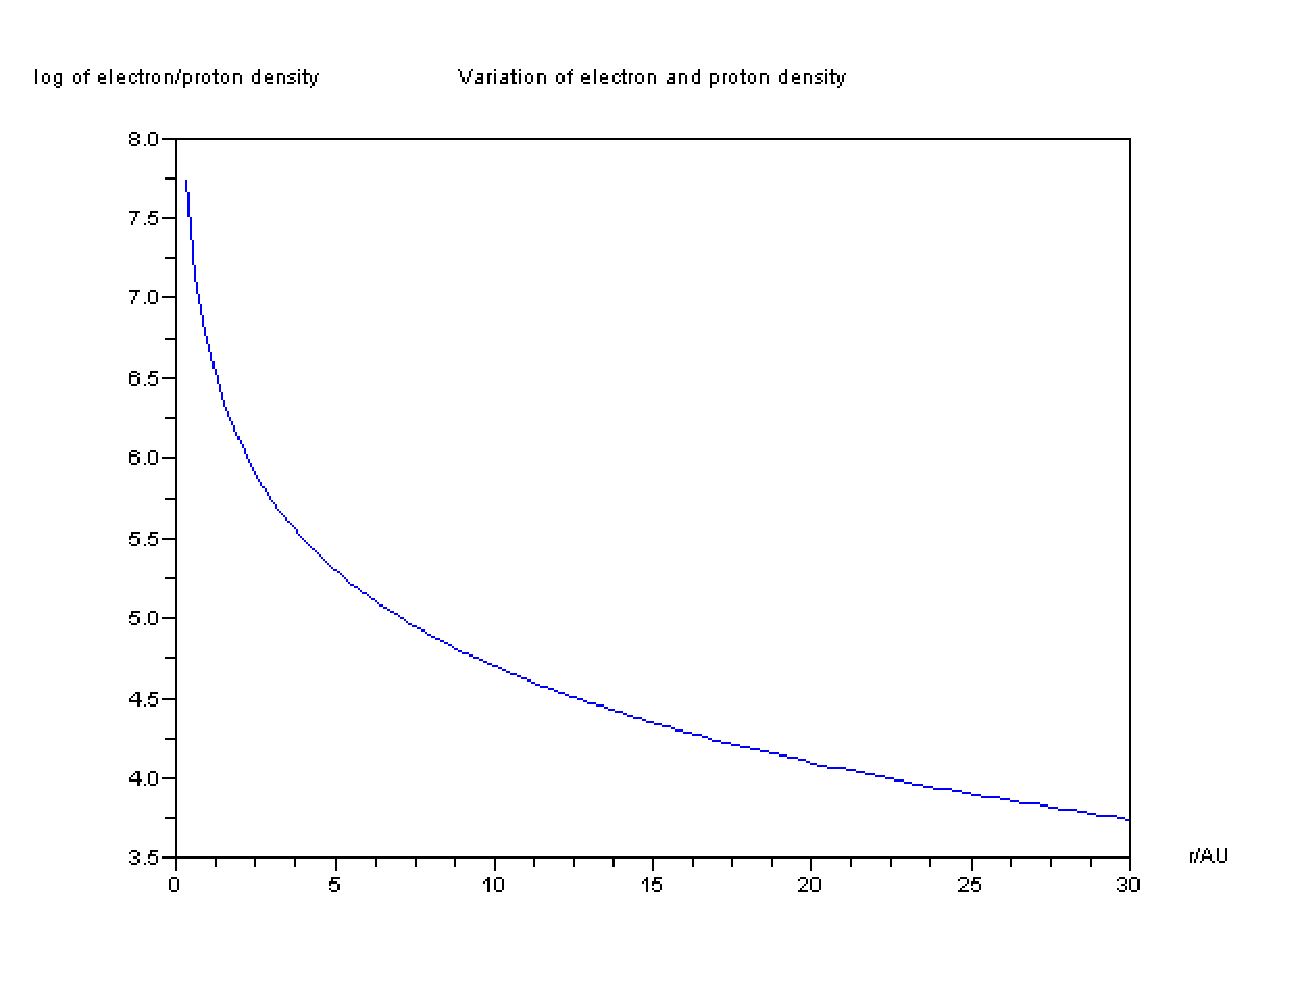
\includegraphics[width=12cm]{pics/electron_number_density_l.eps}\\
  \caption{Logarithmic plot of Electron or proton number density}\label{fig_electron_number_density}
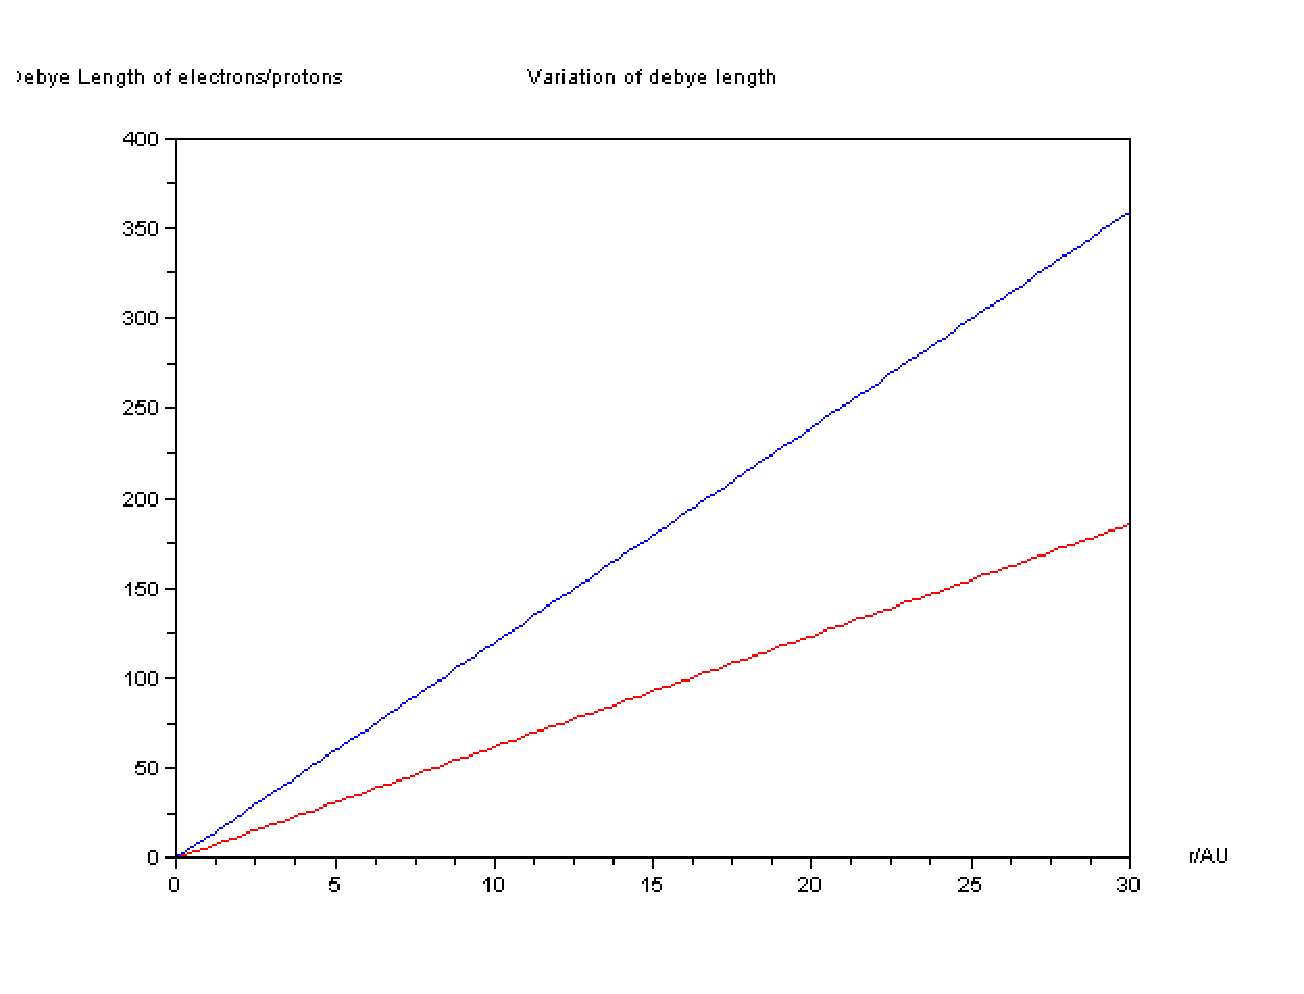
\includegraphics[width=12cm]{pics/debye_length.eps}\\
  \caption{Debye length of electrons (blue) and protons (red)}\label{fig_debye length}
\end{figure}


\begin{figure}
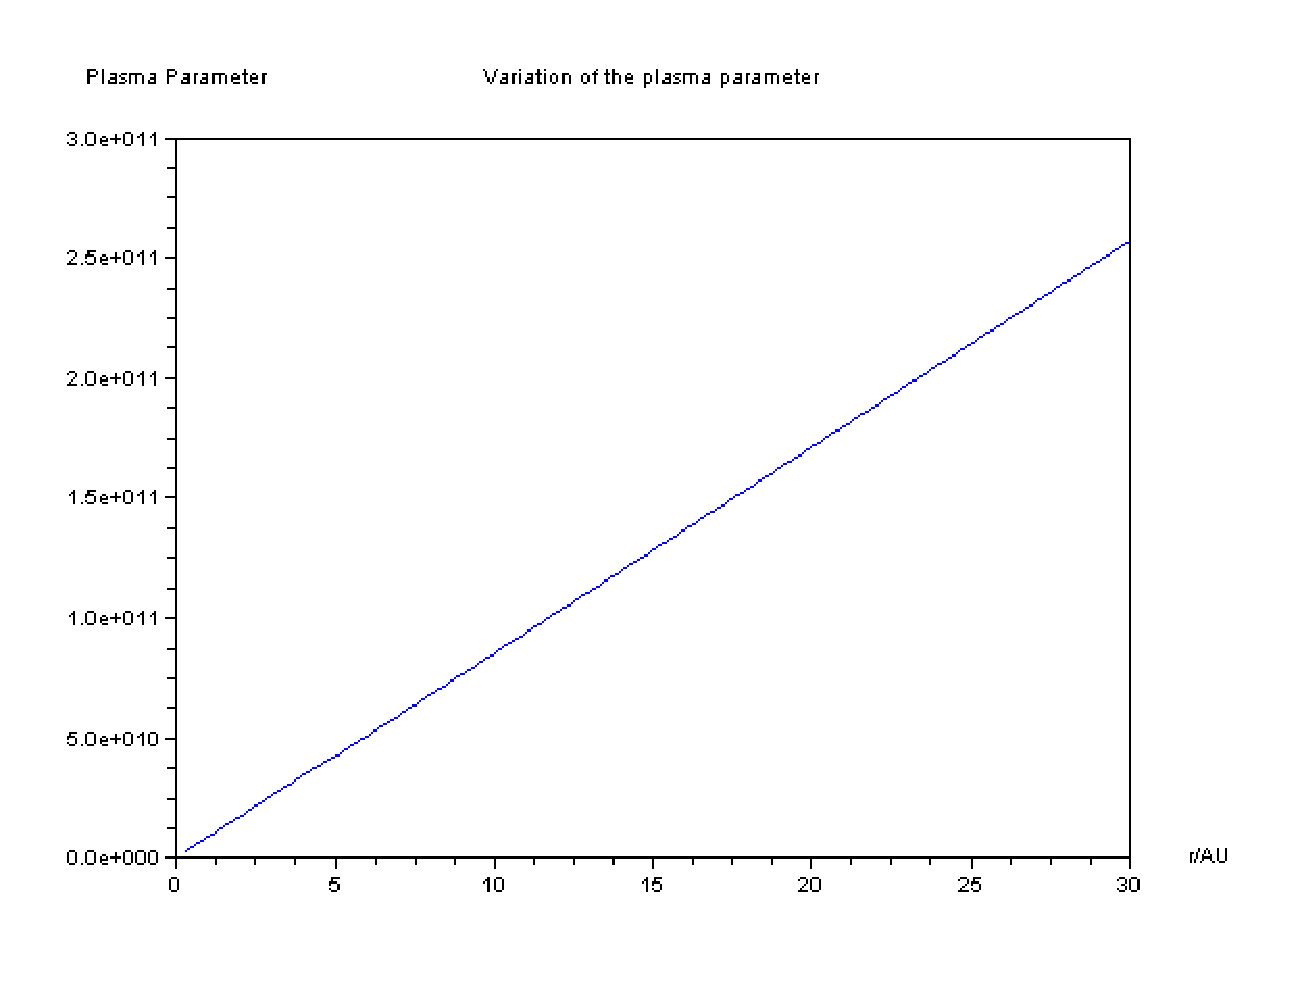
\includegraphics[width=12cm]{pics/plasma_parameter.eps}\\
  \caption{Plasma parameter}\label{fig_plasma_parameter}
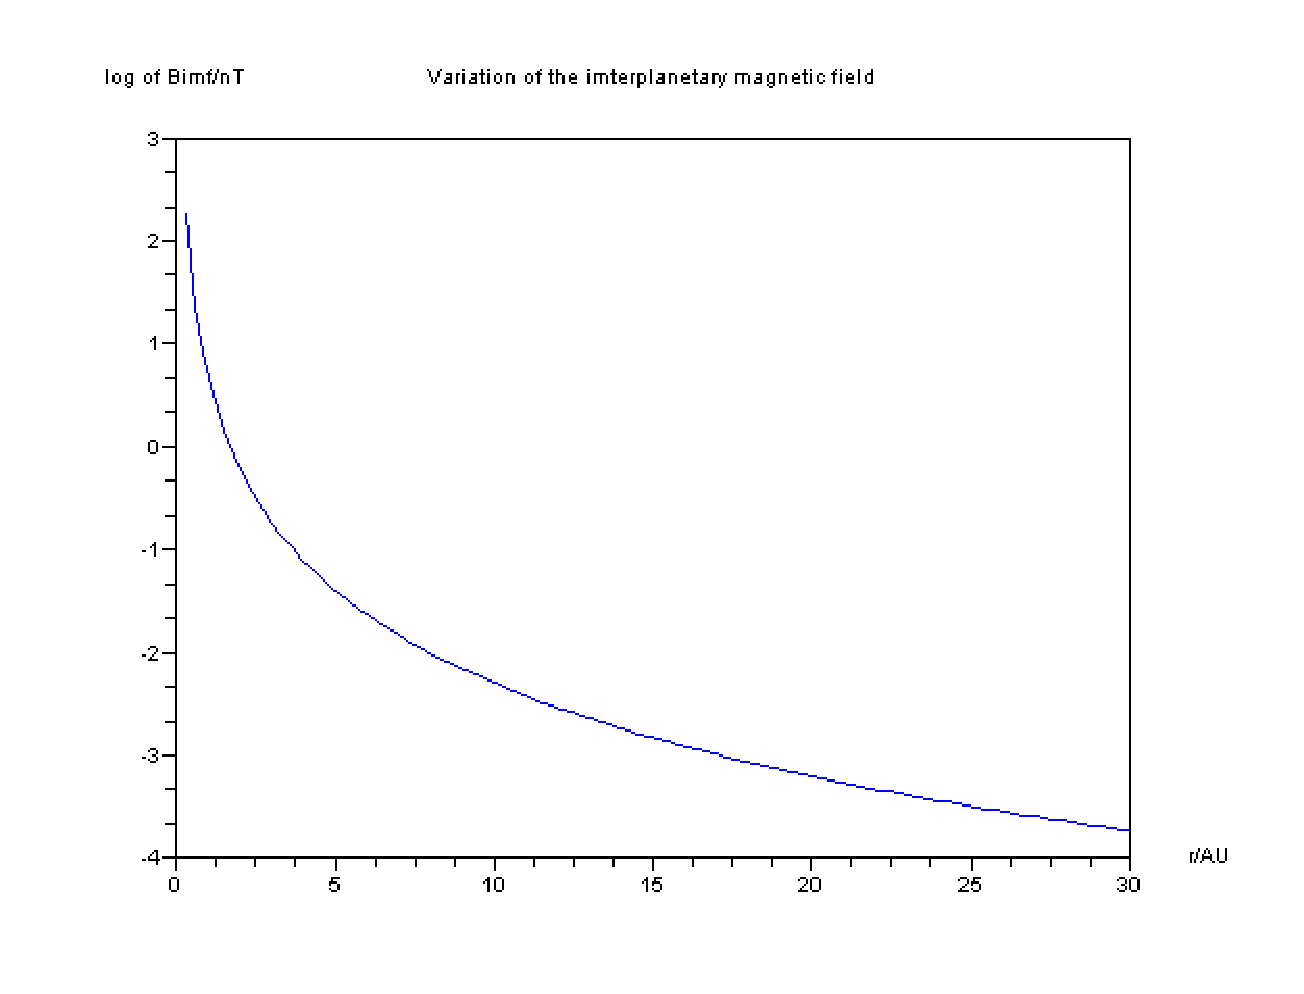
\includegraphics[width=12cm]{pics/Bimf_l.eps}\\
  \caption{Logarithmic plot of Interplanetary magnetic field }\label{fig_Bimf}
\end{figure}

A typical value for the interplanetary magnetic field (IMF) is 4-5nT at 1AU. The equation for the magnitude of the magnetic induction of Sun in nano tesla, as a function of distance in AUs, on the solar equatorial plane is

\begin{equation}\label{Bimf}
    B=\frac{5}{r^3}
\end{equation}

Figure \ref{fig_Bimf} shows its variation with distance from the sun.\\




\begin{figure}
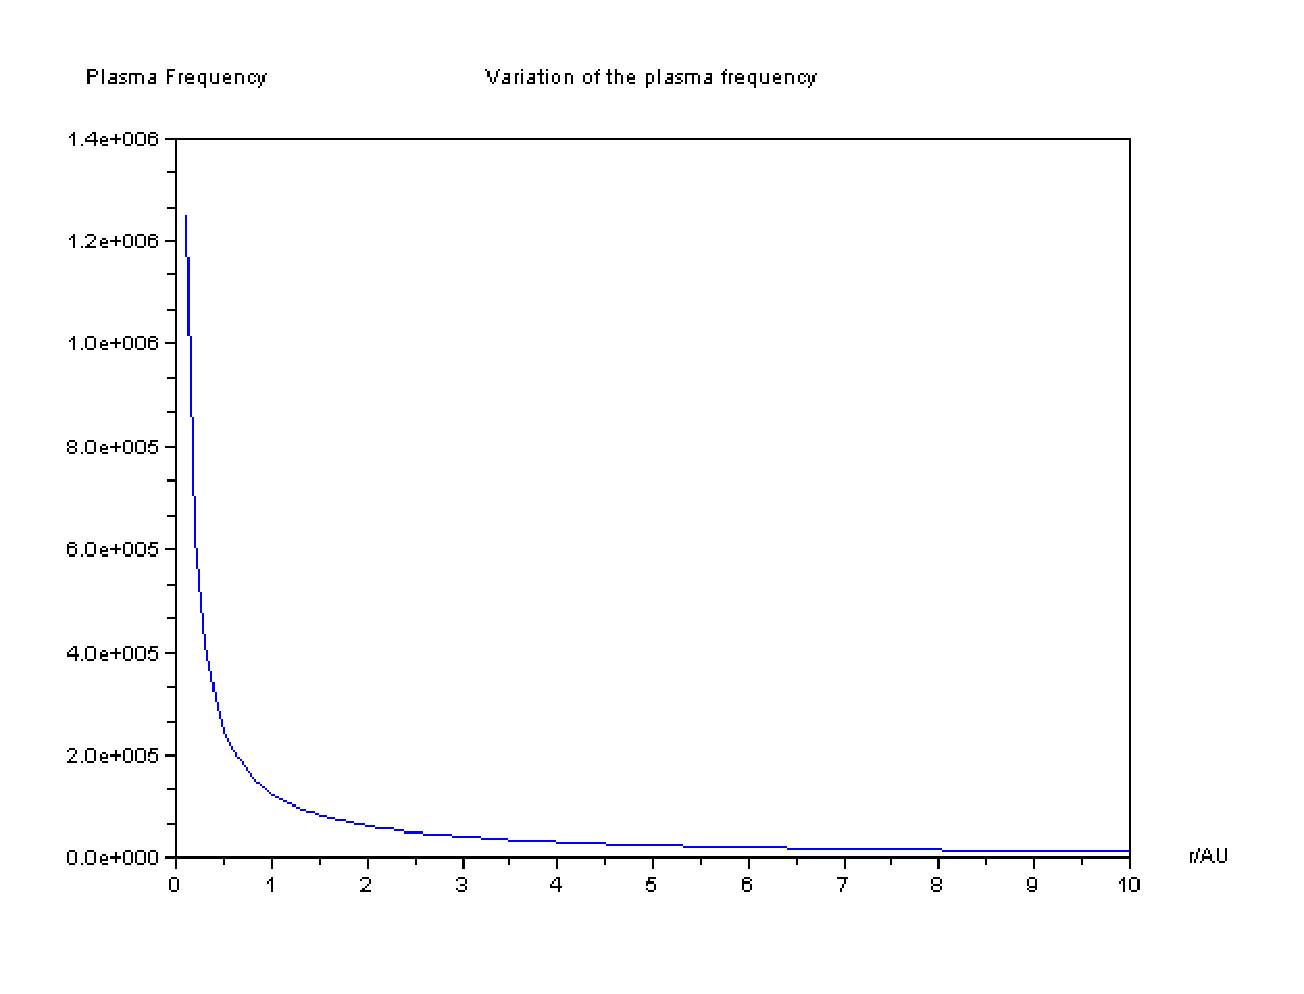
\includegraphics[width=12cm]{pics/plasma_frequency_1.eps}\\
  \caption{Plasma Frequency}\label{fig_plasma_frequency1}
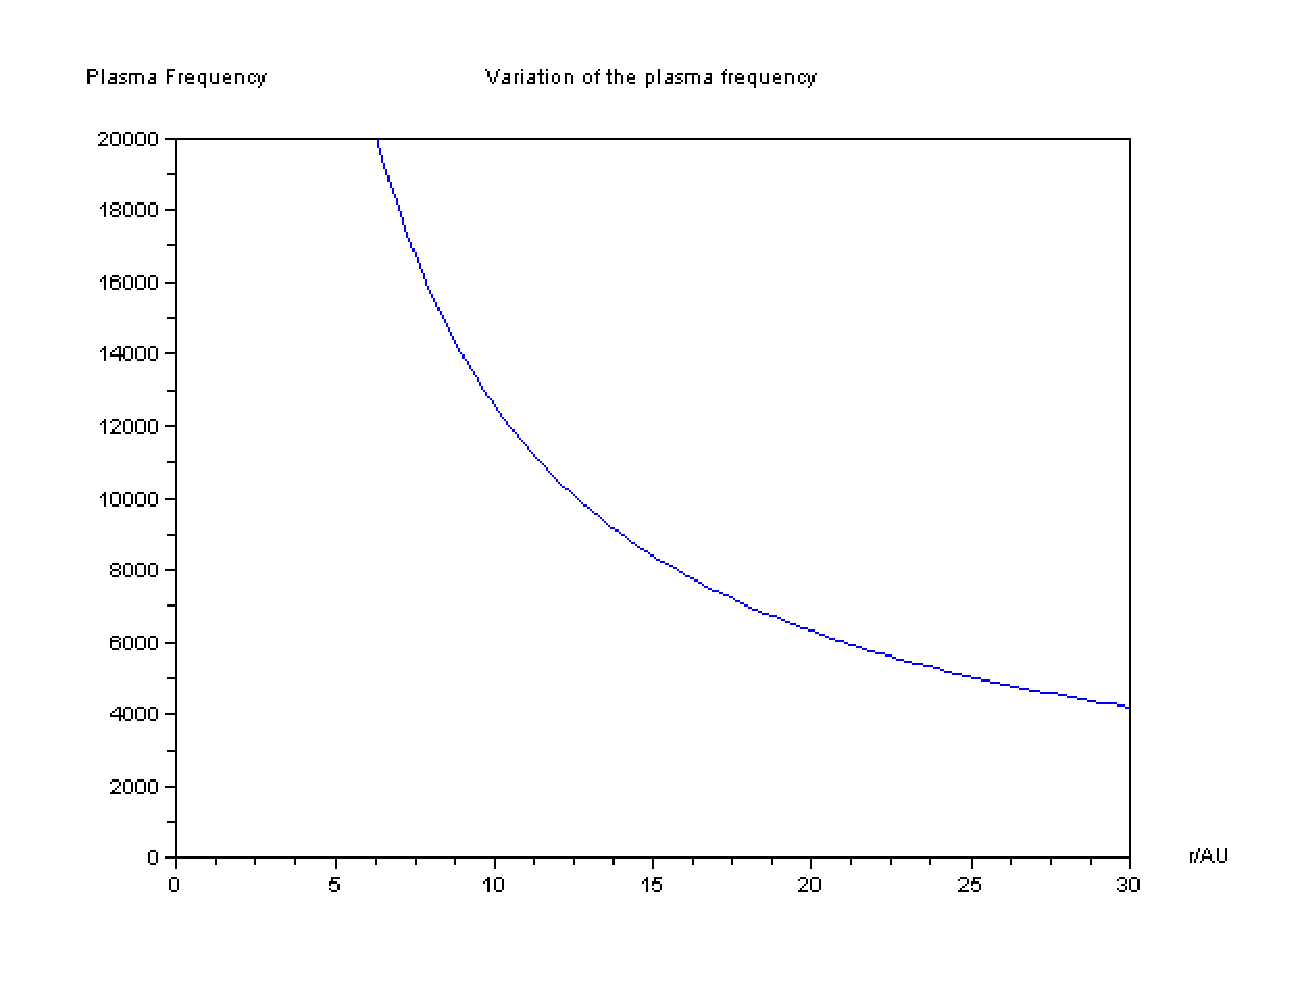
\includegraphics[width=12cm]{pics/plasma_frequency_2.eps}\\
  \caption{Plasma Frequency}\label{fig_plasma_frequency2}
\end{figure}


\begin{figure}
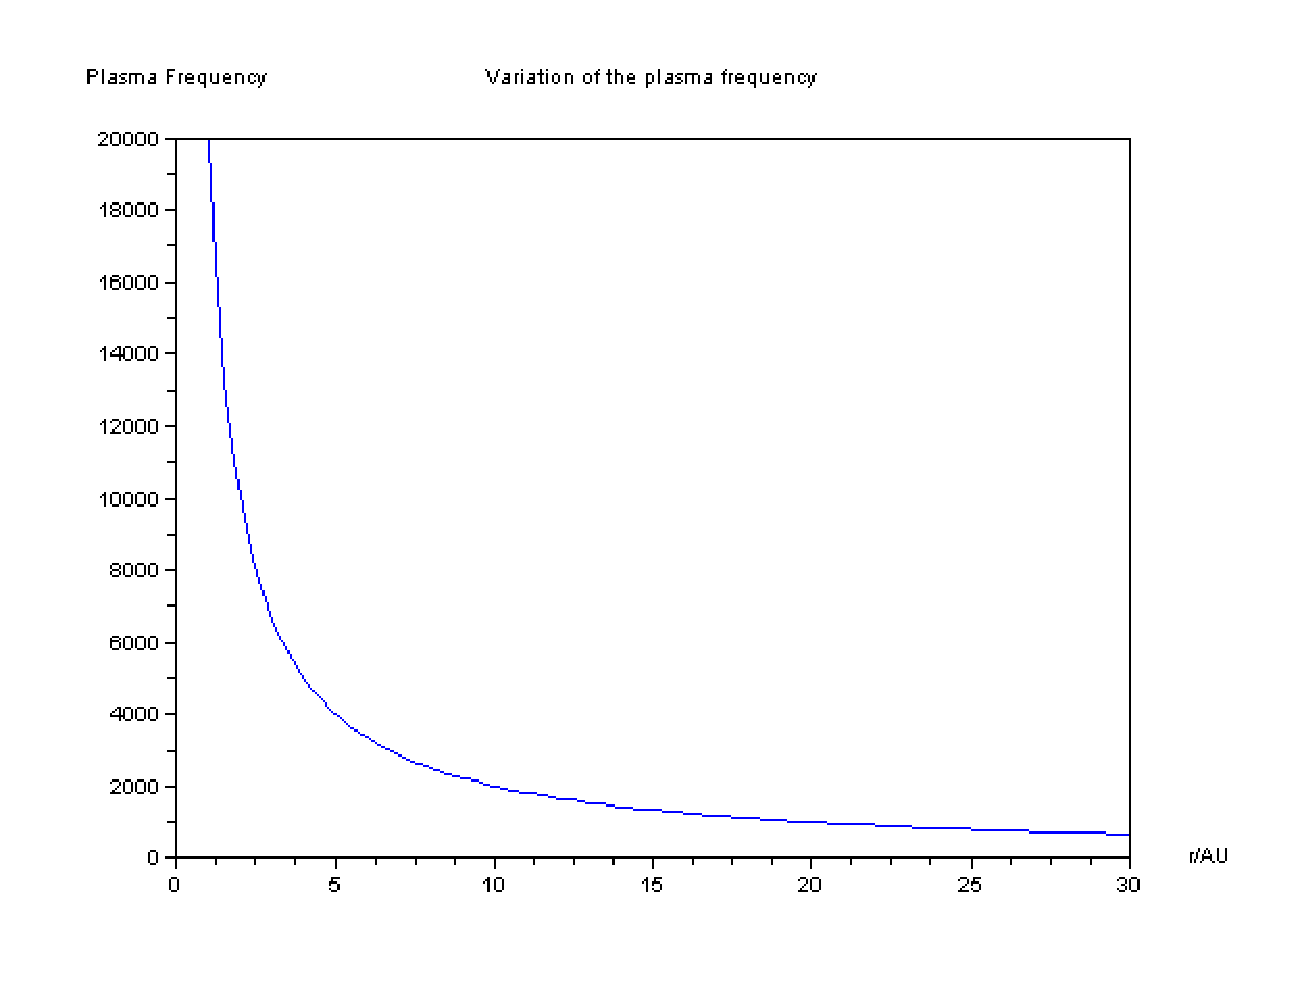
\includegraphics[width=12cm]{pics/plasma_frequency_3.eps}\\
  \caption{Plasma Frequency }\label{fig_plasma_frequency3}
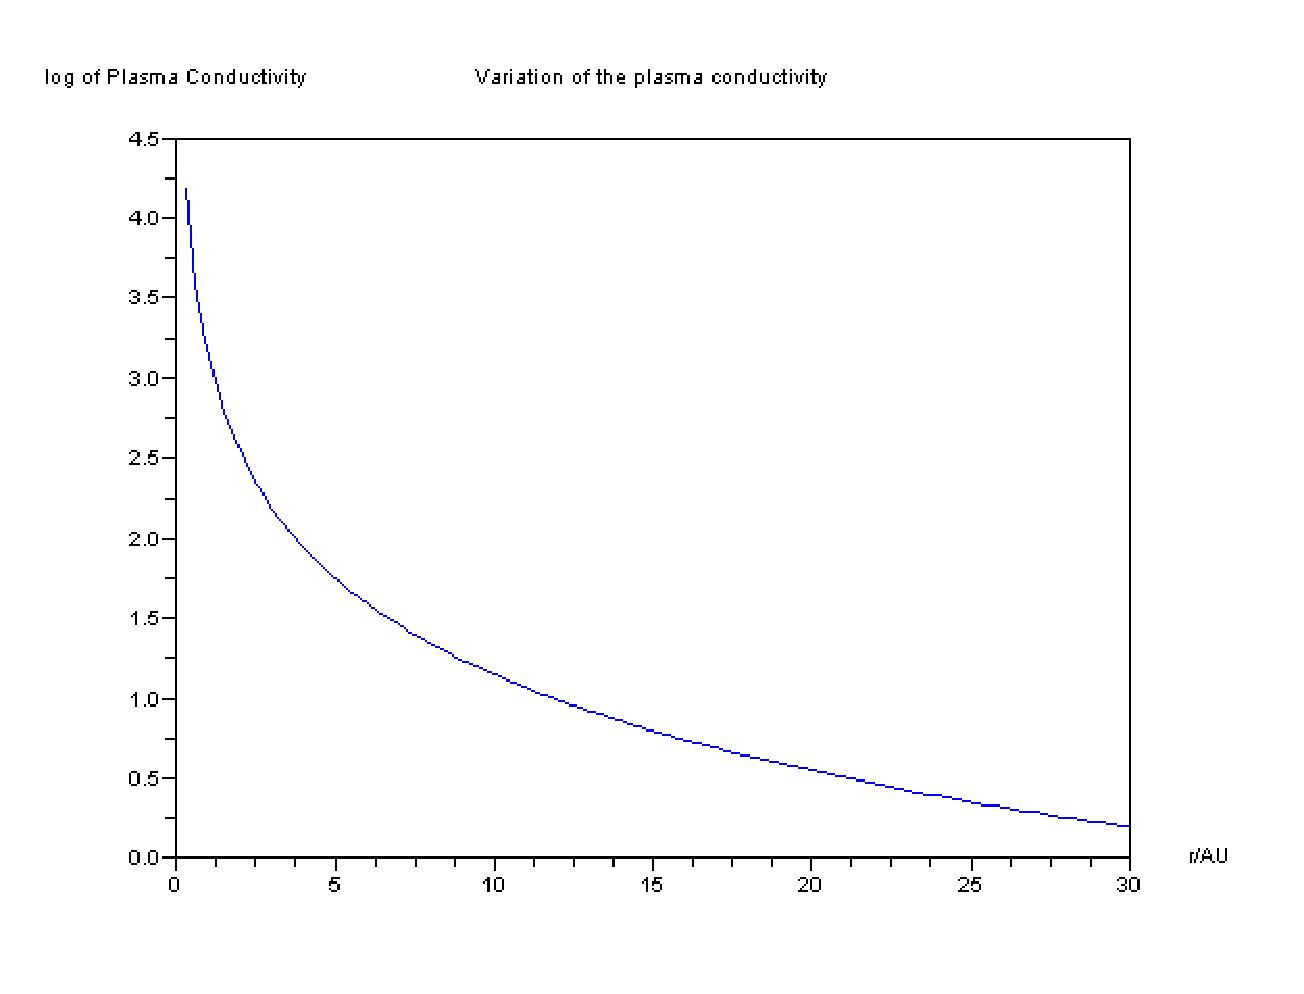
\includegraphics[width=12cm]{pics/conduct_l.eps}\\
\caption{Logarithmic plot of the Plasma Conductivity}\label{fig_plasma_conductivity}
\end{figure}




Figures \ref{fig_plasma_frequency1} and \ref{fig_plasma_frequency2} show $\omega_p$, while \ref{fig_plasma_frequency3} shows $f_p$.\\

A typical value for the collision frequency in the solar wind is $10^{-5}Hz$. When using equation \ref{plasma_conductivity}, the range of the conductivity is shown in figure \ref{fig_plasma_conductivity}.\\

The plasma beta is the relation of kinetic to magnetic pressure (\ref{fig_plasma_beta}).

\begin{equation}\label{plasma_beta}
    \beta=\frac{nkT}{\frac{B^2}{2\mu_0}}
\end{equation}

\begin{figure}
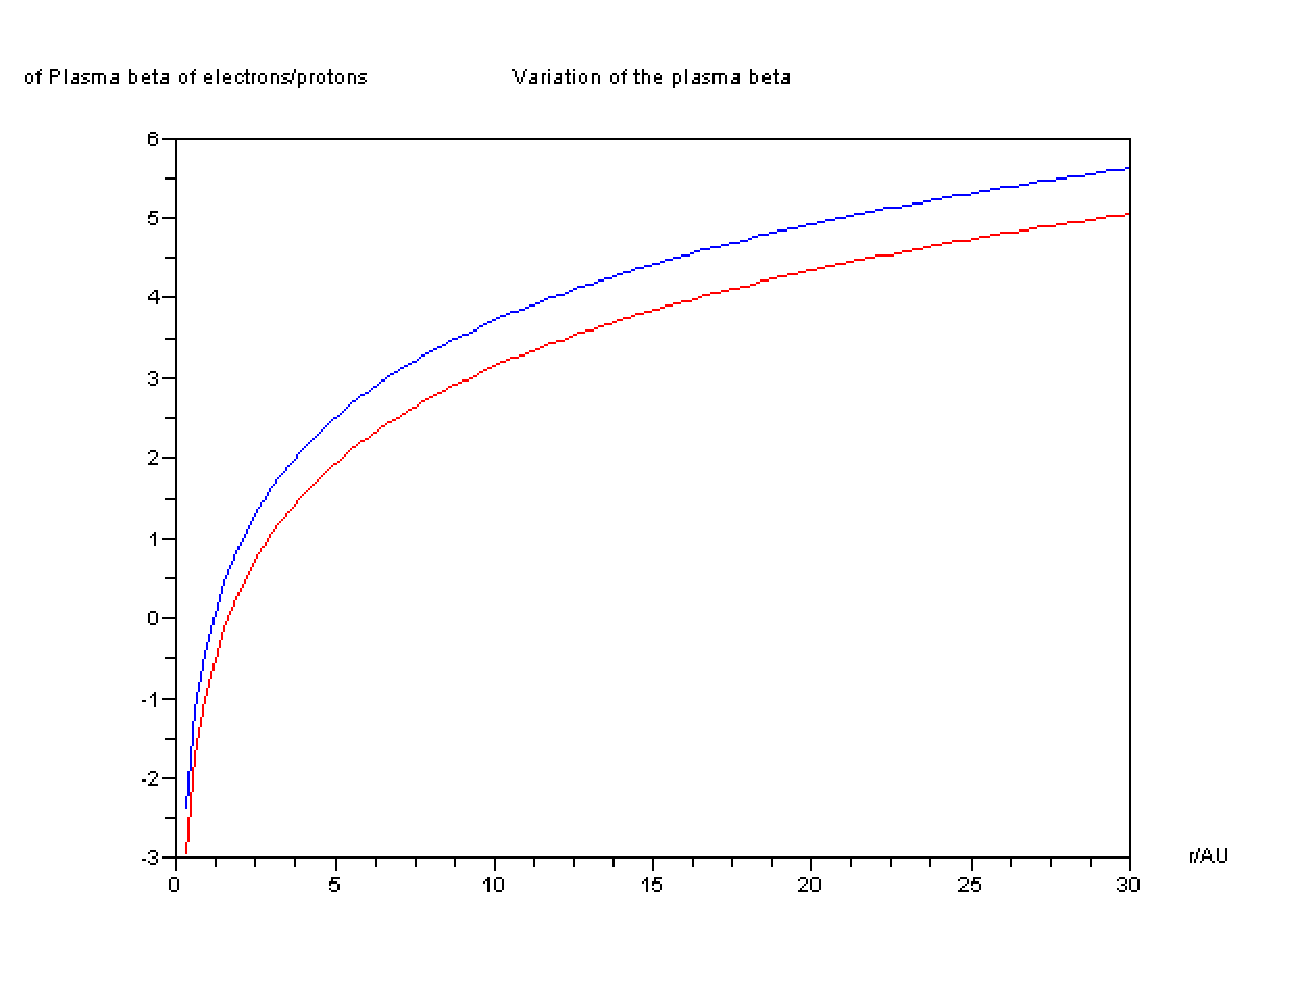
\includegraphics[width=12cm]{pics/plasma_beta_l.eps}\\
  \caption{Logarithmic plot of the Plasma Beta}\label{fig_plasma_beta}
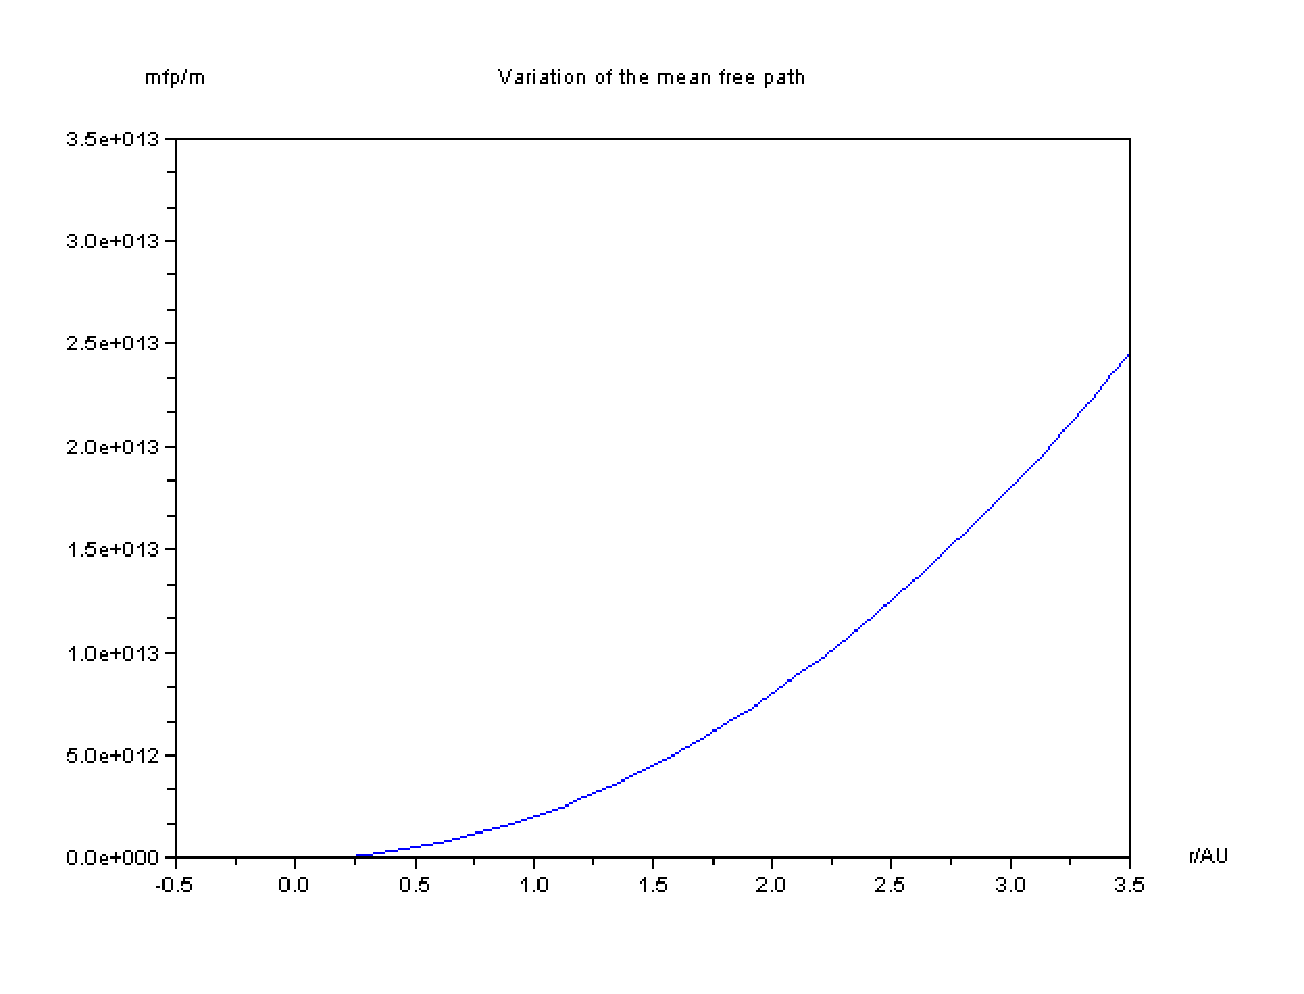
\includegraphics[width=12cm]{pics/mfp1.eps}\\
  \caption{Mean free path}\label{fig_mfp_anfang}
\end{figure}



The speed of sound can be computed as

\begin{equation}\label{v_s}
    v_s=\sqrt{\gamma \frac{p}{\rho}}=\sqrt{\gamma \frac{nk(T_e+T_p)}{nm}}=\sqrt{\gamma \frac{k(T_e+T_p)}{m}}\thickapprox 50 kms^{-1}
\end{equation}

where m is the proton mass. Since the number density cancels, the speed of sound is independent from the distance from the Sun.\\

The mean free path is

\begin{equation}\label{mfp}
    \lambda_f=\frac{1}{n \sigma_{eff}}
\end{equation}

where $ \sigma_{eff}\approx 10^{-19}m^2$ is the effective cross section of the particles. The result is in figures \ref{fig_mfp_anfang}-\ref{fig_mfp_ende}.



\begin{figure}
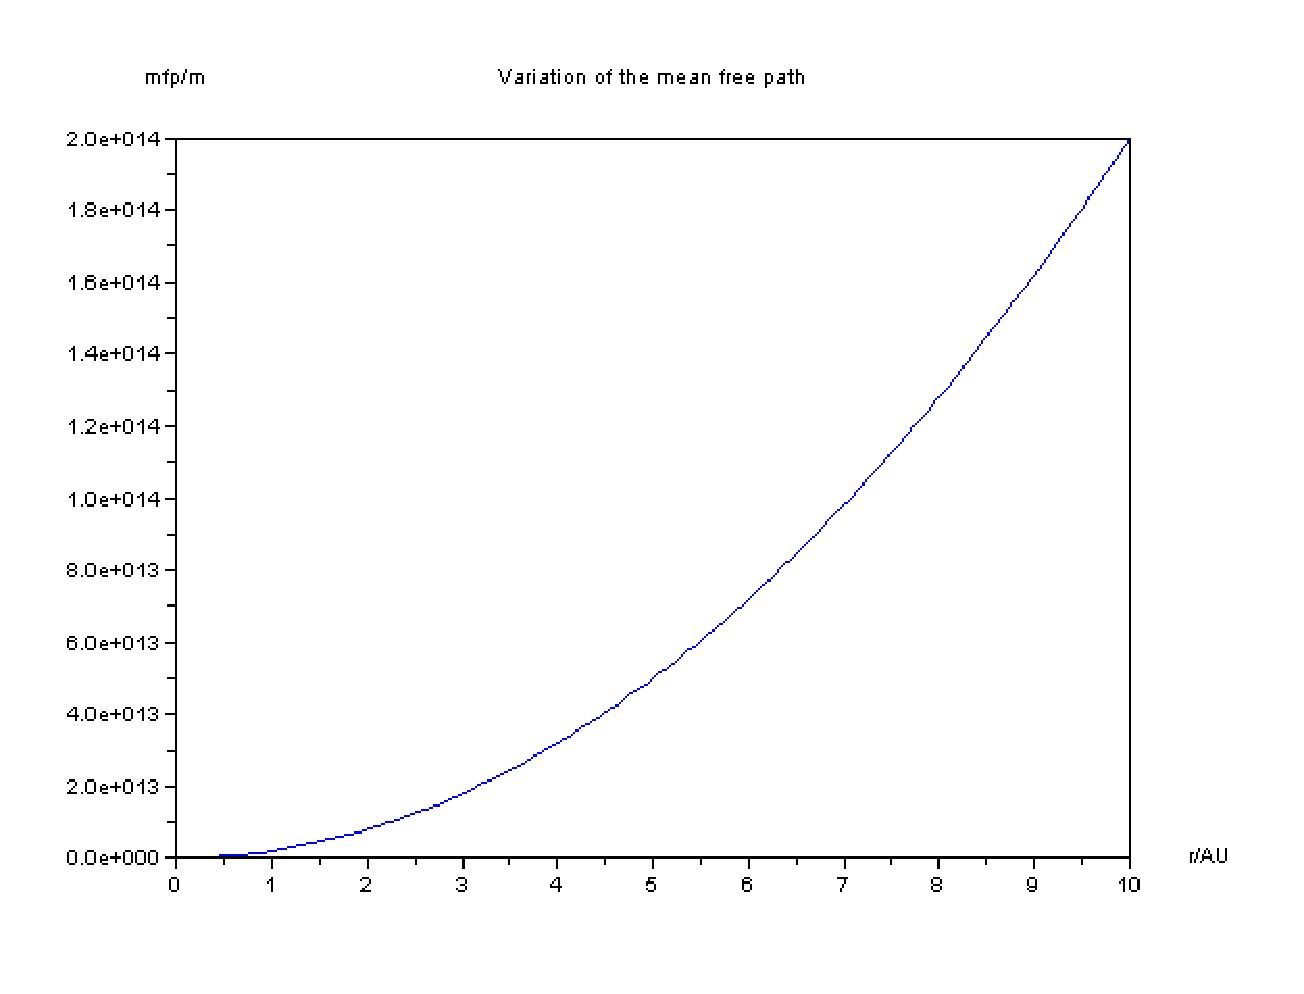
\includegraphics[width=12cm]{pics/mfp2.eps}\\
\caption{Mean free path}
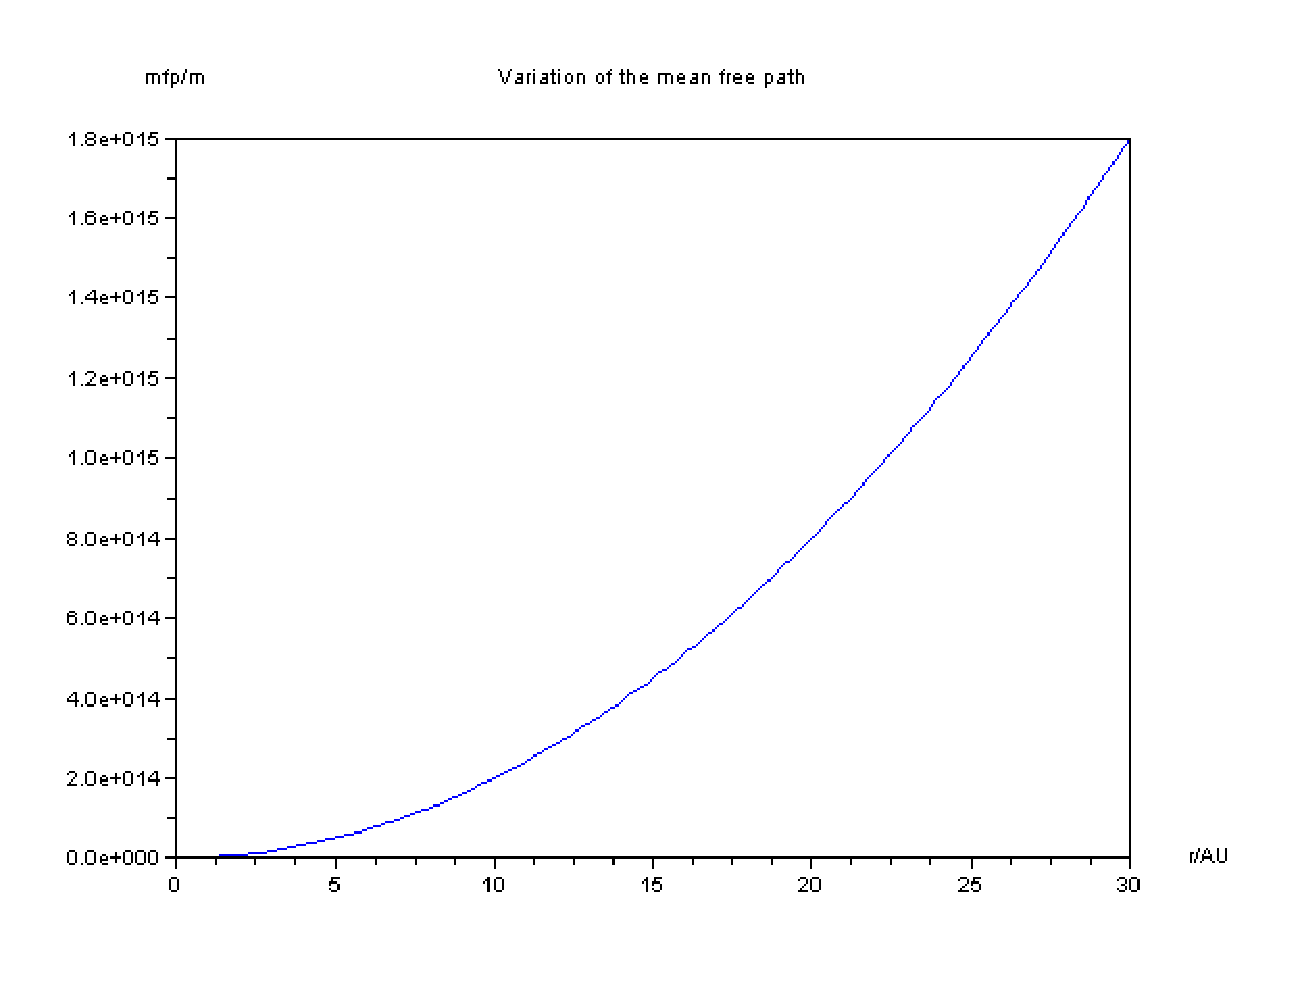
\includegraphics[width=12cm]{pics/mfp3.eps}\\
\caption{Mean free path}\label{fig_mfp_ende}
\end{figure}

The cyclotron radius has a dimension of

\begin{equation}\label{r_c}
    r_c=\frac{mv}{eB}sin{\alpha}
\end{equation}

where $\alpha$ is the pitch angle. The cyclotron frequency is

\begin{equation}\label{omega_c}
    \omega_c=\frac{eB}{m}
\end{equation}

See figures \ref{fig_omegac} and \ref{fig_omegac_p}.\\

\begin{figure}
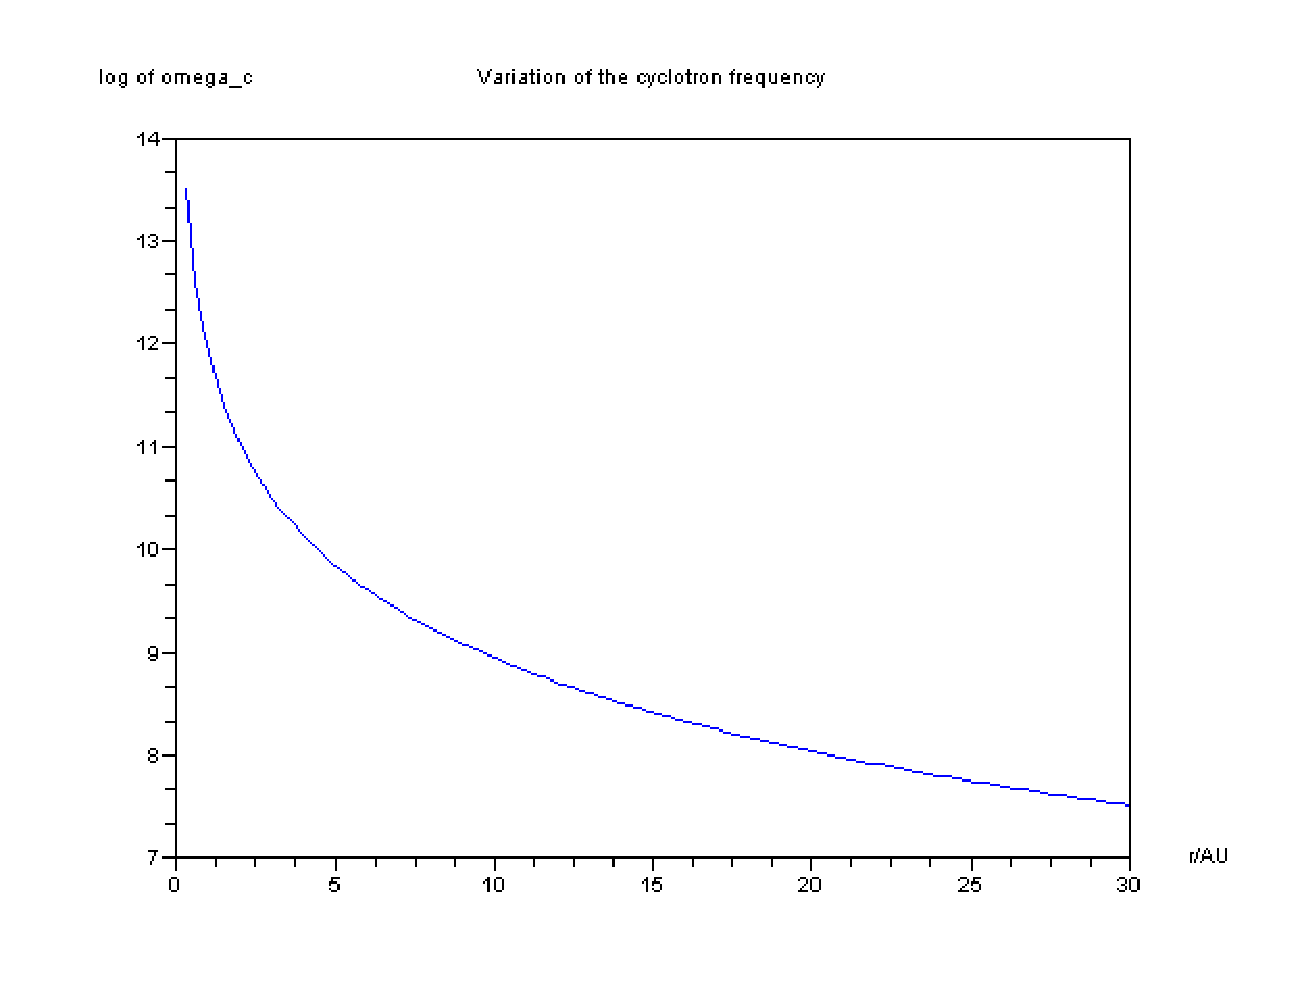
\includegraphics[width=12cm]{pics/omega_c_l.eps}\\
\caption{Logarithmic plot of the Cyclotron frequency for electrons}\label{fig_omegac}
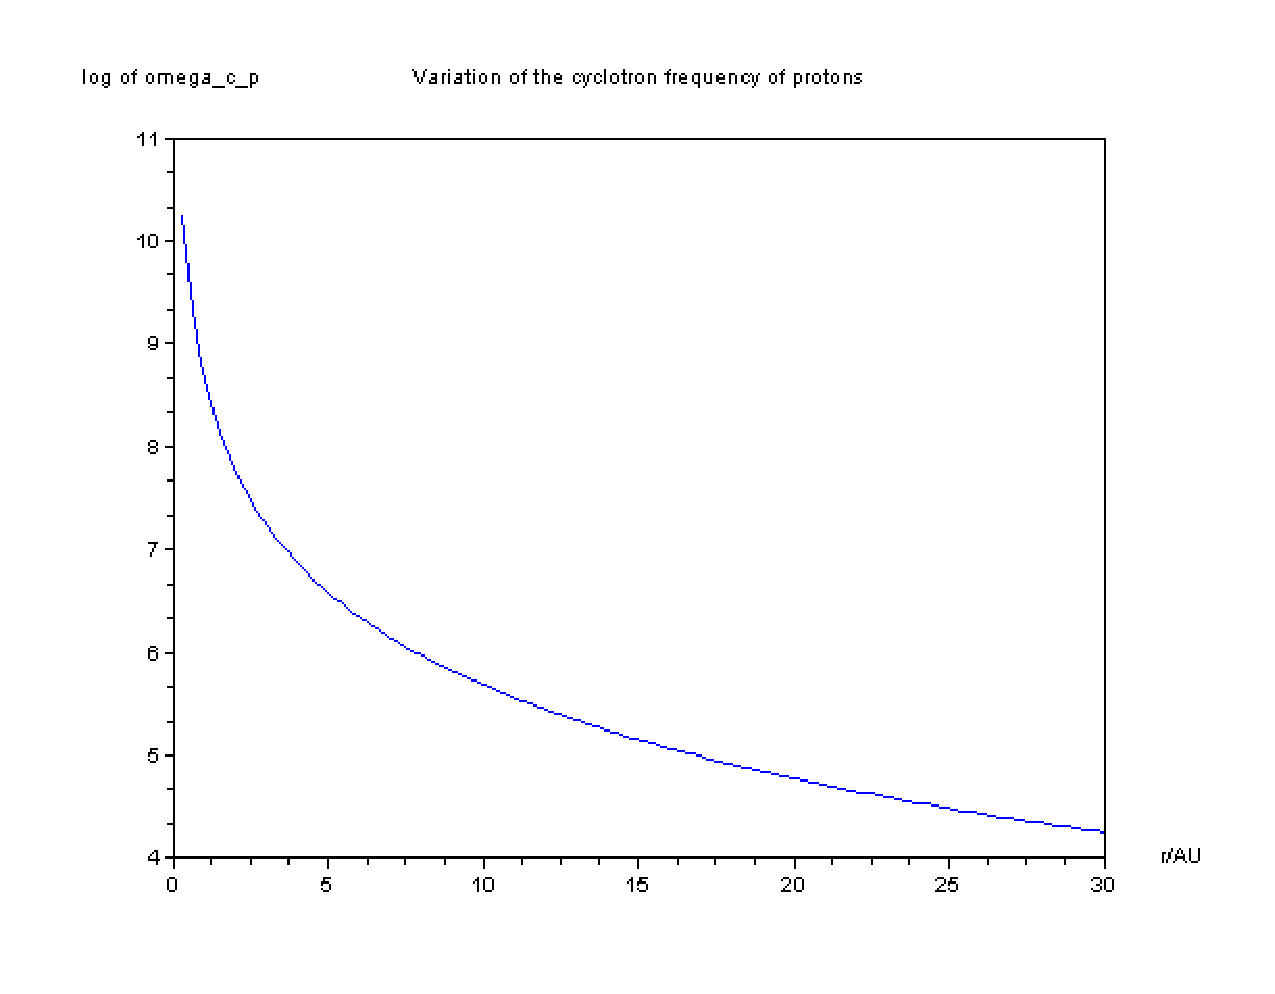
\includegraphics[width=12cm]{pics/omega_c_l_p.eps}\\
\caption{Logarithmic plot of the Cyclotron frequency for protons}\label{fig_omegac_p}
\end{figure}


\chapter{Modeling the antenna}
The antennas used in space vehicles such as stereo or bepi colombo can be modeled as simple antenna elements (monopoles, dipoles, loops, spheres) in an infinite medium. In the second instance the model can be refined using a wiregrid that comprises many basic elements.


\chapter{Thermal noise spectroscopy}
\cite{meiervernet1}\\

Thermal noise spectroscopy is a technique for finding the basic parameters of plasma by analyzing the electrostatic field spectrum measured by antennas. When the plasma frequency is higher than the cyclotron frequency, thermal motion  excites Langmuir waves that are dependent of the velocity distribution function. The dispertion relations can be seen at (\ref{langmuir_disp_rel1}) and (\ref{langmuir_dispersion_relation2}). The spectrum is cut off at $\omega_p$ and has a peak just above. The cutoff bears information about the plasma density, the spectrum level about the temperature. The form of the peak reveals information about the supra thermal electrons. Figure \ref{fig_thermal_noise} shows an example and also one of the problems with thermal noise. Its intensity is normally higher than the intensity of many received radio emissions (a type 2 burst in this example).\\



\begin{figure}
  % Requires \usepackage{graphicx}
  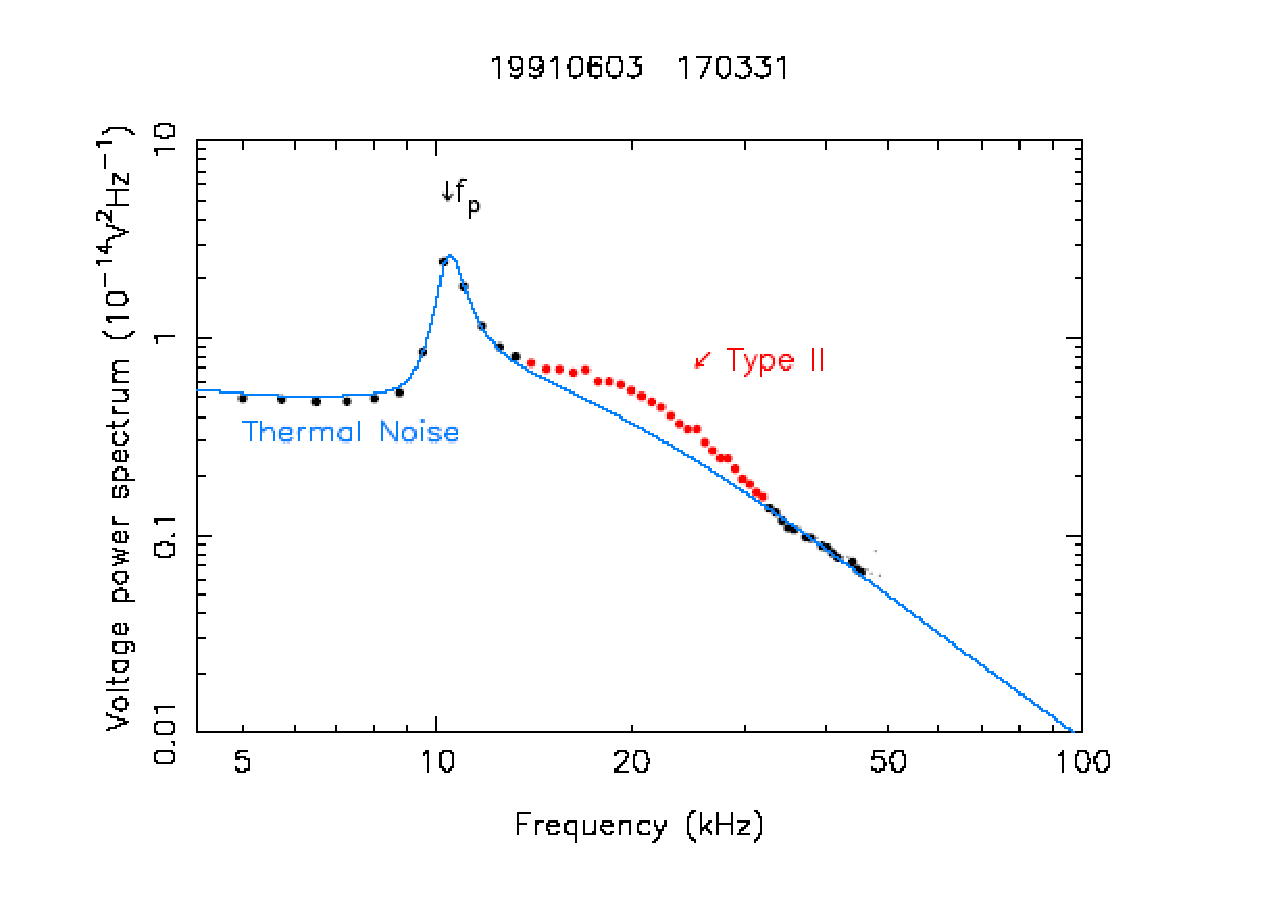
\includegraphics[width=12cm]{pics/thermal-noise.eps}\\
  \caption{Thermal noise spectrum}\label{fig_thermal_noise}
\end{figure}


\part{Single particle effects}
\chapter{Effect of a single charge in the rest frame of a metal surface}
\section{A charge near a conducting, grounded sphere}
\subsection{The charge distribution}

The method of imaging charge is used to compute the surface charge distribution (source: \cite{jackson}). (fig. \ref{fig_chargenearsphere}). Determine potential such that it is zero at r=a.

\begin{eqnarray}\label{potential_chargenearsphere}
    \Phi(\mathbf{r})&=&\frac{q}{|\mathbf{r}-\mathbf{x}|}+\frac{q'}{|\mathbf{r}-\mathbf{x'}|}
    \\
    &=&\frac{q}{|r\mathbf{\hat{r}}-x\mathbf{\hat{x}}|}+\frac{q'}{|r\mathbf{\hat{r}}-x'\mathbf{\hat{x}}|}=0\nonumber
\end{eqnarray}


\begin{figure}
  % Requires \usepackage{graphicx}
  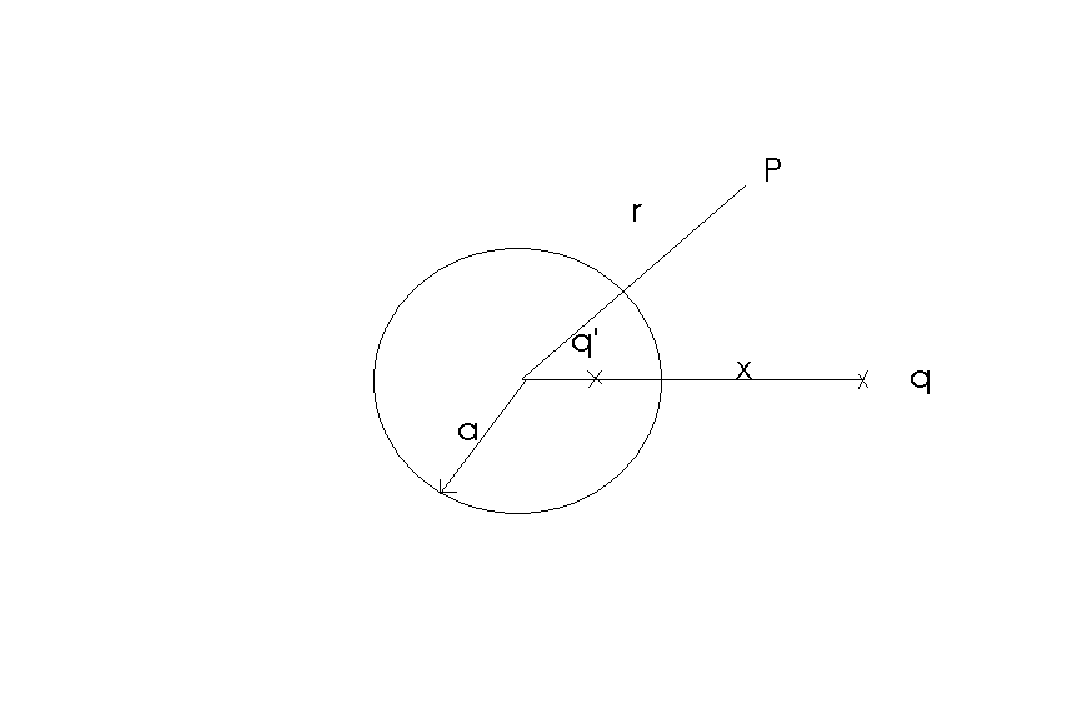
\includegraphics[width=12cm]{pics/chargenearsphere.eps}\\
  \caption{Charge q near sphere}\label{fig_chargenearsphere}
\end{figure}

\paragraph*{}
At $r=a$:
\begin{eqnarray}\label{potential_chargenearsphere_2}
    \Phi(\mathbf{r=a})&=&\frac{q}{|a\mathbf{\hat{r}}-x\mathbf{\hat{x}}|}+\frac{q'}{|a\mathbf{\hat{r}}-x'\mathbf{\hat{x}}|}
    \\
&=&\frac{q}{a|\mathbf{\hat{r}}-\frac{x}{a}\mathbf{\hat{x}}|}+\frac{q'}{x'|\mathbf{\frac{a}{x'}\hat{r}}-\mathbf{\hat{x}}|}\nonumber
\\
&=&\frac{q}{a|\mathbf{\hat{r}}-\frac{x}{a}\mathbf{\hat{x}}|}+\frac{q'}{x'|\mathbf{\hat{x}}-\mathbf{\frac{a}{x'}\hat{r}}|}=0\nonumber
\end{eqnarray}

\paragraph*{}
To vanish on the whole sphere,

\begin{eqnarray}
% \nonumber to remove numbering (before each equation)
  \frac{q}{a} &=& -\frac{q'}{x'} \\
\frac{x}{a} &=& \frac{a}{x'}
\end{eqnarray}


\paragraph*{}
For the position and charge of the image charge, this is

\begin{eqnarray}
% \nonumber to remove numbering (before each equation)
  q' &=& - a \frac{q}{x} \\
x' &=& \frac{a^2}{x}
\end{eqnarray}

\paragraph*{}
So when a charge approaches at infinity, the image starts with a vanishing small magnitude at the center of the sphere. As the charge comes closer, the image proceeds to the boundary of the sphere and increases in magnitude. The two charges meet at the boundary where they have equal magnitude.

\paragraph*{}
Due to symmetry reasons, all this can be translated to the case of a cylindrical shape (antenna), when the particle approaches from the equatorial plane (EP). If it approaches from the side of the EP, the tip has to be used as surface form (half sphere ?). At the tip of the antenna, the process is similar, where the radius of the sphere has to be substituted for by the curvature radius. When the particle is below the EP, the image has to be calculated for the spacecraft body, which I approximate as a conducting sphere.

\paragraph*{}
The induced surface charge density can be calculated by taking the directional derivative at the surface along the surface normal at the surface. In our case

\begin{eqnarray}
\sigma(\gamma)&=&-\frac{1}{4\pi}\mathbf{\hat{r}}\cdot \nabla \Phi(\mathbf{r}=a) \label{surface charge _chargenearsphere} \\
&=& -\frac{1}{4\pi}\mathbf{\hat{r}}\cdot \nabla \left[ \frac{q}{|\mathbf{r}-\mathbf{x}|} +\frac{q'}{|\mathbf{r}-\mathbf{x'}|} \right] \nonumber
\\
&=& -\frac{1}{4\pi}\mathbf{\hat{r}}\cdot \nabla \left[ \frac{q}{|\mathbf{r}-\mathbf{x}|}-\frac{ \frac{a}{x} q}
{|\mathbf{r}- \frac{a^2}{x}\mathbf{\hat{x}}|} \right] \nonumber
\\
&=& -\frac{q}{4\pi}\mathbf{\hat{r}}\cdot \nabla \left[ \frac{1}{|\mathbf{r}-\mathbf{x}|}-\frac{ \frac{a}{x} }
{|\mathbf{r}- \frac{a^2}{x}\mathbf{\hat{x}}|} \right] \nonumber
\\
&=& -\frac{q}{4\pi}\mathbf{\hat{r}}\cdot \left[ \frac{-(\mathbf{r}-\mathbf{x})}{|\mathbf{r}-\mathbf{x}|^3}-\frac{ -\frac{a}{x} (\mathbf{r}- \frac{a^2}{x}\mathbf{\hat{x}})}
{|\mathbf{r}- \frac{a^2}{x}\mathbf{\hat{x}}|^3} \right] \nonumber
\\
&=& \frac{q}{4\pi}\mathbf{\hat{r}}\cdot \left[ \frac{(\mathbf{r}-\mathbf{x})}{(r^2+x^2-2rx\cos \gamma)^\frac{3}{2}}-\frac{ \frac{a}{x} (\mathbf{r}- \frac{a^2}{x}\mathbf{\hat{x}})}
{(r^2+ \frac{a^4}{x^2} -2 \frac{ra^2}{x}\cos \gamma)^\frac{3}{2}} \right] \nonumber
\\
&=& \frac{q}{4\pi} \left[ \frac{(r-x\cos \gamma)}{(r^2+x^2-2rx\cos \gamma)^\frac{3}{2}}-\frac{ \frac{a}{x} (r- \frac{a^2}{x}\cos \gamma)}
{(r^2+ \frac{a^4}{x^2} -2 \frac{ra^2}{x}\cos \gamma)^\frac{3}{2}} \right] \nonumber
\end{eqnarray}

\paragraph*{}
At $r=a$:

\begin{eqnarray}
\sigma(\gamma)_{r=a}&=& \frac{q}{4\pi a^2} \left[ \frac{(1-\frac{x}{a}\cos \gamma)}{(1+\frac{x^2}{a^2}-2\frac{x}{a}\cos \gamma)^\frac{3}{2}}-\frac{ \frac{a}{x} (1- \frac{a}{x}\cos \gamma)}{(1+ \frac{a^2}{x^2} -2 \frac{a}{x}\cos \gamma)^\frac{3}{2}} \right]
\end{eqnarray}


\begin{figure}
  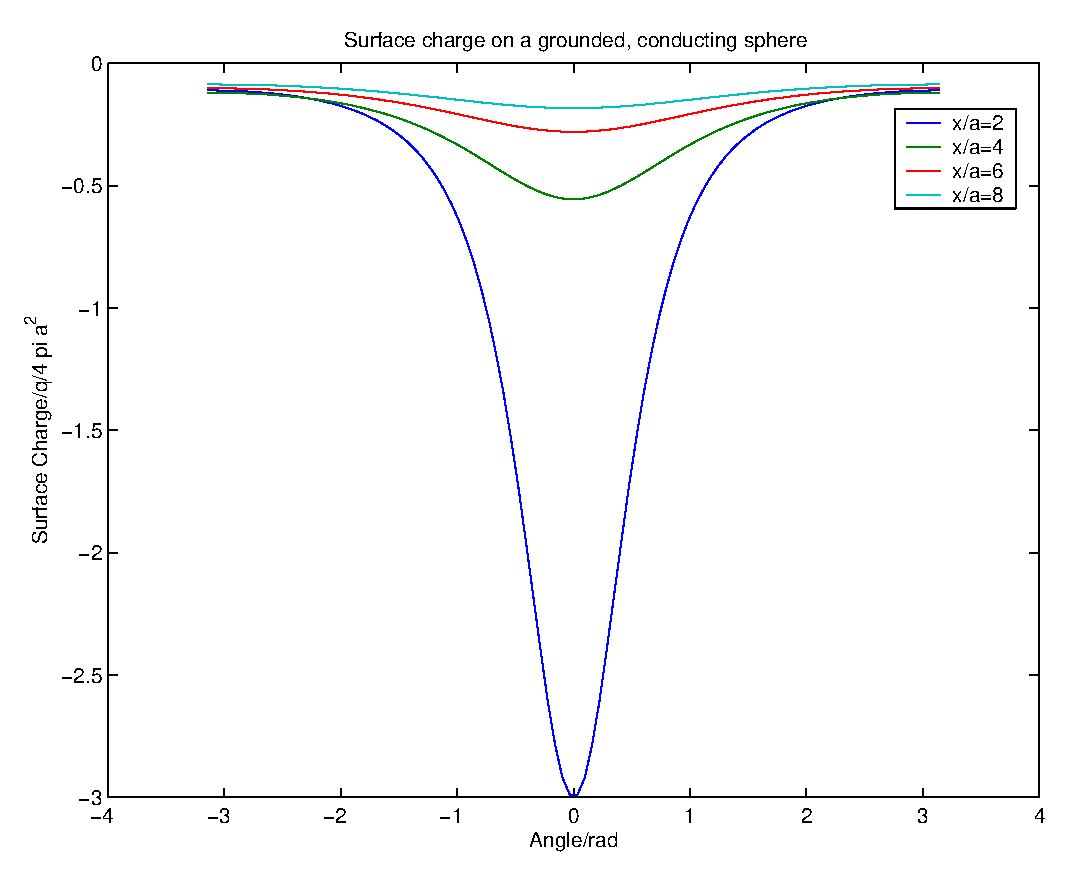
\includegraphics[width=12cm]{pics/surf_charge_conduct_ground_sphere.eps}\\
  \caption{Surface charge, induced on a grounded conducting sphere by a single charge}\label{fig_surf_charge_conduct_ground_sphere}
\end{figure}

\paragraph*{}
The integral around the sphere is q.

\subsection{The force}
\paragraph*{}
The force between the charge and the sphere is calculated with Coulomb's law between the charge and the image charge.

\begin{eqnarray}
F(q,q',\mathbf{x})&=& \frac{1}{4 \pi \varepsilon_0} \frac{qq' (\mathbf{x}-\mathbf{x'})}{|\mathbf{x}-\mathbf{x'}|^3}
\\
&=& -\frac{1}{4 \pi \varepsilon_0} \frac{q^2  \frac{a}{x} (\mathbf{\hat{x}})}{(x-x')^2}\nonumber
\\
&=& -\mathbf{\hat{x}}\frac{1}{4 \pi \varepsilon_0} \frac{a}{x} \frac{q^2   }{(x-\frac{a^2}{x})^2}\nonumber
\\
&=& -\mathbf{\hat{x}}\frac{1}{4 \pi \varepsilon_0} \frac{a q^2 }{x^3(1-\frac{a^2}{x^2})^2} \nonumber
\end{eqnarray}

\paragraph*{}
So the there is an inverse cube law far from the sphere (Fig.\ref{fig_force_on_charge_conduct_ground_sphere}). Near the sruface of the sphere, the force law is an inverse square law, between the surface and the point charge, as shown in the figure. The force is always in a direction to the sphere.

\begin{figure}
  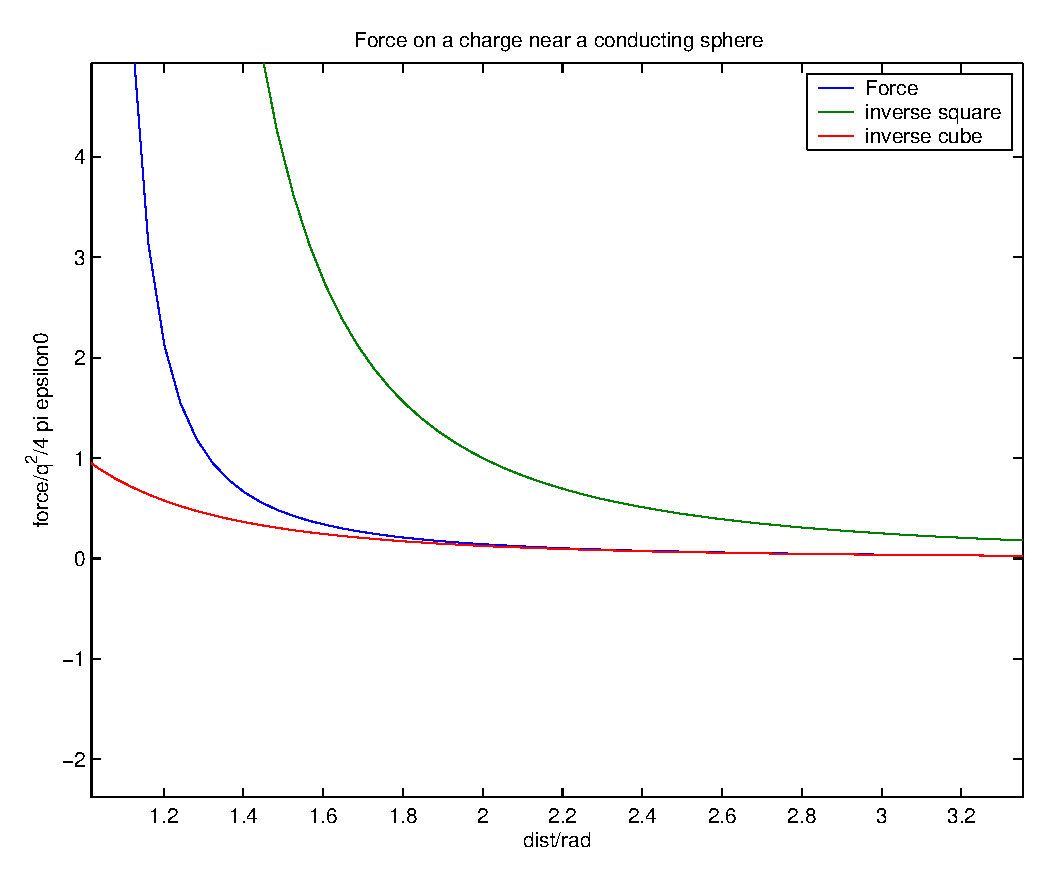
\includegraphics[width=12cm]{pics/force_on_charge_conduct_ground_sphere.eps}\\
  \caption{Force on a charge near a grounded conducting sphere}\label{fig_force_on_charge_conduct_ground_sphere}
\end{figure}

\section{A charge near a conducting, isolated sphere of charge Q}
\subsection{The charge distribution}
\paragraph*{}
Method: Calculate potential of grounded sphere (\ref{potential_chargenearsphere}), then remove connection to ground and  add a charge of $Q-q'$.

\begin{eqnarray}\label{potential_chargenearisolatedsphere}
\Phi(\mathbf{r})&=&\frac{q}{|\mathbf{r}-\mathbf{x}|}- \frac{aq}{x|\mathbf{r}-\mathbf{\frac{a^2}{x^2}\mathbf{x}}|}+\frac{Q+q \frac{a}{x}}{|\mathbf{r}|} \\
&=&\frac{q}{\sqrt{r^2+x^2-2rx\cos \gamma}}- \frac{aq}{x\sqrt{r^2+\frac{a^4}{x^2}-2r\frac{a^2}{x}\cos \gamma}}+\frac{Q+q \frac{a}{x}}{r}\nonumber
\end{eqnarray}

\paragraph*{}
At $r=a$:

\begin{eqnarray}\label{potential_chargenearisolatedsphere}
\Phi(\mathbf{r})_{r=a}&=&\frac{q}{\sqrt{a^2+x^2-2ax\cos \gamma}}- \frac{aq}{x\sqrt{a^2+\frac{a^4}{x^2}-2\frac{a^3}{x}\cos \gamma}}+\frac{Q}{a}+ \frac{q }{x}
\end{eqnarray}

\paragraph*{}
The potential increases when the charge q approaches the sphere. (Fig. \ref{fig_potential_conducd_isolated_sphere}) As the distance approaches infinity, the potential approaches the value as it would be without point charge in the vicinity. Since the sphere is conducting, the potential is constant.

\begin{figure}
  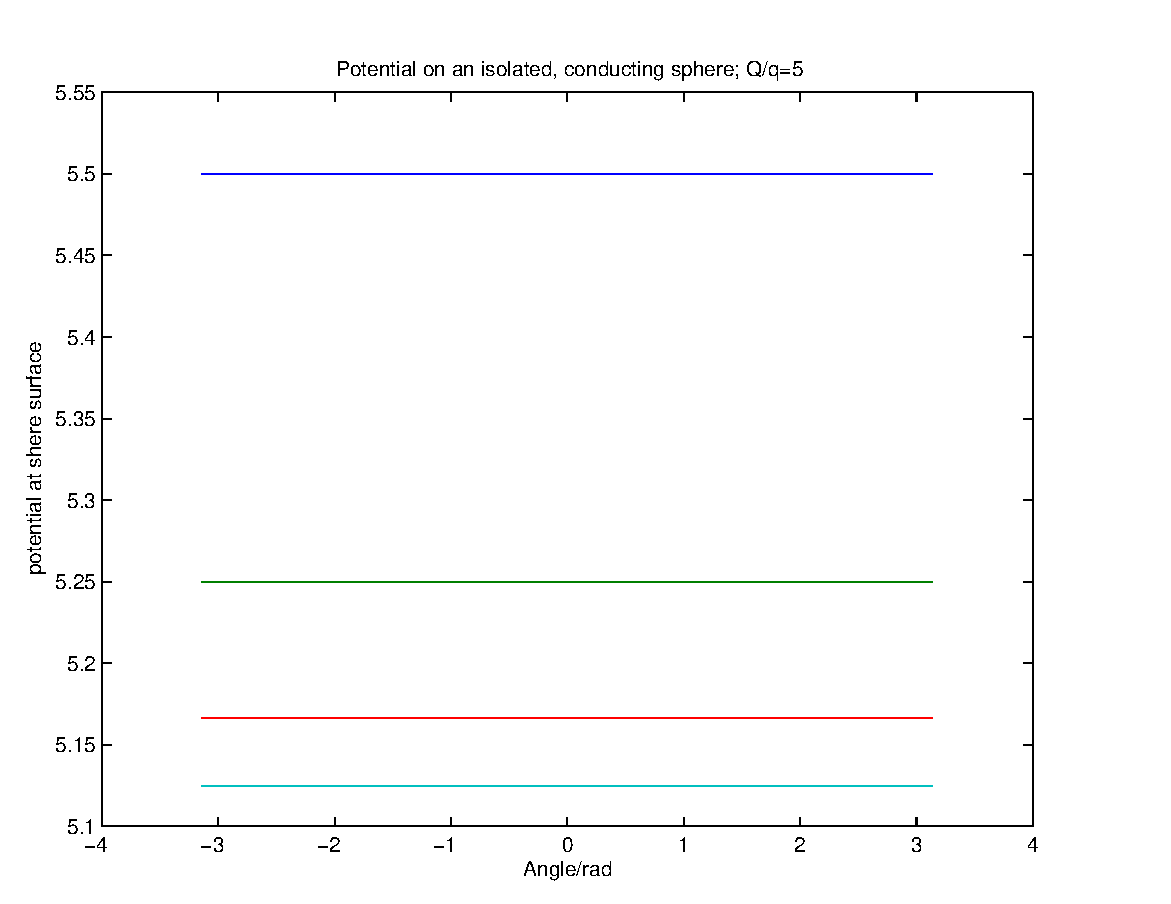
\includegraphics[width=12cm]{pics/potential_conduct_isolated_sphere.eps}\\
  \caption{Potential on the surface of an isolated conducting sphere, due to by a single charge}\label{fig_potential_conducd_isolated_sphere}
\end{figure}

\paragraph*{}
The surface charge distribution is now

\begin{eqnarray}
\sigma(\gamma)&=&-\frac{1}{4\pi}\mathbf{\hat{r}}\cdot \nabla \Phi(\mathbf{r}=a) \label{surface charge _chargenearisolatedsphere} \\
&=& -\frac{1}{4\pi}\mathbf{\hat{r}}\cdot \nabla \left[ \frac{q}{|\mathbf{r}-\mathbf{x}|} +\frac{q'}{|\mathbf{r}-\mathbf{x'}|} + \frac{Q+q \frac{a}{x}}{|\mathbf{r}|}\right] \nonumber
\\
&=& -\frac{1}{4\pi}\mathbf{\hat{r}}\cdot \nabla \left[ \frac{q}{|\mathbf{r}-\mathbf{x}|}-\frac{ \frac{a}{x} q}
{|\mathbf{r}- \frac{a^2}{x}\mathbf{\hat{x}}|} + \frac{Q+q \frac{a}{x}}{|\mathbf{r}|} \right] \nonumber
\\
&=& -\frac{q}{4\pi}\mathbf{\hat{r}}\cdot \nabla \left[ \frac{1}{|\mathbf{r}-\mathbf{x}|}-\frac{ \frac{a}{x} }
{|\mathbf{r}- \frac{a^2}{x}\mathbf{\hat{x}}|}+ \frac{\frac{Q}{q}+ \frac{a}{x}}{|\mathbf{r}|} \right] \nonumber
\\
&=& -\frac{q}{4\pi}\mathbf{\hat{r}}\cdot \left[ \frac{-(\mathbf{r}-\mathbf{x})}{|\mathbf{r}-\mathbf{x}|^3}-\frac{ -\frac{a}{x} (\mathbf{r}- \frac{a^2}{x}\mathbf{\hat{x}})}
{|\mathbf{r}- \frac{a^2}{x}\mathbf{\hat{x}}|^3} - \frac{\mathbf{r}(\frac{Q}{q}+ \frac{a}{x})}{|\mathbf{r}|^3}\right] \nonumber
\\
&=& \frac{q}{4\pi}\mathbf{\hat{r}}\cdot \left[ \frac{(\mathbf{r}-\mathbf{x})}{(r^2+x^2-2rx\cos \gamma)^\frac{3}{2}}-\frac{ \frac{a}{x} (\mathbf{r}- \frac{a^2}{x}\mathbf{\hat{x}})}
{(r^2+ \frac{a^4}{x^2} -2 \frac{ra^2}{x}\cos \gamma)^\frac{3}{2}} +\frac{\mathbf{r}(\frac{Q}{q}+ \frac{a}{x})}{r^3}\right] \nonumber
\\
&=& \frac{q}{4\pi} \left[ \frac{(r-x\cos \gamma)}{(r^2+x^2-2rx\cos \gamma)^\frac{3}{2}}-\frac{ \frac{a}{x} (r- \frac{a^2}{x}\cos \gamma)}
{(r^2+ \frac{a^4}{x^2} -2 \frac{ra^2}{x}\cos \gamma)^\frac{3}{2}} +\frac{\frac{Q}{q}+ \frac{a}{x}}{r^2}\right] \nonumber
\end{eqnarray}

\paragraph*{}
At $r=a$:

\begin{equation}
\sigma(\gamma)_{r=a}= \frac{q}{4\pi a^2} \left[ \frac{(1-\frac{x}{a}\cos \gamma)}{(1+\frac{x^2}{a^2}-2\frac{x}{a}\cos \gamma)^\frac{3}{2}}-\frac{ \frac{a}{x} (1- \frac{a}{x}\cos \gamma)}{(1+ \frac{a^2}{x^2} -2 \frac{a}{x}\cos \gamma)^\frac{3}{2}} + \frac{Q}{q}+ \frac{a}{x}\right]
\end{equation}

\begin{figure}
  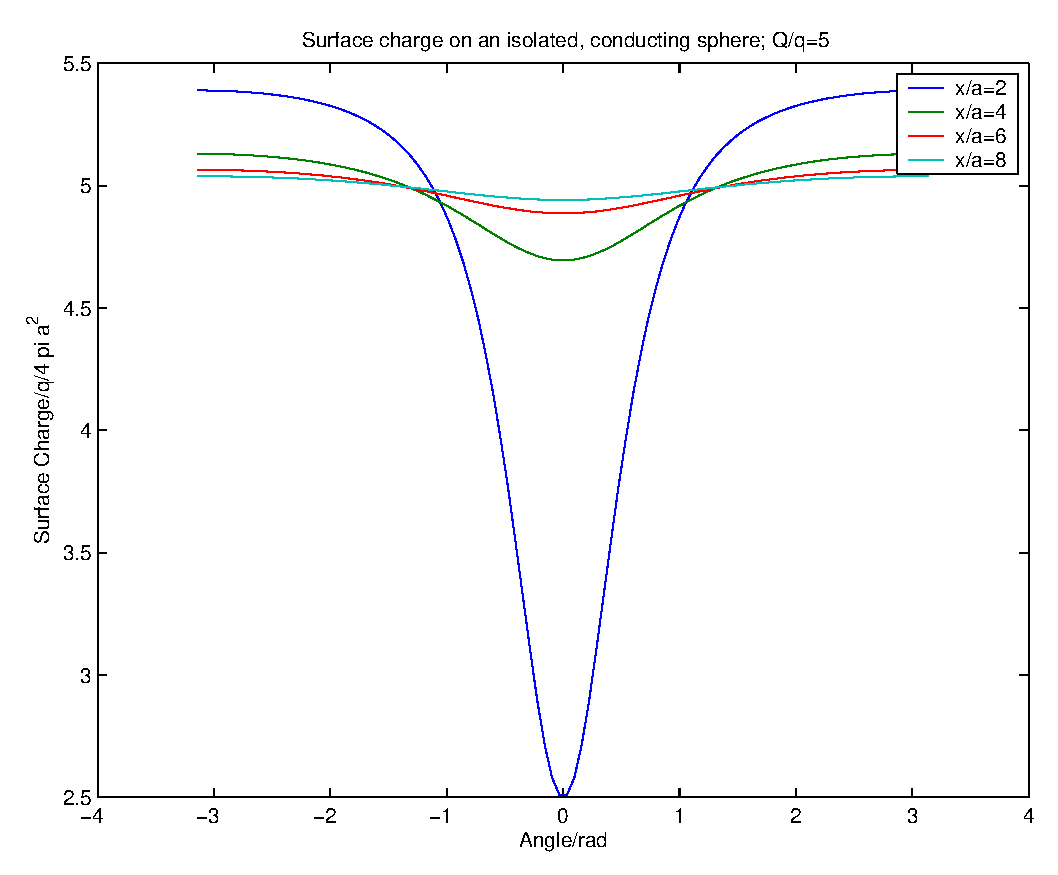
\includegraphics[width=12cm]{pics/surf_charge_conduct_isolated_sphere.eps}\\
  \caption{Surface charge, induced on an isolated conducting sphere by a single charge}\label{fig_surf_charge_conducd_isolated_sphere}
\end{figure}

\paragraph*{}
As can be seen in fig. \ref{fig_surf_charge_conducd_isolated_sphere}, the total charge on the sphere has to remain constant, just the distribution is changed. free charges (normally electrons) move to produce the correct field distribution, such as to minimize the potential energy of the system.

\subsection{The force}
\paragraph*{}
The force is now

\begin{eqnarray}\label{force_on_charge_conduct_isolated_sphere}
F(q,q',Q,\mathbf{x})&=& \frac{1}{4 \pi \varepsilon_0} \left[ \frac{qq' (\mathbf{x}-\mathbf{x'})}{|\mathbf{x}-\mathbf{x'}|^3} + \frac{\mathbf{x}qQ}{|\mathbf{x}|^3} \right]
\\
&=& \mathbf{\hat{x}}\frac{1}{4 \pi \varepsilon_0} \left[ \frac{qQ}{x^2} -\frac{q^2  \frac{a}{x} }{(x-x')^2} \right] \nonumber
\\
&=& \mathbf{\hat{x}}\frac{1}{4 \pi \varepsilon_0} \frac{q}{x^2}  \left[Q- \frac{qa}{x(1-\frac{a^2}{x^2})^2}\right] \nonumber
\end{eqnarray}


\paragraph*{}
When the charges Q and q have opposite values, the force on the charge is always is always towards the sphere. If the charges have the same sign, the force is only towards the sphere at a small distance from the surface. The unstable equilibrium is



\begin{eqnarray}
  F(q,q',Q,\mathbf{x}) &=& 0 \\
\Rightarrow  \frac{Q}{x^2}- \frac{qa}{x^3(1-\frac{a^2}{x^2})^2}&=& 0\\
Q- \frac{qa}{x(1-\frac{a^2}{x^2})^2}&=& 0\\
\frac{Q}{q}- \frac{a}{x(1-\frac{a^2}{x^2})^2}&=& 0
\end{eqnarray}

\paragraph*{}
Substituting $X=\frac{x}{a}$ and $Q'=\frac{Q}{q}$,

\begin{eqnarray}
Q'&=&\frac{1}{X(1-\frac{1}{X^2})^2}\\
X(1-\frac{1}{X^2})^2&=&\frac{1}{Q'}\\
X(1-2\frac{1}{X^2}+\frac{1}{X^4})&=&\frac{1}{Q'}\\
X-2\frac{1}{X}+\frac{1}{X^3}&=&\frac{1}{Q'}\\
X^4-\frac{X^3}{Q'}-2X^2+1&=&0\\
\end{eqnarray}

\begin{figure}
  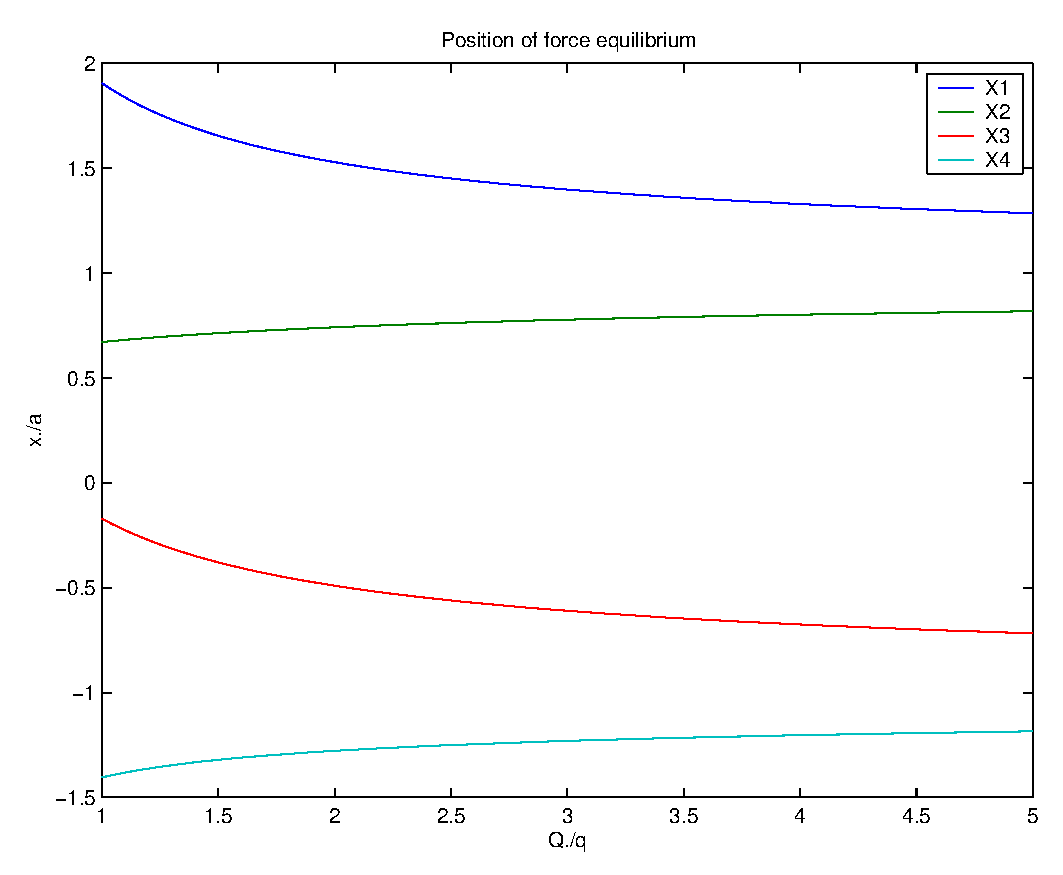
\includegraphics[width=12cm]{pics/EquilibriumPoint.eps}\\
  \caption{Position of the force equilibrium}\label{fig_force_equilibrium_conduct_isolated_sphere}
\end{figure}

\begin{figure}
  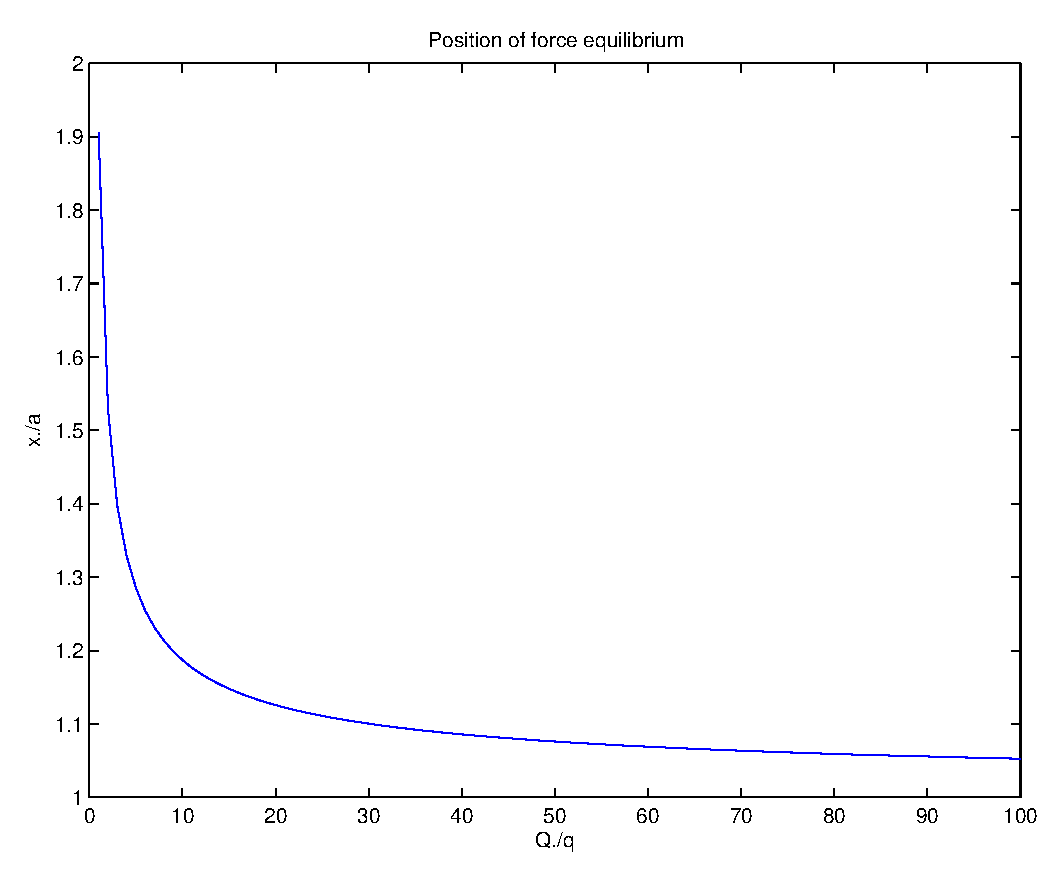
\includegraphics[width=12cm]{pics/EquilibriumPoint2.eps}\\
  \caption{Position of the force equilibrium}\label{fig_force_equilibrium_conduct_isolated_sphere_2}
\end{figure}
\paragraph*{}
This equation can easily be solved (see Fig. \ref{fig_force_equilibrium_conduct_isolated_sphere}). It has four solutions, but only the first makes physically sense. This solution is plotted for a larger range in figure \ref{fig_force_equilibrium_conduct_isolated_sphere_2}. As one can see, the equilibrium point quickly approaches the sphere, when $\frac{Q}{q}$ is large. For real situations, one would expect that the ratio is really large, so the layer where the force is attractive is very small. Since spacecraft normally accumulate negative charge, I would expect that the tendency to accumulate negative charge is increasing as a function of charge, since the positive ions are repelled, most of the time, while electrons are attracted all the time.



\paragraph*{}
In the limit of large distances ($x\gg a$), (\ref{force_on_charge_conduct_isolated_sphere}) this reduces to

\begin{equation}
F(q,q',\mathbf{x})|_{x \gg a}= \mathbf{\hat{x}}\frac{1}{4 \pi \varepsilon_0}  \left[ \frac{qQ}{x^2}  \right]
\end{equation}

\begin{figure}
  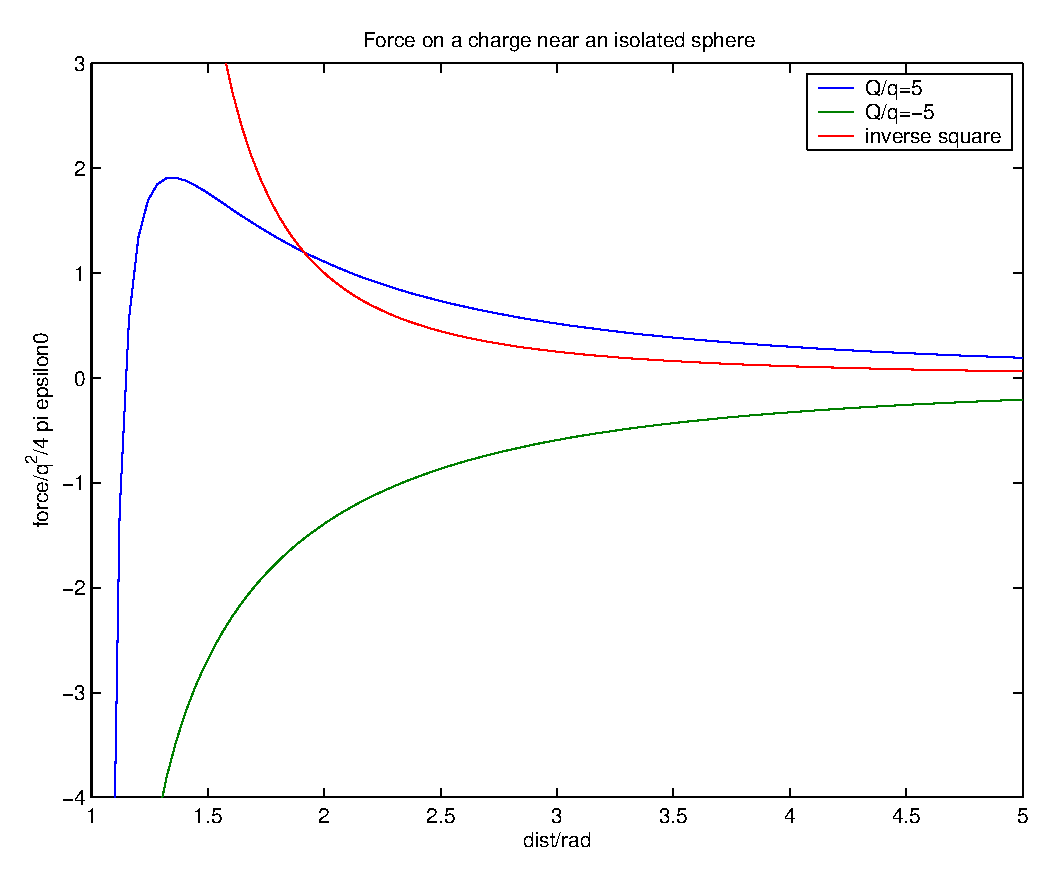
\includegraphics[width=12cm]{pics/force_on_charge_conduct_isolated_sphere.eps}\\
  \caption{Force on a charge near an isolated conducting sphere}\label{fig_force_on_charge_conduct_isolated_sphere}
\end{figure}

\paragraph*{}
which is the Coulomb law between two charges Q and q.

\section{A charge near a conducting, isolated sphere of charge Q, using the Debye potential}
\subsection{Deriving the Debye potential}


\paragraph*{}
In plasma, the observable potential due to a charge is smaller than in free space. The reason is the Debeye shielding effect. When a plasma is influenced by a potential, the distribution of the particles can be modeled by the Boltzmann factor $e^{-\frac{H}{k_bT}}$, where H is the Hamiltonian, and $k_b$ the Boltzmann constant. Hence, the number densities for ions and electrons are

\begin{eqnarray}
  n_i&=& n_0  e^{-\frac{e\Phi}{k_bT}} \\
n_e&=& n_0 e^{\frac{e\Phi}{k_bT}}
\end{eqnarray}

\paragraph*{}
The charge density is

\begin{eqnarray}
    \rho_e&=&e(n_i-n_e)\\
&=&en_0(e^{-\frac{e\Phi}{k_bT}} - e^{\frac{e\Phi}{k_bT}})\nonumber\\
&=&-en_0(e^{\frac{e\Phi}{k_bT}} - e^{\frac{-e\Phi}{k_bT}})\nonumber\\
&=&-2en_0\sinh\left(\frac{e\Phi}{k_bT}\right)\nonumber
\end{eqnarray}

\paragraph*{}
From

\begin{equation}\label{gradient_potential}
\mathbf{E}=-\nabla\Phi
\end{equation}

\paragraph*{}
we get

\begin{eqnarray}\label{poisson_equation}
  \nabla^2\Phi &=& -\frac{\rho_e}{\varepsilon_0} \\
&=&\frac{2en_0}{\varepsilon_0}\sinh\left(\frac{e\Phi}{k_bT}\right)\nonumber
\end{eqnarray}

\paragraph*{}
Since the electrostatic energy is supposed to be small in relation the the thermal energy of the electron, the sinh function can be approximated to the first order.

\begin{equation}\label{diff}
    \nabla^2\Phi=\frac{2e^2n_0\Phi}{k_bT\varepsilon_0}
\end{equation}

\paragraph*{}
We can define the Debye length $\lambda_D$ as

\begin{equation}\label{Debye_length}
    \lambda_D=\sqrt{\frac{k_bT\varepsilon_0}{2e^2n_0}}
\end{equation}

\paragraph*{}
Then

\begin{equation}\label{diff}
    \nabla^2\Phi=\frac{2}{\lambda_D^2}\Phi
\end{equation}

\paragraph*{}
The solution of (\ref{diff}) is

\begin{equation}\label{debye_potential}
    \Phi=\frac{1}{4 \pi \varepsilon_0}\frac{Q}{r}e^{-\frac{\sqrt{2}r}{\lambda_D}}
\end{equation}

\subsection{The Debye potential in cgs units}
\paragraph*{}
From (\ref{poisson_equation}):

\begin{eqnarray}
  \nabla^2\Phi &=& -4\pi\rho_e \\
&=&8 \pi en_0\sinh\left(\frac{e\Phi}{k_bT}\right)\nonumber
\end{eqnarray}

\paragraph*{}
Since the electrostatic energy is supposed to be small in relation the the thermal energy of the electron, the sinh function can be approximated to the first order.

\begin{equation}\label{diff_cgs}
    \nabla^2\Phi=\frac{8 \pi e^2n_0\Phi}{k_bT}
\end{equation}

\paragraph*{}
We can define the Debye length $\lambda_D$ as

\begin{equation}\label{Debye_length2}
    \lambda_D=\sqrt{\frac{k_bT}{4 \pi e^2n_0}}
\end{equation}

\paragraph*{}
Then

\begin{equation}\label{diff2}
    \nabla^2\Phi=\frac{2}{\lambda_D^2}\Phi
\end{equation}

\paragraph*{}
The solution of (\ref{diff2}) is

\begin{equation}\label{debye_potential}
    \Phi=\frac{Q}{r}e^{-\frac{\sqrt{2}r}{\lambda_D}}
\end{equation}


\begin{figure}
  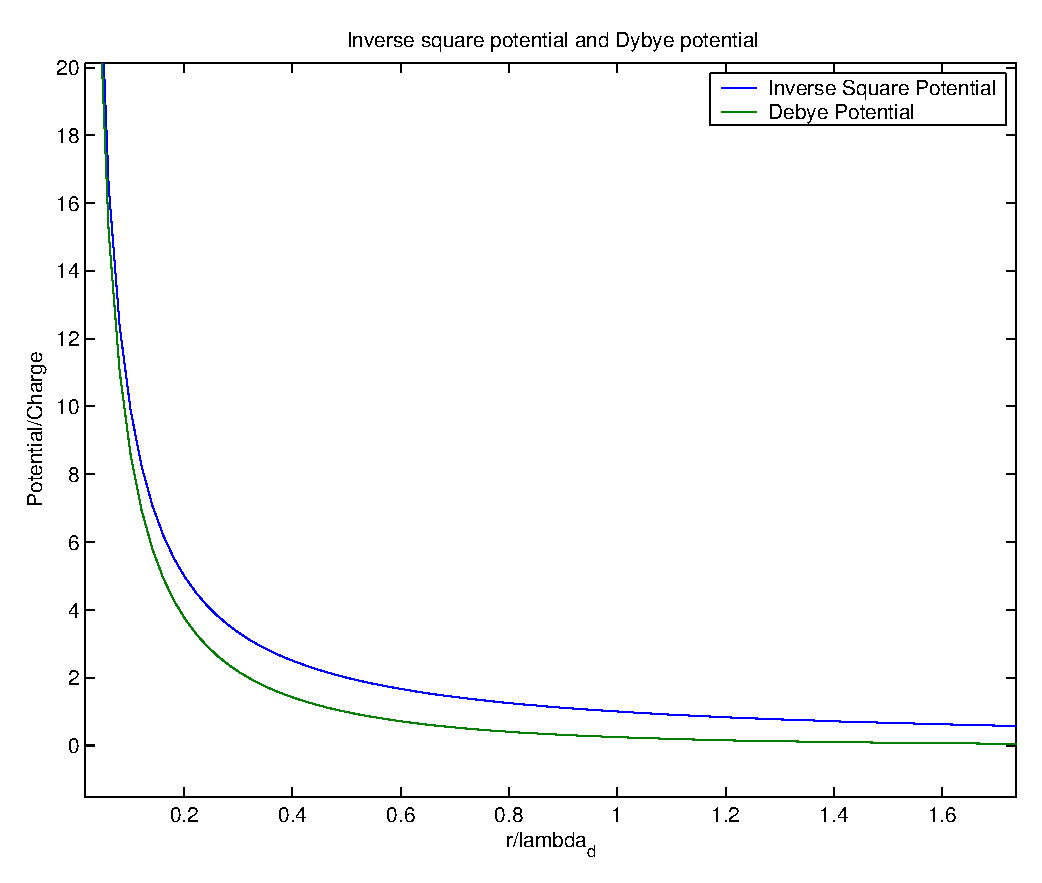
\includegraphics[width=12cm]{pics/debye_potential.eps}\\
  \caption{Inverse square potential vs. Debye potential}\label{fig_debye_potential}
\end{figure}

\paragraph*{}
Figure \ref{fig_debye_potential} shows the relation between normal inverse square potential and Debye potential, which is falling off more quickly.

\subsection{The charge distribution}
\paragraph*{}
The potential has to be modified to include the exponential factor. The effect of the plasma on the potential of the charge of the sphere acts only outside the sphere, since inside there is no plasma. This forms the exponential of the third exponential term. Additionally, since the effect of the plasma on the potential of the image charge has to be the same as on the potential of the charge, I use the same term in the exponential function. this reproduces the correct boundary conditions on the surface of the sphere. As there can be seen in Figure \ref{fig_potential_conducd_isolated_sphere}, the potential on the surface of the sphere is the same as without shielding plasma.

\paragraph*{}
This seems to be an ad hoc solution which is only true for the surface. in general, the charge and position of the image charge has to be chosen in a way that the potential add up to zero on the surface of the sphere. At the moment I can not find a solution to the resulting equation:

\begin{equation}\label{bedingung_image charge}
\frac{q}{|\mathbf{a}-\mathbf{x}|}e^{-\frac{\sqrt{2}|\mathbf{a}-\mathbf{x}|}{\lambda_D}}=\frac{q'}{|\mathbf{a}-\mathbf{x'}|}e^{-\frac{\sqrt{2}|\mathbf{a}-\mathbf{x'}|}{\lambda_D}}
\end{equation}

\begin{equation}\label{debye_potential_chargenearisolatedsphere} \Phi(\mathbf{r})=\frac{q}{|\mathbf{r}-\mathbf{x}|}e^{-\frac{\sqrt{2}|\mathbf{r}-\mathbf{x}|}{\lambda_D}}- \frac{aq}{x|\mathbf{r}-\mathbf{\frac{a^2}{x^2}\mathbf{x}}|}e^{-\frac{\sqrt{2}|\mathbf{r}-\mathbf{x}|}{\lambda_D}}+\frac{Q+q \frac{a}{x}}{|\mathbf{r}|}e^{-\frac{\sqrt{2}(r-a\cdot \mathcal{H}(r-a))}{\lambda_D}}
\end{equation}

\paragraph*{}
$\mathcal{H}(r-a)$ is the heavy side step function. It can be constructed with use of the delta function:

\begin{equation}\label{step_function}
    \mathcal{H}(r-a)=\int_{-\infty}^x\delta (r-a) dx
\end{equation}

\paragraph*{}
Hence

\begin{equation}\label{debye_potential_chargenearisolatedsphere_2} \Phi(\mathbf{r})=\frac{q}{|\mathbf{r}-\mathbf{x}|}e^{-\frac{\sqrt{2}|\mathbf{r}-\mathbf{x}|}{\lambda_D}}- \frac{aq}{x|\mathbf{r}-\mathbf{\frac{a^2}{x^2}\mathbf{x}}|}e^{-\frac{\sqrt{2}|\mathbf{r}-\mathbf{x}|}{\lambda_D}}+\frac{Q+q \frac{a}{x}}{|\mathbf{r}|}e^{-\frac{\sqrt{2}(r- \int_{-\infty}^x a \delta (r-a) dx)}{\lambda_D}}
\end{equation}

\begin{figure}
  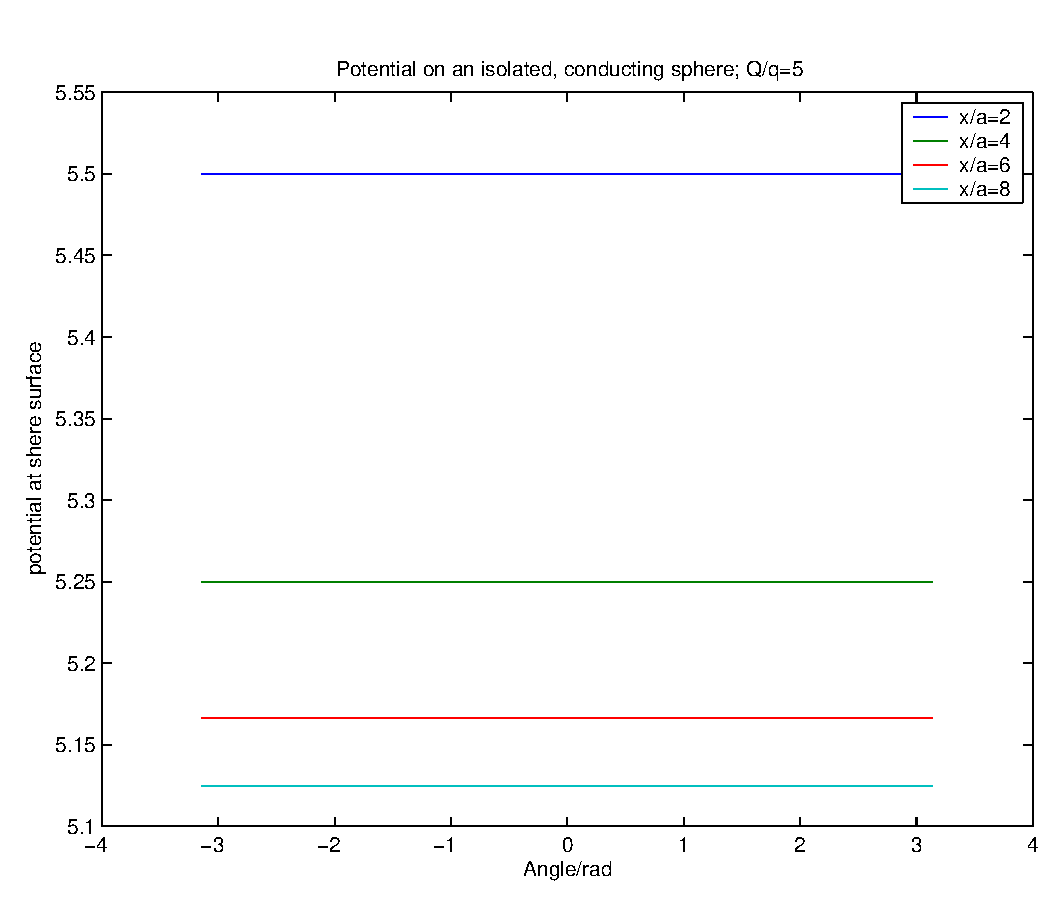
\includegraphics[width=12cm]{pics/potential_conduct_isolated_sphere_debye.eps}\\
  \caption{Potential on the surface of an isolated conducting sphere, due to by a single charge, using the Debye potential}\label{fig_potential_conducd_isolated_sphere}
\end{figure}
%------------------------ step function
\paragraph*{}
The surface charge distribution is now

\begin{eqnarray}
\sigma(\gamma)&=&-\frac{1}{4\pi}\mathbf{\hat{r}}\cdot \nabla \Phi(\mathbf{r}=a) \label{surface charge _chargenearisolatedsphere_debye_potential} \\
&=& -\frac{1}{4\pi}\mathbf{\hat{r}}\cdot \nabla \left[ \frac{q}{|\mathbf{r}-\mathbf{x}|}e^{-\frac{\sqrt{2}|\mathbf{r}-\mathbf{x}|}{\lambda_D}}-\frac{ \frac{a}{x} q}
{|\mathbf{r}- \frac{a^2}{x}\mathbf{\hat{x}}|}e^{-\frac{\sqrt{2}|\mathbf{r}-\mathbf{x}|}{\lambda_D}} + \frac{Q+q \frac{a}{x}}{|\mathbf{r}|}e^{-\frac{\sqrt{2}(r- \int_{-\infty}^x a \delta (r-a) dx)}{\lambda_D}} \right] \nonumber
\\
&=& -\frac{q}{4\pi}\mathbf{\hat{r}}\cdot \nabla \left[ \frac{1}{|\mathbf{r}-\mathbf{x}|}e^{-\frac{\sqrt{2}|\mathbf{r}-\mathbf{x}|}{\lambda_D}}-\frac{ \frac{a}{x}}
{|\mathbf{r}- \frac{a^2}{x}\mathbf{\hat{x}}|}e^{-\frac{\sqrt{2}|\mathbf{r}-\mathbf{x}|}{\lambda_D}} + \frac{\frac{Q}{q}+ \frac{a}{x}}{|\mathbf{r}|}e^{-\frac{\sqrt{2}(r- \int_{-\infty}^x a \delta (r-a) dx)}{\lambda_D}} \right] \nonumber
\end{eqnarray}

\paragraph*{}
The components:
\begin{eqnarray}
  \nabla \frac{1}{|\mathbf{r}-\mathbf{x}|}e^{-\frac{\sqrt{2}|\mathbf{r}-\mathbf{x}|}{\lambda_D}}&=& \frac{-(\mathbf{r}-\mathbf{x})}{|\mathbf{r}-\mathbf{x}|^3} e^{-\frac{\sqrt{2}|\mathbf{r}-\mathbf{x}|}{\lambda_D}} + \frac{1}{|\mathbf{r}-\mathbf{x}|} e^{-\frac{\sqrt{2}|\mathbf{r}-\mathbf{x}|}{\lambda_D}} \cdot -\frac{\sqrt{2}\left( \mathbf{r}-\mathbf{x}\right)}{\lambda_D |\mathbf{r}-\mathbf{x}|}\\
 &=&-e^{-\frac{\sqrt{2}|\mathbf{r}-\mathbf{x}|}{\lambda_D}} (\mathbf{r}-\mathbf{x})\left[ \frac{1}{|\mathbf{r}-\mathbf{x}|^3}  + \frac{1}{|\mathbf{r}-\mathbf{x}|^2}  \frac{\sqrt{2}}{\lambda_D}\right]\nonumber
 \end{eqnarray}

\begin{eqnarray}
  \nabla \frac{ \frac{a}{x}}
{|\mathbf{r}- \frac{a^2}{x}\mathbf{\hat{x}}|}e^{-\frac{\sqrt{2}|\mathbf{r}-\mathbf{\frac{a^2}
{x^2}\mathbf{x}}|}{\lambda_D}}
&=& \frac{-\frac{a}{x}(\mathbf{r}- \frac{a^2}{x}\mathbf{\hat{x}})}{|\mathbf{r}- \frac{a^2}{x}\mathbf{\hat{x}}|^3} e^{-\frac{\sqrt{2}|\mathbf{r}- \frac{a^2}{x}\mathbf{\hat{x}}|}{\lambda_D}} + \frac{a}{x}\frac{1}{|\mathbf{r}- \frac{a^2}{x}\mathbf{\hat{x}}|} e^{-\frac{\sqrt{2}|\mathbf{r}- \frac{a^2}{x}\mathbf{\hat{x}}|}{\lambda_D}} \cdot -\frac{\sqrt{2}\left( \mathbf{r}- \frac{a^2}{x}\mathbf{\hat{x}}\right)}{\lambda_D |\mathbf{r}- \frac{a^2}{x}\mathbf{\hat{x}}|}\\
 &=&-\frac{a}{x}e^{-\frac{\sqrt{2}|\mathbf{r}- \frac{a^2}{x}\mathbf{\hat{x}}|}{\lambda_D}}\left( \mathbf{r}- \frac{a^2}{x}\mathbf{\hat{x}}\right) \left[ \frac{1}{|\mathbf{r}- \frac{a^2}{x}\mathbf{\hat{x}}|^3}  + \frac{1}{|\mathbf{r}- \frac{a^2}{x}\mathbf{\hat{x}}|^2}  \frac{\sqrt{2}}{\lambda_D}\right]\nonumber
 \end{eqnarray}

\begin{eqnarray}
   \nabla \frac{\frac{Q}{q}+ \frac{a}{x}}{|\mathbf{r}|}e^{-\frac{\sqrt{2}r}{\lambda_D}}
   &=& -\frac{(\frac{Q}{q}+ \frac{a}{x})\mathbf{r}}{|\mathbf{r}|^3}e^{-\frac{\sqrt{2}r}{\lambda_D}}
   -\frac{\frac{Q}{q}+ \frac{a}{x}}{|\mathbf{r}|^2}e^{-\frac{\sqrt{2}r}{\lambda_D}}\frac{\sqrt{2}}{\lambda_D}\mathbf{r}\\
 &=& -e^{-\frac{\sqrt{2}r}{\lambda_D}}\left(\frac{Q}{q}+ \frac{a}{x}\right)\mathbf{r}\left[ \frac{1}{|\mathbf{r}|^3}
   +\frac{1}{|\mathbf{r}|^2}\frac{\sqrt{2}}{\lambda_D}\right] \nonumber
 \end{eqnarray}

\paragraph*{}
Further:

\begin{eqnarray}
  \mathbf{\hat{r}}\cdot \nabla \frac{1}{|\mathbf{r}-\mathbf{x}|}e^{-\frac{\sqrt{2}|\mathbf{r}-\mathbf{x}|}{\lambda_D}}&=& -e^{-\frac{\sqrt{2}|\mathbf{r}-\mathbf{x}|}{\lambda_D}} \mathbf{\hat{r}}\cdot(\mathbf{r}-\mathbf{x})\left[ \frac{1}{|\mathbf{r}-\mathbf{x}|^3}  + \frac{1}{|\mathbf{r}-\mathbf{x}|^2}  \frac{\sqrt{2}}{\lambda_D}\right]
\\ &=&
-e^{-\frac{\sqrt{2}|\mathbf{r}-\mathbf{x}|}{\lambda_D}} (|\mathbf{r}|-|\mathbf{x}|\cos \gamma)\left[ \frac{1}{|\mathbf{r}-\mathbf{x}|^3}  + \frac{1}{|\mathbf{r}-\mathbf{x}|^2}  \frac{\sqrt{2}}{\lambda_D}\right]\nonumber \\ &=&
-e^{-\frac{\sqrt{2(r^2+x^2-2rx \cos \gamma)}}{\lambda_D}} (r-x\cos \gamma)\nonumber \\
&\times&\left[ \frac{1}{(r^2+x^2-2rx \cos \gamma)^{\frac{3}{2}}}
+ \frac{1}{(r^2+x^2-2rx \cos \gamma)}  \frac{\sqrt{2}}{\lambda_D}\right]\nonumber
\end{eqnarray}

\begin{eqnarray}
 \mathbf{\hat{r}}\cdot \nabla \frac{ \frac{a}{x}}
{|\mathbf{r}- \frac{a^2}{x}\mathbf{\hat{x}}|}e^{-\frac{\sqrt{2}|\mathbf{r}-\mathbf{\frac{a^2}
{x^2}\mathbf{x}}|}{\lambda_D}}
&=& -\frac{a}{x}e^{-\frac{\sqrt{2}|\mathbf{r}- \frac{a^2}{x}\mathbf{\hat{x}}|}{\lambda_D}} \mathbf{\hat{r}}\cdot \left( \mathbf{r}- \frac{a^2}{x}\mathbf{\hat{x}}\right) \left[ \frac{1}{|\mathbf{r}- \frac{a^2}{x}\mathbf{\hat{x}}|^3}  + \frac{1}{|\mathbf{r}- \frac{a^2}{x}\mathbf{\hat{x}}|^2}  \frac{\sqrt{2}}{\lambda_D}\right]
\\ &=&
 -\frac{a}{x}e^{-\frac{\sqrt{2}|\mathbf{r}- \frac{a^2}{x}\mathbf{\hat{x}}|}{\lambda_D}} \left( |\mathbf{r}|- \frac{a^2}{x}\cos \gamma\right) \left[ \frac{1}{|\mathbf{r}- \frac{a^2}{x}\mathbf{\hat{x}}|^3}  + \frac{1}{|\mathbf{r}- \frac{a^2}{x}\mathbf{\hat{x}}|^2}  \frac{\sqrt{2}}{\lambda_D}\right] \nonumber
\\ &=&
 -\frac{a}{x}e^{-\frac{\sqrt{2(r^2 + \frac{a^4}{x^2}- 2r\frac{a^2}{x}\cos \gamma)}}{\lambda_D}} \left( r- \frac{a^2}{x}\cos \gamma\right) \nonumber \\
&\times & \left[ \frac{1}{(r^2 + \frac{a^4}{x^2}- 2r\frac{a^2}{x}\cos \gamma)^\frac{3}{2}}  + \frac{1}{(r^2 + \frac{a^4}{x^2}- 2r\frac{a^2}{x}\cos \gamma)}  \frac{\sqrt{2}}{\lambda_D}\right] \nonumber
 \end{eqnarray}

\begin{eqnarray}
   \mathbf{\hat{r}}\cdot \nabla \frac{\frac{Q}{q}+ \frac{a}{x}}{|\mathbf{r}|}e^{-\frac{\sqrt{2}(r-a)}{\lambda_D}}
   &=& -e^{-\frac{\sqrt{2}r}{\lambda_D}}\left(\frac{Q}{q}+ \frac{a}{x}\right)\mathbf{\hat{r}}\cdot\mathbf{r}\left[ \frac{1}{|\mathbf{r}|^3}+\frac{1}{|\mathbf{r}|^2}\frac{\sqrt{2}}{\lambda_D}\right]
\\ &=&
-e^{-\frac{\sqrt{2}r}{\lambda_D}}\left(\frac{Q}{q}+ \frac{a}{x}\right) |\mathbf{r}|\left[ \frac{1}{|\mathbf{r}|^3}
   +\frac{1}{|\mathbf{r}|^2}\frac{\sqrt{2}}{\lambda_D}\right] \nonumber
\\
&=&
-e^{-\frac{\sqrt{2}r}{\lambda_D}}\left(\frac{Q}{q}+ \frac{a}{x}\right) \left[ \frac{1}{r^2}
   +\frac{1}{r}\frac{\sqrt{2}}{\lambda_D}\right] \nonumber
 \end{eqnarray}



\paragraph*{}
At $r=a$:

\begin{eqnarray}
  \left[ \mathbf{\hat{r}}\cdot \nabla \frac{1}{|\mathbf{r}-\mathbf{x}|}e^{-\frac{\sqrt{2}|\mathbf{r}-\mathbf{x}|}{\lambda_D}}\right]_{r=a}&=& -e^{-\frac{\sqrt{2(a^2+x^2-2ax \cos \gamma)}}{\lambda_D}} (a-x\cos \gamma) \\
&\times&\left[ \frac{1}{(a^2+x^2-2ax \cos \gamma)^{\frac{3}{2}}}
+ \frac{1}{(a^2+x^2-2ax \cos \gamma)}  \frac{\sqrt{2}}{\lambda_D}\right]\nonumber
\\ &=&
-\frac{1}{a^2}e^{-\frac{a\sqrt{2(1+\frac{x^2}{a^2}-2\frac{x}{a} \cos \gamma)}}{\lambda_D}} (1-\frac{x}{a}\cos \gamma) \nonumber \\
&\times&\left[ \frac{1}{(1+\frac{x^2}{a^2}-2\frac{x}{a} \cos \gamma)^{\frac{3}{2}}}
+ \frac{a}{(1+\frac{x^2}{a^2}-2\frac{x}{a} \cos \gamma)}  \frac{\sqrt{2}}{\lambda_D}\right]\nonumber
\nonumber
\end{eqnarray}



\begin{eqnarray}
 \left[\mathbf{\hat{r}}\cdot \nabla \frac{ \frac{a}{x}}
{|\mathbf{r}- \frac{a^2}{x}\mathbf{\hat{x}}|}e^{-\frac{\sqrt{2}|\mathbf{r}-\mathbf{\frac{a^2}
{x^2}\mathbf{x}}|}{\lambda_D}}\right]_{r=a}
&=&-\frac{a}{x}e^{-\frac{\sqrt{2(2 a^2- 2\frac{a^3}{x}\cos \gamma)}}{\lambda_D}} \left( a- \frac{a^2}{x}\cos \gamma\right)  \\
&\times & \left[ \frac{1}{(2 a^2 - 2\frac{a^3}{x}\cos \gamma)^\frac{3}{2}}  + \frac{1}{(2 a^2- 2\frac{a^3}{x}\cos \gamma)}  \frac{\sqrt{2}}{\lambda_D}\right]\nonumber
\\ &=& -\frac{a}{x}e^{-\frac{2a\sqrt{( 1- \frac{a}{x}\cos \gamma)}}{\lambda_D}} a\left( 1- \frac{a}{x}\cos \gamma\right)  \nonumber \\
&\times & \left[ \frac{1}{a^3(2  - 2\frac{a}{x}\cos \gamma)^\frac{3}{2}}  + \frac{1}{2a^2(1 - \frac{a}{x}\cos \gamma)}  \frac{\sqrt{2}}{\lambda_D}\right]\nonumber
\\
&=& -\frac{1}{a^2}\frac{a}{x}e^{-\frac{2a\sqrt{( 1- \frac{a}{x}\cos \gamma)}}{\lambda_D}} \left( 1- \frac{a}{x}\cos \gamma\right)  \nonumber \\
&\times & \left[ \frac{1}{(2  - 2\frac{a}{x}\cos \gamma)^\frac{3}{2}}  + \frac{a}{(1 - \frac{a}{x}\cos \gamma)}  \frac{1}{\sqrt{2} \lambda_D}\right]\nonumber
 \end{eqnarray}


\begin{eqnarray}
   \left[\mathbf{\hat{r}}\cdot \nabla \frac{\frac{Q}{q}+ \frac{a}{x}}{|\mathbf{r}|}e^{-\frac{\sqrt{2}r}{\lambda_D}}\right]_{r=a}
   &=& e^{-\frac{\sqrt{2}a}{\lambda_D}}\left(\frac{Q}{q}+ \frac{a}{x}\right) \left[ \frac{1}{a^2}
   +\frac{1}{a}\frac{\sqrt{2}}{\lambda_D}\right]
 \end{eqnarray}


\paragraph*{}
Defining the Symbols \emph{A}, \emph{B} and \emph{C} for the three contributions to the surface charge density distribution, we can write down the total distribution as follows:

\begin{eqnarray}
\sigma(\gamma)_{r=a}&=& -\frac{q}{4\pi}\left[ -\mathcal{A} + \mathcal{B} - \mathcal{C}\right] \\
&=& \frac{q}{4\pi}\left[  \mathcal{A} - \mathcal{B} + \mathcal{C}\right] \nonumber
\end{eqnarray}

\paragraph*{}
where

\begin{eqnarray}
% \nonumber to remove numbering (before each equation)
  \mathcal{A} &=& \frac{1}{a^2}e^{-\frac{a\sqrt{2(1+\frac{x^2}{a^2}-2\frac{x}{a} \cos \gamma)}}{\lambda_D}} (1-\frac{x}{a}\cos \gamma) \nonumber \\
&\times&\left[ \frac{1}{(1+\frac{x^2}{a^2}-2\frac{x}{a} \cos \gamma)^{\frac{3}{2}}}
+ \frac{a}{(1+\frac{x^2}{a^2}-2\frac{x}{a} \cos \gamma)}  \frac{\sqrt{2}}{\lambda_D}\right]\nonumber
\nonumber \\
\mathcal{B} &=& \frac{1}{a^2}\frac{a}{x}e^{-\frac{2a\sqrt{( 1- \frac{a}{x}\cos \gamma)}}{\lambda_D}} \left( 1- \frac{a}{x}\cos \gamma\right)  \nonumber \\
&\times & \left[ \frac{1}{(2  - 2\frac{a}{x}\cos \gamma)^\frac{3}{2}}  + \frac{a}{(1 - \frac{a}{x}\cos \gamma)}  \frac{1}{\sqrt{2} \lambda_D}\right]\nonumber \\
\mathcal{C} &=& e^{-\frac{\sqrt{2}a}{\lambda_D}}\left(\frac{Q}{q}+ \frac{a}{x}\right) \left[ \frac{1}{a^2}
   +\frac{1}{a}\frac{\sqrt{2}}{\lambda_D}\right]\end{eqnarray}


\begin{figure}
  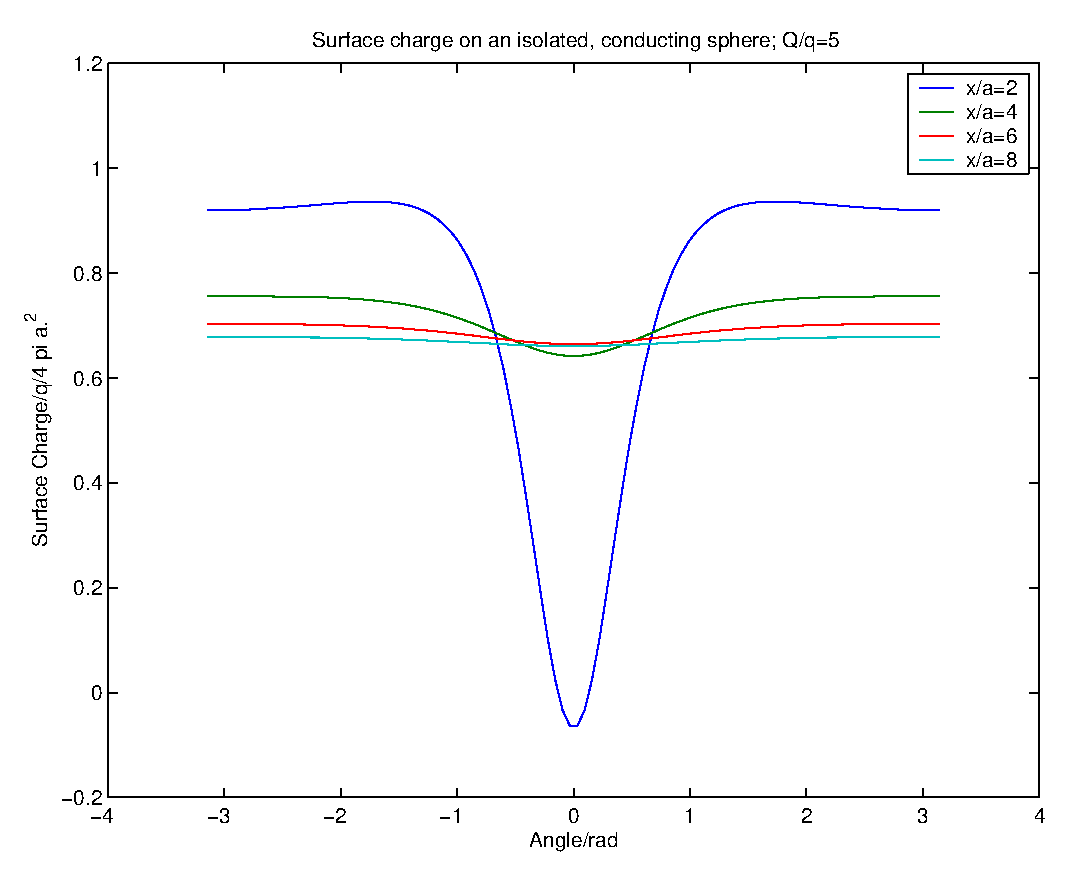
\includegraphics[width=12cm]{pics/surf_charge_conduct_isolated_sphere_debye.eps}\\
  \caption{Surface charge, induced on an isolated conducting sphere by a single charge, using the Debye Potential}\label{fig_surf_charge_conducd_isolated_sphere_decye}
\end{figure}

// binda---------------------------------------------------------------------------------------------
\paragraph*{}
As can be seen in fig. \ref{fig_surf_charge_conducd_isolated_sphere_debye}, the total charge on the sphere has to remain constant, just the distribution is changed. free charges (normally electrons) move to produce the correct field distribution, such as to minimize the potential energy of the system.

\subsection{The force}
\paragraph*{}
The force is now

\begin{eqnarray}\label{force_on_charge_conduct_isolated_sphere}
F(q,q',Q,\mathbf{x})&=& \frac{1}{4 \pi \varepsilon_0} \left[ \frac{qq' (\mathbf{x}-\mathbf{x'})}{|\mathbf{x}-\mathbf{x'}|^3} + \frac{\mathbf{x}qQ}{|\mathbf{x}|^3} \right]
\\
&=& \mathbf{\hat{x}}\frac{1}{4 \pi \varepsilon_0} \left[ \frac{qQ}{x^2} -\frac{q^2  \frac{a}{x} }{(x-x')^2} \right] \nonumber
\\
&=& \mathbf{\hat{x}}\frac{1}{4 \pi \varepsilon_0} \frac{q}{x^2}  \left[Q- \frac{qa}{x(1-\frac{a^2}{x^2})^2}\right] \nonumber
\end{eqnarray}


\paragraph*{}
When the charges Q and q have opposite values, the force on the charge is always is always towards the sphere. If the charges have the same sign, the force is only towards the sphere at a small distance from the surface. The unstable equilibrium is



\begin{eqnarray}
  F(q,q',Q,\mathbf{x}) &=& 0 \\
\Rightarrow  \frac{Q}{x^2}- \frac{qa}{x^3(1-\frac{a^2}{x^2})^2}&=& 0\\
Q- \frac{qa}{x(1-\frac{a^2}{x^2})^2}&=& 0\\
\frac{Q}{q}- \frac{a}{x(1-\frac{a^2}{x^2})^2}&=& 0
\end{eqnarray}

\paragraph*{}
Substituting $X=\frac{x}{a}$ and $Q'=\frac{Q}{q}$,

\begin{eqnarray}
Q'&=&\frac{1}{X(1-\frac{1}{X^2})^2}\\
X(1-\frac{1}{X^2})^2&=&\frac{1}{Q'}\\
X(1-2\frac{1}{X^2}+\frac{1}{X^4})&=&\frac{1}{Q'}\\
X-2\frac{1}{X}+\frac{1}{X^3}&=&\frac{1}{Q'}\\
X^4-\frac{X^3}{Q'}-2X^2+1&=&0\\
\end{eqnarray}

\begin{figure}
  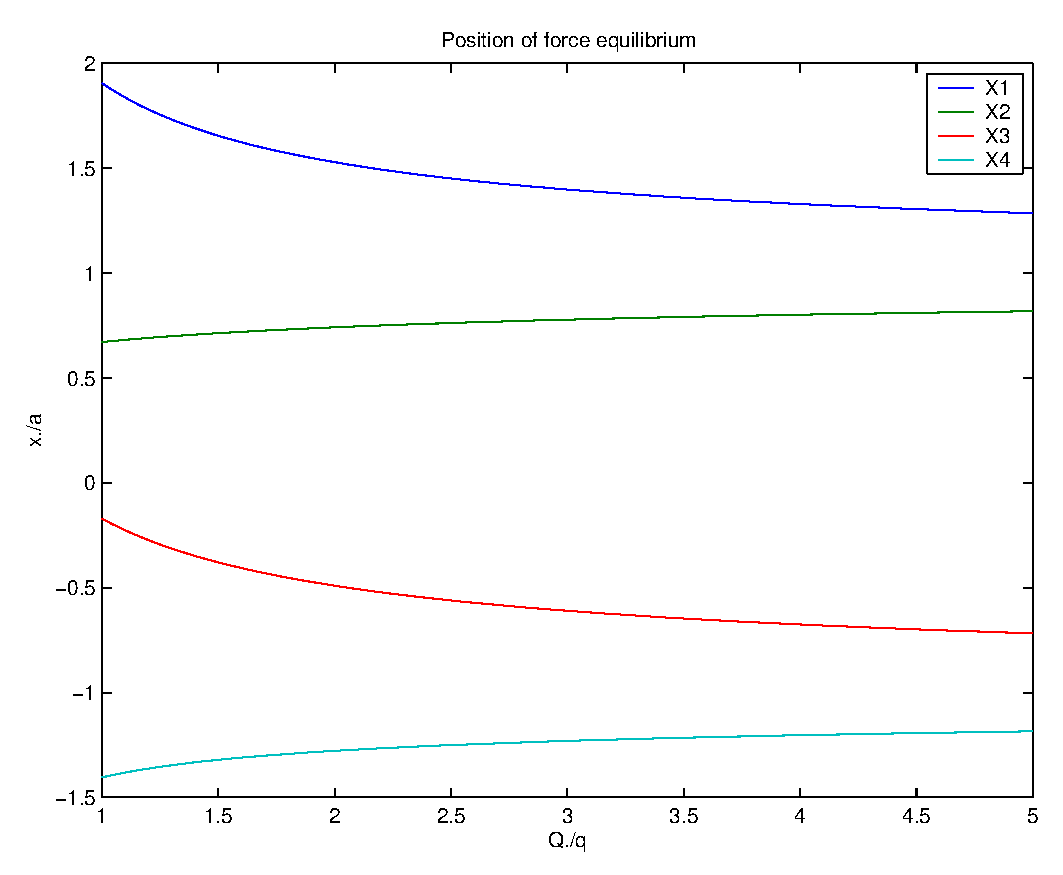
\includegraphics[width=12cm]{pics/EquilibriumPoint.eps}\\
  \caption{Position of the force equilibrium}\label{fig_force_equilibrium_conduct_isolated_sphere}
\end{figure}

\begin{figure}
  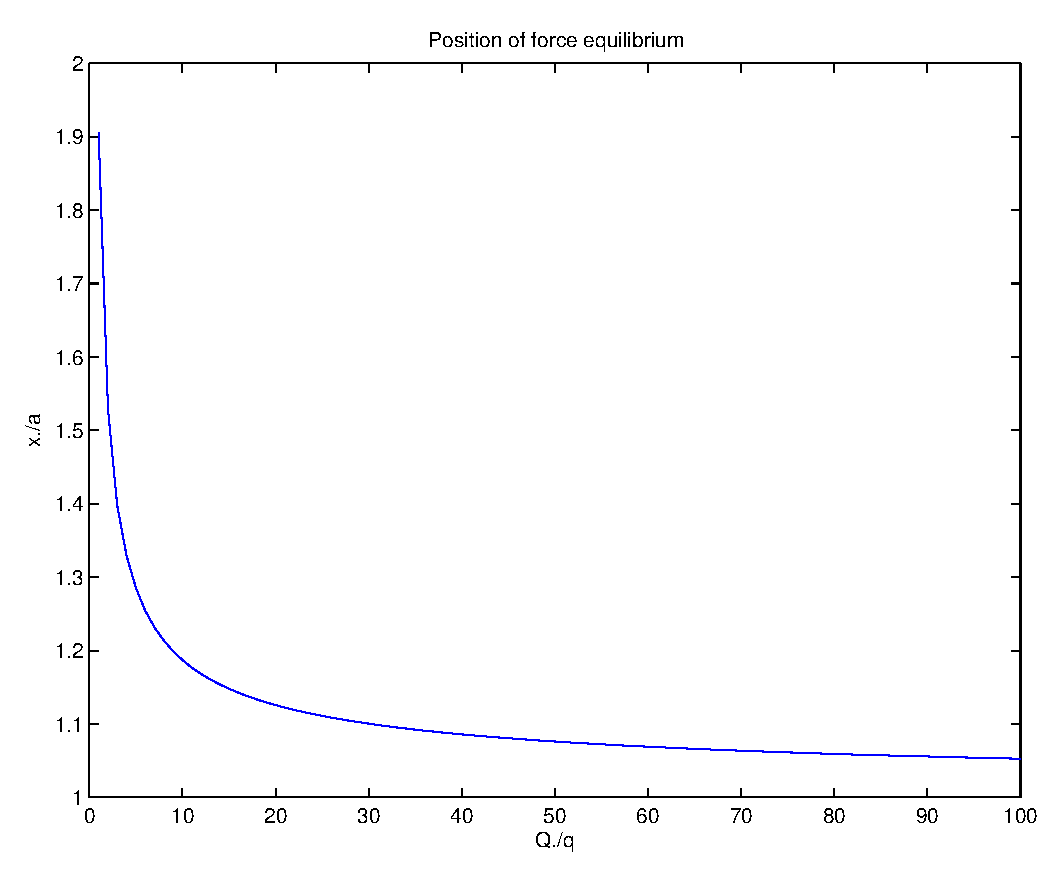
\includegraphics[width=12cm]{pics/EquilibriumPoint2.eps}\\
  \caption{Position of the force equilibrium}\label{fig_force_equilibrium_conduct_isolated_sphere_2}
\end{figure}
\paragraph*{}
This equation can easily be solved (see Fig. \ref{fig_force_equilibrium_conduct_isolated_sphere}). It has four solutions, but only the first makes physically sense. This solution is plotted for a larger range in figure \ref{fig_force_equilibrium_conduct_isolated_sphere_2}. As one can see, the equilibrium point quickly approaches the sphere, when $\frac{Q}{q}$ is large. For real situations, one would expect that the ratio is really large, so the layer where the force is attractive is very small. Since spacecraft normally accumulate negative charge, I would expect that the tendency to accumulate negative charge is increasing as a function of charge, since the positive ions are repelled, most of the time, while electrons are attracted all the time.



\paragraph*{}
In the limit of large distances ($x\gg a$), (\ref{force_on_charge_conduct_isolated_sphere}) this reduces to

\begin{equation}
F(q,q',\mathbf{x})|_{x \gg a}= \mathbf{\hat{x}}\frac{1}{4 \pi \varepsilon_0}  \left[ \frac{qQ}{x^2}  \right]
\end{equation}

\begin{figure}
  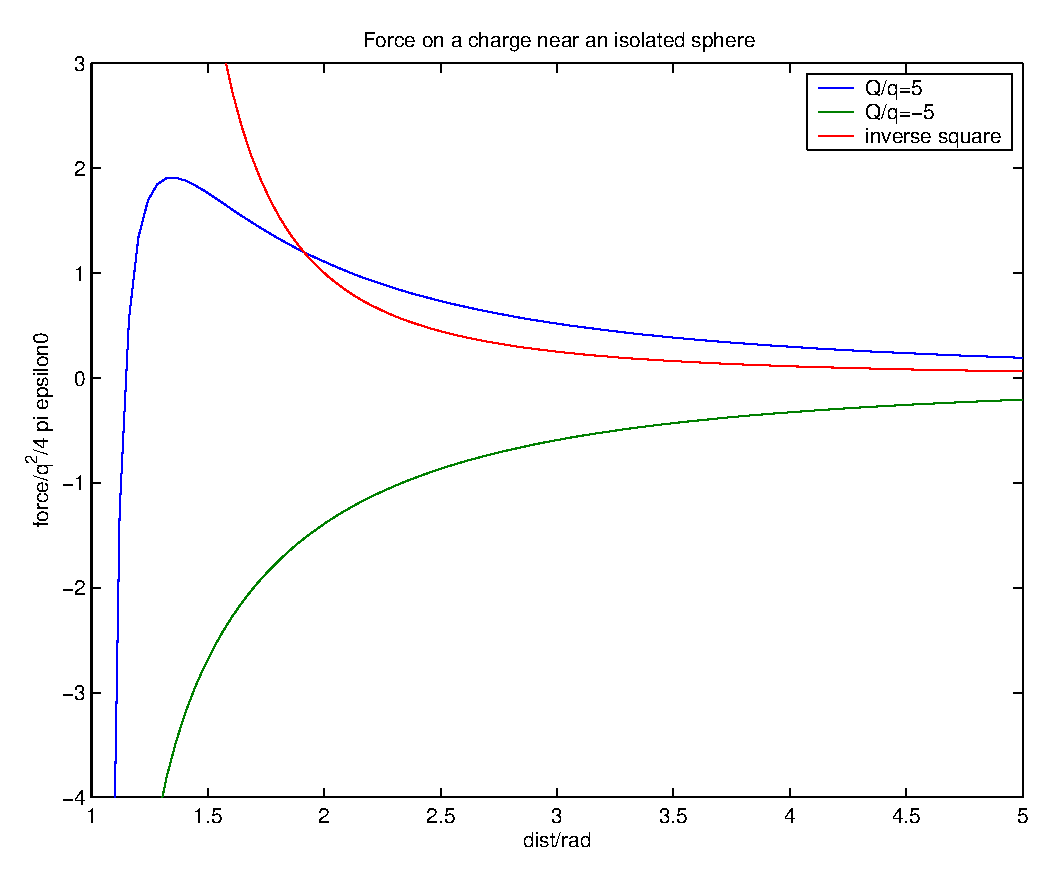
\includegraphics[width=12cm]{pics/force_on_charge_conduct_isolated_sphere.eps}\\
  \caption{Force on a charge near an isolated conducting sphere}\label{fig_force_on_charge_conduct_isolated_sphere}
\end{figure}

\paragraph*{}
which is the Coulomb law between two charges Q and q.


\chapter{Particle speed due to EM wave}
\section{Ignoring the magnetic field}
\paragraph*{}
Neglecting a magnetic field, the equation of motion of a particle pushed by a harmonic EM wave is

\begin{eqnarray}
F_e=m_e\frac{d^2\mathbf{r}}{dt^2}&=&q\mathbf{E}\label{force_on e} \\
\Rightarrow \frac{d^2\mathbf{r}}{dt^2}&=&\frac{q \mathbf{E}_0}{m} e^{i(\mathbf{k \cdot r}-\omega t)}
\end{eqnarray}

\paragraph*{}
Integrating yields


\begin{eqnarray}
\frac{\partial \mathbf{r}}{\partial t}&=&\frac{q \mathbf{E}_0}{i \omega m} e^{i(\mathbf{k \cdot r}-\omega t)}\label{solution_for_r_dot} \\
&=&\frac{q }{i \omega m} \mathbf{E}
\end{eqnarray}

\paragraph*{}
So the maximum speed is

\begin{equation}\label{max_particle_speed}
    \mathbf{v}_{max}=\frac{q }{ \omega m} \mathbf{E}_0
\end{equation}

\paragraph*{}
For electrons and radiation in the low frequency range, speeds can be relativistic, when fields are high.

\section{Including the magnetic field}
\subsection{the full equations}
\paragraph*{}
The new equation of motion

\begin{eqnarray}
F_e=m_e\frac{d^2\mathbf{r}}{dt^2}&=&q(\mathbf{E}+(\mathbf{v}\times \mathbf{B}))\label{force_on e_withB} \\
\Rightarrow \frac{d^2\mathbf{r}}{dt^2}&=&\frac{q }{m} (\mathbf{E}_0 + \mathbf{v}\times \frac{\mathbf{k}}{c}\times \mathbf{E_0})e^{i(\mathbf{k \cdot r}-\omega t)}\\
&=&\frac{q }{m} (\mathbf{E}_0 + (\mathbf{v}\cdot \mathbf{E_0})\frac{\mathbf{k}}{c}- (\mathbf{v}\cdot \frac{\mathbf{k}}{c}) \mathbf{E_0})e^{i(\mathbf{k \cdot r}-\omega t)}
\end{eqnarray}

\paragraph*{}
Separating the components leads to

\begin{eqnarray}
% \nonumber to remove numbering (before each equation)
  \ddot{r}_k &=& \frac{q k}{c m}(\mathbf{v}\cdot \mathbf{E_0}) e^{i(\mathbf{k \cdot r}-\omega t)}\\
\ddot{r}_e &=& \frac{q }{m} E_0 \left( 1- \left( \frac{\mathbf{v}\cdot \mathbf{k}}{c} \right )\right) e^{i(\mathbf{k \cdot r}-\omega t)}\\
\ddot{r}_b &=& 0
\end{eqnarray}

so

\begin{eqnarray}
% \nonumber to remove numbering (before each equation)
  \ddot{r}_k &=& \frac{q k}{c m}(\dot{r}_e E_0) e^{i(\mathbf{k \cdot r}-\omega t)}\\
\ddot{r}_e &=& \frac{q }{m} E_0 \left( 1- \left( \frac{\dot{r}_k k}{c} \right )\right) e^{i(\mathbf{k \cdot r}-\omega t)}\\
\ddot{r}_b &=& 0
\end{eqnarray}

\paragraph*{}
When the speed of the particle is small in relation to the phase speed of the wave, one can take $k \cdot r$ as a constant and we can transform the system of equations into as system in $\mathbf{v}$. Then

\begin{eqnarray}
% \nonumber to remove numbering (before each equation)
  \dot{v}_k &=& \frac{q k}{c m}(v_e E_0) e^{i(\mathbf{k \cdot r}-\omega t)} \label{firsttosolve} \\
\dot{v}_e &=& \frac{q }{m} E_0 \left( 1- \left( \frac{v_k k}{c} \right )\right) e^{i(\mathbf{k \cdot r}-\omega t)}\label{secondtosolve}\\
\dot{v}_b &=& 0
\end{eqnarray}


\begin{center}
\begin{figure}
  % Requires \usepackage{graphicx}
  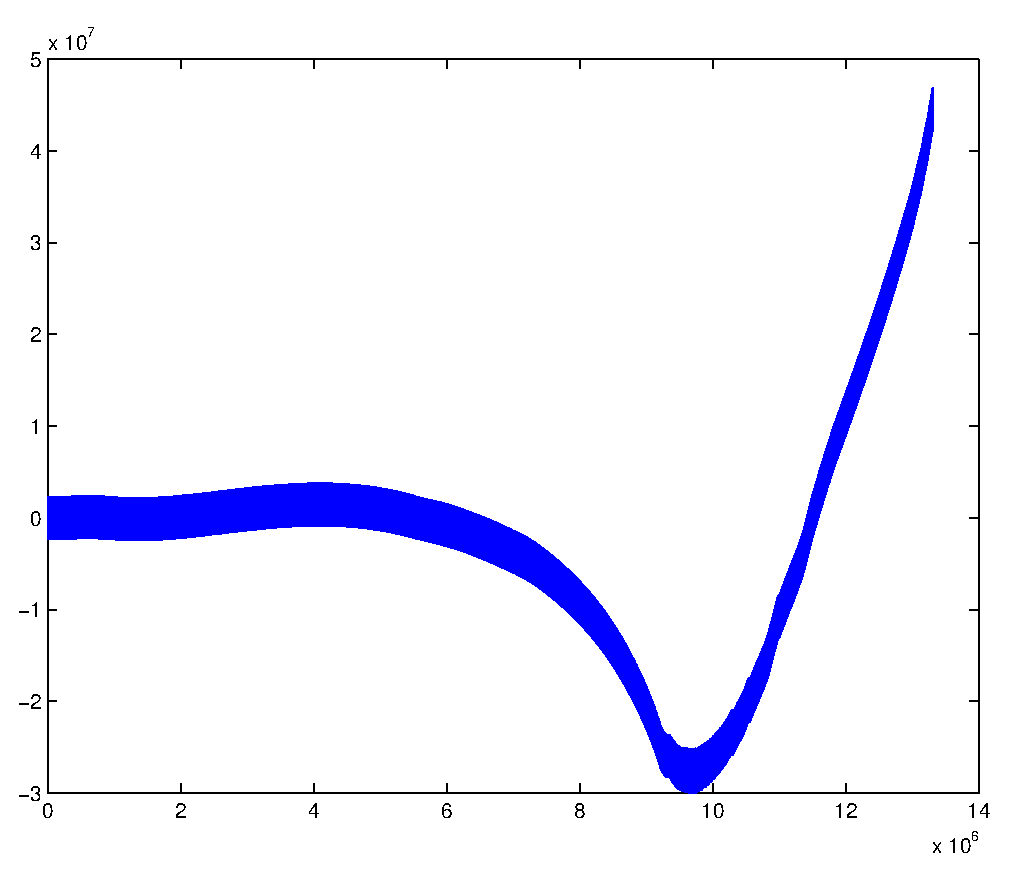
\includegraphics[width=12cm]{pics/teilch_in_em_welle_e.eps}\\
 \caption{Electron in EM Wave, E component}\label{fig_part_in_em_wave_e}
\end{figure}

\begin{figure}
  % Requires \usepackage{graphicx}
  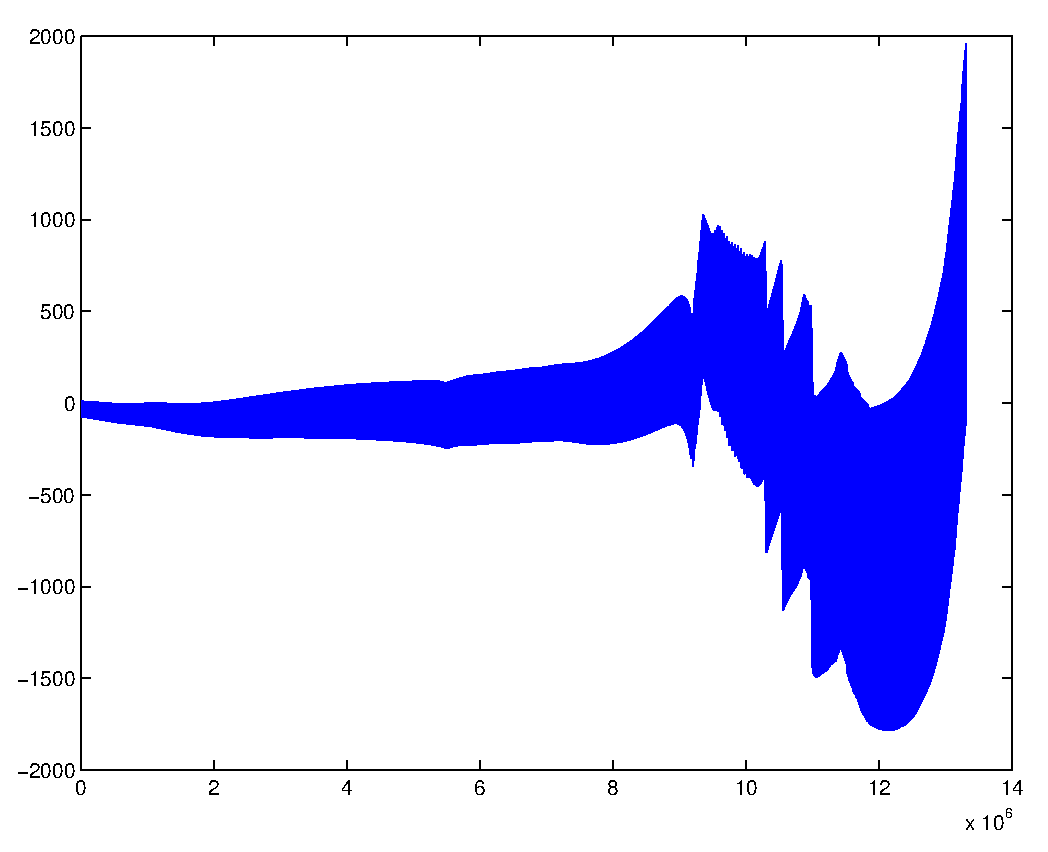
\includegraphics[width=12cm]{pics/teilch_in_em_welle_k.eps}\\
 \caption{Electron in EM Wave, k component}\label{fig_part_in_em_wave_k}
\end{figure}
\end{center}

which can be solved. Figures \ref{fig_part_in_em_wave_e} and \ref{fig_part_in_em_wave_k} show the numerical result of the velocity for the first 8.5 seconds. Equations \ref{firsttosolve} and \ref{secondtosolve} were used. The electron was initially at rest.

\subsection{Analytical solution of the simplified case}
From \ref{secondtosolve}:

\begin{eqnarray}
% \nonumber to remove numbering (before each equation)
\frac{m }{q E_0} \dot{v}_e e^{-i(\mathbf{k \cdot r}-\omega t)}&=&   1- \left( \frac{v_k k}{c} \right)  \\
\Rightarrow \left( \frac{v_k k}{c} \right)&=&   1- \frac{m}{q E_0} \dot{v}_e e^{-i(\mathbf{k \cdot r}-\omega t)}   \\
\Rightarrow v_k &=&   \frac{c}{k}- \frac{m c}{q E_0 k} \dot{v}_e e^{-i(\mathbf{k \cdot r}-\omega t)} \\
\Rightarrow \dot{v}_k &=& - \frac{i \omega m c}{q E_0 k} \dot{v}_e e^{-i(\mathbf{k \cdot r}-\omega t)} - \frac{ m c}{q E_0 k} \ddot{v}_e e^{-i(\mathbf{k \cdot r}-\omega t)}
\end{eqnarray}

Substituting this into \ref{firsttosolve}, gives

\begin{eqnarray}
% \nonumber to remove numbering (before each equation)
  - \frac{i \omega m c}{q E_0 k} \dot{v}_e e^{-i(\mathbf{k \cdot r}-\omega t)} - \frac{ m c}{q E_0 k} \ddot{v}_e e^{-i(\mathbf{k \cdot r}-\omega t)} &=& \frac{q k}{c m}(v_e E_0) e^{i(\mathbf{k \cdot r}-\omega t)} \\
\Rightarrow   \frac{ m c}{q E_0 k} \ddot{v}_e + \frac{i \omega m c}{q E_0 k} \dot{v}_e + \frac{q k E_0}{c m}  v_e e^{2i(\mathbf{k \cdot r}-\omega t)}  &=& 0\\
\Rightarrow   \ddot{v}_e + i \omega  \dot{v}_e + \frac{q^2 k^2 E_0^2}{c^2 m^2}  v_e e^{2i(\mathbf{k \cdot r}-\omega t)}  &=& 0
\end{eqnarray}

Umgekehrt...

\begin{eqnarray}
% \nonumber to remove numbering (before each equation)
  \dot{v}_k &=& \frac{q k}{c m}(v_e E_0) e^{i(\mathbf{k \cdot r}-\omega t)} \\
 \Rightarrow v_e &=& \frac{c m}{q k E_0} e^{-i(\mathbf{k \cdot r}-\omega t)}\dot{v}_k     \\
\Rightarrow \dot{v}_e &=& \frac{c m}{q k E_0} e^{-i(\mathbf{k \cdot r}-\omega t)}\ddot{v}_k   -  \frac{i \omega c m}{q k E_0} e^{-i(\mathbf{k \cdot r}-\omega t)}\dot{v}_k
\end{eqnarray}

Substituting :

\begin{eqnarray}
% \nonumber to remove numbering (before each equation)
\frac{c m}{q k E_0} \ddot{v}_k   -  \frac{i \omega c m}{q k E_0} \dot{v}_k &=& \frac{q }{m} E_0 \left( 1- \left( \frac{v_k k}{c} \right )\right) e^{2i(\mathbf{k \cdot r}-\omega t)}\\
\Rightarrow   \ddot{v}_k   -  i \omega \dot{v}_k + \frac{ E_0^2  q^2 k^2}{c^2 m^2} v_k  e^{2i(\mathbf{k \cdot r}-\omega t)} &=& \frac{q^2 E_0^2 k}{m^2 c}  e^{2i(\mathbf{k \cdot r}-\omega t)}
\end{eqnarray}

L�sung der ersten Gl. mit der Wronski Determinante...oder auch nicht,

\part{Magnetohydrodynamic effects}
\chapter{MHD basics}
\section{Basic equations}
\subsection{Force Density}
\paragraph*{}
The force on a particle is

\begin{equation}\label{force_on_particle}
    F=q\mathbf{E}+q\mathbf{v}\times \mathbf{B}=q\mathbf{E}+\mathbf{I}\times \mathbf{B}
\end{equation}

where \textbf{I} is the current. Dividing by the volume gives the force density

\begin{equation}\label{force_on_particle}
    f=\rho_e \mathbf{E}+\mathbf{j}\times \mathbf{B}
\end{equation}

$\rho_e$ is the charge density, \textbf{j} the current density. The magnetic term is dominant, so often the first term is neglected. If the conductivity is taken to approach infinity, no electric fields can sustain, so the first term is zero.

\subsection{The energy equation}
\paragraph*{}
Ohms law

\begin{equation}\label{ohm}
    \mathbf{j}=\sigma(\mathbf{E}+\mathbf{v} \times \mathbf{B})
\end{equation}

dotted on the left by the current density

\begin{equation}
    j^2=\sigma(\mathbf{j} \cdot \mathbf{E}+\mathbf{j} \cdot \mathbf{v} \times \mathbf{B})
\end{equation}

Using one of the Maxwell equations

\begin{equation}
    \frac{1}{\mu_0}\nabla \times \mathbf{B}=\mathbf{j}+\varepsilon_0 \frac{\partial \mathbf{E}}{\partial t} \label{maxwell_freespace4}
\end{equation}

gives

\begin{equation}\label{ohm}
    j^2=\sigma\left( \left( \frac{1}{\mu_0}\nabla \times \mathbf{B} \right) \cdot \mathbf{E}+\mathbf{j} \cdot \mathbf{v} \times \mathbf{B} \right)
\end{equation}

when the displacement current is ignored. Using further

\begin{equation}
    \nabla \cdot (\mathbf{E} \times \mathbf{B}) = \mathbf{B} \cdot (\nabla \times \mathbf{E}) - \mathbf{E} \cdot (\nabla \times \mathbf{B})
\end{equation}

and

\begin{equation}
    \nabla \times \mathbf{E}= -\frac{\partial \mathbf{B}}{\partial t} \label{maxwell_freespace3}
\end{equation}

we get

\begin{equation}
    \frac{j^2}{\sigma} +\frac{1}{\mu_0}\nabla \cdot (\mathbf{E} \times \mathbf{B})=  -\frac{1}{\mu_0}\mathbf{B} \cdot \frac{\partial \mathbf{B}}{\partial t} +\mathbf{j} \cdot \left( \mathbf{v} \times \mathbf{B} \right)
\end{equation}

or

\begin{equation}\label{ohm}
    \frac{j^2}{\sigma} +\nabla \cdot \mathbf{S}=  -\frac{1}{\mu_0} \frac{\partial \mathbf{B}^2}{\partial t} +\mathbf{j} \cdot \left( \mathbf{v} \times \mathbf{B} \right)
\end{equation}

when introducing the Poynting vector

\begin{equation} \label{poynting}\
\mathbf{S}=\mathbf{E} \times \mathbf{H}^* \nonumber
\end{equation}

In different form:

\begin{equation}\label{ohm}
    -\frac{1}{\mu_0} \frac{\partial \mathbf{B}^2}{\partial t}= \frac{j^2}{\sigma} +\nabla \cdot \mathbf{S}+\mathbf{v} \cdot \left( \mathbf{j} \times \mathbf{B} \right)
\end{equation}

The variation of magnetic field energy per time is equal to the negative of the sum of the joule heating, the Poynting flux and the work done to the system by the force density.


\subsection{System of equations}

\begin{eqnarray}
\nabla \cdot \mathbf{E}&=& \frac{\rho_e}{\varepsilon_0} \label{maxwell_freespace1}\\
\nabla \cdot \mathbf{B}&=& 0 \label{maxwell_freespace2}\\
\nabla \times \mathbf{E}&=& -\frac{\partial \mathbf{B}}{\partial t} \label{maxwell_freespace3}\\
\frac{1}{\mu_0}\nabla \times \mathbf{B}&=&\mathbf{j}+\varepsilon_0 \frac{\partial \mathbf{E}}{\partial t} \label{maxwell_freespace4}\\
\mathbf{j}&=&\sigma(\mathbf{E}+\mathbf{v} \times \mathbf{B})\label{ohm2}\\
P &=& P(\rho,T) \label{zustandsgl_allg} \\
\frac{d}{dt}\left( \frac{p}{\rho^\gamma } \right)&=&0 \label{thermodyn}\\
\frac{\partial \rho}{\partial t} &=& -\nabla \cdot (\rho \mathbf{v}) \label{continouity}\\
\rho \frac{\partial \mathbf{v}}{\partial t} + \rho (\mathbf{v} \cdot \nabla)\mathbf{v} &=& -\nabla P + \rho_e \mathbf{E}+\mathbf{j}\times \mathbf{B} + \rho \mathbf{g} + \rho \nu \nabla^2 \mathbf{v}\label{equation_of_motion}
\end{eqnarray}

That are 17 equations with 20 unknown parameters: $\mathbf{B}, \mathbf{E}, \mathbf{j}, \mathbf{v}, \mathbf{g}, \sigma, \rho, \rho_e,\nu$ and $T$.\\

An equivalent representation of the continuity eq. is

\begin{equation}\label{conti2}
    \frac{\partial n}{\partial t} = -\nabla \cdot (n \mathbf{v})
\end{equation}

\subsection{Basic equation according to \cite{baumjohann1}}
\subsubsection{Momentum equation}
An other version of the momentum equation can be derived by dividing (\ref{equation_of_motion}) by the mass of a particle.

\begin{equation}
    n \frac{\partial \mathbf{v}}{\partial t} + n (\mathbf{v} \cdot \nabla)\mathbf{v} = -\frac{1}{m}\nabla P + \frac{e n}{m} \mathbf{E}+\frac{1}{m}\mathbf{j}\times \mathbf{B} + n \mathbf{g} + n \nu \nabla^2 \mathbf{v}
\end{equation}

Then we can modify the first two terms and draw n into the differential.

\begin{eqnarray}
n \frac{\partial \mathbf{v}}{\partial t} + n (\mathbf{v} \cdot \nabla)\mathbf{v} &=& \frac{\partial n \mathbf{v}}{\partial t}-\mathbf{v} \frac{\partial n}{\partial t}+ n (\mathbf{v} \cdot \nabla)\mathbf{v}\\
&=& \frac{\partial n \mathbf{v}}{\partial t}+\mathbf{v} \nabla \cdot (n \mathbf{v})+ n (\mathbf{v} \cdot \nabla)\mathbf{v}\label{used_conti_eq}\\
&=& \frac{\partial n \mathbf{v}}{\partial t}+\mathbf{v }\nabla \cdot (n \mathbf{v})+ n \nabla \cdot (\mathbf{v}  \mathbf{v})-n\mathbf{v}(\nabla \cdot \mathbf{v})\\
&=& \frac{\partial n \mathbf{v}}{\partial t}+\mathbf{v }\mathbf{v}\nabla n\ +n\mathbf{v }(\nabla \cdot  \mathbf{v})+ n \nabla \cdot (\mathbf{v}  \mathbf{v})-n\mathbf{v}(\nabla \cdot \mathbf{v})\\
&=& \frac{\partial n \mathbf{v}}{\partial t}+\mathbf{v }\mathbf{v}\nabla n\ + n \nabla \cdot (\mathbf{v}  \mathbf{v})\\
&=& \frac{\partial n \mathbf{v}}{\partial t}+ \nabla \cdot (n \mathbf{v}  \mathbf{v})
\end{eqnarray}
To get (\ref{used_conti_eq}), I used the continuity equation. So the momentum equation becomes
\begin{equation}
     \frac{\partial n \mathbf{v}}{\partial t}+ \nabla \cdot (n \mathbf{v}  \mathbf{v}) = -\frac{1}{m}\nabla P + \frac{e n}{m} \mathbf{E}+\frac{1}{m}\mathbf{j}\times \mathbf{B} + n \mathbf{g} + n \nu \nabla^2 \mathbf{v}
\end{equation}

This equation can be directly derived from the Vlasov equation by taking the second moment. When employing the pressure tensor to model an anisotropic pressure, it becomes

\begin{equation}\label{momentum_equation}
     \frac{\partial n \mathbf{v}}{\partial t}+ \nabla \cdot (n \mathbf{v}  \mathbf{v}) = -\frac{1}{m}\nabla \cdot \mathbf{P} + \frac{e n}{m} \mathbf{E}+\frac{1}{m}\mathbf{j}\times \mathbf{B} + n \mathbf{g} + n \nu \nabla^2 \mathbf{v}
\end{equation}

When using the equation with the pressure tensor, another equation is needed, namely the energy equation. It can be derived by taking the second moment of the Vlasov equation.

\subsubsection{Energy equation}

\begin{equation}\label{energy_equ}
    \frac{3}{2}nk\left( \frac{\partial T}{\partial t} + \mathbf{v} \cdot \nabla T \right) + P \nabla \cdot \mathbf{v}=-\nabla \cdot \mathbf{q}- (\mathbf{P}'\cdot \nabla) \cdot \mathbf{v}
\end{equation}

\textbf{q} is the heat flux vector and \textbf{P}' is the stress part of the pressure tensor. The heat flux vector is then a new quantity, a product of the third moment. So another equation would be required, or the system can be truncated at this point. This can be done by assuming the existence of an equation of state, such that the energy equation is not required. The form of the equation of state manly depends on the pressure tensor. If the pressure is isotropic there is only one equation of state needed. The resulting system of equations is as in the original system (\ref{maxwell_freespace1})-(\ref{equation_of_motion}).\\

In the anisotropic case, the pressure tensor is the sum of a parallel and a perpendicular component.

\begin{equation}\label{anisotropic_pressure_tensor}
    \mathbf{P}=P_\bot \mathbf{I}+\left( P_\| - P_\bot \right)\frac{\mathbf{BB}}{B^2}
\end{equation}

In a coordinate system that is aligned such that the B field is along the z axis, it has the form

\begin{equation}\label{anisotropic_pressure_tensor_B_along_z}
    \mathbf{P}=\left( %
\begin{array}{ccc}
  P_\bot& 0 & 0 \\
  0 & P_\bot & 0 \\
  0 & 0 & P_\| \\
\end{array}%
\right)
\end{equation}


Using the concept of kinetic temperature, one can use the perpendicular and parallel temperature to derive two equations of state.

\begin{eqnarray}
  P_\bot &=& nkT_\bot \\
P_\| &=& nkT_\|
\end{eqnarray}

Since the degrees of freedom are different for the parallel and the perpendicular movement, there are 2 adiabatic equations necessary.

\begin{eqnarray}
   \frac{P_\bot}{\rho^2 } &=& const\\
\frac{P_\|}{\rho^3 } &=& const
\end{eqnarray}

or

\begin{eqnarray}
   \frac{P_\bot}{n^2 } &=& const\\
\frac{P_\|}{n^3 } &=& const
\end{eqnarray}

\subsubsection{Generalized Ohm's law}
An other equation for the current density can be found by using equation (\ref{momentum_equation}). For electrons and ions this is

\begin{eqnarray}
  \frac{\partial n_e \mathbf{v_e}}{\partial t}+ \nabla \cdot (n_e \mathbf{v_e}  \mathbf{v_e}) &=& -\frac{1}{m_e}\nabla \cdot \mathbf{P_e} - \frac{e n_e}{m_e} (\mathbf{E}+\mathbf{v_e}\times \mathbf{B}) + n_e \mathbf{g} + n_e \nu \nabla^2 \mathbf{v_e} \\
  \frac{\partial n_i \mathbf{v_i}}{\partial t}+ \nabla \cdot (n_i \mathbf{v_i}  \mathbf{v_i}) &=& -\frac{1}{m_i}\nabla \cdot \mathbf{P_i} + \frac{e n_i}{m_i} (\mathbf{E}+\mathbf{v_i}\times \mathbf{B}) + n_i \mathbf{g} + n_i \nu \nabla^2 \mathbf{v_i}
\end{eqnarray}

The isotropic pressure was used. We neglect the gravitational force, so

\begin{eqnarray}
  \frac{\partial n_e \mathbf{v_e}}{\partial t}+ \nabla \cdot (n_e \mathbf{v_e}  \mathbf{v_e}) &=& -\frac{1}{m_e}\nabla \cdot \mathbf{P_e} - \frac{e n_e}{m_e} (\mathbf{E}+\mathbf{v_e}\times \mathbf{B}) + n_e \nu \nabla^2 \mathbf{v_e} \\
  \frac{\partial n_i \mathbf{v_i}}{\partial t}+ \nabla \cdot (n_i \mathbf{v_i}  \mathbf{v_i}) &=& -\frac{1}{m_i}\nabla \cdot \mathbf{P_i} + \frac{e n_i}{m_i} (\mathbf{E}+\mathbf{v_i}\times \mathbf{B})  + n_i \nu \nabla^2 \mathbf{v_i}
\end{eqnarray}

When the current densities are small, we can neglect the terms that are quadratic in v.

\begin{eqnarray}
  \frac{\partial n_e \mathbf{v_e}}{\partial t} &=& -\frac{1}{m_e}\nabla \cdot \mathbf{P_e} - \frac{e n_e}{m_e} (\mathbf{E}+\mathbf{v_e}\times \mathbf{B}) + n_e \nu \nabla^2 \mathbf{v_e} \\
  \frac{\partial n_i \mathbf{v_i}}{\partial t}   &=& -\frac{1}{m_i}\nabla \cdot \mathbf{P_i} + \frac{e n_i}{m_i} (\mathbf{E}+\mathbf{v_i}\times \mathbf{B})  + n_i \nu \nabla^2 \mathbf{v_i}
\end{eqnarray}

Multiplying the ion equation by $m_e$

\begin{eqnarray}
  \frac{\partial n_e \mathbf{v_e}}{\partial t} &=& -\frac{1}{m_e}\nabla \cdot \mathbf{P_e} - \frac{e n_e}{m_e} (\mathbf{E}+\mathbf{v_e}\times \mathbf{B}) + n_e \nu \nabla^2 \mathbf{v_e} \\
  m_e \frac{\partial n_i \mathbf{v_i}}{\partial t}   &=& -\frac{m_e}{m_i}\nabla \cdot \mathbf{P_i} + \frac{e n_i m_e}{m_i} (\mathbf{E}+\mathbf{v_i}\times \mathbf{B})  + m_e n_i \nu \nabla^2 \mathbf{v_i}
\end{eqnarray}

A terms with the factor $\frac{m_e}{m_i}$ are very small and can be neglected.

\begin{eqnarray}
  \frac{\partial n_e \mathbf{v_e}}{\partial t} &=& -\frac{1}{m_e}\nabla \cdot \mathbf{P_e} - \frac{e n_e}{m_e} (\mathbf{E}+\mathbf{v_e}\times \mathbf{B}) + n_e \nu \nabla^2 \mathbf{v_e} \\
  m_e \frac{\partial n_i \mathbf{v_i}}{\partial t}   &=&   m_e n_i \nu \nabla^2 \mathbf{v_i}
\end{eqnarray}

Now I substract the equations

\begin{eqnarray}
  m_e \frac{\partial n_i \mathbf{v_i}}{\partial t}  -  \frac{\partial n_e \mathbf{v_e}}{\partial t} &=&   m_e n_i \nu \nabla^2 \mathbf{v_i} +\frac{1}{m_e}\nabla \cdot \mathbf{P_e} + \frac{e n_e}{m_e} (\mathbf{E}+\mathbf{v_e}\times \mathbf{B}) - n_e \nu \nabla^2 \mathbf{v_e} \\
\end{eqnarray}

\subsubsection{Alternate set of equations}

\begin{eqnarray}
\nabla \cdot \mathbf{B}&=& 0 \label{maxwell_freespace_baum}\\
\nabla \times \mathbf{E}&=& -\frac{\partial \mathbf{B}}{\partial t} \label{maxwell_freespace_baum}\\
\frac{1}{\mu_0}\nabla \times \mathbf{B}&=&\mathbf{j}+\varepsilon_0 \frac{\partial \mathbf{E}}{\partial t} \label{maxwell_freespace_baum}\\
\mathbf{E}+\mathbf{v} \times \mathbf{B} &=&  \eta + \frac{1}{ne}\mathbf{j}\times \mathbf{B}- \frac{1}{ne} \nabla \cdot \mathbf{P}_e +  \frac{m_e}{ne^2} \frac{\partial \mathbf{j}}{\partial t} \label{ohm_baum}\\
\frac{\partial n}{\partial t} +\nabla \cdot (n \mathbf{v}) &=&0\label{continouity_baum}\\
  \frac{\partial n \mathbf{v}}{\partial t}+ \nabla \cdot (n \mathbf{v}  \mathbf{v}) &=& -\frac{1}{m}\nabla \cdot \mathbf{P} + \frac{e n}{m} \mathbf{E}+\frac{1}{m}\mathbf{j}\times \mathbf{B} + n \mathbf{g} + n \nu \nabla^2 \mathbf{v}\label{equation_of_motion_baum}
\end{eqnarray}

\subsection{Basic equation according to \cite{landau_lifschitz_8}}

\subsubsection{Alternate set of equations}

\begin{eqnarray}
\nabla \cdot \mathbf{H}&=& 0 \label{maxwell_freespace_ll}\\
 \frac{\partial \mathbf{H}}{\partial t} &=& \nabla \times (\mathbf{v} \times \mathbf{H})+\frac{c^2}{4 \pi \sigma} \nabla^2 \mathbf{H}\label{maxwell_freespace_ll}\\
\frac{\partial \rho}{\partial t} +\nabla \cdot (\rho \mathbf{v}) &=& 0\label{continouity_ll}\\
  \frac{\partial  \mathbf{v}}{\partial t}+ ( \mathbf{v} \cdot \nabla ) \mathbf{v}   &=& -\frac{\nabla P}{\rho }  - \frac{1}{4 \pi \rho } (\mathbf{H} \times (\nabla \times \mathbf{H})) +\frac{\eta }{\rho }\nabla^2 \mathbf{v} + \frac{1}{\rho}\left( \zeta +\frac{\eta }{3}\right) \nabla(\nabla \cdot \mathbf{v})\label{equation_of_motion_ll}\\
P &=& P(\rho,T) \label{zustandsgl_ll}\\
\rho T \left( \frac{\partial s}{\partial t}+\mathbf{v} \nabla s \right) &=& \sigma^{'}_{ik} \frac{\partial v_i}{\partial x_k}+ \nabla \cdot (\chi \nabla T) + \frac{c^2}{16 \pi^2 \sigma} (\nabla \times \mathbf{H})^2
\end{eqnarray}

For detailed description see \cite{landau_lifschitz_8}.
\subsection{Possible simplifications}
Often the gravitational field can be neglected. Also, in a collision-less plasma, the viscosity term van be neglected. Also, the ideal gas equation can be used Then we have

\begin{eqnarray}
\nabla \cdot \mathbf{E}&=& \frac{\rho_e}{\varepsilon_0} \label{maxwell_freespace1_simpli1}\\
\nabla \cdot \mathbf{B}&=& 0 \label{maxwell_freespace2_simpli1}\\
\nabla \times \mathbf{E}&=& -\frac{\partial \mathbf{B}}{\partial t} \label{maxwell_freespace3_simpli1}\\
\frac{1}{\mu_0}\nabla \times \mathbf{B}&=&\mathbf{j}+\varepsilon_0 \frac{\partial \mathbf{E}}{\partial t} \label{maxwell_freespace4_simpli1}\\
\mathbf{j}&=&\sigma(\mathbf{E}+\mathbf{v} \times \mathbf{B})\label{ohm2_simpli1}\\
P &=& nkT \label{zustandsgl_allg_simpli1} \\
\frac{d}{dt}\left( \frac{P}{\rho^\gamma } \right)&=&0 \label{thermodyn_simpli1}\\
\frac{\partial \rho}{\partial t} &=& -\nabla \cdot (\rho \mathbf{v}) \label{continouity_simpli1}\\
\rho \frac{\partial \mathbf{v}}{\partial t} + \rho (\mathbf{v} \cdot \nabla)\mathbf{v} &=& -\nabla P + \rho_e \mathbf{E}+\mathbf{j}\times \mathbf{B} \label{equation_of_motion_simpli1}
\end{eqnarray}

Then we have 17 equations with 18 unknown parameters: $\mathbf{B}, \mathbf{E}, \mathbf{j}, \mathbf{v}, \sigma, \rho, \rho_e$ and $T$.\\

The plasma conductivity has the equation

\begin{equation}\label{plasma_conductivity}
    \sigma=\frac{ne^2}{m_e \nu_c}
\end{equation}

$\nu_c$ is the collision frequency\cite{baumjohann1}. If there are no collisions, it is 0 and the conductivity is infinite.\\

If we set the conductivity to quasi infinity, there can build up no electric field. Also, ohm's law gets a different form because $\frac{\mathbf{j}}{\sigma}=0$

\begin{eqnarray}
\nabla \cdot \mathbf{E}&=& \frac{\rho_e}{\varepsilon_0} \label{maxwell_freespace1_simpli2}\\
\nabla \cdot \mathbf{B}&=& 0 \label{maxwell_freespace2_simpli2}\\
\nabla \times \mathbf{E}&=& -\frac{\partial \mathbf{B}}{\partial t} \label{maxwell_freespace3_simpli2}\\
\frac{1}{\mu_0}\nabla \times \mathbf{B}&=&\mathbf{j}+\varepsilon_0 \frac{\partial \mathbf{E}}{\partial t} \label{maxwell_freespace_simpli2}\\
\mathbf{E}+\mathbf{v} \times \mathbf{B}&=&0 \label{ohm2_simpli2}\\
P &=& nkT \label{zustandsgl_allg_simpli2} \\
\frac{d}{dt}\left( \frac{P}{\rho^\gamma } \right)&=&0 \label{thermodyn_simpli2}\\
\frac{\partial \rho}{\partial t} &=& -\nabla \cdot (\rho \mathbf{v}) \label{continouity_simpli2}\\
\rho \frac{\partial \mathbf{v}}{\partial t} + \rho (\mathbf{v} \cdot \nabla)\mathbf{v} &=& -\nabla P +\mathbf{j}\times \mathbf{B} \label{equation_of_motion_simpli2}
\end{eqnarray}

We have 17 equations with 17 unknown parameters, so this would be a useful system. I call it EMHD equations: $\mathbf{B}, \mathbf{E}, \mathbf{j}, \mathbf{v}, \rho, \rho_e$ and $T$.\\


When we regard only waves with low frequencies, we can neglect the displacement current, because the derivative of the electric field is small.

\begin{eqnarray}
\nabla \cdot \mathbf{E}&=& \frac{\rho_e}{\varepsilon_0} \label{maxwell_freespace1_simpli3}\\
\nabla \cdot \mathbf{B}&=& 0 \label{maxwell_freespace2_simpli3}\\
\nabla \times \mathbf{E}&=& -\frac{\partial \mathbf{B}}{\partial t} \label{maxwell_freespace3_simpli3}\\
\frac{1}{\mu_0}\nabla \times \mathbf{B}&=&\mathbf{j} \label{maxwell_freespace_simpli3}\\
\mathbf{E}+\mathbf{v} \times \mathbf{B}&=&0 \label{ohm2_simpli3}\\
P &=& nkT \label{zustandsgl_allg_simpli3} \\
\frac{d}{dt}\left( \frac{P}{\rho^\gamma } \right)&=&0 \label{thermodyn_simpli3}\\
\frac{\partial \rho}{\partial t} &=& -\nabla \cdot (\rho \mathbf{v}) \label{continouity_simpli3}\\
\rho \frac{\partial \mathbf{v}}{\partial t} + \rho (\mathbf{v} \cdot \nabla)\mathbf{v} &=& -\nabla P +\mathbf{j}\times \mathbf{B} \label{equation_of_motion_simpli3}
\end{eqnarray}

Alternative form der Konti Gl.:

\begin{equation}\label{other_conti}
    \frac{D \rho}{Dt}+\rho \nabla \cdot \mathbf{v}=0
\end{equation}

If the system is time dependent, the solenoidity is a necessary result of Faraday's equation, so

\begin{eqnarray}
\nabla \cdot \mathbf{E}&=& \frac{\rho_e}{\varepsilon_0} \label{maxwell_freespace1_simpli4}\\
\nabla \times \mathbf{E}&=& -\frac{\partial \mathbf{B}}{\partial t} \label{maxwell_freespace3_simpli4}\\
\frac{1}{\mu_0}\nabla \times \mathbf{B}&=&\mathbf{j} \label{maxwell_freespace_simpli4}\\
\mathbf{E}+\mathbf{v} \times \mathbf{B}&=&0 \label{ohm2_simpli4}\\
P &=& nkT \label{zustandsgl_allg_simpli3} \\
\frac{d}{dt}\left( \frac{P}{\rho^\gamma } \right)&=&0 \label{thermodyn_simpli4}\\
\frac{\partial \rho}{\partial t} &=& -\nabla \cdot (\rho \mathbf{v}) \label{continouity_simpli4}\\
\rho \frac{\partial \mathbf{v}}{\partial t} + \rho (\mathbf{v} \cdot \nabla)\mathbf{v} &=& -\nabla P +\mathbf{j}\times \mathbf{B} \label{equation_of_motion_simpli4}
\end{eqnarray}

is enough: We have 16 equations with 17 unknown parameters.\\

If we know the temperature (isothermal case), we can remove either the gas equation or the adiabatic equation:

\begin{eqnarray}
\nabla \cdot \mathbf{E}&=& \frac{\rho_e}{\varepsilon_0} \label{maxwell_freespace1_simpli5}\\
\nabla \times \mathbf{E}&=& -\frac{\partial \mathbf{B}}{\partial t} \label{maxwell_freespace3_simpli5}\\
\frac{1}{\mu_0}\nabla \times \mathbf{B}&=&\mathbf{j} \label{maxwell_freespace_simpli5}\\
\mathbf{E}+\mathbf{v} \times \mathbf{B}&=&0 \label{ohm2_simpli5}\\
\frac{d}{dt}\left( \frac{P}{\rho^\gamma } \right)&=&0 \label{thermodyn_simpli4}\\
\frac{\partial \rho}{\partial t} &=& -\nabla \cdot (\rho \mathbf{v}) \label{continouity_simpli4}\\
\rho \frac{\partial \mathbf{v}}{\partial t} + \rho (\mathbf{v} \cdot \nabla)\mathbf{v} &=& -\nabla P +\mathbf{j}\times \mathbf{B} \label{equation_of_motion_simpli4}
\end{eqnarray}

15 equations with 16 unknown parameters.\\

The equation of motion and Ampere's law can be combined:

\begin{eqnarray}
    \rho \frac{\partial \mathbf{v}}{\partial t} + \rho (\mathbf{v} \cdot \nabla)\mathbf{v} &=& -\nabla P +\frac{1}{\mu_0}\nabla \times \mathbf{B}\times \mathbf{B}\\
&=& -\nabla P -\frac{1}{\mu_0} \mathbf{B} \times \nabla \times \mathbf{B}
\end{eqnarray}

And Ohm's, Faraday's and Ampere's law can be combined. too.

\begin{eqnarray}
\mathbf{j}&=&\sigma(\mathbf{E}+\mathbf{v} \times \mathbf{B})\\
\rightarrow \nabla \times \mathbf{B}&=& \mu_0 \sigma(\mathbf{E}+\mathbf{v} \times \mathbf{B})
\end{eqnarray}

Taking the rotation of the equation results in

\begin{eqnarray}
-\nabla^2 \mathbf{B}&=& \mu_0 \sigma( \nabla \times \mathbf{E}+ \nabla \times (\mathbf{v} \times \mathbf{B}))\\
-\nabla^2 \mathbf{B}&=& \mu_0 \sigma( -\frac{\partial \mathbf{B}}{\partial t} + \nabla \times (\mathbf{v} \times \mathbf{B}))\\
\frac{\partial \mathbf{B}}{\partial t} &=& \frac{1}{\mu_0 \sigma} \nabla^2 \mathbf{B}  + \nabla \times (\mathbf{v} \times \mathbf{B}))
\end{eqnarray}

So the new system of equations is

\begin{eqnarray}
 \rho \frac{\partial \mathbf{v}}{\partial t} + \rho (\mathbf{v} \cdot \nabla)\mathbf{v}&=&  -\nabla P -\frac{1}{\mu_0} \mathbf{B} \times (\nabla \times \mathbf{B})\\
\frac{D \rho}{Dt}+\rho \nabla \cdot \mathbf{v}&=&0\\
\nabla \cdot \mathbf{B}&=& 0\\
 \frac{d}{dt}\left( \frac{P}{\rho^\gamma } \right)&=&0\\
\frac{\partial \mathbf{B}}{\partial t} &=& \frac{1}{\mu_0 \sigma} \nabla^2 \mathbf{B}  + \nabla \times (\mathbf{v} \times \mathbf{B}))
\end{eqnarray}

So these are 9 equations with 9 parameters, if the conductivity is taken as a parameter.  $\mathbf{B}, \mathbf{v}, \sigma, \rho, P$ .\\

\subsubsection{Further simplification of Newton II}

Using the identity

\begin{equation}
    \nabla (\mathbf{A}\cdot \mathbf{B})=(\mathbf{A} \cdot \nabla)  \mathbf{B}+(\mathbf{B} \cdot \nabla)  \mathbf{A}+\mathbf{A} \times (\nabla \times \mathbf{B})+\mathbf{B} \times (\nabla \times \mathbf{A})
\end{equation}

for any vector fields \textbf{A} and \textbf{B}, we can write for our special case

\begin{eqnarray}
   \nabla (\mathbf{B}\cdot \mathbf{B})&=&(\mathbf{B} \cdot \nabla)  \mathbf{B}+(\mathbf{B} \cdot \nabla)  \mathbf{B}+\mathbf{B} \times (\nabla \times \mathbf{B})+\mathbf{B} \times (\nabla \times \mathbf{B}) \\
  \nabla B^2&=&2(\mathbf{B} \cdot \nabla)  \mathbf{B}+2\mathbf{B} \times (\nabla \times \mathbf{B}) \\
\mathbf{B} \times (\nabla \times \mathbf{B} )&=& \nabla \frac{B^2}{2}-(\mathbf{B} \cdot \nabla)  \mathbf{B}
\end{eqnarray}

So the equation of motion becomes

\begin{eqnarray}
 \rho \frac{\partial \mathbf{v}}{\partial t} + \rho (\mathbf{v} \cdot \nabla)\mathbf{v}&=&  -\nabla P -\frac{1}{\mu_0} \mathbf{B} \times (\nabla \times \mathbf{B})\\
&=& -\frac{1}{\mu_0} \left( \nabla \frac{B^2}{2}-(\mathbf{B} \cdot \nabla)  \mathbf{B} \right)  -\nabla P\\
&=& \frac{1}{\mu_0} (\mathbf{B} \cdot \nabla)  \mathbf{B}  -\nabla \left( \frac{B^2}{2\mu_0} +P  \right)
\end{eqnarray}

In tensor notation

\begin{eqnarray}
 \rho \frac{\partial v_i}{\partial t} + \rho v_j \partial_j v_i &=& \frac{1}{\mu_0} B_j \partial_j  B_i  -\partial_i \left( \frac{B_l B_l}{2\mu_0} +P  \right)\\
\rho \frac{\partial v_i}{\partial t}  &=& - \partial_j \rho v_j  v_i + \partial_j \frac{1}{\mu_0} B_j  B_i  - \partial_j \delta_{i j} \left( \frac{B_l B_l}{2\mu_0} +P  \right)\\
 &=& - \partial_j \left( \rho v_j  v_i -  \frac{1}{\mu_0} B_j  B_i  +  \delta_{i j} \left( \frac{B_l B_l}{2\mu_0} +P  \right) \right)\\
&=& - \partial_j P_{ij}
\end{eqnarray}

where $P_{ij}$ is the Maxwellian stress tensor. This equation represents also the conservation of momentum.


\subsection{Validity of MHD}
Since the theory does not make any distinction between the components, it can only be used to model phenomena that have a characteristic timescale that is longer than the longest characteristic period of any component. This is normally the cyclotron frequency of the heaviest ion.\\

In our case, however, it seems that the time scale of the plasma frequency is longer. So I think the MHD equations can be used up to a frequency of a few 10 kHz.


\part{Kinetic effects}


\chapter{Basics of the kinetic plasma theory}
\section{Exact phase space}

A plasma consists of many particles of different kind, interacting with each other. Each particle is fully defined by its charge, mass, position vector $\mathbf{q}$ and momentum vector $\mathbf{p}$. When a different set of equations is used for each species, there are two possibilities how to represent the plasma system. The way, I will use, is a 6 dimensional phase space, where each particle is represented by a point. The other possibility is to use a 6N space, where N is the number of particles of this species. Then the momentary state of the system is represented by a single point. The whole procedure, I describe is derived in a more detailed way in \cite{baumjohann1}.

When using the 6 dimensional representation, the exact number density of a particle can be written as

\begin{equation}\label{exact_number_density_one_particle}
    f_{exact,i}(\mathbf{q,p},t)=\delta(\mathbf{q}-\mathbf{q}_i(t))\delta(\mathbf{p}-\mathbf{p}_i(t))
\end{equation}

So the whole exact number density is

\begin{equation}\label{exact_number_density}
f_{exact}(\mathbf{q,p},t)=\sum_i \delta(\mathbf{q}-\mathbf{q}_i(t))\delta(\mathbf{p}-\mathbf{p}_i(t))
\end{equation}

If the total number of particles is taken to be constant, we can say that a volume in the phase space, dV does not change its size during its evolvement in time, but merely changes its shape. So we can write

\begin{equation}\label{erhaltung_exact_number_density}
\frac{D}{Dt}f_{exact}(\mathbf{q,p},t)=\left( \frac{\partial}{\partial t} + \mathbf{v}\cdot \nabla_q+\frac{\partial \mathbf{p}}{\partial t}\cdot\nabla_p \right) f_{exact}(\mathbf{q,p},t)=0
\end{equation}

$\frac{D}{Dt}$ is the substantial derivative. $\frac{\partial \mathbf{p}}{\partial t}$ is the force, which is $q(\mathbf{E}+\mathbf{v}\times \mathbf{B})$ in our case, so

\begin{equation}\label{Klimontovich-Dupree}
\left( \frac{\partial}{\partial t} + \mathbf{v}\cdot \nabla_q+q(\mathbf{E}_m+\mathbf{v}\times \mathbf{B}_m)\cdot\nabla_p \right) f_{exact}(\mathbf{q,p},t)=0
\end{equation}

This important equation is called the \emph{Klimontovich-Dupree equation}. Subscript m indicates that the microscopic fields are meant.

\section{The average Distribution function}
We define the averaged phase space density.

\begin{equation}\label{f_av}
f=\langle f_{exact}(\mathbf{q,p},t) \rangle
\end{equation}

So the exact phase state density consists of two parts, the averaged phase space density and a fluctuation term.

\begin{equation}\label{f_exact}
f_{exact}=f+ \delta f_{exact}(\mathbf{q,p},t)
\end{equation}

$\langle \delta f_{exact}(\mathbf{q,p},t) \rangle =0$ must be true. Similar

\begin{eqnarray}
\mathbf{E}_m(\mathbf{q,p},t) &=& \mathbf{E}(\mathbf{q,p},t)+\delta \mathbf{E}(\mathbf{q,p},t) \\
\mathbf{B}_m (\mathbf{q,p},t)&=& \mathbf{B}(\mathbf{q,p},t)+\delta \mathbf{B}(\mathbf{q,p},t) \\
\langle \delta \mathbf{E}(\mathbf{q,p},t) \rangle &=& 0 \\
\langle \delta \mathbf{B}(\mathbf{q,p},t) \rangle &=& 0
\end{eqnarray}

Inserting these equations into (\ref{Klimontovich-Dupree}) yields the kinetic equation.

\begin{equation}\label{kinetic_equation}
\left( \frac{\partial}{\partial t} + \mathbf{v}\cdot \nabla_q+q(\mathbf{E}+\mathbf{v}\times \mathbf{B})\cdot\nabla_p \right) f(\mathbf{q,p},t)+ q(\mathbf{\delta E}+\mathbf{v}\times \mathbf{\delta B})\cdot\nabla_p \delta f(\mathbf{q,p},t)=0
\end{equation}

It describes the evolution of the coarse grained phase state density under influence of the averaged fields. The value of the distribution function f can be interpreted as the probability to find a particle in the volume d\textbf{q}d\textbf{p} of the phase space. The last term models the interaction between fields and particles. When collisions between particles are to be considered, there might be additional terms. Space plasma can be regarded as collision less most of the time, so I will neglect the collision term and even the EM interaction term in equation (\ref{kinetic_equation}). Then I get the simplest kinetic equation that can be used to describe plasma, the Vlasov equation.

\begin{equation}\label{vlasov1}
\left( \frac{\partial}{\partial t} + \mathbf{v}\cdot \nabla_q+q(\mathbf{E}+\mathbf{v}\times \mathbf{B})\cdot\nabla_p \right) f(\mathbf{q,p},t) =0
\end{equation}

This equation can also be written in a slightly different form, where index e describes the distribution function for the electrons, i for the ions.

\begin{eqnarray}
\left( \frac{\partial}{\partial t} + \mathbf{v_e}\cdot \nabla_q-\frac{e}{m_e}(\mathbf{E}+\mathbf{v_e}\times \mathbf{B})\cdot\nabla_v \right) f_e(\mathbf{q,v},t) &=& 0 \label{vlasov_e}\\
\left( \frac{\partial}{\partial t} + \mathbf{v_i}\cdot \nabla_q+\frac{Ze}{m_i}(\mathbf{E}+\mathbf{v_i}\times \mathbf{B})\cdot\nabla_v \right) f_i(\mathbf{q,v},t) &=& 0\label{vlasov_i}
\end{eqnarray}

These equations can be manipulated in a way to produce the equations of the two fluid theory, as shown in \cite{kippenhahn}, so two fluid theory is a subset of the kinetic theory.

\section{The Liouville theorem}
If collisions and interactions between particles and microscopic fields can be neglected, such that $\nabla \cdot \mathbf{v}=0$, as in case of Vlasov's equation, Liouville's theorem holds, which states that a phase space volume does not change, it marly can be deformed. This is a result of the conservation of particle numbers, so it holds exactly only for exact phase state density. In averaged phase space, it is only an approximation, although normally a good one.

A volume in phase space $dV$ moves under the action of the Lorenz force like an incompressible fluid. The reason for this behavior is that the divergency of the velocity is zero.

\section{The macroscopic observables}
To get macroscopic observables, which do not depend on the velocity distribution but are the result of it, one has to take the respective velocity moment of the distribution, that is, integrate over the velocity space to get rid of the velocity dependance.

\begin{equation}\label{velocity_moment_allgemein}
M_i(\mathbf{q},t)=\int \mathbf{v}^i f(\mathbf{q,v},t)d^3v
\end{equation}

$\mathbf{v}^i$ is the dyadic product of the velocity vector with itself, i times. The first four moments are the interesting ones. When we integrate the distribution function over the whole phase space we get the number of particles:

 \begin{equation}\label{particle number}
 N(\mathbf{q,v},t)=\int_V \int_v f(\mathbf{q,v},t)d^3v d^3q
 \end{equation}

 When You divide this n umber by the volume, You get the number density:

\begin{equation}
\label{velocity_moment_number_density}    n(\mathbf{q},t)=\int f(\mathbf{q,v},t)d^3v
\end{equation}

Then the bulk velocity,

\begin{equation}\label{velocity_moment_bulc_velocity}
\mathbf{v}_b(\mathbf{q},t)=\frac{1}{n}\int \mathbf{v} f(\mathbf{q,v},t)d^3v
\end{equation}

the pressure tensor, where we integrate over the velocity fluctuations

\begin{equation}\label{velocity_moment_pressure}
\mathbf{P}(\mathbf{q},t)=m\int (\mathbf{v}-\mathbf{v}_b)^2 f(\mathbf{q,v},t)d^3v
\end{equation}

and the heat tensor.

\begin{equation}\label{velocity_moment_heat_tensor}
\mathbf{Q}(\mathbf{q},t)=m\int (\mathbf{v}-\mathbf{v}_b)^3 f(\mathbf{q,v},t)d^3v
\end{equation}

the trace of the heat tensor corresponds to the heat flux vector.

\begin{equation}\label{heat_flux}
\mathbf{\phi}_H(\mathbf{q},t)=\frac{1}{2} m\int (\mathbf{v}-\mathbf{v}_b)\cdot(\mathbf{v}-\mathbf{v}_b)^2 f(\mathbf{q,v},t)d^3v
\end{equation}

the trace of the pressure tensor, which corresponds tho the isotropic part of the pressure, called thermal pressure, can be used to define to a scalar temperature of the plasma component, which is called kinetic temperature. \begin{equation}\label{kinetic_temperature}
T(\mathbf{q},t)=\frac{m}{2kn}\int (\mathbf{v}-\mathbf{v}_b) \cdot (\mathbf{v}-\mathbf{v}_b) f(\mathbf{q,v},t)d^3v \end{equation}

This temperature is not the same as the thermodynamic temperature which is defined only for a system in equilibrium. The kinetic temperature is a directed parameter. In an anisotropic plasma, it has different values for different directions, because the velocity distributions differ.

\section{Maxwell equations}
Taking into account the velocity distributions of the plasma, the Maxwell equations can be written accordingly:

\begin{eqnarray}
% \nonumber to remove numbering (before each equation)
  \nabla \cdot \mathbf{E} &=& \frac{1}{\epsilon_0}\sum_s q_s \int f_s(\mathbf{q,v},t)d^3v \\
\nabla \times \mathbf{H}- \epsilon_0 \frac{\partial \mathbf{E}}{\partial t}&=& \sum_s q_s \int \mathbf{v} f_s(\mathbf{q,v},t)d^3v \\
\nabla \times \mathbf{E} + \mu_0 \frac{ \partial \mathbf{H}}{\partial t} &=& 0 \\
\mu_0 \nabla \cdot \mathbf{H} &=& 0
\end{eqnarray}

where subscript s denotes the species of the particles.

\part{Plasma Waves}
\chapter{MHD waves}
\section{Linearized perturbation theory}
\subsection{Equations}
A linearized perturbation theory is used. The perturbed parameters consist of an unperturbed part with index 0 and a perturbed part with index 1. Hence:

\begin{eqnarray}
  \mathbf{B} &=& \mathbf{B}_0+\mathbf{B}_1 \\
 \mathbf{E} &=& \mathbf{E}_0+\mathbf{E}_1 \\
 \mathbf{j} &=& \mathbf{j}_0+\mathbf{j}_1 \\
 \mathbf{v} &=& \mathbf{v}_0+\mathbf{v}_1 \\
P &=& P_0+P_1 \\
\rho &=& \rho_0 + \rho_1
\end{eqnarray}

As basis for the system of equations we can take \ref{maxwell_freespace1} to \ref{equation_of_motion}, neglecting gravitation, viscosity and the displacement current. Conductivity approaches infinity, so there can exist no electric fielf.

\begin{eqnarray}
\nabla \cdot \mathbf{B}&=& 0 \\
\nabla \times \mathbf{E}&=& -\frac{\partial \mathbf{B}}{\partial t} \\
\frac{1}{\mu_0}\nabla \times \mathbf{B}&=&\mathbf{j}\\
\mathbf{E}&=&-\mathbf{v} \times \mathbf{B}\\
P &=& P(\rho,T)  \\
\frac{d}{dt}\left( \frac{p}{\rho^\gamma } \right)&=&0\\
\frac{\partial \rho}{\partial t} &=& -\nabla \cdot (\rho \mathbf{v}) \\
\rho \frac{\partial \mathbf{v}}{\partial t} + \rho (\mathbf{v} \cdot \nabla)\mathbf{v} &=& -\nabla P +\mathbf{j}\times \mathbf{B}
\end{eqnarray}

For the undisturbed parameters:

\begin{eqnarray}
\nabla \cdot \mathbf{B}_0&=& 0 \\
\nabla \times \mathbf{E}_0&=&0 \\
\frac{1}{\mu_0}\nabla \times \mathbf{B}_0&=&\mathbf{j}_0\\
\mathbf{E}_0&=&-\mathbf{v}_0 \times \mathbf{B}_0\\
P_0 &=& P_0(\rho,T)  \\
\frac{d}{dt}\left( \frac{p}{\rho^\gamma } \right)&=&0\\
\nabla \cdot (\rho_0 \mathbf{v}_0)&=&0 \\
 \rho_0 (\mathbf{v}_0 \cdot \nabla) \mathbf{v}_0 &=& -\nabla P_0 +\mathbf{j}_0 \times \mathbf{B}_0
\end{eqnarray}

The undisturbed magnetic field shall point only in x direction $B_0=B_{x,0}$ and $\mathbf{v}_0$ shall be zero.

\begin{eqnarray}
\frac{\partial B_0}{\partial x}&=& 0\label{einsicht1} \\
\frac{\partial }{\partial t} whatever_0&=&0\\
\mathbf{E}_0=\mathbf{0}\\
\mathbf{j}_0&=&\mathbf{0}\\
P_0 &=& P_0(\rho,T)  \\
\frac{d}{dt}\left( \frac{p}{\rho^\gamma } \right)&=&0\\
 \nabla P_0 &=&\mathbf{0}\label{einsicht6}
\end{eqnarray}

so

\begin{eqnarray}
\nabla \cdot (\mathbf{B}_0 + \mathbf{B}_1)&=& 0 \\
\nabla \times (\mathbf{E}_0 + \mathbf{E}_1)&=& -\frac{\partial }{\partial t} (\mathbf{B}_0 + \mathbf{B}_1)\\
\frac{1}{\mu_0}\nabla \times (\mathbf{B}_0 + \mathbf{B}_1)&=&(\mathbf{j}_0 + \mathbf{j}_1)\\
(\mathbf{E}_0 + \mathbf{E}_1)&=&-((\mathbf{v}_0 + \mathbf{v}_1) \times (\mathbf{B}_0 + \mathbf{B}_1))\\
(P_0+P_1) &=& (P_0+P_1)(\rho,T)  \\
\frac{d}{dt}\left( \frac{p_0+p_1}{(\rho_0+\rho_1)^\gamma } \right)&=&0\\
\frac{\partial (\rho_0+\rho_1)}{\partial t} &=& -\nabla \cdot ((\rho_0+\rho_1) (\mathbf{v}_0 + \mathbf{v}_1)) \\
(\rho_0+\rho_1) \frac{\partial (\mathbf{v}_0 + \mathbf{v}_1)}{\partial t} + (\rho_0+\rho_1) ((\mathbf{v}_0 + \mathbf{v}_1) \cdot \nabla)(\mathbf{v}_0 + \mathbf{v}_1) &=& -\nabla (P_0 + P_1) +(\mathbf{j}_0 + \mathbf{j}_1)\times(\mathbf{B}_0 + \mathbf{B}_1)
\end{eqnarray}

Using (\ref{einsicht1})-(\ref{einsicht6})

\begin{eqnarray}
\nabla \cdot \mathbf{B}_0 = \nabla \cdot \mathbf{B}_1&=& 0 \\
\nabla \times  \mathbf{E}_1&=& -\frac{\partial }{\partial t}  \mathbf{B}_1\\
\frac{1}{\mu_0}\nabla \times  \mathbf{B}_1&=&\mathbf{j}_1\\
\mathbf{E}_1&=&- \mathbf{v}_1 \times (\mathbf{B}_0 + \mathbf{B}_1)\\
(P_0+P_1) &=& (P_0+P_1)(\rho,T)  \\
\frac{d}{dt}\left( \frac{p_1}{\rho_1^\gamma } \right)&=&0\\
\frac{\partial \rho_1}{\partial t} &=& -\nabla \cdot ((\rho_0+\rho_1)   \mathbf{v}_1) \\
(\rho_0+\rho_1) \frac{\partial  \mathbf{v}_1}{\partial t} + ((\rho_0+\rho_1)  \mathbf{v}_1 \cdot \nabla) \mathbf{v}_1 &=& -\nabla P_1 + \mathbf{j}_1\times(\mathbf{B}_0 + \mathbf{B}_1)
\end{eqnarray}

If the perturbations are small, I can neglect all multiples of parameters with index 1.

\begin{eqnarray}
\nabla \cdot \mathbf{B}_0 = \nabla \cdot \mathbf{B}_1&=& 0 \\
\nabla \times  \mathbf{E}_1&=& -\frac{\partial }{\partial t}  \mathbf{B}_1\\
\frac{1}{\mu_0}\nabla \times  \mathbf{B}_1&=&\mathbf{j}_1\\
\mathbf{E}_1&=&- \mathbf{v}_1 \times \mathbf{B}_0 \\
(P_0+P_1) &=& (P_0+P_1)(\rho,T)  \\
\frac{d}{dt}\left( \frac{p_1}{\rho_1^\gamma } \right)&=&0\\
\frac{\partial \rho_1}{\partial t} &=& -\nabla \cdot (\rho_0   \mathbf{v}_1) \\
\rho_0 \frac{\partial  \mathbf{v}_1}{\partial t}  &=& -\nabla P_1 + \mathbf{j}_1\times \mathbf{B}_0
\end{eqnarray}

Since the time scale of the wave motion is small, the process can be regarded as adiabatic. The temperature is constant, and the equation of state is superfluous.


\begin{eqnarray}
\nabla \cdot \mathbf{B}_0 = \nabla \cdot \mathbf{B}_1&=& 0 \\
\nabla \times  \mathbf{E}_1&=& -\frac{\partial }{\partial t}  \mathbf{B}_1\\
\frac{1}{\mu_0}\nabla \times  \mathbf{B}_1&=&\mathbf{j}_1\\
\mathbf{E}_1&=&- \mathbf{v}_1 \times \mathbf{B}_0 \\
 \frac{P_1}{P_0 } &=&\gamma  \frac{\rho_1}{\rho_0 }\\
\frac{\partial \rho_1}{\partial t} &=& -\nabla \cdot (\rho_0   \mathbf{v}_1) \\
\rho_0 \frac{\partial  \mathbf{v}_1}{\partial t}  &=& -\nabla P_1 + \mathbf{j}_1\times \mathbf{B}_0
\end{eqnarray}

\subsection{Harmonic solution}
Postulating a time and space harmonic distribution in space and time of the perturbed parameters:

\begin{eqnarray}
  \mathbf{B}_1 &=& B_1 e^{\imath (\mathbf{k}\cdot \mathbf{r}-\omega t)} \\
 \mathbf{E}_1 &=& E_1 e^{\imath (\mathbf{k}\cdot \mathbf{r}-\omega t)} \\
 \mathbf{j}_1 &=& j_1 e^{\imath (\mathbf{k}\cdot \mathbf{r}-\omega t)} \\
 \mathbf{v}_1 &=& v_1 e^{\imath (\mathbf{k}\cdot \mathbf{r}-\omega t)} \\
P_1 &=& P_{1,0} e^{\imath (\mathbf{k}\cdot \mathbf{r}-\omega t)} \\
\rho_1 &=& \rho_{1,0} e^{\imath (\mathbf{k}\cdot \mathbf{r}-\omega t)}
\end{eqnarray}

Performing a Fourier transform of the system:

\begin{eqnarray}
\imath \mathbf{k} \cdot \mathbf{B}_1&=& 0 \\
\imath \mathbf{k} \times  \mathbf{E}_1&=& \imath \omega  \mathbf{B}_1\\
\frac{\imath }{\mu_0} \mathbf{k} \times  \mathbf{B}_1&=&\mathbf{j}_1\\
\mathbf{E}_1&=&- \mathbf{v}_1 \times \mathbf{B}_0 \\
 \frac{P_1}{P_0 } &=&\gamma  \frac{\rho_1}{\rho_0 }\\
-\imath \omega  \rho_1 &=& -\imath \mathbf{k} \cdot (\rho_0   \mathbf{v}_1) \\
-\imath \omega \rho_0 \mathbf{v}_1  &=& -\imath \mathbf{k} P_1 + \mathbf{j}_1\times \mathbf{B}_0
\end{eqnarray}

Hence

\begin{eqnarray}
\mathbf{k} \cdot \mathbf{B}_1&=& 0 \\
\mathbf{k} \times  \mathbf{E}_1&=&  \omega  \mathbf{B}_1\\
\frac{\imath }{\mu_0} \mathbf{k} \times  \mathbf{B}_1&=&\mathbf{j}_1\\
\mathbf{E}_1&=&- \mathbf{v}_1 \times \mathbf{B}_0 \\
 \frac{P_1}{P_0 } &=&\gamma  \frac{\rho_1}{\rho_0 }\\
\omega  \rho_1 &=&  \mathbf{k} \cdot (\rho_0   \mathbf{v}_1) \\
\imath \omega \rho_0 \mathbf{v}_1  &=& \imath \mathbf{k} P_1 - \mathbf{j}_1\times \mathbf{B}_0
\end{eqnarray}

\subsubsection{Alfven waves}
All parameters depend only on x and t, the velocity points in y direction, the background magnetic field points in x direction.

\begin{eqnarray}
k_x  B_{1,x} &=& 0 \\
\left(%
\begin{array}{c}
  \frac{\partial }{\partial x} \\
  \frac{\partial }{\partial y} \\
  \frac{\partial }{\partial z} \\
\end{array}%
\right) \times \left(%
\begin{array}{c}
  E_{1,x}(x,t) \\
  E_{1,y}(x,t) \\
  E_{1,z}(x,t) \\
\end{array}%
\right)&=&  \left(%
\begin{array}{c}
  0 \\
  -\frac{\partial }{\partial x}  E_{1,z}(x,t)\\
  \frac{\partial }{\partial x}  E_{1,y}(x,t) \\
\end{array}%
\right)= \omega  \mathbf{B}_1\\
\frac{\imath }{\mu_0} \left(%
\begin{array}{c}
  \frac{\partial }{\partial x} \\
  \frac{\partial }{\partial y} \\
  \frac{\partial }{\partial z} \\
\end{array}%
\right) \times \left(%
\begin{array}{c}
  B_{1,x}(x,t) \\
  B_{1,y}(x,t) \\
  B_{1,z}(x,t) \\
\end{array}%
\right)&=& \frac{\imath }{\mu_0} \left(%
\begin{array}{c}
  0 \\
  -\frac{\partial }{\partial x}  B_{1,z}(x,t)\\
  \frac{\partial }{\partial x}  B_{1,y}(x,t) \\
\end{array}%
\right)=\mathbf{j}_1\\
\mathbf{E}_1&=&- \left(%
\begin{array}{c}
    0 \\
  v_{1,y}(x,t) \\
  0 \\
\end{array}%
\right) \times \left(%
\begin{array}{c}
  B_{0,x} \\
  0 \\
  0 \\
\end{array}%
\right) \\
 \frac{P_1}{P_0 } &=&\gamma  \frac{\rho_1}{\rho_0 }\label{pis0}\\
\omega  \rho_1 &=&  0 \label{rhois0}\\
\imath \omega \rho_0 \mathbf{v}_1  &=& \imath \mathbf{k} P_1 - \left(%
\begin{array}{c}
  j_{1,x}(x,t) \\
  j_{1,y}(x,t) \\
  j_{1,z}(x,t) \\
\end{array}%
\right)\times \left(%
\begin{array}{c}
  B_{0,x} \\
  0 \\
  0 \\
\end{array}%
\right)\
\end{eqnarray}

According to [\ref{rhois0}], the density does not vary. So according to [\ref{pis0}] the pressure is also constant.

\begin{eqnarray}
k_x  B_{1,x} &=& 0 \\
  \omega  \mathbf{B}_1 &=&\left(%
\begin{array}{c}
  0 \\
  -k_x  E_{1,z}(x,t)\\
  k_x  E_{1,y}(x,t) \\
\end{array}%
\right)\\
\mathbf{j}_1&=&
\frac{\imath }{\mu_0} \left(%
\begin{array}{c}
  0 \\  -k_x  B_{1,z}(x,t)\\
  k_x  B_{1,y}(x,t) \\
\end{array}%
\right)\\
\mathbf{E}_1&=& \left(%
\begin{array}{c}
    0 \\
 0 \\
  v_{1,y}(x,t) B_{0,x} \\
\end{array}%
\right) \\
 P_1 &=&0\\
\rho_1 &=&  0 \label{rhois0}\\
\imath \omega \rho_0 \mathbf{v}_1  &=&  - \left(%
\begin{array}{c}
 0 \\
  j_{1,z}(x,t) B_{0,x}\\
  - j_{1,y}(x,t)  B_{0,x} \\
\end{array}%
\right)
\end{eqnarray}


So we can forget the first equation.



\begin{eqnarray}
  \omega  \mathbf{B}_1 &=&\left(%
\begin{array}{c}
  0 \\
  -k_x  E_{1,z}(x,t)\\
  0 \\
\end{array}%
\right)\\
\mathbf{j}_1&=&
\frac{\imath }{\mu_0} \left(%
\begin{array}{c}
  0 \\ 0\\
  k_x  B_{1,y}(x,t) \\
\end{array}%
\right)\\
\mathbf{E}_1&=& \left(%
\begin{array}{c}
    0 \\
 0 \\
  v_{1,y}(x,t) B_{0,x} \\
\end{array}%
\right) \\
 P_1 &=&0\\
\rho_1 &=&  0 \label{rhois0}\\
\imath \omega \rho_0 \mathbf{v}_1  &=&  - \left(%
\begin{array}{c}
 0 \\
  j_{1,z}(x,t) B_{0,x}\\
  0 \\
\end{array}%
\right)
\end{eqnarray}

Since each component has only one dimension, we can reduce this system to 1d. Of course the components have to fit together.


\begin{eqnarray}
   B_1 &=& -\frac{k_x}{ \omega}  E_{1,z} \\
j_1&=&
\frac{\imath }{\mu_0} k_x  B_{1,y} \label{eliminate_j}\\
E_{1,z}&=& v_{1,y} B_{0,x} \\
 P_1 &=&0\\
\rho_1 &=&  0 \\
\imath \omega \rho_0 v_{1,y}  &=&  -  j_{1,z} B_{0,x}\label{getv}
\end{eqnarray}

So from (\ref{getv}).

\begin{equation}\label{alfven_veloc}
    v_{1,y}=  \frac{\imath j_{1,z} B_{0,x}}{\omega \rho_0}
\end{equation}

Eliminate j with \ref{eliminate_j}.

\begin{equation}\label{alfven_veloc}
    v_{1,y}=  -\frac{  k_x  B_{1,y} B_{0,x}}{\omega \rho_0 \mu_0}
\end{equation}

Get rid of B1

\begin{equation}\label{alfven_veloc}
    v_{1,y}=  \frac{  k_x^2    E_{1,z} B_{0,x}}{\omega^2 \rho_0 \mu_0}
\end{equation}

Get rid of E1

\begin{equation}\label{alfven_veloc}
    1=  \frac{  k_x^2   B_{0,x}^2}{\omega^2 \rho_0 \mu_0}
\end{equation}

So we get the dispersion relation

\begin{equation}\label{dispersion_relation_alfven}
    k_x^2 =  \frac{\omega^2 \rho_0 \mu_0}{     B_{0,x}^2}
\end{equation}

and the Alfven velocity

\begin{equation}\label{phase_speed_alfven}
    v_A=\frac{\omega}{k} =  \frac{B_{0,x}^2}{\sqrt{ \rho_0 \mu_0}}
\end{equation}

For very strong magnetic fields and very thin plasma, $v_A\rightarrow\infty$, which is not physical reality. In reality, $v_A \rightarrow c$.

\subsubsection{MHD Compression Wave}
The perturbed parameters depend now on y, while the magnetic induction field points, again in the x direction.

\begin{eqnarray}
\mathbf{B}_0 &=& B_{0,x}\\
\frac{\partial }{\partial y} B_{1,y} (y,t)&=& 0 \\
\nabla \times  \mathbf{E}_1(y,t)&=& -\frac{\partial }{\partial t}  \mathbf{B}_1(y,t)\\
\frac{1}{\mu_0}\nabla \times  \mathbf{B}_1(y,t)&=&\mathbf{j}_1(y,t)\\
\mathbf{E}_1(y,t)&=&- \mathbf{v}_1 (y,t)\times \mathbf{B}_0 \\
 \frac{P_1(y,t)}{P_0 } &=&\gamma  \frac{\rho_1(y,t)}{\rho_0 }\\
\frac{\partial \rho_1(y,t)}{\partial t} &=& -\nabla \cdot (\rho_0   \mathbf{v}_1(y,t)) \\
\rho_0 \frac{\partial  \mathbf{v}_1(y,t)}{\partial t}  &=& -\nabla P_1(y,t) + \mathbf{j}_1(y,t)\times \mathbf{B}_0
\end{eqnarray}

\begin{eqnarray}
\mathbf{B}_0 &=& B_{0,x}\\
- \imath \omega B_{1,y} (y,t)&=& 0 \\
 \left(%
\begin{array}{c}
  \frac{\partial }{\partial x} \\
  \frac{\partial }{\partial y} \\
  \frac{\partial }{\partial z} \\
\end{array}%
\right) \times  \left(%
\begin{array}{c}
  E_{1,x}(y,t) \\
  E_{1,y}(y,t) \\
  E_{1,z}(y,t) \\
\end{array}%
\right)&=& \imath \omega \left(%
\begin{array}{c}
  B_{1,x}(y,t) \\
  B_{1,y}(y,t) \\
  B_{1,z}(y,t) \\
\end{array}%
\right)\\
\frac{1}{\mu_0} \left(%
\begin{array}{c}
  \frac{\partial }{\partial x} \\
  \frac{\partial }{\partial y} \\
  \frac{\partial }{\partial z} \\
\end{array}%
\right) \times   \left(%
\begin{array}{c}
  B_{1,x}(y,t) \\
  B_{1,y}(y,t) \\
  B_{1,z}(y,t) \\
\end{array}%
\right)&=& \left(%
\begin{array}{c}
  j_{1,x}(y,t) \\
  j_{1,y}(y,t) \\
  j_{1,z}(y,t) \\
\end{array}%
\right)\\
 \left(%
\begin{array}{c}
  E_{1,x}(y,t) \\
  E_{1,y}(y,t) \\
  E_{1,z}(y,t) \\
\end{array}%
\right)&=&-  \left(%
\begin{array}{c}
  v_{1,x}(y,t) \\
  v_{1,y}(y,t) \\
  v_{1,z}(y,t) \\
\end{array}%
\right)\times  \left(%
\begin{array}{c}
  B_{0,x} \\
  0 \\
  0 \\
\end{array}%
\right) \\
 \frac{P_1(y,t)}{P_0 } &=&\gamma  \frac{\rho_1(y,t)}{\rho_0 }\\
- \imath \omega \rho_1(y,t) &=& - \left(%
\begin{array}{c}
  \frac{\partial }{\partial x} \\
  \frac{\partial }{\partial y} \\
  \frac{\partial }{\partial z} \\
\end{array}%
\right) \cdot (\rho_0    \left(%
\begin{array}{c}
  v_{1,x}(y,t) \\
  v_{1,y}(y,t) \\
  v_{1,z}(y,t) \\
\end{array}%
\right)) \\
-\rho_0  \imath \omega \left(%
\begin{array}{c}
  v_{1,x}(y,t) \\
  v_{1,y}(y,t) \\
  v_{1,z}(y,t) \\
\end{array}%
\right) &=& - \left(%
\begin{array}{c}
  \frac{\partial }{\partial x} \\
  \frac{\partial }{\partial y} \\
  \frac{\partial }{\partial z} \\
\end{array}%
\right) P_1(y,t) +  \left(%
\begin{array}{c}
  j_{1,x}(y,t) \\
  j_{1,y}(y,t) \\
  j_{1,z}(y,t) \\
\end{array}%
\right)\times  \left(%
\begin{array}{c}
  B_{0,x}(y,t) \\
  0 \\
  0 \\
\end{array}%
\right)
\end{eqnarray}

\begin{eqnarray}
\mathbf{B}_0 &=& B_{0,x}\\
 B_{1,y} (y,t)&=& 0 \\
 \left(%
\begin{array}{c}
 0 \\
  \imath k \\
 0 \\
\end{array}%
\right) \times  \left(%
\begin{array}{c}
  E_{1,x}(y,t) \\
  E_{1,y}(y,t) \\
  E_{1,z}(y,t) \\
\end{array}%
\right)&=& \imath \omega \left(%
\begin{array}{c}
  B_{1,x}(y,t) \\
  B_{1,y}(y,t) \\
  B_{1,z}(y,t) \\
\end{array}%
\right)\\
\frac{1}{\mu_0} \left(%
\begin{array}{c}
  0 \\
 \imath k \\
  0 \\
\end{array}%
\right) \times   \left(%
\begin{array}{c}
  B_{1,x}(y,t) \\
  B_{1,y}(y,t) \\
  B_{1,z}(y,t) \\
\end{array}%
\right)&=& \left(%
\begin{array}{c}
  j_{1,x}(y,t) \\
  j_{1,y}(y,t) \\
  j_{1,z}(y,t) \\
\end{array}%
\right)\\
 \left(%
\begin{array}{c}
  E_{1,x}(y,t) \\
  E_{1,y}(y,t) \\
  E_{1,z}(y,t) \\
\end{array}%
\right)&=&-  \left(%
\begin{array}{c}
  0 \\
  v_{1,y}(y,t) \\
 0 \\
\end{array}%
\right)\times  \left(%
\begin{array}{c}
  B_{0,x} \\
  0 \\
  0 \\
\end{array}%
\right) \\
 \frac{P_1(y,t)}{P_0 } &=&\gamma  \frac{\rho_1(y,t)}{\rho_0 }\\
 \imath \omega \rho_1(y,t) &=&  \left(%
\begin{array}{c}
  0 \\
 \imath k\\
  0 \\
\end{array}%
\right) \cdot (\rho_0    \left(%
\begin{array}{c}
  0 \\
  v_{1,y}(y,t) \\
  0 \\
\end{array}%
\right)) \\
-\rho_0  \imath \omega \left(%
\begin{array}{c}
  0 \\
  v_{1,y}(y,t) \\
  0 \\
\end{array}%
\right) &=& - \left(%
\begin{array}{c}
  0 \\
  \imath k \\
  0\\
\end{array}%
\right) P_1(y,t) +  \left(%
\begin{array}{c}
  j_{1,x}(y,t) \\
  j_{1,y}(y,t) \\
  j_{1,z}(y,t) \\
\end{array}%
\right)\times  \left(%
\begin{array}{c}
  B_{0,x}(y,t) \\
  0 \\
  0 \\
\end{array}%
\right)
\end{eqnarray}

\begin{eqnarray}
\mathbf{B}_0 &=& B_{0,x}\\
 B_{1,y} (y,t)&=& 0 \\
  \left(%
\begin{array}{c}
\imath k  E_{1,z}(y,t) \\
 0 \\
 -\imath k E_{1,x}(y,t) \\
\end{array}%
\right)&=& \imath \omega \left(%
\begin{array}{c}
  B_{1,x}(y,t) \\
  B_{1,y}(y,t) \\
  B_{1,z}(y,t) \\
\end{array}%
\right)\\
\frac{1}{\mu_0}  \left(%
\begin{array}{c}
  \imath k B_{1,z}(y,t) \\
  0 \\
  -\imath k B_{1,x}(y,t) \\
\end{array}%
\right)&=& \left(%
\begin{array}{c}
  j_{1,x}(y,t) \\
  j_{1,y}(y,t) \\
  j_{1,z}(y,t) \\
\end{array}%
\right)\\
 \left(%
\begin{array}{c}
  E_{1,x}(y,t) \\
  E_{1,y}(y,t) \\
  E_{1,z}(y,t) \\
\end{array}%
\right)&=&   \left(%
\begin{array}{c}
  0 \\
  0 \\
   v_{1,y}(y,t) B_{0,x} \\
\end{array}%
\right) \\
 \frac{P_1(y,t)}{P_0 } &=&\gamma  \frac{\rho_1(y,t)}{\rho_0 }\\
 \imath \omega \rho_1(y,t) &=&   \imath k \rho_0 v_{1,y}(y,t) \\
-\rho_0  \imath \omega \left(%
\begin{array}{c}
  0 \\
  v_{1,y}(y,t) \\
  0 \\
\end{array}%
\right) &=& - \left(%
\begin{array}{c}
  0 \\
  \imath k \\
  0\\
\end{array}%
\right) P_1(y,t) +  \left(%
\begin{array}{c}
  0 \\
  j_{1,z}(y,t)  B_{0,x}(y,t)\\
 - j_{1,y}(y,t)  B_{0,x}(y,t)\\
\end{array}%
\right)
\end{eqnarray}

\begin{eqnarray}
\mathbf{B}_0 &=& B_{0,x}\\
 B_{1,y} (y,t)&=& B_{1,z} (y,t) = 0 \\
E_{1,x} (y,t)&=& E_{1,y} (y,t) = 0 \\
j_{1,x} (y,t)&=& j_{1,y} (y,t) = 0 \\
  \left(%
\begin{array}{c}
\imath k  E_{1,z}(y,t) \\
 0 \\
 0 \\
\end{array}%
\right)&=& \imath \omega \left(%
\begin{array}{c}
  B_{1,x}(y,t) \\
  0 \\
 0\\
\end{array}%
\right)\\
\frac{1}{\mu_0}  \left(%
\begin{array}{c}
  0 \\
  0 \\
  -\imath k B_{1,x}(y,t) \\
\end{array}%
\right)&=& \left(%
\begin{array}{c}
  0 \\
  0 \\
  j_{1,z}(y,t) \\
\end{array}%
\right)\\
 \left(%
\begin{array}{c}
 0 \\
  0 \\
  E_{1,z}(y,t) \\
\end{array}%
\right)&=&   \left(%
\begin{array}{c}
  0 \\
  0 \\
   v_{1,y}(y,t) B_{0,x} \\
\end{array}%
\right) \\
 \frac{P_1(y,t)}{P_0 } &=&\gamma  \frac{\rho_1(y,t)}{\rho_0 }\\
  \omega \rho_1(y,t) &=&  k \rho_0 v_{1,y}(y,t) \\
-\rho_0  \imath \omega \left(%
\begin{array}{c}
  0 \\
  v_{1,y}(y,t) \\
  0 \\
\end{array}%
\right) &=& - \left(%
\begin{array}{c}
  0 \\
  \imath k \\
  0\\
\end{array}%
\right) P_1(y,t) +  \left(%
\begin{array}{c}
  0 \\
  j_{1,z}(y,t)  B_{0,x}(y,t)\\
 0\\
\end{array}%
\right)
\end{eqnarray}

\begin{eqnarray}
 k  E_{1,z}(y,t)&=&  \omega B_{1,x}(y,t) \\
-\frac{1}{\mu_0}  \imath k B_{1,x}(y,t) &=& j_{1,z}(y,t) \\
E_{1,z}(y,t) &=& v_{1,y}(y,t) B_{0,x} \\
 \frac{P_1(y,t)}{P_0 } &=&\gamma  \frac{\rho_1(y,t)}{\rho_0 }\\
  \omega \rho_1(y,t) &=&   k \rho_0 v_{1,y}(y,t) \\
-\rho_0  \imath \omega v_{1,y}(y,t) &=& - \imath k P_1(y,t) + j_{1,z}(y,t)  B_{0,x}(y,t)
\end{eqnarray}

I define the adiabatic sound speed.

\begin{equation}\label{adiabatic_sound_speed}
    v_s=\sqrt{\gamma \frac{P_0}{\rho_0}}
\end{equation}

\begin{eqnarray}
  E_{1,z}(y,t)&=&  \frac{\omega }{k}B_{1,x}(y,t) \\
j_{1,z}(y,t) &=& -\frac{1}{\mu_0}  \imath k B_{1,x}(y,t)  \\
E_{1,z}(y,t) &=& v_{1,y}(y,t) B_{0,x} \\
 P_1(y,t) &=& v_s^2 \rho_1(y,t)\\
 v_{1,y}(y,t) &=& \frac{ \omega \rho_1(y,t)}{  k \rho_0}  \\
   \omega v_{1,y}(y,t) &=&   k v_s^2 \frac{\rho_1(y,t)}{\rho_0} +\imath j_{1,z}(y,t)  \frac{B_{0,x}(y,t)}{\rho_0}\label{j_to_eliminate}
\end{eqnarray}

Eliminate j from \ref{j_to_eliminate}.

\begin{equation}
     \omega v_{1,y} =   k v_s^2 \frac{\rho_1}{\rho_0} +    k B_{1,x}  \frac{B_{0,x}}{\mu_0 \rho_0}
\end{equation}


Now eliminate $B_1$.

\begin{equation}
     \omega v_{1,y} =   k v_s^2 \frac{\rho_1}{\rho_0} +    k^2   \frac{1}{\omega} E_{1,z}  \frac{B_{0,x}}{\mu_0 \rho_0}
\end{equation}

Eliminate E.

\begin{equation}
     \omega v_{1,y} =   k v_s^2 \frac{\rho_1}{\rho_0} +    k^2   \frac{1}{\omega} v_{1,y}   \frac{B_{0,x}^2}{\mu_0 \rho_0}
\end{equation}

The last ratio is the Alfven speed squared.

\begin{equation}
     \omega v_{1,y} =   k v_s^2 \frac{\rho_1}{\rho_0} +    k^2   \frac{1}{\omega} v_{1,y}   v_A^2
\end{equation}

Divide by $v_1$

\begin{equation}
     \omega  =   k v_s^2 \frac{\rho_1}{\rho_0}\frac{1}{v_{1,y}} +    k^2   \frac{1}{\omega}    v_A^2
\end{equation}

and replace is

\begin{equation}
     \omega  =   k v_s^2 \frac{\rho_1}{\rho_0}\frac{\rho_0 k}{\omega \rho_1} +    k^2   \frac{1}{\omega}    v_A^2
\end{equation}

\begin{equation}
     \omega^2  =   k^2 v_s^2  +    k^2    v_A^2
\end{equation}

So we get the dispersion relation

\begin{equation}
     \omega  =   k \sqrt{v_s^2  +   v_A^2}\label{disp_rel_mhd_comp}
\end{equation}

and the phase speed

\begin{equation}\label{phase_speed_mhd_comp}
    v_{mhdcomp}=\frac{\omega}{k} =  \sqrt{v_s^2  +   v_A^2}
\end{equation}

\section{Langmuir waves}
Using a \emph{St�rungsansatz}, we can write the parameters as sum of the constant mean values with index 0 and the disturbances with index 2.

\begin{eqnarray}
% \nonumber to remove numbering (before each equation)
  n_e &=& N_0+n_1 \\
E &=& E_0+E_1 \\
v &=& v_0+v_1
\end{eqnarray}

We can set $v_0$ arbitrarily equal to zero. The equation that lead to the plasma frequency of the electrons can be written as
\begin{equation}
    \frac{\partial v_1}{\partial t}=-\frac{eE_1}{m_e}\label{Langmuir_waves1}
\end{equation}

when using a 1D approximation. This equation lacks a term that takes care of the fact that not the plasma has a velocity distribution different from zero. One has to include the gradient of the thermal pressure.

\begin{equation}
    \frac{\partial v_1}{\partial t}=-\frac{eE_1}{m_e}-\frac{\gamma k T}{m_e n_0}\frac{\partial n_1}{\partial x}\label{Langmuir_waves2}
\end{equation}

(why?)


Using the continuity equation (\ref{continouity_baum}):

\begin{equation}
\frac{\partial n_e}{\partial t} +\nabla \cdot (n_e \mathbf{v}) =0
\end{equation}

For the 1D case:

\begin{equation}
\frac{\partial}{\partial t}(n_0+n_1) = -\frac{\partial}{\partial x}((n_0+n_1) v_1)
\end{equation}

The time derivative of the average part is zero, so

\begin{equation}
\frac{D n_1}{D t} = -n_0\frac{\partial v_1}{\partial x}-n_1\frac{\partial v_1}{\partial x}
\end{equation}

$n_1 << n_0$, so

\begin{equation}
\frac{D n_1}{D t} = -n_0\frac{\partial v_1}{\partial x}
\end{equation}

When the convective part is far smaller than the time derivative of the substantial derivative, it can be neglected and the substantial derivative can be transformed to a partial derivative.

\begin{equation}
\frac{\partial n_1}{\partial t} = -n_0\frac{\partial v_1}{\partial x}
\end{equation}

Differentiating with respect to time:

\begin{equation}
\frac{\partial^2 n_1}{\partial t^2} = -n_0\frac{\partial^2 v_1}{\partial x \partial t}
\end{equation}

Now I use \ref{Langmuir_waves2} to get rid of the temporal derivative of $v_1$.

\begin{eqnarray}
\frac{\partial^2 n_1}{\partial t^2} &=& -n_0\frac{\partial}{\partial x }(-\frac{eE_1}{m_e}-\frac{\gamma k T}{m_e n_0}\frac{\partial n_1}{\partial x})\\
&=& \frac{e n_0}{m_e}\frac{\partial E_1}{\partial x }+\frac{\gamma k T}{m_e n_0^2}\frac{\partial^2 n_1}{\partial x^2}
\end{eqnarray}


This is a wave equation. Poisson's law for the field due to the disturbance can be written as

\begin{equation}
    \frac{dE_1}{dx}=-\frac{e n_1}{\varepsilon_0}
\end{equation}

and be used to eliminate the spatial derivative of the electric field.

\begin{equation}
\frac{\partial^2 n_1}{\partial t^2} = -\frac{e^2 n_0 n_1}{m_e \varepsilon_0}+\frac{\gamma k T}{m_e n_0^2}\frac{\partial^2 n_1}{\partial x^2}
\end{equation}

Remembering that

\begin{equation}
    \omega_p^2=\frac{n_0 e^2}{m \varepsilon_0}
\end{equation}

and the thermal velocity

\begin{equation}
v_{the}=\sqrt{\frac{k T}{m_e}}
\end{equation}

one can write

\begin{equation}
\frac{\partial^2 n_1}{\partial t^2} +\omega_p^2 n_1-\frac{\gamma v_{the}^2}{ n_0^2}\frac{\partial^2 n_1}{\partial x^2}=0
\end{equation}

Solving this, results in the dispersion relation

\begin{equation}
    \omega_l^2=\omega_p^2+k^2\gamma_ev_{the}^2\label{langmuir_disp_rel1}
\end{equation}

The phase velocity is

\begin{equation}
    v_l=\frac{\omega_l}{k}=\sqrt{\frac{\omega_p^2}{k^2}+\gamma_ev_{the}^2}
\end{equation}

The Langmuir wave is a kind of electrostatic wave. It is dispersive for hot plasmas. Only in the limit of zero temperature or vanishing k, it becomes the Langmuir oscillation, which can be seen as wave with infinite wavelength.


\chapter{Kinetic plasma waves}

\section{Electrostatic waves}
Treating the electrostatic waves by a kinematic approach results in more information than by other theories. In particular I will show that there is a damping mechanism intrinsic in the theory. This mechanism, called Landau Damping, is not explained by other methods.\\

For simplicity, I will look at a quasi-neutral plasma, where the ions are static, so I will only use the equation for the electron gas (\ref{vlasov_e}) without the subscript e.

\begin{equation}
\left( \frac{\partial}{\partial t} + \mathbf{v}\cdot \nabla_q-\frac{e}{m}(\mathbf{E}+\mathbf{v}\times \mathbf{B})\cdot\nabla_v \right) f(\mathbf{q,v},t) = 0
\end{equation}

A useful approach is the variational principle, so we disturb the fields.

\begin{eqnarray}
f &=& f_0+f_1 \\
\mathbf{E} &=& \mathbf{E}_0+\mathbf{E}_1 \\
\mathbf{B} &=& \mathbf{B}_0+\mathbf{B}_1
\end{eqnarray}

We neglect any background field ($\mathbf{E}_0=\mathbf{B}_0=0$) and regard the undisturbed density function as constant, such that any derivative is vanishing. Further we say that there is no current in the undisturbed plasma.

\begin{equation}
\mathbf{v}_{b,0}=\frac{1}{n_0}\int{f_0\mathbf{v}d^3p}=0
\end{equation}

he electrons must have a velocity distribution such that  $f(\textbf{v)}\rightarrow 0$ as $v\rightarrow \infty$. When we consider only terms to order 1, we get

\begin{equation}
\frac{\partial f_1}{\partial t} + (\mathbf{v}\cdot \nabla_q) f_1-\left( \frac{e}{m}(\mathbf{E}_1+\mathbf{v}\times \mathbf{B}_1)\cdot\nabla_v \right) f_0 = 0
\end{equation}

If the variation takes place only in one direction, the rotational term must vanish and we only have to take into account die component in which the disturbance takes place, say the x axis. So we get a scalar equation.

\begin{equation}
\frac{\partial f_1}{\partial t} + \left( v \frac{\partial }{\partial x} \right) f_1 =  \frac{e}{m}E_1 \cdot \frac{\partial}{\partial v}  f_0
\end{equation}

I omitted the subscript for shorter notation. Now we postulate a sinusoidal distribution of the fields:

\begin{eqnarray}
f_1 &=& f e^{i(kx-\omega t)} \\
f_0 &=& f_0(v) \\
E_1 &=& E e^{i(kx-\omega t)}
\end{eqnarray}

E is the disturbance amplitude of the electric field. It shall be constant. Hence we get

\begin{equation}
\frac{\partial }{\partial t} f e^{i(kx-\omega t)} + \left( v \frac{\partial }{\partial x} \right) f e^{i(kx-\omega t)}= \left( \frac{e}{m} E e^{i(kx-\omega t)}\frac{\partial}{\partial v} \right) f_0
\end{equation}

and

\begin{equation}
\label{de1} -i \omega f  +  ikv  f = \frac{e}{m} E \frac{\partial}{\partial v}  f_0
\end{equation}

So we have one relation between the disturbance amplitudes E and f. \footnote{I want to emphasize that this equation is not completely valid in a physical sense. We did perform a fourier transform in both, space and time, which presumes spatially and temporally periodically varying parameters. While the former can be justified, this is not necessarily true for the temporal periodicity. There exists a derivation where the transform with respect to time is not performed, but it is mathematically more demanding. It uses a Laplace transform with respect to time, instead of the second Fourier transform.}The second one we get from one of the Maxwell equations.

\begin{equation}\label{coloumb}
\nabla \cdot \mathbf{E} = \frac{\varrho_e}{\epsilon_0}
\end{equation}

or for our one dimensional case:

\begin{equation}\label{coloumb_1D}
i k E e^{i(kx-\omega t)} = \frac{\varrho_e}{\epsilon_0}
\end{equation}

$\varrho_e$ is the charge density which can be written as

\begin{eqnarray}
\varrho_e &=& eZn_i -en_e \\ &=& eZn_i-e \int^{\infty}_{-\infty }{(f_0+f_1)dv}
\end{eqnarray}

But in case of quasi neutrality, this entity must be zero for the undisturbed case:

\begin{equation}
    eZn_i-e \int^{\infty}_{-\infty }{f_0 dv}=0
\end{equation}

So

\begin{equation}
    \varrho_e = e \int^{\infty}_{-\infty }{f e^{i(kx-\omega t)} dv}
\end{equation}

By substituting this into equation (\ref{coloumb_1D}) and dividing by the exponential term, we get

\begin{equation}\label{coloumb_1D_2}
    i k E = \frac{1}{\epsilon_0} e \int^{\infty}_{-\infty } {f  dv}
\end{equation}

Now we can isolate $f$ in equation (\ref{de1}) and substitute it into (\ref{coloumb_1D_2}).

\begin{equation}
    f = -i\frac{e}{m k} E \frac{\frac{\partial f_0}{\partial v}}{v-\frac{\omega}{k}}
\end{equation}

\begin{equation}\label{dispersion_relation}
    \frac{e^2}{\epsilon_0 k^2 m}  \int^{\infty}_{-\infty }{  \frac{\frac{\partial f_0}{\partial v}}{v-\frac{\omega}{k}} dv} =1
\end{equation}

This is the dispersion relation for an electrostatic wave without magnetic field. We define

\begin{equation}
    n_0= \int^{\infty}_{-\infty }{f_0 dv}
\end{equation}

and

\begin{equation}
    F(v)=\frac{f_0(v)}{n_0}
\end{equation}

such that

\begin{equation}
    \int^{\infty}_{-\infty }{F dv}=1
\end{equation}

Hence

\begin{equation}\label{dispersion_relation1}
    \frac{e^2}{\epsilon_0 k^2 m}  \int^{\infty}_{-\infty }{  \frac{n_0\frac{\partial F}{\partial v}}{v-\frac{\omega}{k}} dv} =1
\end{equation}

and

\begin{equation}
    \omega_p^2=\frac{n_0 e^2 }{m \epsilon_0}
\end{equation}

then

\begin{equation}\label{langmuir_dispersion_relation2}
    \frac{ \omega_p^2}{ k^2}  \int^{\infty}_{-\infty }{  \frac{\frac{\partial F}{\partial v}}{v-\frac{\omega}{k}} dv} =1 \end{equation}

When comparing this equation with the respective dispersion relation of two component theory, one notes several points:
\begin{itemize}
\item The result of the dispersion relation depends now on the distribution function. It can be shown that the dispersion relations are equivalent, when postulating a Maxwell distribution of velocities.
\item There are also solutions for a complex $\omega$.
\item A complex $\omega$ leads to damping.
\end{itemize}

The last item will be treated in the next subsection.

\subsection{Landau damping}
The dispersion relation (\ref{dispersion_relation2}) can result in a complex $\omega$, which, in turn, leads to waves that are either damped or excited. The imaginary part of the frequency is normally small in relation to the real part. This was expected, since, otherwise two fluid theory would not produce realistic predictions, which it does.\\

The important part of the dispersion relation is the integral.

\begin{equation}\label{integral}
I=\int^{\infty}_{-\infty }{  \frac{\frac{\partial F}{\partial v}}{v-\frac{\omega}{k}} dv}=- \frac{k}{\omega} \int^{\infty}_{-\infty }{  \frac{\frac{\partial F}{\partial v}}{1-\frac{vk}{\omega}} dv}
\end{equation}

The distribution function must tend to zero if the velocity goes to plus or minus infinity. We postulate the maximum at $v=0$ (no bulk velocity), so the shape of $F$ shall be like a Maxwell distribution. Figures \ref{fig_maxwell} and \ref{fig_maxwell_diff} show the plots of the Maxwell distribution function and its derivative. Figure \ref{fig_denominator} shows the denominator of the integral, if $\frac{\omega}{k}=3$.

\begin{figure}
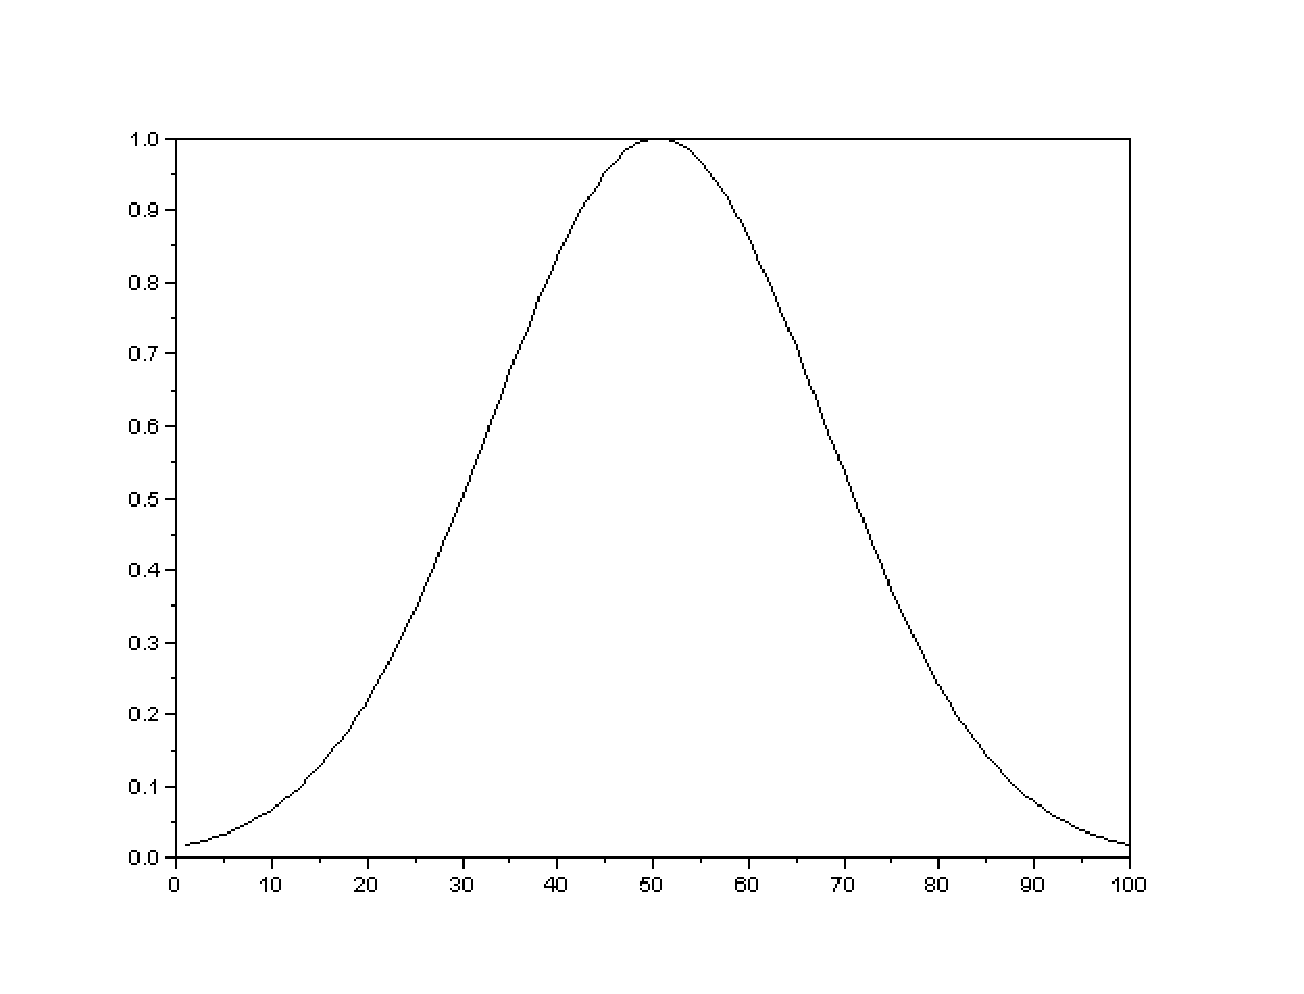
\includegraphics[width=12cm]{pics/maxwell_dist.eps}\\
\caption{Maxwell Distribution}\label{fig_maxwell}
\end{figure}

\begin{figure}
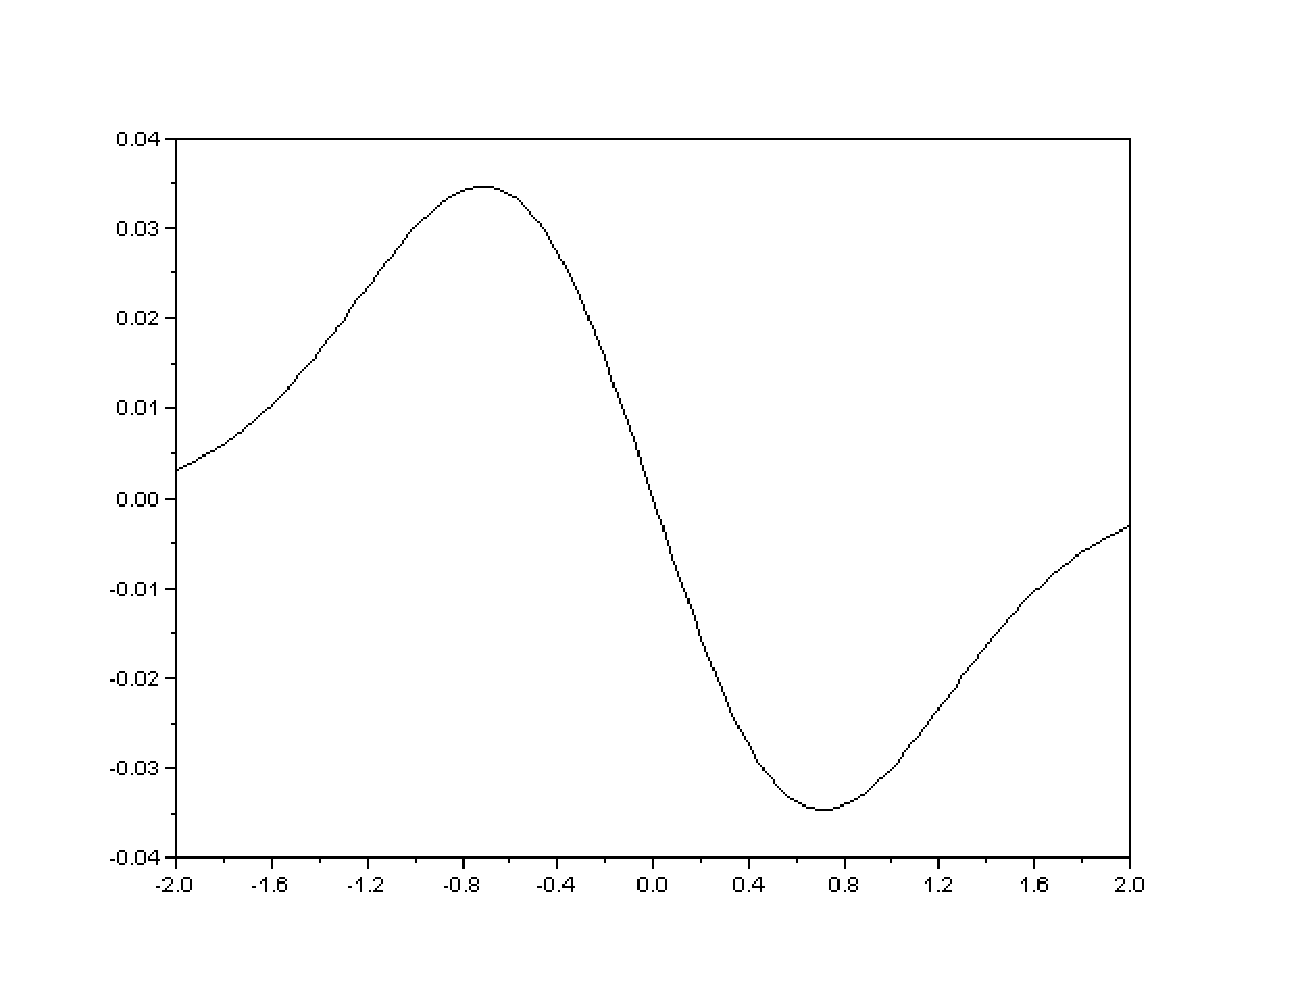
\includegraphics[width=12cm]{pics/maxwell_dist_diff.eps}\\
\caption{Derivative of Maxwell Distribution}\label{fig_maxwell_diff}
\end{figure}

\begin{figure}
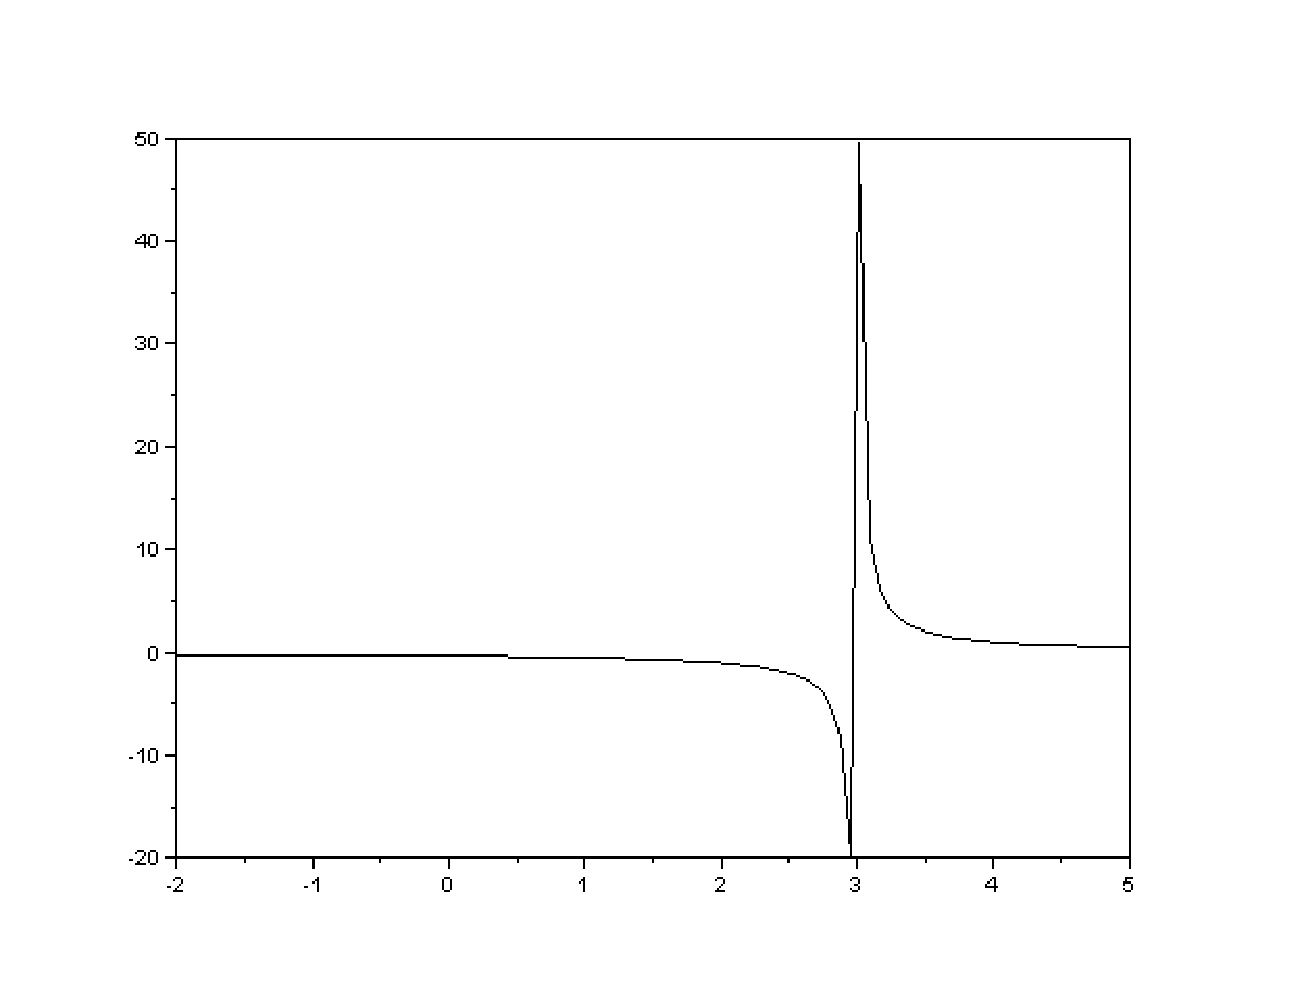
\includegraphics[width=12cm]{pics/nenner.eps}\\
\caption{Denominator of the integral:omega/k=3}\label{fig_denominator}
\end{figure}

So the numerator and the denominator of the kernel of the integral are prominent in different regions of the range of the velocity, as long as the maximum of F and $\frac{\omega}{k}$ are far enough apart. Then we can divide the integral in two parts, where the boundary is half way between max(v) and $\frac{\omega}{k}$. I call this speed $v_{sep}$.

\begin{eqnarray}
I &=& I_1 +I_2 \label{sep_int} \\
I_1 &=& \int^{v_{sep}}_{-\infty }{  \frac{\frac{\partial F}{\partial v}}{v-\frac{\omega}{k}} dv} \\
I_2 &=& \int^{\infty}_{v_{sep} }{  \frac{\frac{\partial F}{\partial v}}{v-\frac{\omega}{k}} dv}
\end{eqnarray}

\subsubsection{Ad Integral 1:}
In the part of the region, where the differential of F is prominent, $|\frac{k v}{\omega}|$ is small. Here we can approximate the denominator.

\begin{equation}
\left( 1-\frac{k v}{\omega} \right)^{-1}=1+ \frac{k v}{\omega} + \left( \frac{k v}{\omega} \right)^2 ...
\end{equation}

Hence

\begin{equation}
I_1=-\frac{k}{\omega} \left( \int^{\infty}_{-\infty } {\frac{\partial F}{\partial v}dv } + \frac{k}{\omega}\int^{\infty}_{-\infty } {\frac{\partial F}{\partial v} v dv }  + \frac{k^2}{\omega^2}\int^{\infty}_{-\infty } {\frac{\partial F}{\partial v} v^2 dv } + ...\right)
\end{equation}

By partial integration one gets

\begin{eqnarray}    I_1&=&-\frac{k}{\omega} \left[ F \right]^{\infty}_{-\infty } \\
&-& \frac{k^2}{\omega^2} \left[ F v \right]^{\infty}_{-\infty } +  \frac{k^2}{\omega^2} \int^{\infty}_{-\infty } F dv \nonumber \\
&-& \frac{k^3}{\omega^3} \left[ F v^2 \right]^{\infty}_{-\infty } +  \frac{2 k^3}{\omega^3} \int^{\infty}_{-\infty } Fv dv \nonumber \\
&-& \frac{k^4}{\omega ^4} \left[ F v^3 \right]^{\infty}_{-\infty } +  \frac{3 k^4}{\omega^4} \int^{\infty}_{-\infty } Fv^2 dv - ... \nonumber
\end{eqnarray}

Since F is zero at plus or minus infinity, we can set all negative terms to zero.

\begin{eqnarray}
I_1&=& \frac{k^2}{\omega^2} \int^{\infty}_{-\infty } F dv  \\
&+& \frac{2 k^3}{\omega^3} \int^{\infty}_{-\infty } Fv dv \nonumber \\
&+&   \frac{2 k^4}{\omega^4} \int^{\infty}_{-\infty } Fv^2 dv + ...\nonumber
\end{eqnarray}

$Fv$ is an even function, so this integral (and all even integrals of higher order) is(are) also zero. The following equation remains.

\begin{eqnarray}
I_1&=& \frac{k^2}{\omega^2} \int^{\infty}_{-\infty } F dv + \frac{3 k^4}{\omega^4} \int^{\infty}_{-\infty } {Fv^2 dv} + ... \\ &=& \frac{k^2}{\omega^2}  + \frac{3 k^4}{\omega^4} \bar{v^2} + ...\label{result_I1}
\end{eqnarray}

\subsubsection{Ad Integral 2:}
If we look at the diagrams, we realize that $\frac{\partial F}{\partial v}$ does not change its value much near $v=\frac{\omega}{k}$, where the denominator of the kernel is zero. So we take the derivative as a constant and set the integration range from $\frac{\omega}{k}- \left( \frac{\omega}{k}- v_{sep} \right)$ to $\frac{\omega}{k}+\left( \frac{\omega}{k}- v_{sep} \right)$.

\begin{equation}
I_2= \frac{\partial F}{\partial v}\mid_{v=\frac{\omega}{k}} \int^{2\frac{ \omega}{k} - v_{sep} }_{v_{sep}} {\left( v-\frac{\omega}{k} \right)^{-1} dv }
\end{equation}

Since $\omega$ is in general complex, we can split this integral in its real and imaginary part.

\begin{eqnarray}
I_3 &=& \int^{2\frac{ \omega}{k} - v_{sep}}_{v_{sep}} {\left( v-\frac{\omega_r}{k} -i\frac{\omega_i}{k}\right)^{-1} dv } \\
&=& \int^{2\frac{ \omega}{k} - v_{sep}}_{v_{sep}}{\frac{v-\frac{\omega_r}{k}}{\left( v-\frac{\omega_r}{k} \right)^2+\left( \frac{\omega_i}{k} \right)^2} dv } +  \frac{i\omega_i}{k}\int^{2\frac{ \omega}{k} - v_{sep}}_{v_{sep}}{\frac{1}{\left( v-\frac{\omega_r}{k} \right)^2+\left( \frac{\omega_i}{k} \right)^2} dv } \\
&=& I_r+I_i
\end{eqnarray}

$I_r$ is even about $v=\frac{\omega}{k}$, so it vanishes. For $I_i$ we substitute $x=v-\frac{\omega_r}{k}$ and get the standard integral

\begin{eqnarray}
I_i&=&\frac{i\omega_i}{k} \int^{+(\frac{\omega_r}{k}- v_{sep})}_{-(\frac{\omega_r}{k}- v_{sep})}{\frac{1}{x^2+\frac{\omega_i^2}{k^2}}dx} \\
&=& \frac{i\omega_i}{k} \left[ \frac{k}{\omega_i} \arctan{\frac{x}{\frac{\omega_i}{k}}}\right]_{-(\frac{\omega_r}{k}- v_{sep})}^{+(\frac{\omega_r}{k}- v_{sep})}\\
&=& i \left[ \arctan{\frac{x}{\frac{\omega_i}{k}}}\right]_{-(\frac{\omega_r}{k}- v_{sep})}^{+(\frac{\omega_r}{k}- v_{sep})} \\ &=& i \left[ \arctan \left(\frac{+(\frac{\omega_r}{k}- v_{sep})}{\frac{\omega_i}{k}}\right) - \arctan \left( \frac{-(\frac{\omega_r}{k}- v_{sep})}{\frac{\omega_i}{k}}\right) \right]
\end{eqnarray}

Since the real part of the frequency is far greater than the imaginary part, we can extend the boundary of the integral to plus and minus infinity.

\begin{eqnarray}
I_i&=& i \left[ \arctan {(\infty)} - \arctan {(-\infty)} \right]\\
&=& i \pi
\end{eqnarray}

Hence

\begin{equation}
I_3=i \pi
\end{equation}

and

\begin{equation}\label{result_I2}
I_2=i \frac{\partial F}{\partial v}\mid_{v=\frac{\omega}{k}} \pi
\end{equation}

From equations (\ref{dispersion_relation2}), (\ref{result_I1}) and (\ref{result_I2}), we get

\begin{equation}\label{dispersion_relation_solved}
\frac{ \omega_p^2}{ k^2}  (I_1+I_2) =1
\end{equation}

or

\begin{equation}\label{dispersion_relation_solved_2}
\frac{ \omega_p^2}{ k^2}  \left[ \left(\frac{k^2}{\omega^2}  + \frac{3 k^4}{\omega^4} \bar{v^2} \right)+ \left(i \frac{\partial F}{\partial v}\mid_{v=\frac{\omega}{k}} \pi \right) \right] =1
\end{equation}

I dismissed all terms of higher order in the solution of $I_2$. To get a valid dispersion relation, we have to isolate $\omega$.

\begin{eqnarray}
\omega^2 &=&  \omega_p^2  \left[ \left( 1  + \frac{3 k^2}{\omega^2} \bar{v^2} \right)+ \frac{\omega^2}{k^2}\left(i \frac{\partial F}{\partial v}\mid_{v=\frac{\omega}{k}} \pi \right) \right]\\
\omega^2 &=& \omega_p^2 + \omega_p^2 \left[ \frac{3 k^2}{\omega^2} \bar{v^2} + \frac{\omega^2}{k^2}\left(i \frac{\partial F}{\partial v}\mid_{v=\frac{\omega}{k}} \pi \right) \right]
\end{eqnarray}

This equation requires a complex $\omega$. As we postulated at the beginning of the derivation, the disturbance is proportional to

\begin{equation}
e^{-i \omega t}=e^{-i \omega_r t}e^{ \omega_i t}
\end{equation}

So the imaginary part of the frequency controls the excitation or damping of the wave, depending on its sign. Its sign, in turn, depends on the sign of the slope of the distribution function at the point $\frac{\omega}{k}$. In case of a Maxwell distribution, the slope is negative, which corresponds to a damping situation. This damping is called \emph{Landau damping}.

\subsection{Two fluid instability}
\begin{figure}
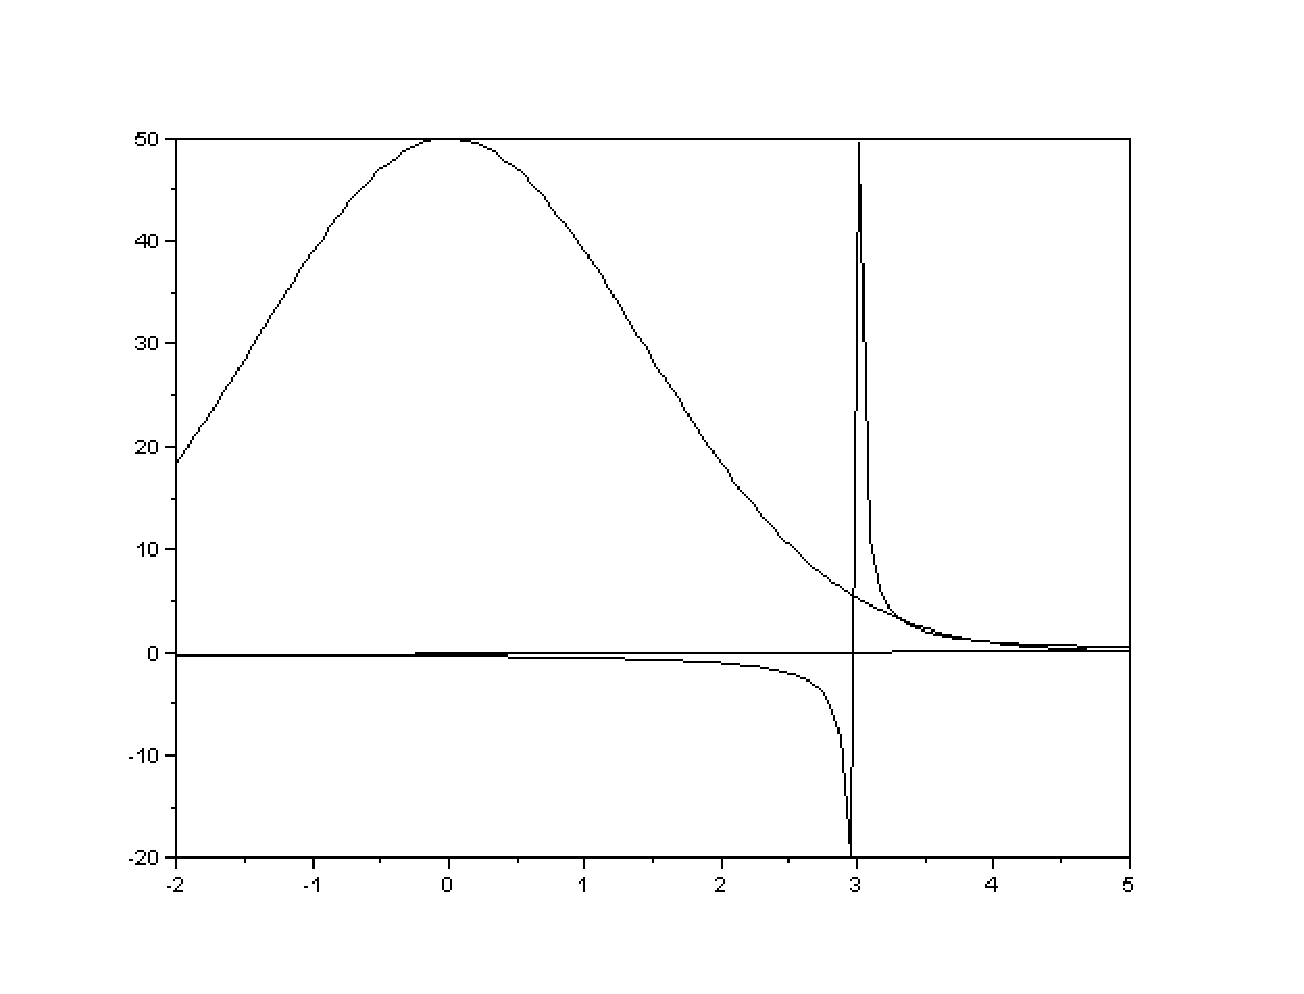
\includegraphics[width=12cm]{pics/maxwell_dist2.eps}\\
\caption{Maxwell Distribution and the denominator of the integral kernel}\label{fig_maxwell2}
\end{figure}

\begin{figure}
    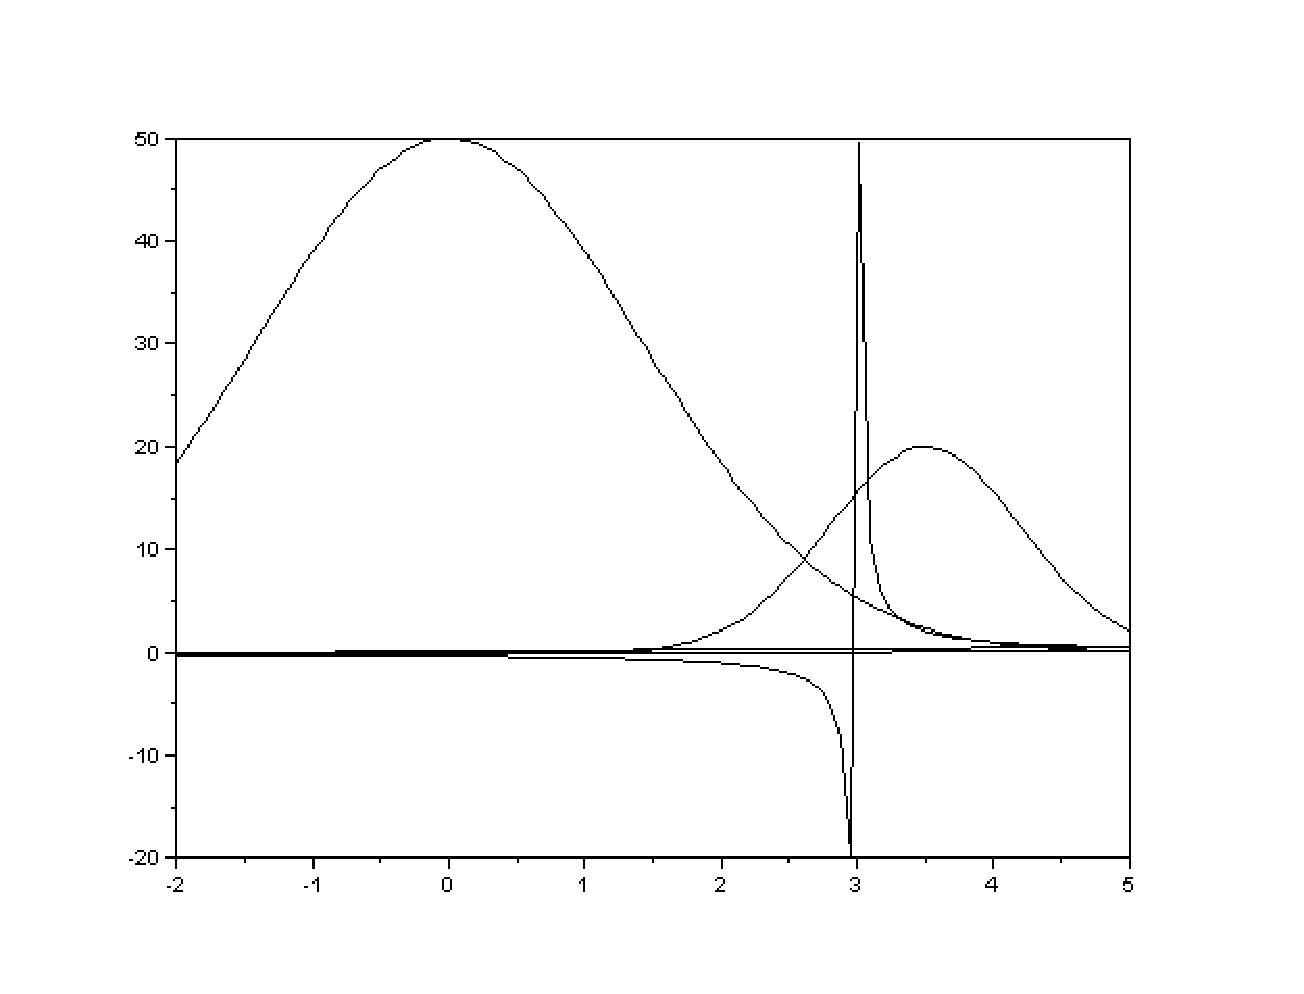
\includegraphics[width=12cm]{pics/twofluids_saperated.eps}\\
    \caption{Maxwell Distribution of two fluids and the denominator of the integral kernel}\label{fig_2fluids_sep} \end{figure}

\begin{figure}
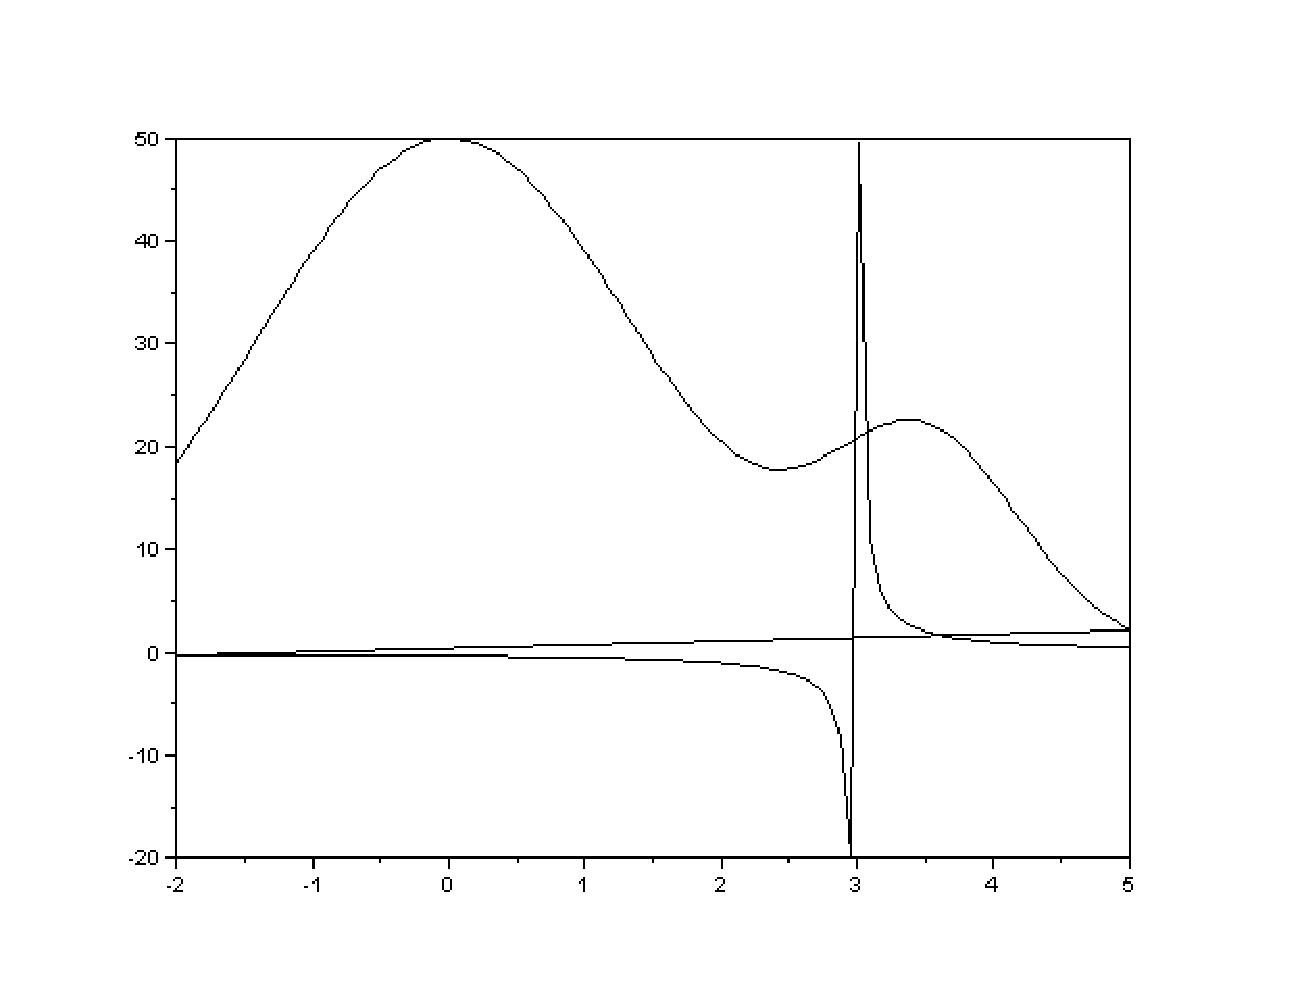
\includegraphics[width=12cm]{pics/twofluids_added.eps}\\
\caption{Combined Maxwell Distribution of two fluids and the denominator of the integral kernel}\label{fig_2fluids_added}
\end{figure}

As we said in the last subsection, the slope of the velocity distribution function is normally negative, which correspond to damping. But can there be a situation where excitation happens ? The answer is \emph{yes}. I can think of two such situations. The first one is if a second fluid moved through the first one (for instance an electron beam) and has a bulk velocity that is just a little bit greater than $\frac{\omega}{k}$. Then the two distribution functions add, as can be seen in the diagrams \ref{fig_maxwell2} - \ref{fig_2fluids_added}. The slope at the relevant point is now positive. This is a situation that can not be described by two fluid theory. There is an energy transfer from the electron beam to the underlying fluid, by electrostatic waves, without need of collisions as in normal hydrodynamics.

\subsection{Cyclotron maser Instability} The second scenario, I want to mention is the cyclotron maser instability. Here, the distribution function is thinned out at the right velocity, because particles with this certain speed are absorbed by a planetary atmosphere. This may happen when particles are trapped in the radiation belt of the planetary magnetic field. Particles which have a certain velocity component along the magnetic field lines can travel into the high atmosphere of the planet in the auroral region. The probability is high, that they collide with an atmospheric particle, due to the high density in this region. If this happens they are lost for the plasma of the radiation belt, so the distribution function decreases in the opposite direction, where the absorbed particles fail to return after undergoing the mirror process.

\subsection{Qualitative physical description of Landau damping} \cite{jackson} gives an interesting, physical description of Landau damping. He describes the damping process a result of an energy transfer from the wave to the particles. When the wave is sufficiently slow, particles are trapped in the wave and will move along with the wave. For this to happen, the faster particles have to be slowed down, the particles that are slower than the speed of the wave, are accelerated. In a normal Maxwell distribution, there are always more slower particles than faster particles, so more particles gain energy than loose energy. This net energy gain is removed from the energy of the wave. It is dampened. Only when the gradient is reversed, there can be the case that there are more particles around to be slowed down. This would  lead to the excitation of the wave.

\chapter{Wave zoology}
\section{MHD waves}
\begin{table}[h]
\label{tab_mhd_waves}
\caption{MHD Wave zoology}
\begin{tabular}{|c|c|c|c|c|}
  \hline
% after \\: \hline or \cline{col1-col2} \cline{col3-col4} ...
\textbf{Name} & \textbf{Characteristics} & \textbf{Dispersion relation} & \textbf{Phase speed}  \\
\hline
Alfven Waves & transversal, $k \| B_0$, inkompressible & $k^2 =  \frac{\omega^2 \rho_0 \mu_0}{B_{0}^2}$ & $\frac{B_{0,x}^2}{\sqrt{ \rho_0 \mu_0}}$  \\
MHD Compression Waves & longitudinal, $k \bot B_0$  &  $\omega  =   k \sqrt{v_s^2  +   v_A^2}$ & $\sqrt{v_s^2  +   v_A^2}$ \\
x & x & x & x  \\
x & x & x & x  \\
\hline\end{tabular}
\end{table}

\begin{table}[h]
\label{tab_mhd_waves2}
\caption{MHD Wave zoology 2}
\begin{tabular}{|c|c|c|}
  \hline
% after \\: \hline or \cline{col1-col2} \cline{col3-col4} ...
\textbf{Name} & \textbf{Frequency range in IMF} & \textbf{Can exist in IMF ?} \\
\hline
Alfven Waves & x & yes \\
MHD Compression Waves &  x & yes \\
x & x & x \\
x & x & x  \\
\hline\end{tabular}
\end{table}

\section{Kinetic waves}
\begin{table}[h]
\label{tab_kinetic_waves}
\caption{Kinetic Wave zoology}
\begin{tabular}{|c|c|c|c|}
  \hline
% after \\: \hline or \cline{col1-col2} \cline{col3-col4} ...
\textbf{Name} & \textbf{Characteristics} & \textbf{Dispersion relation} & \textbf{Phase speed} \\
\hline
Langmuir Waves &  & $\omega_l^2=\omega_p^2+k^2\gamma_ev_{the}^2$ & $\sqrt{\frac{\omega_p^2}{k^2}+\gamma_ev_{the}^2}$ \\
x & x & x & x  \\
x & x & x & x  \\
\hline\end{tabular}
\end{table}

\begin{table}[h]
\label{tab_kinetic_waves2}
\caption{Kinetic Wave zoology 2}
\begin{tabular}{|c|c|c|}
  \hline
\textbf{Name} & \textbf{Frequency range in IMF} & \textbf{Can exist in IMF ?} \\
\hline
Langmuir Waves &  x & yes \\
x & x & x \\
x & x & x  \\
\hline\end{tabular}
\end{table}

\part{EM waves in plasma}
\chapter{Frequency dispersion characteristics}
\section{General}
The 1D equation of motion for an isolated electron is

\begin{equation}
    m_e \left[\ddot{x} +\gamma \dot{x}+\omega_p x \right]=-e E
\end{equation}

$\gamma$ corresponds to a damping constant. When the exciting field is harmonic, one can solve this equation to give

\begin{equation}
    x=-\frac{e E}{m_e(\omega_p^2 -\omega^2 -\imath \omega \gamma)}
\end{equation}

So the dipole moment is

\begin{equation}
    p=-ex=\frac{e^2 E}{m_e(\omega_p^2 -\omega^2 -\imath \omega \gamma)}
\end{equation}

Further

\begin{equation}
    P=(\varepsilon-1)\varepsilon_0 E
\end{equation}

so

\begin{eqnarray}
    \frac{e^2 E}{m_e(\omega_p^2 -\omega^2 -\imath \omega \gamma)}&=&(\varepsilon-1)\varepsilon_0 E\\
(\varepsilon-1)\varepsilon_0&=& \frac{e^2 }{m_e(\omega_p^2 -\omega^2 -\imath \omega \gamma)}\\
\varepsilon&=& 1+\frac{e^2 }{ \varepsilon_0 m_e(\omega_p^2 -\omega^2 -\imath \omega \gamma)}
\end{eqnarray}

The imaginary part of the permittivity can be positive (attenuation) or negative (amplification). In case of free electrons ($\omega_p \rightarrow 0$) the equation becomes

\begin{equation}
    \varepsilon= 1+\frac{e^2 }{ \varepsilon_0 m_e(\omega^2  -\imath \omega \gamma)}
\end{equation}

In \cite{my_masterthesis} I find


\begin{equation}
\label{epsilon_plasma}    \varepsilon=\varepsilon_0 \left(1-\frac{\omega_p^2 }{ \omega^2 }\right)
\end{equation}

for unmagnetized plasma, which is the high frequency limit. The dispersion relation is then

\begin{equation}
k^2=\omega^2\mu_0\varepsilon_0 \left(1-\frac{\omega_p^2 }{ \omega^2 }\right)
\end{equation}

When the frequency of the EM wave is smaller than the plasma frequency, the wave number is imaginary. The wave is reflected and the field strengths decrease exponentially. When the frequency is larger than the plasma frequency, the wave number is real, so there is no net energy flow between wave and plasma.

\section{The Maxwell equations in Matter}
\begin{eqnarray}
% \nonumber to remove numbering (before each equation)
  \nabla \cdot \mathbf{D} &=& 0 \\
\nabla \times \mathbf{H}- \frac{\partial \mathbf{D}}{\partial t}&=&  0\\
\nabla \times \mathbf{E} + \frac{\partial \mathbf{B}}{\partial t} &=& 0 \\
\nabla \cdot \mathbf{B} &=& 0
\end{eqnarray}

The sources inside the matter are included in the dielectric tensor. One can define external sources, like the charges and currents of an antenna. Then the equations can look like

\begin{eqnarray}
% \nonumber to remove numbering (before each equation)
  \nabla \cdot \mathbf{D} &=& \rho_{ant} \\
\nabla \times \mathbf{H}- \frac{\partial \mathbf{D}}{\partial t}&=& \mathbf{j}_{ant} \\
\nabla \times \mathbf{E} + \frac{\partial \mathbf{B}}{\partial t} &=& 0 \\
\nabla \cdot \mathbf{B} &=& 0
\end{eqnarray}


\section{The Boundary Conditions}

\begin{eqnarray}
% \nonumber to remove numbering (before each equation)
  \mathbf{n}\times \Delta \mathbf{E} &=& 0 \\
\mathbf{n} \cdot \Delta\mathbf{B} &=& 0 \\
\mathbf{n}\times (\mathbf{H}_2-\mathbf{H}_1) &=& \mathbf{j}_s \\
\mathbf{n}\cdot (\mathbf{D}_2-\mathbf{D}_1) &=& \sigma \\
\end{eqnarray}
\section{Dielectric tensor}
\subsection{Cold plasma approximation}
In \cite{my_masterthesis} I derived the dielectric tensor for cold magnetized plasma. The direction of the external magnetic field is the z-axis.

 \begin{equation}
 \label{gyrotropic_tensor}
 \bar{\varepsilon}=\varepsilon_0\left(%
 \begin{array}{ccc}
 K' & iK'' & 0 \\
 -iK'' & K' & 0 \\
 0 & 0 & K_0 \\
 \end{array}
  \right)
  \end{equation}

where

\begin{eqnarray}
 K' &=& 1-\frac{UX}{U^2-Y^2} \\
 K'' &=&- \frac{XY}{U^2-Y^2} \\
 K_0 &=& 1-\frac{X}{U} \\
 U &=&  1-\frac{i\nu}{\omega}\\
 X &=&  \frac{\omega_p^2}{\omega^2}\\
 Y &=& \frac{\omega_c}{\omega}
 \end{eqnarray}

 $\nu$ is the electron collision frequency.

so

\begin{equation}
 \label{gyrotropic_tensor2}
 \bar{\varepsilon}=\varepsilon_0\left(%
 \begin{array}{ccc}
 1-\frac{UX}{U^2-Y^2} & -i \frac{XY}{U^2-Y^2} & 0 \\
 i \frac{XY}{U^2-Y^2} & 1-\frac{UX}{U^2-Y^2} & 0 \\
 0 & 0 & 1-\frac{X}{U} \\
 \end{array}
  \right)
  \end{equation}

or in detail

\begin{equation}
 \label{gyrotropic_tensor3}
 \bar{\varepsilon}=\varepsilon_0\left(%
 \begin{array}{ccc}
 1-\frac{(1-\frac{i\nu}{\omega}) \frac{\omega_p^2}{\omega^2}}{(1-\frac{i\nu}{\omega})^2-(\frac{\omega_c}{\omega})^2} & -i \frac{ \frac{\omega_p^2}{\omega^2}\frac{\omega_c}{\omega}}{(1-\frac{i\nu}{\omega})^2-(\frac{\omega_c}{\omega})^2} & 0 \\
 i \frac{ \frac{\omega_p^2}{\omega^2}\frac{\omega_c}{\omega}}{(1-\frac{i\nu}{\omega})^2-(\frac{\omega_c}{\omega})^2} & 1-\frac{(1-\frac{i\nu}{\omega}) \frac{\omega_p^2}{\omega^2}}{(1-\frac{i\nu}{\omega})^2-(\frac{\omega_c}{\omega})^2} & 0 \\
 0 & 0 & 1-\frac{ \frac{\omega_p^2}{\omega^2}}{1-\frac{i\nu}{\omega}} \\
 \end{array}
  \right)
  \end{equation}


 When the plasma can be treated as collisionless ($\nu=0\rightarrow U=1$), the equation can be simplified.

  \begin{eqnarray}
  K' &=& 1-\frac{X}{1-Y^2} = 1-\frac{\omega_p^2}{\omega^2-\omega_c^2}\\
  K'' &=& -\frac{XY}{1-Y^2} = -\frac{\omega_p^2 \omega_c}{\omega(\omega^2-\omega_c^2)}\\
  K_0 &=& 1-\frac{\omega_p^2}{\omega^2}
\end{eqnarray}

So


\begin{equation}
 \label{gyrotropic_tensor3_collless}
 \bar{\varepsilon}=\varepsilon_0\left(%
 \begin{array}{ccc}
 1-\frac{\omega_p^2}{\omega^2 -\omega_c^2} & -i\frac{\omega_p^2 \omega_c}{\omega(\omega^2-\omega_c^2)} & 0 \\
 i \frac{\omega_p^2 \omega_c}{\omega(\omega^2-\omega_c^2)} & 1-\frac{\omega_p^2}{\omega^2 -\omega_c^2} & 0 \\
 0 & 0 & 1-\frac{\omega_p^2}{\omega^2} \\
 \end{array}
  \right)
  \end{equation}

Generalized for different particle species s, it is

\begin{equation}
 \label{gyrotropic_tensor3_collless_multi_comp}
 \bar{\varepsilon}=\varepsilon_0\left(%
 \begin{array}{ccc}
 1-\sum_s \frac{\omega_{p,s}^2}{\omega^2 -\omega_{c,s}^2} & - \imath \sum_s \frac{\omega_{p,s}^2 \omega_{c,s}}{\omega(\omega^2-\omega_{c,s}^2)} & 0 \\
 \imath \sum_s \frac{\omega_{p,s}^2 \omega_{c,s}}{\omega(\omega^2-\omega_{c,s}^2)} & 1- \sum_s \frac{\omega_{p,s}^2}{\omega^2 -\omega_{c,s}^2} & 0 \\
 0 & 0 & 1- \sum_s \frac{\omega_{p,s}^2}{\omega^2} \\
 \end{array}
  \right)
  \end{equation}

When, additionally, $B_0\rightarrow 0$, the gyration frequency approaches zero and the gyrotropic tensor becomes an isotropic tensor, as in unmagnetized plasma.

 \begin{equation}\label{isotropic_tensor}
 \bar{\varepsilon}=\varepsilon_0
 \left(
 \begin{array}{ccc}
 1-\frac{\omega_p^2}{\omega^2} & 0 & 0 \\
 0 & 1-\frac{\omega_p^2}{\omega^2} & 0 \\
 0 & 0 & 1-\frac{\omega_p^2}{\omega^2}
 \\\end{array}
  \right)
  \end{equation}

  The other extremum is that the external magnetic field is very strong. Then the tensor becomes \emph{uniaxial}.

  \begin{equation}\label{isotropic_tensor}
  \bar{\varepsilon}=\varepsilon_0
  \left(
   \begin{array}{ccc}  1 & 0 & 0 \\
   0 & 1 & 0 \\
   0 & 0 & 1-\frac{\omega_p^2}{\omega^2} \\
   \end{array}
    \right)
    \end{equation}


\subsection{The Stix notation}
Tensors (\ref{gyrotropic_tensor3}) and (\ref{gyrotropic_tensor3_collless}) can be written in a way such that they include left and right handed polarization separately. First (\ref{gyrotropic_tensor3_collless}).

\begin{equation}
 \bar{\varepsilon}=\varepsilon_0\left(%
 \begin{array}{ccc}
 1-\frac{\omega_p^2}{(\omega +\omega_c)(\omega -\omega_c)} & -i\frac{\omega_p^2 \omega_c}{\omega(\omega+\omega_c)(\omega-\omega_c)} & 0 \\
 i \frac{\omega_p^2 \omega_c}{\omega(\omega+\omega_c)(\omega-\omega_c)} & 1-\frac{\omega_p^2}{(\omega +\omega_c)(\omega -\omega_c)} & 0 \\
 0 & 0 & 1-\frac{\omega_p^2}{\omega^2} \\
 \end{array}
  \right)
  \end{equation}

or

\begin{equation}
 \bar{\varepsilon}=\varepsilon_0\left(%
 \begin{array}{ccc}
 1-\left( \frac{\omega_p^2}{\omega (\omega +\omega_c)}+\frac{\omega_p^2}{\omega (\omega -\omega_c)} \right) & -i\left( \frac{\omega_p^2}{\omega (\omega +\omega_c)}-\frac{\omega_p^2}{\omega (\omega -\omega_c)} \right) & 0 \\
 i \left( \frac{\omega_p^2}{\omega (\omega +\omega_c)}-\frac{\omega_p^2}{\omega (\omega -\omega_c)} \right) & 1-\left( \frac{\omega_p^2}{\omega (\omega +\omega_c)}+\frac{\omega_p^2}{\omega (\omega -\omega_c)} \right) & 0 \\
 0 & 0 & 1-\frac{\omega_p^2}{\omega^2} \\
 \end{array}
  \right)
  \end{equation}


$\omega+\omega_c$ corresponds to right handed polarization, while $\omega-\omega_c$ corresponds to left handed polarization, depending on convention. We can define

\begin{eqnarray}
% \nonumber to remove numbering (before each equation)
  S &=& \frac{1}{2}(R+L) \\
D &=& \frac{1}{2}(R-L) \\
R &=& 1+ \chi^- = 1- \frac{\omega_p^2}{\omega (\omega +\omega_c)} \\
L &=& 1+ \chi^+ =1-\frac{\omega_p^2}{\omega (\omega -\omega_c)}\\
P&=& 1-\frac{\omega_p^2}{\omega^2}
\end{eqnarray}

Then the tensor can be written as


\begin{equation}
 \label{gyrotropic_tensor}
 \bar{\varepsilon}=\varepsilon_0\left(%
 \begin{array}{ccc}
 S & -iD & 0 \\
 iD & S & 0 \\
 0 & 0 & P \\
 \end{array}
  \right)
  \end{equation}


$\chi$ is the susceptibility and is additive. Therefor the susceptibilities of the different particle species s can simply be added together.


\begin{eqnarray}
R &=& 1+ \sum \chi_s^- = 1- \sum \frac{\omega_{p,s}^2}{\omega (\omega +\omega_{c,s})} \\
L &=& 1+ \sum \chi_s^+ =1-\sum \frac{\omega_{p,s}^2}{\omega (\omega -\omega_{c,s})}\\
P&=& 1- \sum \frac{\omega_{p,s}^2}{\omega^2}
\end{eqnarray}

\subsection{the general dispersion relation}
The dielectric tensor can be used to establish a general dispersion relation that can be used to find the different wave modi. I have to use the Maxwell equations for media.


\begin{eqnarray}
% \nonumber to remove numbering (before each equation)
  \nabla \cdot \mathbf{D} &=& 0 \\
\nabla \times \mathbf{H}- \frac{\partial \mathbf{D}}{\partial t}&=&  0\label{maxwell2} \\
\nabla \times \mathbf{E} + \frac{\partial \mathbf{B}}{\partial t} &=& 0 \label{maxwell3} \\
\nabla \cdot \mathbf{B} &=& 0
\end{eqnarray}

Postulating a harmonic behavior and Fourier transforming (\ref{maxwell2}) and (\ref{maxwell3}), I get

\begin{eqnarray}
 \mathbf{k} \times \mathbf{E}&=&  \omega \mathbf{B}  \\
 \mathbf{k} \times \mathbf{H}&=& -\omega \mathbf{D}
\end{eqnarray}

These equations can be further combined to give

\begin{eqnarray}
 \mathbf{k} \times \mathbf{E}&=&  \omega \mathbf{B}  \\
 \mathbf{k} \times \mathbf{B}&=& -\omega \mu \mathbf{D}\\
\rightarrow \mathbf{k} \times\mathbf{k} \times  \mathbf{E} + \omega^2 \mu \mathbf{D} &=&0
\end{eqnarray}

or

\begin{equation}
    \mathbf{k} \times\mathbf{k} \times  \mathbf{E} + \omega^2 \mu \varepsilon_0 \mathbf{\varepsilon} \cdot \mathbf{E} =0
\end{equation}

Defining $n=\frac{\mathbf{k}}{\omega \sqrt{\mu_0 \varepsilon_0}}=\frac{\mathbf{k}c}{\omega}$, I can write

\begin{equation}
    \mathbf{n} \times\mathbf{n} \times  \mathbf{E} +  \mathbf{\epsilon} \cdot \mathbf{E} =0
\end{equation}


Attenzione !!! I made two important things in this transformation: I assumed that $\mu=\mu_0$ and I drew the permittivity of free space out of the epsilon tensor. I also use an other epsilon to allow for this change. The first assumption is valid for plasma, since the gyration effect is completely described by the permittivity tensor.\\

Using

\begin{equation}
    \mathbf{n} \times \mathbf{n} \times \mathbf{E} = \mathbf{n}\mathbf{n} \mathbf{E}- \mathbf{n}^2 \mathbf{E}
\end{equation}

I get

\begin{equation}
    \mathbf{n}\mathbf{n} \mathbf{E}- \mathbf{n}^2   \mathbf{E} +  \mathbf{\epsilon} \cdot \mathbf{E} =0
\end{equation}

or

\begin{equation}
    (\mathbf{n}\mathbf{n} - \mathbf{n}^2\mathbf{I}  +  \mathbf{\epsilon} ) \mathbf{E} =0
\end{equation}

 So I can define a Radiation tensor \textbf{T} to write the equation, governing \textbf{E}, in concise form:

\begin{equation}
    \mathbf{T}\cdot \mathbf{E}=0
\end{equation}

where

\begin{eqnarray}
    \mathbf{T}&=&\left(%
\begin{array}{ccc}
   n_1^2 -\mathbf{n}^2 &  n_1 n_2 & n_1 n_3 \\
n_1 n_2 & n_2^2 -\mathbf{n}^2 & n_2 n_3 \\
 n_1 n_3  &  n_2 n_3  &  n_3^2-\mathbf{n}^2 \\
\end{array}%
\right)+\left(%
 \begin{array}{ccc}
 S & -\imath D & 0 \\
 \imath D & S & 0 \\
 0 & 0 & P \\
 \end{array}
  \right)\\
&=&
\left(%
\begin{array}{ccc}
   n_1^2 -\mathbf{n}^2 +S &  n_1 n_2-\imath D & n_1 n_3 \\
n_1 n_2 +\imath D& n_2^2 -\mathbf{n}^2+S & n_2 n_3 \\
 n_1 n_3  &  n_2 n_3  &  n_3^2-\mathbf{n}^2+P \\
\end{array}%
\right)
\end{eqnarray}

Assuming that the n vector is in the 1-3 plane:

\begin{eqnarray}
    \mathbf{T}&=&
\left(%
\begin{array}{ccc}
   n_1^2 -\mathbf{n}^2 +S &  -\imath D & n_1 n_3 \\
 \imath D&  -\mathbf{n}^2+S &  0\\
 n_1 n_3  &  0  &  n_3^2-\mathbf{n}^2+P \\
\end{array}%
\right)
\end{eqnarray}

Transforming the tensor into a spherical coordinate system, where




\begin{eqnarray}
% \nonumber to remove numbering (before each equation)
  n1 &=& n\sin(\theta)\cos(\phi) \\
n2 &=&  n\sin(\theta) \sin(\phi)\\
n3 &=&  n\cos(\theta)
\end{eqnarray}

we get

\begin{eqnarray}
    \mathbf{T}&=&
\left(%
\begin{array}{ccc}
   n^2\sin^2(\theta) - n^2 +S &  -\imath D &n^2 \sin(\theta) \cos(\theta) \\
 \imath D&  -n^2+S & 0 \\
n^2 \sin(\theta) \cos(\theta)  &  0  & n^2 \cos(\theta)^2-n^2+P \\
\end{array}%
\right)\\
&=&
\left(%
\begin{array}{ccc}
     S-n^2\cos^2(\theta) &  -\imath D &n^2 \sin(\theta) \cos(\theta) \\
 \imath D&  S-n^2 & 0 \\
n^2 \sin(\theta) \cos(\theta)  &  0  & P-n^2 \sin^2(\theta) \\
\end{array}%
\right)
\end{eqnarray}




$\theta $ is the angle between the z axis, which is also the direction of the external magnetic field, and the direction \textbf{n}, which is also the direction of \textbf{k}. Since the equation has no source terms, it can be solved by setting the determinant of the tensor equal to zero. This produces the dispersion relations of the wave modi. The equation is universal, when shifting to plasma with collisions or temperate plasma, one has only to change the dielectric tensor. At low frequency, the nonlocality in space can be ignored.

\subsection{Hot plasma}

\section{The dyadic Green's function}
On base of the Maxwell equations in matter

\begin{eqnarray}
% \nonumber to remove numbering (before each equation)
  \nabla \cdot \mathbf{D} &=& \rho_{ant} \\
\nabla \times \mathbf{H}- \frac{\partial \mathbf{D}}{\partial t}&=& \mathbf{j}_{ant} \label{max2} \\
\nabla \times \mathbf{E} + \frac{\partial \mathbf{B}}{\partial t} &=& 0 \label{max3}\\
\nabla \cdot \mathbf{B} &=& 0
\end{eqnarray}

in combination with the constitutive relations

\begin{eqnarray}
    \mathbf{D}&=&\epsilon_0 \mathbf{\epsilon}\cdot \mathbf{E}\label{consti1}\\
\mathbf{B}&=& \mu_0 \cdot \mathbf{H}\label{consti2}
\end{eqnarray}

on can derive the wave equation by performing the rotation of (\ref{max3}).

\begin{eqnarray}
\nabla \times \nabla \times \mathbf{E} + \nabla \times \frac{\partial \mathbf{B}}{\partial t} &=& \\
\nabla \times \nabla \times \mathbf{E} +  \frac{\partial }{\partial t} (\nabla \times \mathbf{B}) &=& 0
\end{eqnarray}

With (\ref{max2}) and (\ref{consti2})

\begin{eqnarray}
\nabla \times \nabla \times \mathbf{E} +  \frac{\partial }{\partial t} (\mu_0 \frac{\partial \mathbf{D}}{\partial t}+ \mu_0 \mathbf{j}_{ant}) &=&\\
\nabla \times \nabla \times \mathbf{E}(\mathbf{r},t) +   \mu_0 \frac{\partial^2 \mathbf{D}(\mathbf{r},t)}{\partial t^2}+ \mu_0 \frac{\partial  \mathbf{j}_{ant}(\mathbf{r},t)}{\partial t} &=&0
\end{eqnarray}

Performing a Fourier transform with respect to time and using (\ref{consti1}) one gets

\begin{eqnarray}
\nabla \times \nabla \times \mathbf{E}(\mathbf{r},\omega) -   \mu_0 \omega^2 \mathbf{D}(\mathbf{r},\omega) - \mu_0 \imath \omega   \mathbf{j}_{ant}(\mathbf{r},\omega) &=& \\
\nabla \times \nabla \times \mathbf{E}(\mathbf{r},\omega) -   \mu_0 \epsilon_0 \omega^2 \mathbf{\epsilon}\cdot \mathbf{E}(\mathbf{r},\omega) - \mu_0 \imath \omega   \mathbf{j}_{ant}(\mathbf{r},\omega) &=&\nonumber \\
\nabla \times \nabla \times \mathbf{E}(\mathbf{r},\omega) -   k_0^2 \mathbf{\epsilon}\cdot \mathbf{E}(\mathbf{r},\omega) - \mu_0 \imath \omega   \mathbf{j}_{ant}(\mathbf{r},\omega) &=&0\nonumber
\end{eqnarray}

where $k_0^2=\mu_0 \epsilon_0 \omega^2$ We want to find the dyadic Green's function such that

\begin{equation}
    \mathbf{E}(\mathbf{r},\omega)=\int_V \mathbf{G}(\mathbf{r}-\mathbf{r'})\cdot \mathbf{j}_{ant}(\mathbf{r'},\omega) dV'
\end{equation}

so

\begin{eqnarray}
\nabla \times \nabla \times \int_V \mathbf{G}(\mathbf{r}-\mathbf{r'})\cdot \mathbf{j}(\mathbf{r'},\omega) dV' -   k_0^2 \mathbf{\epsilon}\cdot \int_V \mathbf{G}(\mathbf{r}-\mathbf{r'})\cdot \mathbf{j}(\mathbf{r'},\omega) dV' - \mu_0 \imath \omega   \mathbf{j}_{ant}(\mathbf{r},\omega) &=& 0
\end{eqnarray}


\begin{eqnarray}
\int_V \left( \nabla \times \nabla \times  \mathbf{G}(\mathbf{r}-\mathbf{r'}) -   k_0^2 \mathbf{\epsilon}\cdot  \mathbf{G}(\mathbf{r}-\mathbf{r'}) - \mu_0 \imath \omega \mathbf{I}  \delta (\mathbf{r}-\mathbf{r'}) \right)\cdot \mathbf{j}(\mathbf{r'},\omega) dV' &=& 0
\end{eqnarray}

\begin{eqnarray}
 \nabla \times \nabla \times  \mathbf{G}(\mathbf{r}-\mathbf{r'}) -   k_0^2 \mathbf{\epsilon}\cdot  \mathbf{G}(\mathbf{r}-\mathbf{r'})  &=& \mu_0 \imath \omega \mathbf{I}  \delta (\mathbf{r}-\mathbf{r'})
\end{eqnarray}

Using the identity

\begin{equation}
    \nabla \times \nabla \times \mathbf{G} = \nabla \nabla \mathbf{G}- \nabla^2 \mathbf{G}
\end{equation}

we get

\begin{eqnarray}
  \nabla \nabla \mathbf{G}(\mathbf{r}-\mathbf{r'})- \nabla^2 \mathbf{G}(\mathbf{r}-\mathbf{r'}) -   k_0^2 \mathbf{\epsilon}\cdot  \mathbf{G}(\mathbf{r}-\mathbf{r'})  &=& \mu_0 \imath \omega \mathbf{I}  \delta (\mathbf{r}-\mathbf{r'})\\
 \left( \nabla \nabla - \nabla^2 \mathbf{I} -   k_0^2 \mathbf{\epsilon}\right) \cdot  \mathbf{G}(\mathbf{r}-\mathbf{r'})  &=& \mu_0 \imath \omega \mathbf{I}  \delta (\mathbf{r}-\mathbf{r'})
\end{eqnarray}

$\left( \nabla \nabla - \nabla^2 \mathbf{I} -   k_0^2 \mathbf{\epsilon}\right)\mathbf{G}(\mathbf{r}-\mathbf{r'})$ can be written as functional of its Fourier transform $\left( k^2 \mathbf{I} -\mathbf{kk}  -   \mu_0 \omega^2 \mathbf{\epsilon}\right)\Gamma(\mathbf{k})$

\begin{equation}
    \left( \nabla \nabla - \nabla^2 \mathbf{I} -   k_0^2 \mathbf{\epsilon}\right)\mathbf{G}(\mathbf{r}-\mathbf{r'})=\frac{1}{(2\pi )^{\frac{3}{2}}} \int_{\mathbf{k}} \left( -\mathbf{kk} + k^2 \mathbf{I} -   k_0^2 \mathbf{\epsilon}\right) \Gamma(\mathbf{k}) e^{i\mathbf{k}\cdot (\mathbf{r}-\mathbf{r'})} d\mathbf{k}
\end{equation}

The Fourier transform of the right side:

\begin{equation}
    \mu_0 \imath \omega \mathbf{I}  \delta (\mathbf{r}-\mathbf{r'})=\frac{1}{(2\pi )^{\frac{3}{2}}} \int_{\mathbf{k}} \mu_0 \imath \omega \mathbf{I}  \delta (\mathbf{k}) e^{i\mathbf{k}\cdot (\mathbf{r}-\mathbf{r'})} d\mathbf{k}
\end{equation}

It has to be emphasized that $\delta (\mathbf{k})$ is \textbf{not} itself a delta function. When substituted:

\begin{equation}
     \left(   k^2 \mathbf{I} -  \mathbf{kk} - \mu_0 \omega^2 \mathbf{\epsilon}\right) \cdot \Gamma(\mathbf{k}) = \mu_0 \imath \omega \mathbf{I}  \delta (\mathbf{k})
\end{equation}

\begin{eqnarray}
    \delta (\mathbf{k})&=& \frac{1}{(2\pi )^{\frac{3}{2}}} \int_{\mathbf{r}} \delta (\mathbf{r}-\mathbf{r'}) e^{-\imath \mathbf{k} \cdot (\mathbf{r}-\mathbf{r'})} d(\mathbf{r}-\mathbf{r'})\\
&=&\frac{1}{(2\pi )^{\frac{3}{2}}}
\end{eqnarray}

Hence

\begin{equation}
    \Gamma(\mathbf{k}) =\left(  k^2 \mathbf{I} - \mathbf{kk} -  k_0^2 \mathbf{\epsilon}\right)^{-1} \frac{\mu_0 \imath \omega }{(2\pi )^{\frac{3}{2}}}
\end{equation}

So we, get the negative radiation tensor $\mathbf{T}$ from the last section.

\begin{equation}
    \mathbf{\lambda}=-\mathbf{T}=-\left( \mathbf{kk} - k^2 \mathbf{I} +   k_0^2 \mathbf{\epsilon}\right)
\end{equation}

By defining a new dyadic

\begin{equation}
    \mathbf{\tilde{k}}=\left(%
\begin{array}{ccc}
  0 & -k_3 & k_2 \\
k_3 & 0 & -k_1 \\
-k_2 & k_1 & 0 \\\end{array}%
\right)
\end{equation}

then

\begin{equation}
    \mathbf{\lambda}=-\left( \mathbf{\tilde{k}\tilde{k}} +  k_0^2 \mathbf{\epsilon}\right)
\end{equation}

The the equation for the dyadic Green's function can be written in a more concise way

\begin{equation}
    \Gamma(\mathbf{k}) =\mathbf{\lambda^{-1} }\frac{\mu_0 \imath \omega }{(2\pi )^{\frac{3}{2}}}
\end{equation}

Expanded

\begin{eqnarray}
    \mathbf{\lambda}&=&\left(%
\begin{array}{ccc}
\mathbf{k}^2 -  k_1^2  &  - k_1 k_2 &  - k_1 k_3 \\
 - k_1 k_2 & \mathbf{k}^2-k_2^2  &  - k_2 k_3 \\
 k_1 k_3  &  - k_2 k_3  &  \mathbf{k}^2-k_3^2 \\
\end{array}%
\right)-k_0^2 \left(%
 \begin{array}{ccc}
 S & -iD & 0 \\
 iD & S & 0 \\
 0 & 0 & P \\
 \end{array}
  \right)\\
&=&
\left(%
\begin{array}{ccc}
 \mathbf{k}^2- k_1^2  - k_0^2 S &   -k_1 k_2+\imath k_0^2 D & -k_1 k_3 \\
-k_1 k_2  -\imath k_0^2 D&  \mathbf{k}^2-k_2^2 -k_0^2 S& -k_2 k_3 \\
-k_1 k_3 & -k_2 k_3  & \mathbf{k}^2-k_3^2  -k_0^2 P \\
\end{array}%
\right)
\end{eqnarray}

And the Green's function in real space, what we are looking for, is

\begin{equation}
    \mathbf{G}(\mathbf{r}-\mathbf{r'})= \frac{-\mu_0 \imath \omega }{(2\pi )^3}\int_{-\infty}^{\infty}\frac{adj(\mathbf{T})}{|\mathbf{T}|}e^{\imath \mathbf{k \cdot (\mathbf{r}-\mathbf{r}')}}d\mathbf{k}
\end{equation}

\subsection{Vacuum case}
In the case of vacuum

\begin{eqnarray}
% \nonumber to remove numbering (before each equation)
  D &=& 0 \\
P &=& 1 \\
S &=& 1\end{eqnarray}

\begin{equation}
    \mathbf{T}=-\left(%
\begin{array}{ccc}
 k_2^2+k_3^2  - k_0^2  &   -k_1 k_2 & -k_1 k_3 \\
-k_1 k_2  &  k_1^2+k_3^2 -k_0^2 & -k_2 k_3 \\
-k_1 k_3 & -k_2 k_3  & k_1^2+k_2^2  -k_0^2  \\
\end{array}%
\right)
\end{equation}


\begin{equation}
\mathbf{T^{-1}}=\left(%
\begin{array}{ccc}
  -\frac{k_0^2-k_1^2}{k_0^2 \left(-k_0^2+k_1^2+k_2^2+k_3^2\right)} & \frac{k_1 k_2}{k_0^2 \left(-k_0^2+k_1^2+k_2^2+k_3^2\right)} & \frac{k_1 k_3}{k_0^2
\left(-k_0^2+k_1^2+k_y^2+k_3^2\right)} \\
\frac{k_1 k_2}{k_0^2 \left(-k_0^2+k_1^2+k_2^2+k_3^2\right)} & -\frac{k_0^2-k_2^2 }{k_0^2 \left(-k_0^2+k_1^2+k_2^2+k_3^2\right)} & \frac{k_2 k_3}{k_0^2 \left(-k_0^2+k_1^2+k_2^2+k_3^2\right)} \\
\frac{k_1 k_3}{k_0^2 \left(-k_0^2+k_1^2+k_2^2+k_3^2\right)} & \frac{k_2 k_3}{k_0^2 \left(-k_0^2+k_1^2+k_2^2+k_3^2\right)} & -\frac{k_0^2-k_3^2 }{k_0^2 \left(-k_0^2+k_1^2+k_2^2+k_3^2\right)} \\
\end{array}%
\right)
\end{equation}

\begin{equation}
\mathbf{T^{-1}}=\frac{1}{k_0^2 \left(k^2-k_0^2\right)}\left(%
\begin{array}{ccc}
  k_1^2-k_0^2 & k_1 k_2 & k_1 k_3\\
k_1 k_2&k_2^2-k_0^2 & k_2 k_3 \\
k_1 k_3 & k_2 k_3 & k_3^2-k_0^2\\
\end{array}%
\right)
\end{equation}

\begin{equation}
\mathbf{T^{-1}}=\frac{\mathbf{k}\mathbf{k}-\mathbf{I}k_0}{k_0^2 \left(k^2-k_0^2\right)}
\end{equation}

Which means
\begin{equation}
    \Gamma(\mathbf{k}) =\frac{-\mu_0 \imath \omega }{(2\pi )^{\frac{3}{2}}}\frac{\mathbf{k}\mathbf{k}-\mathbf{I}k_0^2}{k_0^2 \left(k^2-k_0^2\right)}
\end{equation}

and

\begin{equation}
    \mathbf{G}(\mathbf{r}-\mathbf{r'})= \frac{-\mu_0 \imath \omega}{ k_0^2 (2\pi )^3}\int_{-\infty}^{\infty}\frac{\mathbf{k}\mathbf{k}-\mathbf{I}k_0^2}{k^2-k_0^2}e^{\imath \mathbf{k \cdot (\mathbf{r}-\mathbf{r}')}}d\mathbf{k}
\end{equation}

Then

\begin{eqnarray}
  \tilde{\Gamma }_{11} &=&  \frac{\imath \left(k_0^2-k_1^2\right)}{\omega \epsilon_0(2\pi )^{\frac{3}{2}} \left(k^2-k_0^2\right)}\\
\tilde{\Gamma }_{12} &=&  -\frac{\imath k_1 k_2}{(2\pi )^{\frac{3}{2}}\omega  \epsilon _0 \left(k^2-\frac{\omega^2}{c^2}\right)}\\
\tilde{\Gamma }_{13} &=&  -\frac{\imath k_1 k_3}{(2\pi )^{\frac{3}{2}}\omega  \epsilon _0 \left(k^2-\frac{\omega^2}{c^2}\right)}\\
\tilde{\Gamma }_{21} &=&  -\frac{\imath k_1 k_2}{(2\pi )^{\frac{3}{2}}\omega  \epsilon _0 \left(k^2-\frac{\omega^2}{c^2}\right)} \\
\tilde{\Gamma }_{22} &=& \frac{\imath \left(k_0^2-k_2^2\right)}{(2\pi )^{\frac{3}{2}}\omega \epsilon_0 \left(k^2-k_0^2 \right)}\\
\tilde{\Gamma }_{23} &=& -\frac{\imath k_2 k_3}{(2\pi )^{\frac{3}{2}}\omega  \epsilon _0 \left(k^2-\frac{\omega^2}{c^2}\right)} \\
\tilde{\Gamma }_{31} &=&  -\frac{\imath k_1 k_3}{(2\pi )^{\frac{3}{2}}\omega  \epsilon _0 \left(k^2-\frac{\omega^2}{c^2}\right)}\\
\tilde{\Gamma}_{32} &=&  -\frac{\imath k_2 k_3}{(2\pi )^{\frac{3}{2}}\omega  \epsilon _0 \left(k^2-\frac{\omega^2}{c^2}\right)}\\
\tilde{\Gamma }_{33} &=&\frac{\imath \left(k_0^2-k_3^2\right)}{(2\pi )^{\frac{3}{2}}\omega \epsilon_0 \left(k^2-k_0\right)}
\end{eqnarray}

So in general

\begin{equation}
    \tilde{\Gamma }_{ij} = \frac{\imath \left(-k_i k_j+\frac{\omega^2}{c^2}\delta_{ij}\right)}{(2\pi )^{\frac{3}{2}}\omega  \epsilon _0 \left(k^2-k_0^2\right)}
\end{equation}

The elements off the diagonal integrate to zero due to symmetry reasons. So we have to solve the integrals

\begin{equation}
    G_{ii} = \frac{\imath }{\omega \epsilon_0( 2 \pi)^3} \int_{-\infty}^{\infty}\int_{-\infty}^{\infty}\int_{-\infty}^{\infty}\frac{ \left(k_0^2 -k_i^2 \right)e^{\imath \mathbf{k \cdot (\mathbf{r}-\mathbf{r}')}}}{ \left(k^2-k_0^2\right)}\partial k_i\partial k_j \partial k_k
\end{equation}

This equation can be separated into 2 integrals. The first integral is

\begin{equation}
    I_1 = k_0^2 \int_{-\infty}^{\infty}\int_{-\infty}^{\infty}\int_{-\infty}^{\infty}\frac{  e^{\imath \mathbf{k \cdot (\mathbf{r}-\mathbf{r}')}}}{ \left(k^2-k_0^2\right)}\partial k_i\partial k_j \partial k_k
\end{equation}

This is the triple version of the contour integral found in many textbooks. The poles are at $k_1=\pm k_0$.


\begin{equation}
\Gamma (1,1)=\frac{-k_1^2 k^2 + k_0^2(k_3^2 P + k_2^2 S + k_1^2(P + S) -
              P S k_0^2)) }{k_0^2(k^2(k_3^2 P + k_n^2S)) - k_0^2(-D^2 k_n^2+S(2 k_3^2P +k_n^2 (P+S))+P(D-S)(D+S)k_0^2))}
\end{equation}
\subsubsection{Derivation from scratch}
On base of the Maxwell equations in vacuum

\begin{eqnarray}
% \nonumber to remove numbering (before each equation)
  \nabla \cdot \mathbf{D} &=& \rho_{ant} \\
\nabla \times \mathbf{H}- \frac{\partial \mathbf{D}}{\partial t}&=& \mathbf{j}_{ant} \label{max2_v} \\
\nabla \times \mathbf{E} + \frac{\partial \mathbf{B}}{\partial t} &=& 0 \label{max3_v}\\
\nabla \cdot \mathbf{B} &=& 0
\end{eqnarray}

in combination with the constitutive relations

\begin{eqnarray}
    \mathbf{D}&=&\epsilon_0 \mathbf{E}\label{consti1_v}\\
\mathbf{B}&=& \mu_0  \mathbf{H}\label{consti2_v}
\end{eqnarray}

on can derive the wave equation by performing the rotation of (\ref{max3_v}).

\begin{eqnarray}
\nabla \times \nabla \times \mathbf{E} + \nabla \times \frac{\partial \mathbf{B}}{\partial t} &=& \\
\nabla \times \nabla \times \mathbf{E} +  \frac{\partial }{\partial t} (\nabla \times \mathbf{B}) &=& 0
\end{eqnarray}

With (\ref{max2_v}) and (\ref{consti2_v})

\begin{eqnarray}
\nabla \times \nabla \times \mathbf{E} +  \frac{\partial }{\partial t} (\mu_0 \frac{\partial \mathbf{D}}{\partial t}+ \mu_0 \mathbf{j}_{ant}) &=&\\
\nabla \times \nabla \times \mathbf{E}(\mathbf{r},t) +   \mu_0 \frac{\partial^2 \mathbf{D}(\mathbf{r},t)}{\partial t^2}+ \mu_0 \frac{\partial  \mathbf{j}_{ant}(\mathbf{r},t)}{\partial t} &=&0
\end{eqnarray}

Performing a Fourier transform with respect to time and using (\ref{consti1_v}) one gets

\begin{eqnarray}
\nabla \times \nabla \times \mathbf{E}(\mathbf{r},\omega) -   \mu_0 \omega^2 \mathbf{D}(\mathbf{r},\omega) - \mu_0 \imath \omega   \mathbf{j}_{ant}(\mathbf{r},\omega) &=& \\
\nabla \times \nabla \times \mathbf{E}(\mathbf{r},\omega) -   \mu_0 \epsilon_0 \omega^2 \mathbf{E}(\mathbf{r},\omega) - \mu_0 \imath \omega   \mathbf{j}_{ant}(\mathbf{r},\omega) &=&\nonumber \\
\nabla \times \nabla \times \mathbf{E}(\mathbf{r},\omega) -   k_0^2  \mathbf{E}(\mathbf{r},\omega) - \mu_0 \imath \omega   \mathbf{j}_{ant}(\mathbf{r},\omega) &=&0\nonumber
\end{eqnarray}

where $k_0^2=\mu_0 \epsilon_0 \omega^2$ We want to find the Green's function such that

\begin{equation}
    \mathbf{E}(\mathbf{r},\omega)=\int_V \mathbf{G}(\mathbf{r}-\mathbf{r'})\cdot \mathbf{j}_{ant}(\mathbf{r'},\omega) dV'
\end{equation}

so

\begin{eqnarray}
\nabla \times \nabla \times \int_V \mathbf{G}(\mathbf{r}-\mathbf{r'})\cdot \mathbf{j}(\mathbf{r'},\omega) dV' -   k_0^2  \int_V \mathbf{G}(\mathbf{r}-\mathbf{r'})\cdot \mathbf{j}(\mathbf{r'},\omega) dV' - \mu_0 \imath \omega   \mathbf{j}_{ant}(\mathbf{r},\omega) &=& 0
\end{eqnarray}


\begin{equation}
\int_V \left( \nabla \times \nabla \times  \mathbf{G}(\mathbf{r}-\mathbf{r'}) -   k_0^2  \mathbf{G}(\mathbf{r}-\mathbf{r'}) - \mu_0 \imath \omega \mathbf{I}  \delta (\mathbf{r}-\mathbf{r'}) \right)\cdot \mathbf{j}(\mathbf{r'},\omega) dV' = 0
\end{equation}

To ensure that this Integral is always zero, its integrand has to vanish.

\begin{equation}
 \nabla \times \nabla \times  \mathbf{G}(\mathbf{r}-\mathbf{r'}) -   k_0^2  \mathbf{G}(\mathbf{r}-\mathbf{r'}) - \mu_0 \imath \omega \mathbf{I}  \delta (\mathbf{r}-\mathbf{r'})  = 0
\end{equation}

or

\begin{equation}
\left( \nabla \times \nabla \times  \mathbf{I} -   k_0^2  \right) \mathbf{G}(\mathbf{r}-\mathbf{r'}) = \mu_0 \imath \omega \mathbf{I}  \delta (\mathbf{r}-\mathbf{r'})\label{green_equation}
\end{equation}

This equation can be solved easily, as described in \cite{weiglhofer}.

Taking the diverence of (\ref{green_equation}), we get

\begin{equation}
- k_0^2  \nabla \cdot   \mathbf{G}(\mathbf{r}-\mathbf{r'}) = \mu_0 \imath \omega \nabla \delta (\mathbf{r}-\mathbf{r'})
\end{equation}\label{divG}

or

\begin{equation}
  \nabla \cdot   \mathbf{G}(\mathbf{r}-\mathbf{r'}) = -\frac{\mu_0 \imath \omega}{k_0^2} \nabla \delta (\mathbf{r}-\mathbf{r'})
\end{equation}

Using the identity

\begin{equation}
    \nabla \times \nabla \times \mathbf{G} = \nabla ( \nabla \cdot \mathbf{G})- \nabla^2 \mathbf{G}
\end{equation}

we get


\begin{equation}
\nabla ( \nabla \cdot \mathbf{G}(\mathbf{r}-\mathbf{r'}))- \nabla^2  \mathbf{G}(\mathbf{r}-\mathbf{r'}) -   k_0^2  \mathbf{G}(\mathbf{r}-\mathbf{r'}) = \mu_0 \imath \omega \mathbf{I}  \delta (\mathbf{r}-\mathbf{r'})
\end{equation}


\begin{equation}
 \left( \nabla^2  +   k_0^2  \right)\mathbf{G}(\mathbf{r}-\mathbf{r'}) =  \nabla ( \nabla \cdot \mathbf{G} (\mathbf{r}-\mathbf{r'}))-\mu_0 \imath \omega \mathbf{I}  \delta (\mathbf{r}-\mathbf{r'})
\end{equation}


Using (\ref{divG}):

\begin{equation}
 \left( \nabla^2  +   k_0^2  \right)\mathbf{G}(\mathbf{r}-\mathbf{r'}) =  \nabla \left(  -\frac{\mu_0 \imath \omega}{k_0^2} \nabla \delta (\mathbf{r}-\mathbf{r'}) \right) -\mu_0 \imath \omega \mathbf{I}  \delta (\mathbf{r}-\mathbf{r'})
\end{equation}

\begin{equation}
 \left( \nabla^2  +   k_0^2  \right)\mathbf{G}(\mathbf{r}-\mathbf{r'}) =  -\frac{\mu_0 \imath \omega}{k_0^2} \left(  \nabla  \nabla   +k^2 \mathbf{I} \right) \delta (\mathbf{r}-\mathbf{r'})
\end{equation}

The solution of this equation is

\begin{equation}
 \mathbf{G}(\mathbf{r}-\mathbf{r'}) =  -\left(  \nabla  \nabla   +k^2 \mathbf{I} \right) g(\mathbf{r}-\mathbf{r'})
\end{equation}

where g is the scalar Green's function of the Helmholtz equation.

\begin{equation}
    g(\mathbf{r}-\mathbf{r'})=\frac{1}{4 \pi \imath \omega \epsilon_0} \frac{e^{- \imath k | \mathbf{r}-\mathbf{r'} |}}{| \mathbf{r}-\mathbf{r'} |}
\end{equation}


\subsection{Isotropic case}
To check the validity of this equation, the isotropic dispersion relation can easily be recovered when setting the determinant to zero with $D=0$ and $S=P=1-\frac{\omega_p^2}{\omega^2}$:

\begin{eqnarray}
    |\lambda |&=& 0\\
    (-\frac{\omega^2}{c^2} ( k^2 \left( k_3^2 P+\left(k_1^2+k_2^2\right) P\right)-\frac{\omega^2}{c^2}(P \left(2 k_3^2 P+k_1^2 2P+k_2^2 2P\right)+ ^3  \frac{\omega^2}{c^2})) ) &=&0\nonumber\\
(-\frac{\omega^2}{c^2} ( k^4 P-\frac{\omega^2}{c^2}(2 k^2 P^2+P^3  \frac{\omega^2}{c^2})) ) &=&0\nonumber\\
  k^4 P-\frac{\omega^2}{c^2}(2 k^2 P^2+P^3  \frac{\omega^2}{c^2})  &=&0\nonumber\\
 k^4 -2\frac{\omega^2}{c^2} k^2 P+P^2  \frac{\omega^4}{c^4}  &=&0\nonumber\\
\left( k^2 -P  \frac{\omega^2}{c^2}\right)^2  &=&0\nonumber\\
k^2= \frac{\omega^2}{c^2}\left( 1-\frac{\omega_p^2}{\omega^2}\right)
\end{eqnarray}
\subsection{Anisotropic case}
\subsubsection{Fields}
The determinant and inverse of $\lambda$ can best be computed with a symbolic computer package. See appendix A for the output of Mathematica. The result for the determinant is

\begin{eqnarray}
    |\lambda |&=& -\omega ^2 \epsilon_0 \mu _0 (\left(k_1^2+k_2^2+k_3^2\right) \left(k_3^2 P+\left(k_1^2+k_2^2\right)
S\right)+\\
&&+ (D^2 \left(k_1^2+k_2^2\right)-S \left(2 k_3^2 P+k_1^2 (P+S)+k2^2 (P+S)\right))\omega ^2 \epsilon_0 \mu _0+P
(-D^2+S^2) \omega^4 \epsilon_0^2 \mu _0^2)\nonumber
\end{eqnarray}

$k_0=\frac{\omega}{c}$ is the wave number in vacuum.

\begin{eqnarray}
    |\lambda |&=& -k_0^2 (\left(k_1^2+k_2^2+k_3^2\right) \left(k_3^2 P+\left(k_1^2+k_2^2\right)
S\right)+\\
&&+ (D^2 \left(k_1^2+k_2^2\right)-S \left(2 k_3^2 P+k_1^2 (P+S)+k2^2 (P+S)\right))k_0^2 +P
(-D^2+S^2) k_0^4)\nonumber
\end{eqnarray}

This can be simplified even further, when separating into a parallel and a perpendicular component.

\begin{eqnarray}
    |\lambda |&=& -k_0^2 (k^2 \left(k_\|^2 P+k_\bot^2
S\right)+\\
&&+ (D^2 k_\bot^2-S \left(2 k_\|^2 P+k_\bot^2 (P+S)\right))k_0^2 +P
(-D^2+S^2) k_0^4)\nonumber
\end{eqnarray}

\begin{eqnarray}
    |\lambda |&=& -k_0^2 (k^2 \left(k_\|^2 P+k_\bot^2
S\right)+\\
&&+ (D^2 k_\bot^2-S \left(2 k_\|^2 P+k_\bot^2 P+k_\bot^2S\right))k_0^2 +P
(-D^2+S^2) k_0^4)\nonumber
\end{eqnarray}

When $\alpha$ is the angle between the direction of the magnetic field and the component of k,

\begin{eqnarray}
    |\lambda |&=& -k_0^2 (k^4 \left(P \cos^2\alpha +S \sin^2 \alpha
\right)+\\
&&+ (D^2 k^2 \sin^2 \alpha-S \left(2 k^2 P \cos^2\alpha +k^2 P \sin^2 \alpha + k^2 S \sin^2 \alpha\right))k_0^2 +P
(-D^2+S^2) k_0^4)\nonumber
\end{eqnarray}

\begin{eqnarray}
    |\lambda |&=& -k_0^2 (k^4 \left(P \cos^2\alpha +S \sin^2 \alpha
\right)+\\
&&+ (D^2 k^2 \sin^2 \alpha-S k^2 \left(  P \cos^2\alpha + P  +  S \sin^2 \alpha\right))k_0^2 +P
(-D^2+S^2) k_0^4)\nonumber
\end{eqnarray}

\begin{eqnarray}
% \nonumber to remove numbering (before each equation)
  S &=&\frac{1}{2}(R+L)  \\
D &=&\frac{1}{2}(R-L)  \\
S^2-D^2 &=&(S+D)(S-D)  \\
 &=& \frac{1}{4} (2 R)(2 L)\nonumber \\
 &=& R L \nonumber
  \end{eqnarray}

\begin{eqnarray}
    |\lambda |&=& -k_0^2 (k^4 \left(P \cos^2\alpha +S \sin^2 \alpha
\right)+\\
&&+ (D^2 k^2 \sin^2 \alpha-S k^2 \left(  P \cos^2\alpha + P  +  S \sin^2 \alpha\right))k_0^2 +P R L
 k_0^4)\nonumber
\end{eqnarray}

\begin{eqnarray}
    |\lambda |&=& -k_0^2 (k^4 \left(P \cos^2\alpha +S \sin^2 \alpha
\right)+\\
&&+ k^2 \left(D^2  \sin^2 \alpha-  S  P \cos^2\alpha - S P  - S^2 \sin^2 \alpha \right)k_0^2\nonumber \\
 &&+P R L k_0^4)\nonumber
\end{eqnarray}

\begin{eqnarray}
    |\lambda |&=& -k_0^2 (k^4 \left(P \cos^2\alpha +S \sin^2 \alpha
\right)+\\
&&+ k^2 \left((D^2 - S^2) \sin^2 \alpha-  S  P (\cos^2\alpha + 1)     \right)k_0^2\nonumber \\
 &&+P R L k_0^4)\nonumber
\end{eqnarray}

\begin{eqnarray}
    |\lambda |&=& -k_0^2 (k^4 \left(P \cos^2\alpha +S \sin^2 \alpha
\right)+\\
&&- k^2 \left( RL \sin^2 \alpha +   \left( P S \cos^2\alpha + 1 \right)      \right)k_0^2\nonumber \\
 &&+P R L k_0^4)\nonumber
\end{eqnarray}

To check the validity of this equation, the isotropic dispersion relation can easily be recovered when setting the determinant to zero with $D=0$ and $S=P=1-\frac{\omega_p^2}{\omega^2}$:

\begin{eqnarray}
    |\lambda |&=& 0\\
    (-\frac{\omega^2}{c^2} ( k^2 \left( k_3^2 P+\left(k_1^2+k_2^2\right) P\right)-\frac{\omega^2}{c^2}(P \left(2 k_3^2 P+k_1^2 2P+k_2^2 2P\right)+ ^3  \frac{\omega^2}{c^2})) ) &=&0\nonumber\\
(-\frac{\omega^2}{c^2} ( k^4 P-\frac{\omega^2}{c^2}(2 k^2 P^2+P^3  \frac{\omega^2}{c^2})) ) &=&0\nonumber\\
  k^4 P-\frac{\omega^2}{c^2}(2 k^2 P^2+P^3  \frac{\omega^2}{c^2})  &=&0\nonumber\\
 k^4 -2\frac{\omega^2}{c^2} k^2 P+P^2  \frac{\omega^4}{c^4}  &=&0\nonumber\\
\left( k^2 -P  \frac{\omega^2}{c^2}\right)^2  &=&0\nonumber\\
k^2= \frac{\omega^2}{c^2}\left( 1-\frac{\omega_p^2}{\omega^2}\right)
\end{eqnarray}

When transforming the equation to a spherical coordinate frame, the determinant becomes

\begin{eqnarray}
    |\lambda|&=&(\frac{1}{2} k_0^2 (-k^4 (P+S+(P-S) \cos(2 \alpha))+\\
&&+k_0^2 (k^2 \left(-D^2+3 P S+S^2+\left(D^2+(P-S) S\right) \cos(2 \alpha)\right)+\nonumber\\
&&+2 P (D-S) (D+S) k_0^2)))\nonumber
\end{eqnarray}

\begin{eqnarray}
    |\lambda|&=&k_0^2(\frac{1}{2} (-k^4 (P+S+(P-S) (\cos^2(\alpha)-\sin^2(\alpha)))+\\
&&+k_0^2 (k^2 \left(-D^2+3 P S+S^2+\left(D^2+(P-S) S\right) (\cos^2( \alpha)-\sin^2(\alpha))\right)+\nonumber\\
&&+2 P (D-S) (D+S) k_0^2)))\nonumber
\end{eqnarray}

where $\alpha$ is the angle between the wave vector and the magnetic field.\\

When the inverse of the matrix is written as $\lambda^{-1}= \frac{\tilde{\Lambda }}{|\lambda |}$, the elements of $\Lambda$ are

\begin{eqnarray}
  \tilde{\Lambda }_{11} &=& -k_2^2 k_3^2+\left(k_1^2+k_2^2-P \frac{\omega^2}{c^2}\right) \left(k_1^2+k_3^2-S \frac{\omega^2}{c^2} \right) \\
\tilde{\Lambda }_{12} &=& k_1 k_2 k_3^2+\left( k_1 k_2- \imath D \frac{\omega^2}{c^2} \right) \left(k_1^2+k_2^2-P \frac{\omega^2}{c^2}\right) \\
\tilde{\Lambda }_{13} &=& k_3 \left(k_1k^2+(-\imath D k_2-k_1 S) \frac{\omega^2}{c^2}\right) \\
\tilde{\Lambda }_{21} &=& k_1 k_2 k_3^2+\left(k_1 k_2+\imath D \frac{\omega^2}{c^2}\right) \left(k_1^2+k_2^2-P \frac{\omega^2}{c^2}\right) \\
\tilde{\Lambda }_{22} &=& -k_1^2 k_3^2+\left(k_1^2+k_2^2-P \frac{\omega^2}{c^2}\right) \left(k_2^2+k_3^2-S\frac{\omega^2}{c^2}\right) \\
\tilde{\Lambda }_{23} &=& k_3 \left(k_2 k^2+(\imath D k_1-k_2 S) \frac{\omega^2}{c^2}\right) \\
\tilde{\Lambda }_{31} &=& k_3 \left(k_1k^2+(\imath D k_2-k_1 S) \frac{\omega^2}{c^2}\right) \\
\tilde{\Lambda }_{32} &=& k_3 \left(k_2 k^2+(-\imath D k_1-k_2 S) \frac{\omega^2}{c^2}\right) \\
\tilde{\Lambda }_{33} &=& k_3^2 k^2+\frac{\omega^2}{c^2} \left(-\left(k_1^2+k_2^2+2 k_3^2\right) S+\left(-D^2+S^2\right) \frac{\omega^2}{c^2}\right)
\end{eqnarray}



So the dyadic Green's function has the following elements in Fourier space:

\begin{eqnarray}
  \tilde{\Gamma }_{11} &=& \mu_0 \imath \omega\frac{-k_2^2 k_3^2+\left(k_1^2+k_2^2-P \frac{\omega^2}{c^2}\right) \left(k_1^2+k_3^2-S \frac{\omega^2}{c^2} \right)}{|\lambda |(2\pi )^{\frac{3}{2}}} \\
\tilde{\Gamma }_{12} &=& \mu_0 \imath \omega\frac{k_1 k_2 k_3^2+\left( k_1 k_2- \imath D \frac{\omega^2}{c^2} \right) \left(k_1^2+k_2^2-P \frac{\omega^2}{c^2}\right)}{|\lambda |(2\pi )^{\frac{3}{2}}} \\
\tilde{\Gamma }_{13} &=& \mu_0 \imath \omega\frac{k_3 \left(k_1k^2+(-\imath D k_2-k_1 S) \frac{\omega^2}{c^2}\right)}{|\lambda |(2\pi )^{\frac{3}{2}}} \\
\tilde{\Gamma }_{21} &=& \mu_0 \imath \omega\frac{k_1 k_2 k_3^2+\left(k_1 k_2+\imath D \frac{\omega^2}{c^2}\right) \left(k_1^2+k_2^2-P \frac{\omega^2}{c^2}\right)}{|\lambda |(2\pi )^{\frac{3}{2}}} \\
\tilde{\Gamma }_{22} &=& \mu_0 \imath \omega\frac{-k_1^2 k_3^2+\left(k_1^2+k_2^2-P \frac{\omega^2}{c^2}\right) \left(k_2^2+k_3^2-S\frac{\omega^2}{c^2}\right)}{|\lambda |(2\pi )^{\frac{3}{2}}} \\
\tilde{\Gamma }_{23} &=& \mu_0 \imath \omega \frac{k_3 \left(k_2 k^2+(\imath D k_1-k_2 S) \frac{\omega^2}{c^2}\right)}{|\lambda |(2\pi )^{\frac{3}{2}}} \\
\tilde{\Gamma }_{31} &=& \mu_0 \imath \omega\frac{k_3 \left(k_1k^2+(\imath D k_2-k_1 S) \frac{\omega^2}{c^2}\right)}{|\lambda |(2\pi )^{\frac{3}{2}}} \\
\tilde{\Gamma}_{32} &=& \mu_0 \imath \omega\frac{k_3 \left(k_2 k^2+(-\imath D k_1-k_2 S) \frac{\omega^2}{c^2}\right)}{|\lambda |(2\pi )^{\frac{3}{2}}} \\
\tilde{\Gamma }_{33} &=& \mu_0 \imath \omega\frac{k_3^2 k^2+\frac{\omega^2}{c^2} \left(-\left(k_1^2+k_2^2+2 k_3^2\right) S+\left(-D^2+S^2\right) \frac{\omega^2}{c^2}\right)}{|\lambda |(2\pi )^{\frac{3}{2}}}
\end{eqnarray}


\subsubsection{Potentials}
Based on equation (3.11) of \cite{my_masterthesis}, one can derive a simple equation which governs the scalar potential in an cold anisotropic plasma from a point source in the quasistatic limit. The procedure is based on the analysis of \cite{balmain64}. After transforming the cited equation to $\omega$ space, one gets

\begin{equation}\label{ausgang_potential}
    \nabla \times \nabla \times \mathbf{A} -k_0^2 \epsilon \mathbf{A} =\imath \omega \mu_0 \epsilon_0 \epsilon \nabla \phi + \mu_0 \mathbf{j}
\end{equation}

Taking the divergence of this equation leads to

\begin{equation}
   \nabla \cdot \epsilon \nabla \phi+ \imath \omega \nabla \cdot \epsilon \mathbf{A}= \frac{\nabla \cdot \mathbf{j}}{\imath \omega \epsilon_0}
\end{equation}

Requiring that the Coulomb gauge

\begin{equation}
    \nabla \cdot \epsilon \mathbf{A}=0
\end{equation}

is fulfilled, the equation simplifies to

\begin{equation}\label{scalar_potential}
   \nabla \cdot \epsilon \nabla \phi= \frac{\nabla \cdot \mathbf{j}}{\imath \omega \epsilon_0}
\end{equation}

and by use of the continuity equation to

\begin{equation}
   \nabla \cdot \epsilon \nabla \phi= -\frac{q}{\epsilon_0}
\end{equation}

Fourier transform of \ref{ausgang_potential} gives

\begin{equation}\label{ausgang_potential_ft}
   - \mathbf{k} \times \mathbf{k} \times\tilde{ \mathbf{A} }-k_0^2 \epsilon \tilde{\mathbf{A}} =  \omega \mu_0 \epsilon_0 \epsilon\mathbf{ k} \tilde{\phi} + \mu_0 \mathbf{j}
\end{equation}

or

\begin{equation}\label{vector_potential2}
\mathbf{ M} \tilde{\mathbf{A}} =  \omega \mu_0 \epsilon_0 \epsilon \mathbf{k} \tilde{\phi} + \mu_0 \mathbf{j}
\end{equation}

When \textbf{M} is the vector operator

\begin{equation}
\mathbf{ M}  =   - \mathbf{k} \times \mathbf{k} \times-k_0^2 \epsilon
\end{equation}

Transforming also \ref{scalar_potential}

\begin{equation}
   -\mathbf{k} \cdot \epsilon \mathbf{k} \tilde{\phi}= \frac{\mathbf{k} \cdot \mathbf{j}}{ \omega \epsilon_0}
\end{equation}

or when solved for the potential

\begin{equation}
    \tilde{\phi}= -\frac{\mathbf{k} \cdot \mathbf{j}}{ \omega \epsilon_0 \mathbf{k} \cdot \epsilon \mathbf{k}}
\end{equation}

Substitution (\ref{vector_potential2}) results in

\begin{equation}
\tilde{\mathbf{A}} =   \mu_0 \mathbf{M}^{-1} \left(- \epsilon  \frac{\mathbf{k}(\mathbf{k} \cdot \mathbf{j})}{  \mathbf{k} \cdot \epsilon \mathbf{k}} +  \mathbf{j}\right)
\end{equation}


\section{Permeability}
The magnetic moment of an electron due to gyration is

\begin{eqnarray}
    \mathbf{m}&=&-\frac{1}{2}\mathbf{r}\times e\mathbf{v}\\
&=&-\frac{1}{2}r_c e v_{\bot} \mathbf{e}_3 \\
&=&-\frac{1}{2} e \frac{v_{\bot}^2}{\omega_{ce}} \mathbf{e}_3 \\
&=&-\frac{1}{2}  \frac{m_e v_{\bot}^2}{ B} \mathbf{e}_3 \\
&=&-  \frac{E_{kin,\bot} }{ B}\mathbf{e}_3\\
\end{eqnarray}

when the external magnetic field points in the $\mathbf{e}_3$ direction.
\begin{equation}
    \mathbf{M}_e=-n_e  \frac{E_{kin,\bot} }{ B} \mathbf{e}_3
\end{equation}

Ignoring any bulk velocity, one can take the thermal velocity:

\begin{eqnarray}
    \mathbf{M}_e&=&-n_e  \frac{E_{th,\bot} }{ B} \mathbf{e}_3\\
 &=& -n_e  \frac{n_e k T }{ B} \mathbf{e}_3\\
 &=& -  \frac{n_e^2 k T }{ B} \mathbf{e}_3\\
\end{eqnarray}

\begin{equation}
    \mathbf{B}= \mu \mu_0 \mathbf{H}
\end{equation}

\begin{equation}
    \mu=\frac{1}{1-\chi_B}
\end{equation}

\begin{equation}
    \chi_B \mathbf{e}_3 =\mu_0 \frac{\mathbf{M}}{\mathbf{B}}=-   \frac{\mu_0 n_e^2 k T }{ B^2} \mathbf{e}_3
\end{equation}

\begin{equation}\label{magnetic_suszeptibility}
    \mathbf{\chi_b}= \left(%
\begin{array}{ccc}
  \mu_0 & 0 & 0 \\
0 & \mu_0 & 0 \\
0 & 0 & -   \frac{\mu_0 n_e^2 k T }{ B^2} \\\end{array}%
\right)
\end{equation}

\begin{equation}\label{magnetic_suszeptibility}
    \mathbf{\mu }= \left(%
\begin{array}{ccc}
  1-\mu_0 & 0 & 0 \\
0 & 1-\mu_0 & 0 \\
0 & 0 & 1+   \frac{\mu_0 n_e^2 k T }{ B^2} \\\end{array}%
\right)^{-1}
\end{equation}
\section{Nonlocal response}

The usual relation

\begin{equation}
    \mathbf{D}(\omega , \mathbf{k})=\mathbf{\epsilon}(\omega , \mathbf{k})\cdot \mathbf{E}(\omega , \mathbf{k})
\end{equation}

is a relation in Fourier space. Transformation in space and time leads to a Convolution integral:

\begin{equation}
    \mathbf{D}(t , \mathbf{r})= \frac{1}{2 \pi }\int_{-\infty}^{\infty} dt' \int_{-\infty}^{\infty} \mathbf{dr'}^3 \mathbf{\epsilon}(t-t' , \mathbf{r}- \mathbf{r'})\cdot \mathbf{E}(t' , \mathbf{r'})
\end{equation}

The dielectric function depends on distance and time differences. This equation is only true for homogenous temperated media. The value of the displacement at a point in space and time depends on the electric field of every other point in spacetime.

\part{A body moving through plasma}
\chapter{Potential of S/C surface}
The potential of the surface is a function of the difference of the photoelectric current $I_{ph}$ due to outflowing electrons and the inflowing thermal electron current of the plasma $I_e$.

\chapter{The basic equations}
The Vlasov equations

\begin{eqnarray}
\left( \frac{\partial}{\partial t} + \mathbf{v_s}\cdot \nabla_r-\frac{q_s}{m_s}(\mathbf{E}+(\mathbf{v_s}+\mathbf{v}_{sc})\times \mathbf{B})\cdot\nabla_v \right) f_s(\mathbf{r,v},t) &=& 0 \\
\end{eqnarray}

have to be solved concurrently with the Poisson equation

\begin{equation}
    \nabla^2 \Phi = \frac{1}{\epsilon_0}\sum_s q_s \int f_s(\mathbf{r,v},t)d^3v
\end{equation}


\part{Covariant description}
\chapter{The basic equations}

\part{Ideen}

Im metall fermi verteilung, ausserhalb maxwell verteilung, weil im metall die elektronen dichte so hoch ist, dass das pauli prinzip bis ca. $10^{4}K$ relevant ist\\

Wenn eine antenne ei ein leitendes medium eingebetted wird, nimmt der strom mit der entfernung vom feed st�rker ab, weil das angrenzende leitende medium auch zur verf�gung steht.\\

Great sensitivity of current on medium\\

Emmittierung von elektronen an der antennespitze ?
\chapter{Referenzen}
\cite{manning}, \cite{staras}, \cite{moncuquet}, \cite{blomberg}. \cite{weiglhofer}\cite{emwaves}\cite{burdenfaires}\cite{harrington}\cite{kraus}\cite{stix}\cite{swanson}

\cite{mathewswalker}

\cite{radiationphenomena}

\cite{hightempplasma}

\cite{emfluctuations}

\cite{kinetictheoryofemprocesses}

\cite{balanis}

\cite{stakgold}

\cite{walker}

\cite{momentmethods}

\cite{alpert1}

\cite{alpert2}

\cite{lonngren}
\cite{ruckerundi05}

\cite{manning2000
}

\cite{lai98}
\cite{wang72}

\cite{nevels03}

\cite{ward05}

\cite{matin82}

\cite{nikitin01}

\cite{balmain64}

\cite{eroglu03}

\cite{wu63}


\cite{li01}


\cite{pathak83}

\cite{richie95}

\cite{hwu92}

\cite{kellogg01}

\cite{linh90}

\cite{krill82}

\cite{chugonov03}

\cite{pre6}

\cite{tai80}


\cite{chugonov05}

\cite{marin92}

\cite{aksun96}

\cite{barkeshli91}

\cite{olyslager03}

\cite{cheng96}

\cite{meyer73}

\cite{singh74}

\cite{ishizone74}


\cite{yl\"a -oijala05}

\cite{adachi70}

\cite{lin68}

\cite{richmond66}

\cite{beghin05}

\cite{beghin98}

\cite{kolesnikova98}

\cite{beghin95}

\cite{kim04}

\cite{dong02}

\cite{geng03}

\cite{michielsen05}

\cite{bucci05}

\cite{sharkawy05}

\cite{langenberg03}

\cite{mehanee04}



\cite{tai80}
\cite{tai64}

\cite{pathak99}
\cite{zhian04}

\cite{tai94}
\cite{castellanos}

\part{Quantum mechanical description}
\part{Solid State effects}

\part{Bepi Colombo}
\chapter{Parameters at and in the Hermean magnetosphere}
\begin{itemize}
    \item Ion species: H,He,Na,K,O
\item Distance from sun: 0.31-0.47 AU
\item $n_e\sim 10-500 cm^{-3}$
\item $T_e\sim 5 \cdot 10^4 -10^{10} K$
\item $f_{pe}\sim 200-300 kHz$ in the IMF
\item $f_{pe}\sim 1-3 kHz$ in the magnetosphere
\item $IMF \sim 25 nT$
\item Alfven mach number can be < 1
\item $\lambda_D= 10-100m$
\item $I_{ph} \sim 5-50nAcm^{-2}$
\item $I_{e} \sim 0.1-10nAcm^{-2}$
\end{itemize}


\begin{figure}
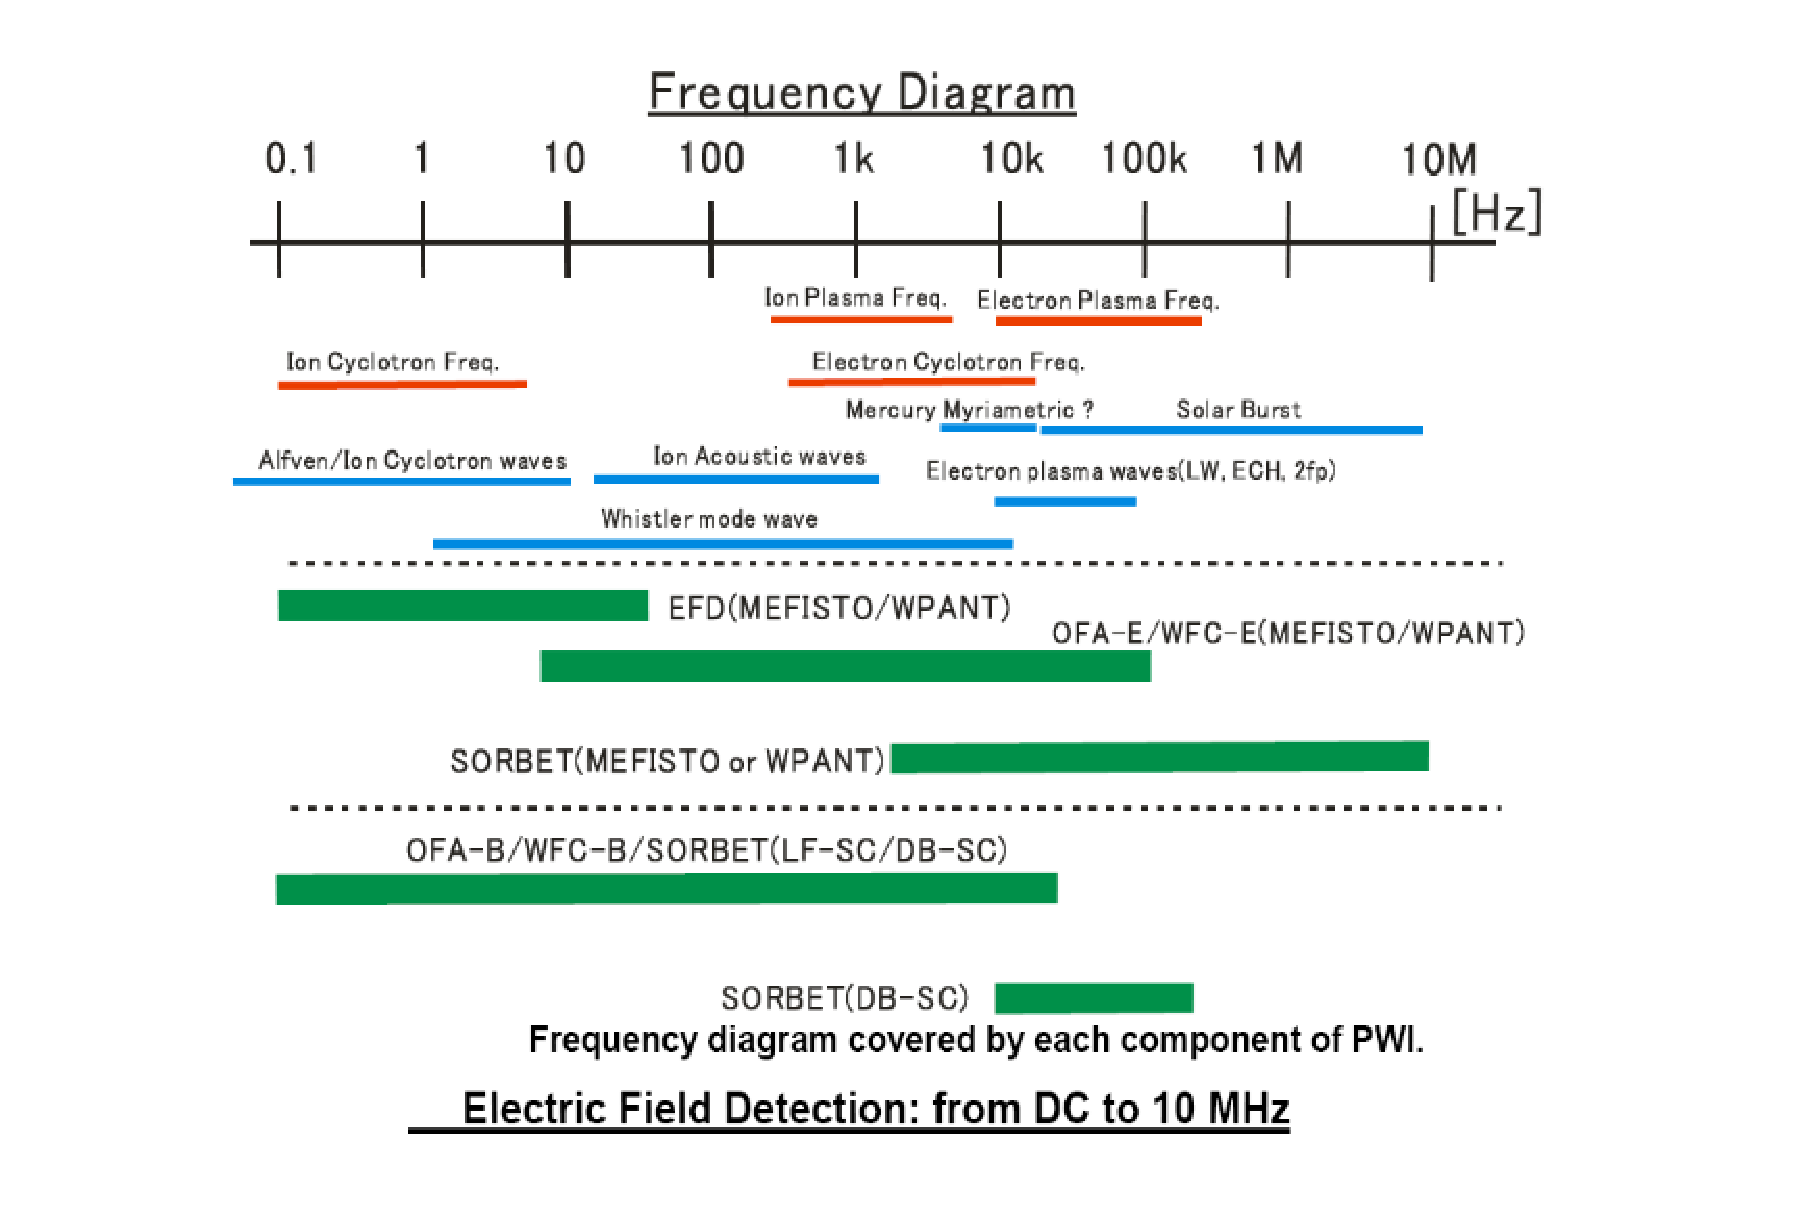
\includegraphics[width=12cm]{pics/freq_range_bepi.eps}\\
\caption{Frequency range of the expected plasma waves measured by Bepi Colombo}\label{fig_freq_range_bepi}
\end{figure}

\begin{figure}
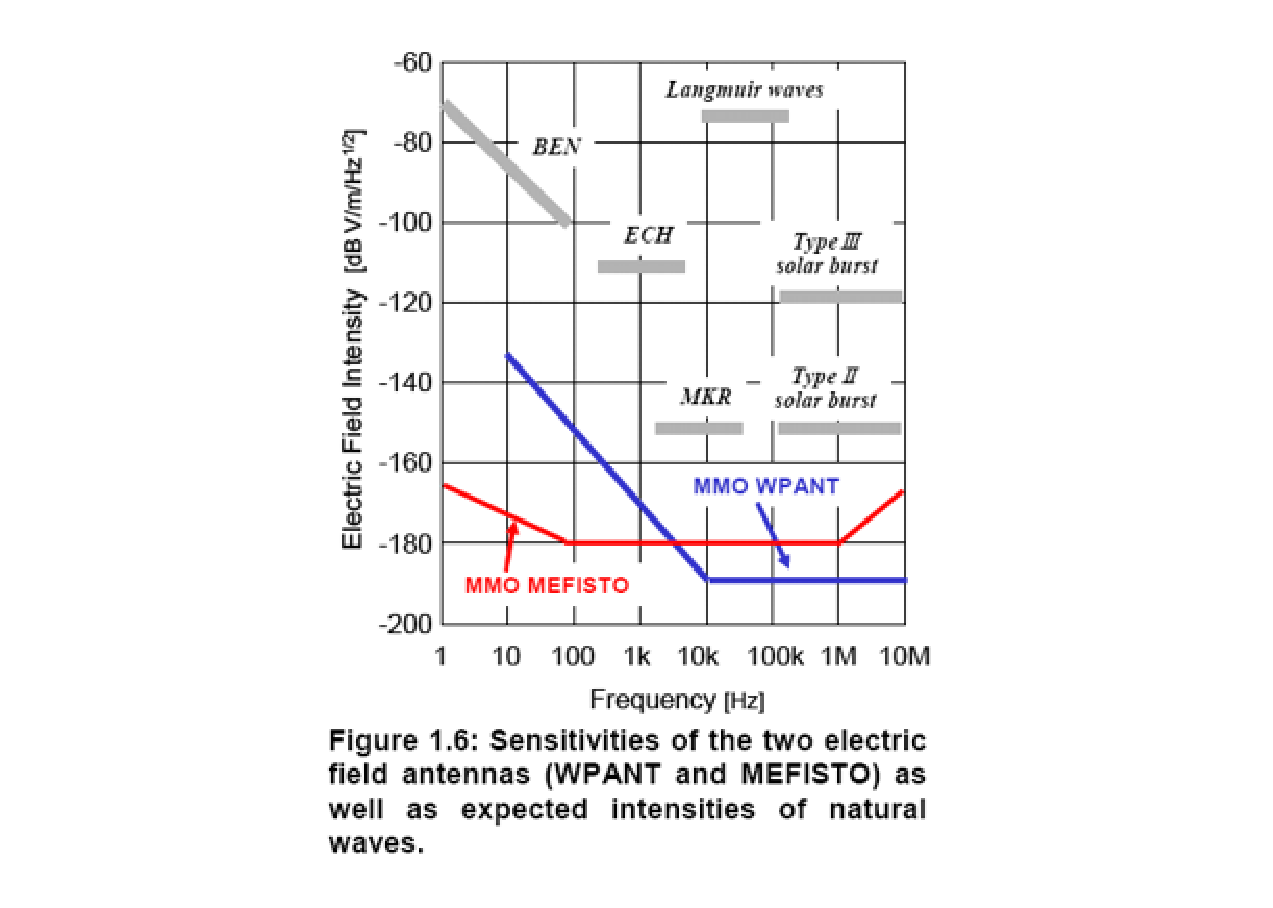
\includegraphics[width=12cm]{pics/bepi-sensitivity.eps}\\
\label{fig_sensi_bepi}
\end{figure}

\begin{figure}
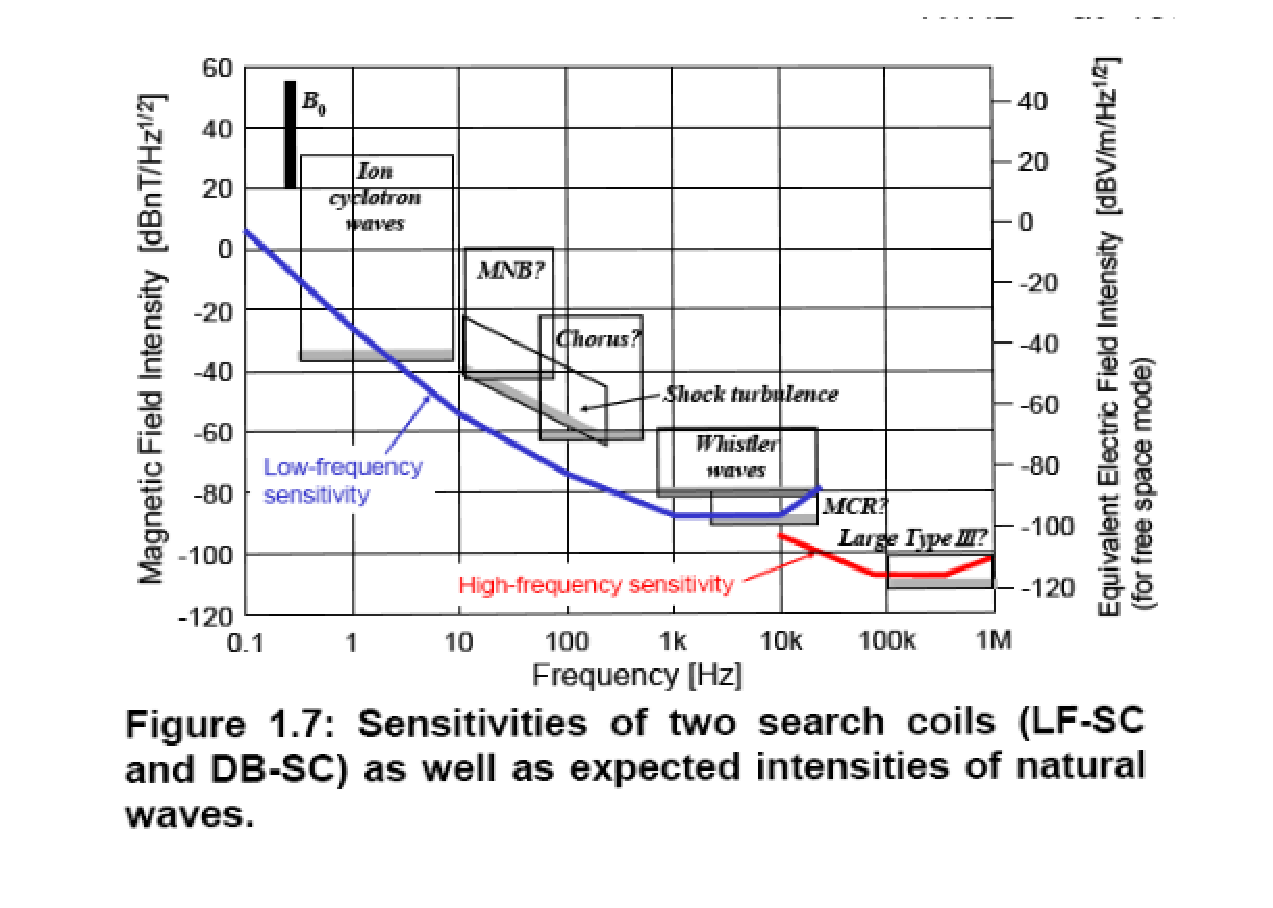
\includegraphics[width=12cm]{pics/sensi-mag.eps}\\
\label{fig_sensi_mag_bepi}
\end{figure}


The expected frequency ranges can be seen in figure \ref{fig_freq_range_bepi}.

\chapter{What to do}

\begin{itemize}
\item Effect of movement through the plasma
\item Effect of ion gap upon $I_{ph}$ and $I_e$
\item Effect of tunneling through ion gap
\item Effect of ion gap upon calculation of antenna impedance and effective height
\item Using the hot plasma tensor for calculation
\item Isolated part of the antennas taken into account ?
\item Is thermal noise routinely subtracted from radio observations ? see fig. \ref{fig_thermal_noise}
\item TNS: Effect of shotnoise on spheres
\item implement the MOM for antennas imbedded in plasma
\end{itemize}


\backmatter
\chapter{Appendix A}
\noindent\(\pmb{M=\{\{1,0,0\},\{0,1,0\},\{0,0,1\}\}}\\
\pmb{}\)

\noindent\(\{\{1,0,0\},\{0,1,0\},\{0,0,1\}\}\)

\noindent\(\pmb{\epsilon \epsilon =\epsilon _0\{\{S,-I*D,0\},\{I*D,S,0\},\{0,0,P\}\}}\)

\noindent\(\left\{\left\{S \epsilon _0,-i D \epsilon _0,0\right\},\left\{i D \epsilon _0,S \epsilon _0,0\right\},\left\{0,0,P \epsilon _0\right\}\right\}\)

\noindent\(\{\text{k1},\text{k2},\text{k3}\}\)

\noindent\(\pmb{}\\
\pmb{k=\{K*\text{Sin}[\alpha ]*\text{Cos}[\varphi ],K*\text{Sin}[\alpha ]*\text{Sin}[\varphi ],K*\text{Cos}[\alpha ]\}}\)

\noindent\(\{K \text{Cos}[\varphi ] \text{Sin}[\alpha ],K \text{Sin}[\alpha ] \text{Sin}[\varphi ],K \text{Cos}[\alpha ]\}\)

\noindent\(\pmb{\text{Outer}[\text{Times},k,k]}\)

\noindent\(\left\{\left\{\text{k1}^2,\text{k1} \text{k2},\text{k1} \text{k3}\right\},\left\{\text{k1} \text{k2},\text{k2}^2,\text{k2} \text{k3}\right\},\left\{\text{k1} \text{k3},\text{k2} \text{k3},\text{k3}^2\right\}\right\}\)

\noindent\(\left\{\left\{\text{k1}^2,\text{k1} \text{k2},\text{k1} \text{k3}\right\},\left\{\text{k1} \text{k2},\text{k2}^2,\text{k2} \text{k3}\right\},\left\{\text{k1} \text{k3},\text{k2} \text{k3},\text{k3}^2\right\}\right\}\)

\noindent\(\pmb{\lambda =k.k*M-\text{Outer}[\text{Times},k,k]-\mu _0*\omega {}^{\wedge}2*\epsilon \epsilon }\)

\noindent\(\left\{\left\{\text{k2}^2+\text{k3}^2-S \omega ^2 \epsilon _0 \mu _0,-\text{k1} \text{k2}+i D \omega ^2 \epsilon _0 \mu _0,-\text{k1} \text{k3}\right\},\right.\\
\left.\left\{-\text{k1} \text{k2}-i D \omega ^2 \epsilon _0 \mu _0,\text{k1}^2+\text{k3}^2-S \omega ^2 \epsilon _0 \mu _0,-\text{k2} \text{k3}\right\},\left\{-\text{k1} \text{k3},-\text{k2} \text{k3},\text{k1}^2+\text{k2}^2-P \omega ^2 \epsilon _0 \mu _0\right\}\right\}\)

\noindent\(\pmb{}\\
\pmb{\text{Simplify}[\lambda ]}\)

\noindent\(\left\{\left\{\text{k2}^2+\text{k3}^2-S \omega ^2 \epsilon _0 \mu _0,-\text{k1} \text{k2}+i D \omega ^2 \epsilon _0 \mu _0,-\text{k1} \text{k3}\right\},\right.\\
\left.\left\{-\text{k1} \text{k2}-i D \omega ^2 \epsilon _0 \mu _0,\text{k1}^2+\text{k3}^2-S \omega ^2 \epsilon _0 \mu _0,-\text{k2} \text{k3}\right\},\left\{-\text{k1} \text{k3},-\text{k2} \text{k3},\text{k1}^2+\text{k2}^2-P \omega ^2 \epsilon _0 \mu _0\right\}\right\}\)

\noindent\(\pmb{\text{detlam}=\text{Det}[\lambda ]}\)

\noindent\(-\text{k1}^2 \text{k3}^2 P \omega ^2 \epsilon _0 \mu _0-\text{k2}^2 \text{k3}^2 P \omega ^2 \epsilon _0 \mu _0-\text{k3}^4 P \omega ^2 \epsilon _0 \mu _0-\text{k1}^4 S \omega ^2 \epsilon _0 \mu _0-2 \text{k1}^2 \text{k2}^2 S \omega ^2 \epsilon _0 \mu _0-\\
\text{k2}^4 S \omega ^2 \epsilon _0 \mu _0-\text{k1}^2 \text{k3}^2 S \omega ^2 \epsilon _0 \mu _0-\text{k2}^2 \text{k3}^2 S \omega ^2 \epsilon _0 \mu _0-D^2 \text{k1}^2 \omega ^4 \epsilon _0^2 \mu _0^2-D^2 \text{k2}^2 \omega ^4 \epsilon _0^2 \mu _0^2+\text{k1}^2 P S \omega ^4 \epsilon _0^2 \mu _0^2+\\
\text{k2}^2 P S \omega ^4 \epsilon _0^2 \mu _0^2+2 \text{k3}^2 P S \omega ^4 \epsilon _0^2 \mu _0^2+\text{k1}^2 S^2 \omega ^4 \epsilon _0^2 \mu _0^2+\text{k2}^2 S^2 \omega ^4 \epsilon _0^2 \mu _0^2+D^2 P \omega ^6 \epsilon _0^3 \mu _0^3-P S^2 \omega ^6 \epsilon _0^3 \mu _0^3\)

\noindent\(\pmb{\text{Simplify}[\%]}\)

\noindent\(-\omega ^2 \epsilon _0 \mu _0 \left(\left(\text{k1}^2+\text{k2}^2+\text{k3}^2\right) \left(\text{k3}^2 P+\left(\text{k1}^2+\text{k2}^2\right) S\right)+\right.\\
\left.\left(D^2 \left(\text{k1}^2+\text{k2}^2\right)-S \left(2 \text{k3}^2 P+\text{k1}^2 (P+S)+\text{k2}^2 (P+S)\right)\right) \omega ^2 \epsilon _0 \mu _0+P \left(-D^2+S^2\right) \omega ^4 \epsilon _0^2 \mu _0^2\right)\)

\noindent\(\pmb{\text{FullSimplify}[\%]}\)

\noindent\(-\omega ^2 \epsilon _0 \mu _0 \left(\left(\text{k1}^2+\text{k2}^2+\text{k3}^2\right) \left(\text{k3}^2 P+\left(\text{k1}^2+\text{k2}^2\right) S\right)-\right.\\
\left.\omega ^2 \epsilon _0 \mu _0 \left(-D^2 \left(\text{k1}^2+\text{k2}^2\right)+S \left(2 \text{k3}^2 P+\text{k1}^2 (P+S)+\text{k2}^2 (P+S)\right)+P (D-S) (D+S) \omega ^2 \epsilon _0 \mu _0\right)\right)\)

\noindent\(\pmb{\%\text{/.}\text{k1}\to K*\text{Sin}[\alpha ]*\text{Cos}[\varphi ]}\)

\noindent\(-\omega ^2 \epsilon _0 \mu _0 \left(\left(\text{k2}^2+\text{k3}^2+K^2 \text{Cos}[\varphi ]^2 \text{Sin}[\alpha ]^2\right) \left(\text{k3}^2 P+S \left(\text{k2}^2+K^2 \text{Cos}[\varphi ]^2 \text{Sin}[\alpha ]^2\right)\right)-\right.\\
\omega ^2 \epsilon _0 \mu _0 \left(-D^2 \left(\text{k2}^2+K^2 \text{Cos}[\varphi ]^2 \text{Sin}[\alpha ]^2\right)+\right.\\
\left.\left.S \left(2 \text{k3}^2 P+\text{k2}^2 (P+S)+K^2 (P+S) \text{Cos}[\varphi ]^2 \text{Sin}[\alpha ]^2\right)+P (D-S) (D+S) \omega ^2 \epsilon _0 \mu _0\right)\right)\)

\noindent\(\pmb{}\\
\pmb{\%\text{/.}\text{k2}\to K*\text{Sin}[\alpha ]*\text{Sin}[\varphi ]}\)

\noindent\(-\omega ^2 \epsilon _0 \mu _0 \\
\left(\left(\text{k3}^2+K^2 \text{Cos}[\varphi ]^2 \text{Sin}[\alpha ]^2+K^2 \text{Sin}[\alpha ]^2 \text{Sin}[\varphi ]^2\right) \left(\text{k3}^2 P+S \left(K^2 \text{Cos}[\varphi ]^2 \text{Sin}[\alpha ]^2+K^2 \text{Sin}[\alpha ]^2 \text{Sin}[\varphi ]^2\right)\right)-\right.\\
\omega ^2 \epsilon _0 \mu _0 \left(-D^2 \left(K^2 \text{Cos}[\varphi ]^2 \text{Sin}[\alpha ]^2+K^2 \text{Sin}[\alpha ]^2 \text{Sin}[\varphi ]^2\right)+\right.\\
\left.\left.S \left(2 \text{k3}^2 P+K^2 (P+S) \text{Cos}[\varphi ]^2 \text{Sin}[\alpha ]^2+K^2 (P+S) \text{Sin}[\alpha ]^2 \text{Sin}[\varphi ]^2\right)+P (D-S) (D+S) \omega ^2 \epsilon _0 \mu _0\right)\right)\)

\noindent\(\pmb{\%\text{/.}\text{k3}\to K*\text{Cos}[\alpha ]}\\
\pmb{}\)

\noindent\(-\omega ^2 \epsilon _0 \mu _0 \left(\left(K^2 \text{Cos}[\alpha ]^2+K^2 \text{Cos}[\varphi ]^2 \text{Sin}[\alpha ]^2+K^2 \text{Sin}[\alpha ]^2 \text{Sin}[\varphi ]^2\right) \right.\\
\left(K^2 P \text{Cos}[\alpha ]^2+S \left(K^2 \text{Cos}[\varphi ]^2 \text{Sin}[\alpha ]^2+K^2 \text{Sin}[\alpha ]^2 \text{Sin}[\varphi ]^2\right)\right)-\\
\omega ^2 \epsilon _0 \mu _0 \left(-D^2 \left(K^2 \text{Cos}[\varphi ]^2 \text{Sin}[\alpha ]^2+K^2 \text{Sin}[\alpha ]^2 \text{Sin}[\varphi ]^2\right)+S \right.\\
\left.\left.\left(2 K^2 P \text{Cos}[\alpha ]^2+K^2 (P+S) \text{Cos}[\varphi ]^2 \text{Sin}[\alpha ]^2+K^2 (P+S) \text{Sin}[\alpha ]^2 \text{Sin}[\varphi ]^2\right)+P (D-S) (D+S) \omega ^2 \epsilon _0 \mu _0\right)\right)\)

\noindent\(\pmb{\text{Simplify}[\%]}\)

\noindent\(-\frac{1}{2} \omega ^2 \epsilon _0 \mu _0 \left(K^4 (P+S+(P-S) \text{Cos}[2 \alpha ])-\right.\\
\left.\omega ^2 \epsilon _0 \mu _0 \left(K^2 \left(-D^2+3 P S+S^2+\left(D^2+(P-S) S\right) \text{Cos}[2 \alpha ]\right)+2 P \left(D^2-S^2\right) \omega ^2 \epsilon _0 \mu _0\right)\right)\)

\noindent\(\pmb{\text{FullSimplify}[\%]}\\
\pmb{}\)

\noindent\(\frac{1}{2} \omega ^2 \epsilon _0 \mu _0 \left(-K^4 (P+S+(P-S) \text{Cos}[2 \alpha ])+\right.\\
\left.\omega ^2 \epsilon _0 \mu _0 \left(K^2 \left(-D^2+3 P S+S^2+\left(D^2+(P-S) S\right) \text{Cos}[2 \alpha ]\right)+2 P (D-S) (D+S) \omega ^2 \epsilon _0 \mu _0\right)\right)\)

\noindent\(\pmb{\text{Inverse}[\lambda ]}\)

\noindent\(\left\{\left\{\left.\left(-\text{k2}^2 \text{k3}^2+\left(\text{k1}^2+\text{k2}^2-P \omega ^2 \epsilon _0 \mu _0\right) \left(\text{k1}^2+\text{k3}^2-S \omega ^2 \epsilon _0 \mu _0\right)\right)\right/\right.\right.\\
\left(-\text{k1}^2 \text{k3}^2 P \omega ^2 \epsilon _0 \mu _0-\text{k2}^2 \text{k3}^2 P \omega ^2 \epsilon _0 \mu _0-\text{k3}^4 P \omega ^2 \epsilon _0 \mu _0-\text{k1}^4 S \omega ^2 \epsilon _0 \mu _0-2 \text{k1}^2 \text{k2}^2 S \omega ^2 \epsilon _0 \mu _0-\right.\\
\text{k2}^4 S \omega ^2 \epsilon _0 \mu _0-\text{k1}^2 \text{k3}^2 S \omega ^2 \epsilon _0 \mu _0-\text{k2}^2 \text{k3}^2 S \omega ^2 \epsilon _0 \mu _0-D^2 \text{k1}^2 \omega ^4 \epsilon _0^2 \mu _0^2-D^2 \text{k2}^2 \omega ^4 \epsilon _0^2 \mu _0^2+\text{k1}^2 P S \omega ^4 \epsilon _0^2 \mu _0^2+\\
\left.\text{k2}^2 P S \omega ^4 \epsilon _0^2 \mu _0^2+2 \text{k3}^2 P S \omega ^4 \epsilon _0^2 \mu _0^2+\text{k1}^2 S^2 \omega ^4 \epsilon _0^2 \mu _0^2+\text{k2}^2 S^2 \omega ^4 \epsilon _0^2 \mu _0^2+D^2 P \omega ^6 \epsilon _0^3 \mu _0^3-P S^2 \omega ^6 \epsilon _0^3 \mu _0^3\right),\\
\left.\left(\text{k1} \text{k2} \text{k3}^2-\left(-\text{k1} \text{k2}+i D \omega ^2 \epsilon _0 \mu _0\right) \left(\text{k1}^2+\text{k2}^2-P \omega ^2 \epsilon _0 \mu _0\right)\right)\right/\\
\left(-\text{k1}^2 \text{k3}^2 P \omega ^2 \epsilon _0 \mu _0-\text{k2}^2 \text{k3}^2 P \omega ^2 \epsilon _0 \mu _0-\text{k3}^4 P \omega ^2 \epsilon _0 \mu _0-\text{k1}^4 S \omega ^2 \epsilon _0 \mu _0-2 \text{k1}^2 \text{k2}^2 S \omega ^2 \epsilon _0 \mu _0-\right.\\
\text{k2}^4 S \omega ^2 \epsilon _0 \mu _0-\text{k1}^2 \text{k3}^2 S \omega ^2 \epsilon _0 \mu _0-\text{k2}^2 \text{k3}^2 S \omega ^2 \epsilon _0 \mu _0-D^2 \text{k1}^2 \omega ^4 \epsilon _0^2 \mu _0^2-D^2 \text{k2}^2 \omega ^4 \epsilon _0^2 \mu _0^2+\text{k1}^2 P S \omega ^4 \epsilon _0^2 \mu _0^2+\\
\left.\text{k2}^2 P S \omega ^4 \epsilon _0^2 \mu _0^2+2 \text{k3}^2 P S \omega ^4 \epsilon _0^2 \mu _0^2+\text{k1}^2 S^2 \omega ^4 \epsilon _0^2 \mu _0^2+\text{k2}^2 S^2 \omega ^4 \epsilon _0^2 \mu _0^2+D^2 P \omega ^6 \epsilon _0^3 \mu _0^3-P S^2 \omega ^6 \epsilon _0^3 \mu _0^3\right),\\
\left.\left(\text{k1}^3 \text{k3}+\text{k1} \text{k2}^2 \text{k3}+\text{k1} \text{k3}^3-i D \text{k2} \text{k3} \omega ^2 \epsilon _0 \mu _0-\text{k1} \text{k3} S \omega ^2 \epsilon _0 \mu _0\right)\right/\\
\left(-\text{k1}^2 \text{k3}^2 P \omega ^2 \epsilon _0 \mu _0-\text{k2}^2 \text{k3}^2 P \omega ^2 \epsilon _0 \mu _0-\text{k3}^4 P \omega ^2 \epsilon _0 \mu _0-\text{k1}^4 S \omega ^2 \epsilon _0 \mu _0-2 \text{k1}^2 \text{k2}^2 S \omega ^2 \epsilon _0 \mu _0-\right.\\
\text{k2}^4 S \omega ^2 \epsilon _0 \mu _0-\text{k1}^2 \text{k3}^2 S \omega ^2 \epsilon _0 \mu _0-\text{k2}^2 \text{k3}^2 S \omega ^2 \epsilon _0 \mu _0-D^2 \text{k1}^2 \omega ^4 \epsilon _0^2 \mu _0^2-D^2 \text{k2}^2 \omega ^4 \epsilon _0^2 \mu _0^2+\text{k1}^2 P S \omega ^4 \epsilon _0^2 \mu _0^2+\\
\left.\left.\text{k2}^2 P S \omega ^4 \epsilon _0^2 \mu _0^2+2 \text{k3}^2 P S \omega ^4 \epsilon _0^2 \mu _0^2+\text{k1}^2 S^2 \omega ^4 \epsilon _0^2 \mu _0^2+\text{k2}^2 S^2 \omega ^4 \epsilon _0^2 \mu _0^2+D^2 P \omega ^6 \epsilon _0^3 \mu _0^3-P S^2 \omega ^6 \epsilon _0^3 \mu _0^3\right)\right\},\\
\left\{\left.\left(\text{k1} \text{k2} \text{k3}^2-\left(-\text{k1} \text{k2}-i D \omega ^2 \epsilon _0 \mu _0\right) \left(\text{k1}^2+\text{k2}^2-P \omega ^2 \epsilon _0 \mu _0\right)\right)\right/\right.\\
\left(-\text{k1}^2 \text{k3}^2 P \omega ^2 \epsilon _0 \mu _0-\text{k2}^2 \text{k3}^2 P \omega ^2 \epsilon _0 \mu _0-\text{k3}^4 P \omega ^2 \epsilon _0 \mu _0-\text{k1}^4 S \omega ^2 \epsilon _0 \mu _0-2 \text{k1}^2 \text{k2}^2 S \omega ^2 \epsilon _0 \mu _0-\right.\\
\text{k2}^4 S \omega ^2 \epsilon _0 \mu _0-\text{k1}^2 \text{k3}^2 S \omega ^2 \epsilon _0 \mu _0-\text{k2}^2 \text{k3}^2 S \omega ^2 \epsilon _0 \mu _0-D^2 \text{k1}^2 \omega ^4 \epsilon _0^2 \mu _0^2-D^2 \text{k2}^2 \omega ^4 \epsilon _0^2 \mu _0^2+\text{k1}^2 P S \omega ^4 \epsilon _0^2 \mu _0^2+\\
\left.\text{k2}^2 P S \omega ^4 \epsilon _0^2 \mu _0^2+2 \text{k3}^2 P S \omega ^4 \epsilon _0^2 \mu _0^2+\text{k1}^2 S^2 \omega ^4 \epsilon _0^2 \mu _0^2+\text{k2}^2 S^2 \omega ^4 \epsilon _0^2 \mu _0^2+D^2 P \omega ^6 \epsilon _0^3 \mu _0^3-P S^2 \omega ^6 \epsilon _0^3 \mu _0^3\right),\\
\left.\left(-\text{k1}^2 \text{k3}^2+\left(\text{k1}^2+\text{k2}^2-P \omega ^2 \epsilon _0 \mu _0\right) \left(\text{k2}^2+\text{k3}^2-S \omega ^2 \epsilon _0 \mu _0\right)\right)\right/\\
\left(-\text{k1}^2 \text{k3}^2 P \omega ^2 \epsilon _0 \mu _0-\text{k2}^2 \text{k3}^2 P \omega ^2 \epsilon _0 \mu _0-\text{k3}^4 P \omega ^2 \epsilon _0 \mu _0-\text{k1}^4 S \omega ^2 \epsilon _0 \mu _0-2 \text{k1}^2 \text{k2}^2 S \omega ^2 \epsilon _0 \mu _0-\right.\\
\text{k2}^4 S \omega ^2 \epsilon _0 \mu _0-\text{k1}^2 \text{k3}^2 S \omega ^2 \epsilon _0 \mu _0-\text{k2}^2 \text{k3}^2 S \omega ^2 \epsilon _0 \mu _0-D^2 \text{k1}^2 \omega ^4 \epsilon _0^2 \mu _0^2-D^2 \text{k2}^2 \omega ^4 \epsilon _0^2 \mu _0^2+\text{k1}^2 P S \omega ^4 \epsilon _0^2 \mu _0^2+\\
\left.\text{k2}^2 P S \omega ^4 \epsilon _0^2 \mu _0^2+2 \text{k3}^2 P S \omega ^4 \epsilon _0^2 \mu _0^2+\text{k1}^2 S^2 \omega ^4 \epsilon _0^2 \mu _0^2+\text{k2}^2 S^2 \omega ^4 \epsilon _0^2 \mu _0^2+D^2 P \omega ^6 \epsilon _0^3 \mu _0^3-P S^2 \omega ^6 \epsilon _0^3 \mu _0^3\right),\\
\left.\left(\text{k1}^2 \text{k2} \text{k3}+\text{k2}^3 \text{k3}+\text{k2} \text{k3}^3+i D \text{k1} \text{k3} \omega ^2 \epsilon _0 \mu _0-\text{k2} \text{k3} S \omega ^2 \epsilon _0 \mu _0\right)\right/\\
\left(-\text{k1}^2 \text{k3}^2 P \omega ^2 \epsilon _0 \mu _0-\text{k2}^2 \text{k3}^2 P \omega ^2 \epsilon _0 \mu _0-\text{k3}^4 P \omega ^2 \epsilon _0 \mu _0-\text{k1}^4 S \omega ^2 \epsilon _0 \mu _0-2 \text{k1}^2 \text{k2}^2 S \omega ^2 \epsilon _0 \mu _0-\right.\\
\text{k2}^4 S \omega ^2 \epsilon _0 \mu _0-\text{k1}^2 \text{k3}^2 S \omega ^2 \epsilon _0 \mu _0-\text{k2}^2 \text{k3}^2 S \omega ^2 \epsilon _0 \mu _0-D^2 \text{k1}^2 \omega ^4 \epsilon _0^2 \mu _0^2-D^2 \text{k2}^2 \omega ^4 \epsilon _0^2 \mu _0^2+\text{k1}^2 P S \omega ^4 \epsilon _0^2 \mu _0^2+\\
\left.\left.\text{k2}^2 P S \omega ^4 \epsilon _0^2 \mu _0^2+2 \text{k3}^2 P S \omega ^4 \epsilon _0^2 \mu _0^2+\text{k1}^2 S^2 \omega ^4 \epsilon _0^2 \mu _0^2+\text{k2}^2 S^2 \omega ^4 \epsilon _0^2 \mu _0^2+D^2 P \omega ^6 \epsilon _0^3 \mu _0^3-P S^2 \omega ^6 \epsilon _0^3 \mu _0^3\right)\right\},\\
\left\{\left.\left(\text{k1}^3 \text{k3}+\text{k1} \text{k2}^2 \text{k3}+\text{k1} \text{k3}^3+i D \text{k2} \text{k3} \omega ^2 \epsilon _0 \mu _0-\text{k1} \text{k3} S \omega ^2 \epsilon _0 \mu _0\right)\right/\right.\\
\left(-\text{k1}^2 \text{k3}^2 P \omega ^2 \epsilon _0 \mu _0-\text{k2}^2 \text{k3}^2 P \omega ^2 \epsilon _0 \mu _0-\text{k3}^4 P \omega ^2 \epsilon _0 \mu _0-\text{k1}^4 S \omega ^2 \epsilon _0 \mu _0-2 \text{k1}^2 \text{k2}^2 S \omega ^2 \epsilon _0 \mu _0-\right.\\
\text{k2}^4 S \omega ^2 \epsilon _0 \mu _0-\text{k1}^2 \text{k3}^2 S \omega ^2 \epsilon _0 \mu _0-\text{k2}^2 \text{k3}^2 S \omega ^2 \epsilon _0 \mu _0-D^2 \text{k1}^2 \omega ^4 \epsilon _0^2 \mu _0^2-D^2 \text{k2}^2 \omega ^4 \epsilon _0^2 \mu _0^2+\text{k1}^2 P S \omega ^4 \epsilon _0^2 \mu _0^2+\\
\left.\text{k2}^2 P S \omega ^4 \epsilon _0^2 \mu _0^2+2 \text{k3}^2 P S \omega ^4 \epsilon _0^2 \mu _0^2+\text{k1}^2 S^2 \omega ^4 \epsilon _0^2 \mu _0^2+\text{k2}^2 S^2 \omega ^4 \epsilon _0^2 \mu _0^2+D^2 P \omega ^6 \epsilon _0^3 \mu _0^3-P S^2 \omega ^6 \epsilon _0^3 \mu _0^3\right),\\
\left.\left(\text{k1}^2 \text{k2} \text{k3}+\text{k2}^3 \text{k3}+\text{k2} \text{k3}^3-i D \text{k1} \text{k3} \omega ^2 \epsilon _0 \mu _0-\text{k2} \text{k3} S \omega ^2 \epsilon _0 \mu _0\right)\right/\\
\left(-\text{k1}^2 \text{k3}^2 P \omega ^2 \epsilon _0 \mu _0-\text{k2}^2 \text{k3}^2 P \omega ^2 \epsilon _0 \mu _0-\text{k3}^4 P \omega ^2 \epsilon _0 \mu _0-\text{k1}^4 S \omega ^2 \epsilon _0 \mu _0-2 \text{k1}^2 \text{k2}^2 S \omega ^2 \epsilon _0 \mu _0-\right.\\
\text{k2}^4 S \omega ^2 \epsilon _0 \mu _0-\text{k1}^2 \text{k3}^2 S \omega ^2 \epsilon _0 \mu _0-\text{k2}^2 \text{k3}^2 S \omega ^2 \epsilon _0 \mu _0-D^2 \text{k1}^2 \omega ^4 \epsilon _0^2 \mu _0^2-D^2 \text{k2}^2 \omega ^4 \epsilon _0^2 \mu _0^2+\text{k1}^2 P S \omega ^4 \epsilon _0^2 \mu _0^2+\\
\left.\text{k2}^2 P S \omega ^4 \epsilon _0^2 \mu _0^2+2 \text{k3}^2 P S \omega ^4 \epsilon _0^2 \mu _0^2+\text{k1}^2 S^2 \omega ^4 \epsilon _0^2 \mu _0^2+\text{k2}^2 S^2 \omega ^4 \epsilon _0^2 \mu _0^2+D^2 P \omega ^6 \epsilon _0^3 \mu _0^3-P S^2 \omega ^6 \epsilon _0^3 \mu _0^3\right),\\
\left.\left(\text{k1}^2 \text{k3}^2+\text{k2}^2 \text{k3}^2+\text{k3}^4-\text{k1}^2 S \omega ^2 \epsilon _0 \mu _0-\text{k2}^2 S \omega ^2 \epsilon _0 \mu _0-2 \text{k3}^2 S \omega ^2 \epsilon _0 \mu _0-D^2 \omega ^4 \epsilon _0^2 \mu _0^2+S^2 \omega ^4 \epsilon _0^2 \mu _0^2\right)\right/\\
\left(-\text{k1}^2 \text{k3}^2 P \omega ^2 \epsilon _0 \mu _0-\text{k2}^2 \text{k3}^2 P \omega ^2 \epsilon _0 \mu _0-\text{k3}^4 P \omega ^2 \epsilon _0 \mu _0-\text{k1}^4 S \omega ^2 \epsilon _0 \mu _0-2 \text{k1}^2 \text{k2}^2 S \omega ^2 \epsilon _0 \mu _0-\right.\\
\text{k2}^4 S \omega ^2 \epsilon _0 \mu _0-\text{k1}^2 \text{k3}^2 S \omega ^2 \epsilon _0 \mu _0-\text{k2}^2 \text{k3}^2 S \omega ^2 \epsilon _0 \mu _0-D^2 \text{k1}^2 \omega ^4 \epsilon _0^2 \mu _0^2-D^2 \text{k2}^2 \omega ^4 \epsilon _0^2 \mu _0^2+\text{k1}^2 P S \omega ^4 \epsilon _0^2 \mu _0^2+\\
\left.\left.\left.\text{k2}^2 P S \omega ^4 \epsilon _0^2 \mu _0^2+2 \text{k3}^2 P S \omega ^4 \epsilon _0^2 \mu _0^2+\text{k1}^2 S^2 \omega ^4 \epsilon _0^2 \mu _0^2+\text{k2}^2 S^2 \omega ^4 \epsilon _0^2 \mu _0^2+D^2 P \omega ^6 \epsilon _0^3 \mu _0^3-P S^2 \omega ^6 \epsilon _0^3 \mu _0^3\right)\right\}\right\}\)

\noindent\(\pmb{\text{FullSimplify}[\%]}\)

\noindent\(\left\{\left\{\left.\left(-\text{k1}^2 \left(\text{k1}^2+\text{k2}^2+\text{k3}^2\right)+\omega ^2 \epsilon _0 \mu _0 \left(\text{k3}^2 P+\text{k2}^2 S+\text{k1}^2 (P+S)-P S \omega ^2 \epsilon _0 \mu _0\right)\right)\right/\right.\right.\\
\left(\omega ^2 \epsilon _0 \mu _0 \left(\left(\text{k1}^2+\text{k2}^2+\text{k3}^2\right) \left(\text{k3}^2 P+\left(\text{k1}^2+\text{k2}^2\right) S\right)-\right.\right.\\
\left.\left.\omega ^2 \epsilon _0 \mu _0 \left(-D^2 \left(\text{k1}^2+\text{k2}^2\right)+S \left(2 \text{k3}^2 P+\text{k1}^2 (P+S)+\text{k2}^2 (P+S)\right)+P (D-S) (D+S) \omega ^2 \epsilon _0 \mu _0\right)\right)\right),\\
\left.\left(-\text{k1} \text{k2} \left(\text{k1}^2+\text{k2}^2+\text{k3}^2\right)+\omega ^2 \epsilon _0 \mu _0 \left(i D \left(\text{k1}^2+\text{k2}^2\right)+\text{k1} \text{k2} P-i D P \omega ^2 \epsilon _0 \mu _0\right)\right)\right/\\
\left(\omega ^2 \epsilon _0 \mu _0 \left(\left(\text{k1}^2+\text{k2}^2+\text{k3}^2\right) \left(\text{k3}^2 P+\left(\text{k1}^2+\text{k2}^2\right) S\right)-\right.\right.\\
\left.\left.\omega ^2 \epsilon _0 \mu _0 \left(-D^2 \left(\text{k1}^2+\text{k2}^2\right)+S \left(2 \text{k3}^2 P+\text{k1}^2 (P+S)+\text{k2}^2 (P+S)\right)+P (D-S) (D+S) \omega ^2 \epsilon _0 \mu _0\right)\right)\right),\\
\left(-\text{k1} \text{k3} \left(\text{k1}^2+\text{k2}^2+\text{k3}^2\right)+\text{k3} (i D \text{k2}+\text{k1} S) \omega ^2 \epsilon _0 \mu _0\right)/\left(\omega ^2 \epsilon _0 \mu _0 \left(\left(\text{k1}^2+\text{k2}^2+\text{k3}^2\right) \left(\text{k3}^2 P+\left(\text{k1}^2+\text{k2}^2\right) S\right)-\right.\right.\\
\left.\left.\left.\omega ^2 \epsilon _0 \mu _0 \left(-D^2 \left(\text{k1}^2+\text{k2}^2\right)+S \left(2 \text{k3}^2 P+\text{k1}^2 (P+S)+\text{k2}^2 (P+S)\right)+P (D-S) (D+S) \omega ^2 \epsilon _0 \mu _0\right)\right)\right)\right\},\\
\left\{-\left.\left(\text{k1} \text{k2} \left(\text{k1}^2+\text{k2}^2+\text{k3}^2\right)+i \omega ^2 \epsilon _0 \mu _0 \left(D \left(\text{k1}^2+\text{k2}^2\right)+i \text{k1} \text{k2} P-D P \omega ^2 \epsilon _0 \mu _0\right)\right)\right/\right.\\
\left(\omega ^2 \epsilon _0 \mu _0 \left(\left(\text{k1}^2+\text{k2}^2+\text{k3}^2\right) \left(\text{k3}^2 P+\left(\text{k1}^2+\text{k2}^2\right) S\right)-\right.\right.\\
\left.\left.\omega ^2 \epsilon _0 \mu _0 \left(-D^2 \left(\text{k1}^2+\text{k2}^2\right)+S \left(2 \text{k3}^2 P+\text{k1}^2 (P+S)+\text{k2}^2 (P+S)\right)+P (D-S) (D+S) \omega ^2 \epsilon _0 \mu _0\right)\right)\right),\\
\left.\left(-\text{k2}^2 \left(\text{k1}^2+\text{k2}^2+\text{k3}^2\right)+\omega ^2 \epsilon _0 \mu _0 \left(\text{k3}^2 P+\text{k1}^2 S+\text{k2}^2 (P+S)-P S \omega ^2 \epsilon _0 \mu _0\right)\right)\right/\\
\left(\omega ^2 \epsilon _0 \mu _0 \left(\left(\text{k1}^2+\text{k2}^2+\text{k3}^2\right) \left(\text{k3}^2 P+\left(\text{k1}^2+\text{k2}^2\right) S\right)-\right.\right.\\
\left.\left.\omega ^2 \epsilon _0 \mu _0 \left(-D^2 \left(\text{k1}^2+\text{k2}^2\right)+S \left(2 \text{k3}^2 P+\text{k1}^2 (P+S)+\text{k2}^2 (P+S)\right)+P (D-S) (D+S) \omega ^2 \epsilon _0 \mu _0\right)\right)\right),\\
\left(-\text{k2} \text{k3} \left(\text{k1}^2+\text{k2}^2+\text{k3}^2\right)+\text{k3} (-i D \text{k1}+\text{k2} S) \omega ^2 \epsilon _0 \mu _0\right)/\left(\omega ^2 \epsilon _0 \mu _0 \left(\left(\text{k1}^2+\text{k2}^2+\text{k3}^2\right) \left(\text{k3}^2 P+\left(\text{k1}^2+\text{k2}^2\right) S\right)-\right.\right.\\
\left.\left.\left.\omega ^2 \epsilon _0 \mu _0 \left(-D^2 \left(\text{k1}^2+\text{k2}^2\right)+S \left(2 \text{k3}^2 P+\text{k1}^2 (P+S)+\text{k2}^2 (P+S)\right)+P (D-S) (D+S) \omega ^2 \epsilon _0 \mu _0\right)\right)\right)\right\},\\
\left\{\left(-\text{k1} \text{k3} \left(\text{k1}^2+\text{k2}^2+\text{k3}^2\right)+\text{k3} (-i D \text{k2}+\text{k1} S) \omega ^2 \epsilon _0 \mu _0\right)/\left(\omega ^2 \epsilon _0 \mu _0 \left(\left(\text{k1}^2+\text{k2}^2+\text{k3}^2\right) \left(\text{k3}^2 P+\left(\text{k1}^2+\text{k2}^2\right) S\right)-\right.\right.\right.\\
\left.\left.\omega ^2 \epsilon _0 \mu _0 \left(-D^2 \left(\text{k1}^2+\text{k2}^2\right)+S \left(2 \text{k3}^2 P+\text{k1}^2 (P+S)+\text{k2}^2 (P+S)\right)+P (D-S) (D+S) \omega ^2 \epsilon _0 \mu _0\right)\right)\right),\\
\left(-\text{k2} \text{k3} \left(\text{k1}^2+\text{k2}^2+\text{k3}^2\right)+\text{k3} (i D \text{k1}+\text{k2} S) \omega ^2 \epsilon _0 \mu _0\right)/\left(\omega ^2 \epsilon _0 \mu _0 \left(\left(\text{k1}^2+\text{k2}^2+\text{k3}^2\right) \left(\text{k3}^2 P+\left(\text{k1}^2+\text{k2}^2\right) S\right)-\right.\right.\\
\left.\left.\omega ^2 \epsilon _0 \mu _0 \left(-D^2 \left(\text{k1}^2+\text{k2}^2\right)+S \left(2 \text{k3}^2 P+\text{k1}^2 (P+S)+\text{k2}^2 (P+S)\right)+P (D-S) (D+S) \omega ^2 \epsilon _0 \mu _0\right)\right)\right),\\
\left.\left(-\text{k3}^2 \left(\text{k1}^2+\text{k2}^2+\text{k3}^2\right)+\omega ^2 \epsilon _0 \mu _0 \left(\left(\text{k1}^2+\text{k2}^2+2 \text{k3}^2\right) S+(D-S) (D+S) \omega ^2 \epsilon _0 \mu _0\right)\right)\right/\\
\left(\omega ^2 \epsilon _0 \mu _0 \left(\left(\text{k1}^2+\text{k2}^2+\text{k3}^2\right) \left(\text{k3}^2 P+\left(\text{k1}^2+\text{k2}^2\right) S\right)-\right.\right.\\
\left.\left.\left.\left.\omega ^2 \epsilon _0 \mu _0 \left(-D^2 \left(\text{k1}^2+\text{k2}^2\right)+S \left(2 \text{k3}^2 P+\text{k1}^2 (P+S)+\text{k2}^2 (P+S)\right)+P (D-S) (D+S) \omega ^2 \epsilon _0 \mu _0\right)\right)\right)\right\}\right\}\)

\noindent\(\pmb{\%\text{/.}\text{k1}\to K*\text{Sin}[\alpha ]*\text{Cos}[\varphi ]}\)

\noindent\(\left\{\left\{\left(-K^2 \text{Cos}[\varphi ]^2 \text{Sin}[\alpha ]^2 \left(\text{k2}^2+\text{k3}^2+K^2 \text{Cos}[\varphi ]^2 \text{Sin}[\alpha ]^2\right)+\right.\right.\right.\\
\left.\left.\omega ^2 \epsilon _0 \mu _0 \left(\text{k3}^2 P+\text{k2}^2 S+K^2 (P+S) \text{Cos}[\varphi ]^2 \text{Sin}[\alpha ]^2-P S \omega ^2 \epsilon _0 \mu _0\right)\right)\right/\\
\left(\omega ^2 \epsilon _0 \mu _0 \left(\left(\text{k2}^2+\text{k3}^2+K^2 \text{Cos}[\varphi ]^2 \text{Sin}[\alpha ]^2\right) \left(\text{k3}^2 P+S \left(\text{k2}^2+K^2 \text{Cos}[\varphi ]^2 \text{Sin}[\alpha ]^2\right)\right)-\right.\right.\\
\omega ^2 \epsilon _0 \mu _0 \left(-D^2 \left(\text{k2}^2+K^2 \text{Cos}[\varphi ]^2 \text{Sin}[\alpha ]^2\right)+S \left(2 \text{k3}^2 P+\text{k2}^2 (P+S)+K^2 (P+S) \text{Cos}[\varphi ]^2 \text{Sin}[\alpha ]^2\right)+\right.\\
\left.\left.\left.P (D-S) (D+S) \omega ^2 \epsilon _0 \mu _0\right)\right)\right),\left(-K \text{k2} \text{Cos}[\varphi ] \text{Sin}[\alpha ] \left(\text{k2}^2+\text{k3}^2+K^2 \text{Cos}[\varphi ]^2 \text{Sin}[\alpha ]^2\right)+\right.\\
\left.\left.\omega ^2 \epsilon _0 \mu _0 \left(K \text{k2} P \text{Cos}[\varphi ] \text{Sin}[\alpha ]+i D \left(\text{k2}^2+K^2 \text{Cos}[\varphi ]^2 \text{Sin}[\alpha ]^2\right)-i D P \omega ^2 \epsilon _0 \mu _0\right)\right)\right/\\
\left(\omega ^2 \epsilon _0 \mu _0 \left(\left(\text{k2}^2+\text{k3}^2+K^2 \text{Cos}[\varphi ]^2 \text{Sin}[\alpha ]^2\right) \left(\text{k3}^2 P+S \left(\text{k2}^2+K^2 \text{Cos}[\varphi ]^2 \text{Sin}[\alpha ]^2\right)\right)-\right.\right.\\
\omega ^2 \epsilon _0 \mu _0 \left(-D^2 \left(\text{k2}^2+K^2 \text{Cos}[\varphi ]^2 \text{Sin}[\alpha ]^2\right)+\right.\\
\left.\left.\left.S \left(2 \text{k3}^2 P+\text{k2}^2 (P+S)+K^2 (P+S) \text{Cos}[\varphi ]^2 \text{Sin}[\alpha ]^2\right)+P (D-S) (D+S) \omega ^2 \epsilon _0 \mu _0\right)\right)\right),\\
\left.\left(-K \text{k3} \text{Cos}[\varphi ] \text{Sin}[\alpha ] \left(\text{k2}^2+\text{k3}^2+K^2 \text{Cos}[\varphi ]^2 \text{Sin}[\alpha ]^2\right)+\text{k3} \omega ^2 (i D \text{k2}+K S \text{Cos}[\varphi ] \text{Sin}[\alpha ]) \epsilon _0 \mu _0\right)\right/\\
\left(\omega ^2 \epsilon _0 \mu _0 \left(\left(\text{k2}^2+\text{k3}^2+K^2 \text{Cos}[\varphi ]^2 \text{Sin}[\alpha ]^2\right) \left(\text{k3}^2 P+S \left(\text{k2}^2+K^2 \text{Cos}[\varphi ]^2 \text{Sin}[\alpha ]^2\right)\right)-\right.\right.\\
\omega ^2 \epsilon _0 \mu _0 \left(-D^2 \left(\text{k2}^2+K^2 \text{Cos}[\varphi ]^2 \text{Sin}[\alpha ]^2\right)+\right.\\
\left.\left.\left.\left.S \left(2 \text{k3}^2 P+\text{k2}^2 (P+S)+K^2 (P+S) \text{Cos}[\varphi ]^2 \text{Sin}[\alpha ]^2\right)+P (D-S) (D+S) \omega ^2 \epsilon _0 \mu _0\right)\right)\right)\right\},\\
\left\{-\left(K \text{k2} \text{Cos}[\varphi ] \text{Sin}[\alpha ] \left(\text{k2}^2+\text{k3}^2+K^2 \text{Cos}[\varphi ]^2 \text{Sin}[\alpha ]^2\right)+i \omega ^2 \epsilon _0 \mu _0 \right.\right.\\
\left.\left.\left(i K \text{k2} P \text{Cos}[\varphi ] \text{Sin}[\alpha ]+D \left(\text{k2}^2+K^2 \text{Cos}[\varphi ]^2 \text{Sin}[\alpha ]^2\right)-D P \omega ^2 \epsilon _0 \mu _0\right)\right)\right/\\
\left(\omega ^2 \epsilon _0 \mu _0 \left(\left(\text{k2}^2+\text{k3}^2+K^2 \text{Cos}[\varphi ]^2 \text{Sin}[\alpha ]^2\right) \left(\text{k3}^2 P+S \left(\text{k2}^2+K^2 \text{Cos}[\varphi ]^2 \text{Sin}[\alpha ]^2\right)\right)-\right.\right.\\
\omega ^2 \epsilon _0 \mu _0 \left(-D^2 \left(\text{k2}^2+K^2 \text{Cos}[\varphi ]^2 \text{Sin}[\alpha ]^2\right)+\right.\\
\left.\left.\left.S \left(2 \text{k3}^2 P+\text{k2}^2 (P+S)+K^2 (P+S) \text{Cos}[\varphi ]^2 \text{Sin}[\alpha ]^2\right)+P (D-S) (D+S) \omega ^2 \epsilon _0 \mu _0\right)\right)\right),\\
\left.\left(-\text{k2}^2 \left(\text{k2}^2+\text{k3}^2+K^2 \text{Cos}[\varphi ]^2 \text{Sin}[\alpha ]^2\right)+\omega ^2 \epsilon _0 \mu _0 \left(\text{k3}^2 P+\text{k2}^2 (P+S)+K^2 S \text{Cos}[\varphi ]^2 \text{Sin}[\alpha ]^2-P S \omega ^2 \epsilon _0 \mu _0\right)\right)\right/\\
\left(\omega ^2 \epsilon _0 \mu _0 \left(\left(\text{k2}^2+\text{k3}^2+K^2 \text{Cos}[\varphi ]^2 \text{Sin}[\alpha ]^2\right) \left(\text{k3}^2 P+S \left(\text{k2}^2+K^2 \text{Cos}[\varphi ]^2 \text{Sin}[\alpha ]^2\right)\right)-\right.\right.\\
\omega ^2 \epsilon _0 \mu _0 \left(-D^2 \left(\text{k2}^2+K^2 \text{Cos}[\varphi ]^2 \text{Sin}[\alpha ]^2\right)+\right.\\
\left.\left.\left.S \left(2 \text{k3}^2 P+\text{k2}^2 (P+S)+K^2 (P+S) \text{Cos}[\varphi ]^2 \text{Sin}[\alpha ]^2\right)+P (D-S) (D+S) \omega ^2 \epsilon _0 \mu _0\right)\right)\right),\\
\left.\left(-\text{k2} \text{k3} \left(\text{k2}^2+\text{k3}^2+K^2 \text{Cos}[\varphi ]^2 \text{Sin}[\alpha ]^2\right)+\text{k3} \omega ^2 (\text{k2} S-i D K \text{Cos}[\varphi ] \text{Sin}[\alpha ]) \epsilon _0 \mu _0\right)\right/\\
\left(\omega ^2 \epsilon _0 \mu _0 \left(\left(\text{k2}^2+\text{k3}^2+K^2 \text{Cos}[\varphi ]^2 \text{Sin}[\alpha ]^2\right) \left(\text{k3}^2 P+S \left(\text{k2}^2+K^2 \text{Cos}[\varphi ]^2 \text{Sin}[\alpha ]^2\right)\right)-\right.\right.\\
\omega ^2 \epsilon _0 \mu _0 \left(-D^2 \left(\text{k2}^2+K^2 \text{Cos}[\varphi ]^2 \text{Sin}[\alpha ]^2\right)+\right.\\
\left.\left.\left.\left.S \left(2 \text{k3}^2 P+\text{k2}^2 (P+S)+K^2 (P+S) \text{Cos}[\varphi ]^2 \text{Sin}[\alpha ]^2\right)+P (D-S) (D+S) \omega ^2 \epsilon _0 \mu _0\right)\right)\right)\right\},\\
\left\{\left.\left(-K \text{k3} \text{Cos}[\varphi ] \text{Sin}[\alpha ] \left(\text{k2}^2+\text{k3}^2+K^2 \text{Cos}[\varphi ]^2 \text{Sin}[\alpha ]^2\right)+\text{k3} \omega ^2 (-i D \text{k2}+K S \text{Cos}[\varphi ] \text{Sin}[\alpha ]) \epsilon _0 \mu _0\right)\right/\right.\\
\left(\omega ^2 \epsilon _0 \mu _0 \left(\left(\text{k2}^2+\text{k3}^2+K^2 \text{Cos}[\varphi ]^2 \text{Sin}[\alpha ]^2\right) \left(\text{k3}^2 P+S \left(\text{k2}^2+K^2 \text{Cos}[\varphi ]^2 \text{Sin}[\alpha ]^2\right)\right)-\right.\right.\\
\omega ^2 \epsilon _0 \mu _0 \left(-D^2 \left(\text{k2}^2+K^2 \text{Cos}[\varphi ]^2 \text{Sin}[\alpha ]^2\right)+\right.\\
\left.\left.\left.S \left(2 \text{k3}^2 P+\text{k2}^2 (P+S)+K^2 (P+S) \text{Cos}[\varphi ]^2 \text{Sin}[\alpha ]^2\right)+P (D-S) (D+S) \omega ^2 \epsilon _0 \mu _0\right)\right)\right),\\
\left.\left(-\text{k2} \text{k3} \left(\text{k2}^2+\text{k3}^2+K^2 \text{Cos}[\varphi ]^2 \text{Sin}[\alpha ]^2\right)+\text{k3} \omega ^2 (\text{k2} S+i D K \text{Cos}[\varphi ] \text{Sin}[\alpha ]) \epsilon _0 \mu _0\right)\right/\\
\left(\omega ^2 \epsilon _0 \mu _0 \left(\left(\text{k2}^2+\text{k3}^2+K^2 \text{Cos}[\varphi ]^2 \text{Sin}[\alpha ]^2\right) \left(\text{k3}^2 P+S \left(\text{k2}^2+K^2 \text{Cos}[\varphi ]^2 \text{Sin}[\alpha ]^2\right)\right)-\right.\right.\\
\omega ^2 \epsilon _0 \mu _0 \left(-D^2 \left(\text{k2}^2+K^2 \text{Cos}[\varphi ]^2 \text{Sin}[\alpha ]^2\right)+S \left(2 \text{k3}^2 P+\text{k2}^2 (P+S)+K^2 (P+S) \text{Cos}[\varphi ]^2 \text{Sin}[\alpha ]^2\right)+\right.\\
\left.\left.\left.P (D-S) (D+S) \omega ^2 \epsilon _0 \mu _0\right)\right)\right),\left(-\text{k3}^2 \left(\text{k2}^2+\text{k3}^2+K^2 \text{Cos}[\varphi ]^2 \text{Sin}[\alpha ]^2\right)+\right.\\
\left.\left.\omega ^2 \epsilon _0 \mu _0 \left(S \left(\text{k2}^2+2 \text{k3}^2+K^2 \text{Cos}[\varphi ]^2 \text{Sin}[\alpha ]^2\right)+(D-S) (D+S) \omega ^2 \epsilon _0 \mu _0\right)\right)\right/\\
\left(\omega ^2 \epsilon _0 \mu _0 \left(\left(\text{k2}^2+\text{k3}^2+K^2 \text{Cos}[\varphi ]^2 \text{Sin}[\alpha ]^2\right) \left(\text{k3}^2 P+S \left(\text{k2}^2+K^2 \text{Cos}[\varphi ]^2 \text{Sin}[\alpha ]^2\right)\right)-\right.\right.\\
\omega ^2 \epsilon _0 \mu _0 \left(-D^2 \left(\text{k2}^2+K^2 \text{Cos}[\varphi ]^2 \text{Sin}[\alpha ]^2\right)+\right.\\
\left.\left.\left.\left.\left.S \left(2 \text{k3}^2 P+\text{k2}^2 (P+S)+K^2 (P+S) \text{Cos}[\varphi ]^2 \text{Sin}[\alpha ]^2\right)+P (D-S) (D+S) \omega ^2 \epsilon _0 \mu _0\right)\right)\right)\right\}\right\}\)

\noindent\(\pmb{\%\text{/.}\text{k2}\to K*\text{Sin}[\alpha ]*\text{Sin}[\varphi ]}\)

\noindent\(\left\{\left\{\left(-K^2 \text{Cos}[\varphi ]^2 \text{Sin}[\alpha ]^2 \left(\text{k3}^2+K^2 \text{Cos}[\varphi ]^2 \text{Sin}[\alpha ]^2+K^2 \text{Sin}[\alpha ]^2 \text{Sin}[\varphi ]^2\right)+\right.\right.\right.\\
\left.\left.\omega ^2 \epsilon _0 \mu _0 \left(\text{k3}^2 P+K^2 (P+S) \text{Cos}[\varphi ]^2 \text{Sin}[\alpha ]^2+K^2 S \text{Sin}[\alpha ]^2 \text{Sin}[\varphi ]^2-P S \omega ^2 \epsilon _0 \mu _0\right)\right)\right/\\
\left(\omega ^2 \epsilon _0 \mu _0 \left(\left(\text{k3}^2+K^2 \text{Cos}[\varphi ]^2 \text{Sin}[\alpha ]^2+K^2 \text{Sin}[\alpha ]^2 \text{Sin}[\varphi ]^2\right) \left(\text{k3}^2 P+K^2 S \text{Cos}[\varphi ]^2 \text{Sin}[\alpha ]^2+\right.\right.\right.\\
\left.K^2 S \text{Sin}[\alpha ]^2 \text{Sin}[\varphi ]^2\right)-\omega ^2 \epsilon _0 \mu _0 \left(-D^2 \left(K^2 \text{Cos}[\varphi ]^2 \text{Sin}[\alpha ]^2+K^2 \text{Sin}[\alpha ]^2 \text{Sin}[\varphi ]^2\right)+\right.\\
\left.\left.\left.S \left(2 \text{k3}^2 P+K^2 (P+S) \text{Cos}[\varphi ]^2 \text{Sin}[\alpha ]^2+K^2 (P+S) \text{Sin}[\alpha ]^2 \text{Sin}[\varphi ]^2\right)+P (D-S) (D+S) \omega ^2 \epsilon _0 \mu _0\right)\right)\right),\\
\left(-K^2 \text{Cos}[\varphi ] \text{Sin}[\alpha ]^2 \text{Sin}[\varphi ] \left(\text{k3}^2+K^2 \text{Cos}[\varphi ]^2 \text{Sin}[\alpha ]^2+K^2 \text{Sin}[\alpha ]^2 \text{Sin}[\varphi ]^2\right)+\right.\\
\left.\left.\omega ^2 \epsilon _0 \mu _0 \left(K^2 P \text{Cos}[\varphi ] \text{Sin}[\alpha ]^2 \text{Sin}[\varphi ]+i D \left(K^2 \text{Cos}[\varphi ]^2 \text{Sin}[\alpha ]^2+K^2 \text{Sin}[\alpha ]^2 \text{Sin}[\varphi ]^2\right)-i D P \omega ^2 \epsilon _0 \mu _0\right)\right)\right/\\
\left(\omega ^2 \epsilon _0 \mu _0 \left(\left(\text{k3}^2+K^2 \text{Cos}[\varphi ]^2 \text{Sin}[\alpha ]^2+K^2 \text{Sin}[\alpha ]^2 \text{Sin}[\varphi ]^2\right) \left(\text{k3}^2 P+K^2 S \text{Cos}[\varphi ]^2 \text{Sin}[\alpha ]^2+\right.\right.\right.\\
\left.K^2 S \text{Sin}[\alpha ]^2 \text{Sin}[\varphi ]^2\right)-\omega ^2 \epsilon _0 \mu _0 \left(-D^2 \left(K^2 \text{Cos}[\varphi ]^2 \text{Sin}[\alpha ]^2+K^2 \text{Sin}[\alpha ]^2 \text{Sin}[\varphi ]^2\right)+\right.\\
\left.\left.\left.S \left(2 \text{k3}^2 P+K^2 (P+S) \text{Cos}[\varphi ]^2 \text{Sin}[\alpha ]^2+K^2 (P+S) \text{Sin}[\alpha ]^2 \text{Sin}[\varphi ]^2\right)+P (D-S) (D+S) \omega ^2 \epsilon _0 \mu _0\right)\right)\right),\\
\left(-K \text{k3} \text{Cos}[\varphi ] \text{Sin}[\alpha ] \left(\text{k3}^2+K^2 \text{Cos}[\varphi ]^2 \text{Sin}[\alpha ]^2+K^2 \text{Sin}[\alpha ]^2 \text{Sin}[\varphi ]^2\right)+\right.\\
\left.\left.\text{k3} \omega ^2 (K S \text{Cos}[\varphi ] \text{Sin}[\alpha ]+i D K \text{Sin}[\alpha ] \text{Sin}[\varphi ]) \epsilon _0 \mu _0\right)\right/\\
\left(\omega ^2 \epsilon _0 \mu _0 \left(\left(\text{k3}^2+K^2 \text{Cos}[\varphi ]^2 \text{Sin}[\alpha ]^2+K^2 \text{Sin}[\alpha ]^2 \text{Sin}[\varphi ]^2\right) \left(\text{k3}^2 P+K^2 S \text{Cos}[\varphi ]^2 \text{Sin}[\alpha ]^2+\right.\right.\right.\\
\left.K^2 S \text{Sin}[\alpha ]^2 \text{Sin}[\varphi ]^2\right)-\omega ^2 \epsilon _0 \mu _0 \left(-D^2 \left(K^2 \text{Cos}[\varphi ]^2 \text{Sin}[\alpha ]^2+K^2 \text{Sin}[\alpha ]^2 \text{Sin}[\varphi ]^2\right)+S \left(2 \text{k3}^2 P+\right.\right.\\
\left.\left.\left.\left.\left.K^2 (P+S) \text{Cos}[\varphi ]^2 \text{Sin}[\alpha ]^2+K^2 (P+S) \text{Sin}[\alpha ]^2 \text{Sin}[\varphi ]^2\right)+P (D-S) (D+S) \omega ^2 \epsilon _0 \mu _0\right)\right)\right)\right\},\\
\left\{-\left(K^2 \text{Cos}[\varphi ] \text{Sin}[\alpha ]^2 \text{Sin}[\varphi ] \left(\text{k3}^2+K^2 \text{Cos}[\varphi ]^2 \text{Sin}[\alpha ]^2+K^2 \text{Sin}[\alpha ]^2 \text{Sin}[\varphi ]^2\right)+\right.\right.\\
\left.\left.i \omega ^2 \epsilon _0 \mu _0 \left(D K^2 \text{Cos}[\varphi ]^2 \text{Sin}[\alpha ]^2+i K^2 P \text{Cos}[\varphi ] \text{Sin}[\alpha ]^2 \text{Sin}[\varphi ]+D K^2 \text{Sin}[\alpha ]^2 \text{Sin}[\varphi ]^2-D P \omega ^2 \epsilon _0 \mu _0\right)\right)\right/\\
\left(\omega ^2 \epsilon _0 \mu _0 \left(\left(\text{k3}^2+K^2 \text{Cos}[\varphi ]^2 \text{Sin}[\alpha ]^2+K^2 \text{Sin}[\alpha ]^2 \text{Sin}[\varphi ]^2\right) \left(\text{k3}^2 P+K^2 S \text{Cos}[\varphi ]^2 \text{Sin}[\alpha ]^2+\right.\right.\right.\\
\left.K^2 S \text{Sin}[\alpha ]^2 \text{Sin}[\varphi ]^2\right)-\omega ^2 \epsilon _0 \mu _0 \left(-D^2 \left(K^2 \text{Cos}[\varphi ]^2 \text{Sin}[\alpha ]^2+K^2 \text{Sin}[\alpha ]^2 \text{Sin}[\varphi ]^2\right)+S \left(2 \text{k3}^2 P+\right.\right.\\
\left.\left.\left.\left.K^2 (P+S) \text{Cos}[\varphi ]^2 \text{Sin}[\alpha ]^2+K^2 (P+S) \text{Sin}[\alpha ]^2 \text{Sin}[\varphi ]^2\right)+P (D-S) (D+S) \omega ^2 \epsilon _0 \mu _0\right)\right)\right),\\
\left(-K^2 \text{Sin}[\alpha ]^2 \text{Sin}[\varphi ]^2 \left(\text{k3}^2+K^2 \text{Cos}[\varphi ]^2 \text{Sin}[\alpha ]^2+K^2 \text{Sin}[\alpha ]^2 \text{Sin}[\varphi ]^2\right)+\right.\\
\left.\left.\omega ^2 \epsilon _0 \mu _0 \left(\text{k3}^2 P+K^2 S \text{Cos}[\varphi ]^2 \text{Sin}[\alpha ]^2+K^2 (P+S) \text{Sin}[\alpha ]^2 \text{Sin}[\varphi ]^2-P S \omega ^2 \epsilon _0 \mu _0\right)\right)\right/\\
\left(\omega ^2 \epsilon _0 \mu _0 \left(\left(\text{k3}^2+K^2 \text{Cos}[\varphi ]^2 \text{Sin}[\alpha ]^2+K^2 \text{Sin}[\alpha ]^2 \text{Sin}[\varphi ]^2\right) \left(\text{k3}^2 P+K^2 S \text{Cos}[\varphi ]^2 \text{Sin}[\alpha ]^2+\right.\right.\right.\\
\left.K^2 S \text{Sin}[\alpha ]^2 \text{Sin}[\varphi ]^2\right)-\omega ^2 \epsilon _0 \mu _0 \left(-D^2 \left(K^2 \text{Cos}[\varphi ]^2 \text{Sin}[\alpha ]^2+K^2 \text{Sin}[\alpha ]^2 \text{Sin}[\varphi ]^2\right)+\right.\\
\left.\left.\left.S \left(2 \text{k3}^2 P+K^2 (P+S) \text{Cos}[\varphi ]^2 \text{Sin}[\alpha ]^2+K^2 (P+S) \text{Sin}[\alpha ]^2 \text{Sin}[\varphi ]^2\right)+P (D-S) (D+S) \omega ^2 \epsilon _0 \mu _0\right)\right)\right),\\
-\left(\text{k3} \left(K \text{Sin}[\alpha ] \text{Sin}[\varphi ] \left(\text{k3}^2+K^2 \text{Cos}[\varphi ]^2 \text{Sin}[\alpha ]^2+K^2 \text{Sin}[\alpha ]^2 \text{Sin}[\varphi ]^2\right)+\right.\right.\\
\left.\left.\left.\omega ^2 (i D K \text{Cos}[\varphi ] \text{Sin}[\alpha ]-K S \text{Sin}[\alpha ] \text{Sin}[\varphi ]) \epsilon _0 \mu _0\right)\right)\right/\\
\left(\omega ^2 \epsilon _0 \mu _0 \left(\left(\text{k3}^2+K^2 \text{Cos}[\varphi ]^2 \text{Sin}[\alpha ]^2+K^2 \text{Sin}[\alpha ]^2 \text{Sin}[\varphi ]^2\right) \right.\right.\\
\left(\text{k3}^2 P+K^2 S \text{Cos}[\varphi ]^2 \text{Sin}[\alpha ]^2+K^2 S \text{Sin}[\alpha ]^2 \text{Sin}[\varphi ]^2\right)+\omega ^2 \left(K^2 \left(D^2-S (P+S)\right) \text{Cos}[\varphi ]^2 \text{Sin}[\alpha ]^2+\right.\\
\left.\left.\left.\left.D^2 K^2 \text{Sin}[\alpha ]^2 \text{Sin}[\varphi ]^2-S \left(2 \text{k3}^2 P+K^2 (P+S) \text{Sin}[\alpha ]^2 \text{Sin}[\varphi ]^2\right)\right) \epsilon _0 \mu _0+P \left(-D^2+S^2\right) \omega ^4 \epsilon _0^2 \mu _0^2\right)\right)\right\},\\
\left\{-\left(\text{k3} \left(K \text{Cos}[\varphi ] \text{Sin}[\alpha ] \left(\text{k3}^2+K^2 \text{Cos}[\varphi ]^2 \text{Sin}[\alpha ]^2+K^2 \text{Sin}[\alpha ]^2 \text{Sin}[\varphi ]^2\right)+\right.\right.\right.\\
\left.\left.\left.\omega ^2 (-K S \text{Cos}[\varphi ] \text{Sin}[\alpha ]+i D K \text{Sin}[\alpha ] \text{Sin}[\varphi ]) \epsilon _0 \mu _0\right)\right)\right/\\
\left(\omega ^2 \epsilon _0 \mu _0 \left(\left(\text{k3}^2+K^2 \text{Cos}[\varphi ]^2 \text{Sin}[\alpha ]^2+K^2 \text{Sin}[\alpha ]^2 \text{Sin}[\varphi ]^2\right) \right.\right.\\
\left(\text{k3}^2 P+K^2 S \text{Cos}[\varphi ]^2 \text{Sin}[\alpha ]^2+K^2 S \text{Sin}[\alpha ]^2 \text{Sin}[\varphi ]^2\right)+\omega ^2 \left(K^2 \left(D^2-S (P+S)\right) \text{Cos}[\varphi ]^2 \text{Sin}[\alpha ]^2+\right.\\
\left.\left.\left.D^2 K^2 \text{Sin}[\alpha ]^2 \text{Sin}[\varphi ]^2-S \left(2 \text{k3}^2 P+K^2 (P+S) \text{Sin}[\alpha ]^2 \text{Sin}[\varphi ]^2\right)\right) \epsilon _0 \mu _0+P \left(-D^2+S^2\right) \omega ^4 \epsilon _0^2 \mu _0^2\right)\right),\\
-\left(\text{k3} \left(K \text{Sin}[\alpha ] \text{Sin}[\varphi ] \left(\text{k3}^2+K^2 \text{Cos}[\varphi ]^2 \text{Sin}[\alpha ]^2+K^2 \text{Sin}[\alpha ]^2 \text{Sin}[\varphi ]^2\right)-\right.\right.\\
\left.\left.\left.\omega ^2 (i D K \text{Cos}[\varphi ] \text{Sin}[\alpha ]+K S \text{Sin}[\alpha ] \text{Sin}[\varphi ]) \epsilon _0 \mu _0\right)\right)\right/\\
\left(\omega ^2 \epsilon _0 \mu _0 \left(\left(\text{k3}^2+K^2 \text{Cos}[\varphi ]^2 \text{Sin}[\alpha ]^2+K^2 \text{Sin}[\alpha ]^2 \text{Sin}[\varphi ]^2\right) \right.\right.\\
\left(\text{k3}^2 P+K^2 S \text{Cos}[\varphi ]^2 \text{Sin}[\alpha ]^2+K^2 S \text{Sin}[\alpha ]^2 \text{Sin}[\varphi ]^2\right)+\omega ^2 \left(K^2 \left(D^2-S (P+S)\right) \text{Cos}[\varphi ]^2 \text{Sin}[\alpha ]^2+\right.\\
\left.\left.\left.D^2 K^2 \text{Sin}[\alpha ]^2 \text{Sin}[\varphi ]^2-S \left(2 \text{k3}^2 P+K^2 (P+S) \text{Sin}[\alpha ]^2 \text{Sin}[\varphi ]^2\right)\right) \epsilon _0 \mu _0+P \left(-D^2+S^2\right) \omega ^4 \epsilon _0^2 \mu _0^2\right)\right),\\
\left(-\text{k3}^2 \left(\text{k3}^2+K^2 \text{Cos}[\varphi ]^2 \text{Sin}[\alpha ]^2+K^2 \text{Sin}[\alpha ]^2 \text{Sin}[\varphi ]^2\right)+\omega ^2 \epsilon _0 \mu _0 \right.\\
\left.\left.\left(S \left(2 \text{k3}^2+K^2 \text{Cos}[\varphi ]^2 \text{Sin}[\alpha ]^2+K^2 \text{Sin}[\alpha ]^2 \text{Sin}[\varphi ]^2\right)+(D-S) (D+S) \omega ^2 \epsilon _0 \mu _0\right)\right)\right/\\
\left(\omega ^2 \epsilon _0 \mu _0 \left(\left(\text{k3}^2+K^2 \text{Cos}[\varphi ]^2 \text{Sin}[\alpha ]^2+K^2 \text{Sin}[\alpha ]^2 \text{Sin}[\varphi ]^2\right) \left(\text{k3}^2 P+K^2 S \text{Cos}[\varphi ]^2 \text{Sin}[\alpha ]^2+\right.\right.\right.\\
\left.K^2 S \text{Sin}[\alpha ]^2 \text{Sin}[\varphi ]^2\right)-\omega ^2 \epsilon _0 \mu _0 \left(-D^2 \left(K^2 \text{Cos}[\varphi ]^2 \text{Sin}[\alpha ]^2+K^2 \text{Sin}[\alpha ]^2 \text{Sin}[\varphi ]^2\right)+S \left(2 \text{k3}^2 P+\right.\right.\\
\left.\left.\left.\left.\left.\left.K^2 (P+S) \text{Cos}[\varphi ]^2 \text{Sin}[\alpha ]^2+K^2 (P+S) \text{Sin}[\alpha ]^2 \text{Sin}[\varphi ]^2\right)+P (D-S) (D+S) \omega ^2 \epsilon _0 \mu _0\right)\right)\right)\right\}\right\}\)

\noindent\(\pmb{}\\
\pmb{\%\text{/.}\text{k3}\to K*\text{Cos}[\alpha ]}\)

\noindent\(\left\{\left\{\left(-K^2 \text{Cos}[\varphi ]^2 \text{Sin}[\alpha ]^2 \left(K^2 \text{Cos}[\alpha ]^2+K^2 \text{Cos}[\varphi ]^2 \text{Sin}[\alpha ]^2+K^2 \text{Sin}[\alpha ]^2 \text{Sin}[\varphi ]^2\right)+\right.\right.\right.\\
\left.\left.\omega ^2 \epsilon _0 \mu _0 \left(K^2 P \text{Cos}[\alpha ]^2+K^2 (P+S) \text{Cos}[\varphi ]^2 \text{Sin}[\alpha ]^2+K^2 S \text{Sin}[\alpha ]^2 \text{Sin}[\varphi ]^2-P S \omega ^2 \epsilon _0 \mu _0\right)\right)\right/\\
\left(\omega ^2 \epsilon _0 \mu _0 \left(\left(K^2 \text{Cos}[\alpha ]^2+K^2 \text{Cos}[\varphi ]^2 \text{Sin}[\alpha ]^2+K^2 \text{Sin}[\alpha ]^2 \text{Sin}[\varphi ]^2\right) \right.\right.\\
\left(K^2 P \text{Cos}[\alpha ]^2+K^2 S \text{Cos}[\varphi ]^2 \text{Sin}[\alpha ]^2+K^2 S \text{Sin}[\alpha ]^2 \text{Sin}[\varphi ]^2\right)-\\
\omega ^2 \epsilon _0 \mu _0 \left(-D^2 \left(K^2 \text{Cos}[\varphi ]^2 \text{Sin}[\alpha ]^2+K^2 \text{Sin}[\alpha ]^2 \text{Sin}[\varphi ]^2\right)+S \left(2 K^2 P \text{Cos}[\alpha ]^2+\right.\right.\\
\left.\left.\left.\left.K^2 (P+S) \text{Cos}[\varphi ]^2 \text{Sin}[\alpha ]^2+K^2 (P+S) \text{Sin}[\alpha ]^2 \text{Sin}[\varphi ]^2\right)+P (D-S) (D+S) \omega ^2 \epsilon _0 \mu _0\right)\right)\right),\\
\left(-K^2 \text{Cos}[\varphi ] \text{Sin}[\alpha ]^2 \text{Sin}[\varphi ] \left(K^2 \text{Cos}[\alpha ]^2+K^2 \text{Cos}[\varphi ]^2 \text{Sin}[\alpha ]^2+K^2 \text{Sin}[\alpha ]^2 \text{Sin}[\varphi ]^2\right)+\right.\\
\left.\left.\omega ^2 \epsilon _0 \mu _0 \left(K^2 P \text{Cos}[\varphi ] \text{Sin}[\alpha ]^2 \text{Sin}[\varphi ]+i D \left(K^2 \text{Cos}[\varphi ]^2 \text{Sin}[\alpha ]^2+K^2 \text{Sin}[\alpha ]^2 \text{Sin}[\varphi ]^2\right)-i D P \omega ^2 \epsilon _0 \mu _0\right)\right)\right/\\
\left(\omega ^2 \epsilon _0 \mu _0 \left(\left(K^2 \text{Cos}[\alpha ]^2+K^2 \text{Cos}[\varphi ]^2 \text{Sin}[\alpha ]^2+K^2 \text{Sin}[\alpha ]^2 \text{Sin}[\varphi ]^2\right) \right.\right.\\
\left(K^2 P \text{Cos}[\alpha ]^2+K^2 S \text{Cos}[\varphi ]^2 \text{Sin}[\alpha ]^2+K^2 S \text{Sin}[\alpha ]^2 \text{Sin}[\varphi ]^2\right)-\\
\omega ^2 \epsilon _0 \mu _0 \left(-D^2 \left(K^2 \text{Cos}[\varphi ]^2 \text{Sin}[\alpha ]^2+K^2 \text{Sin}[\alpha ]^2 \text{Sin}[\varphi ]^2\right)+S \left(2 K^2 P \text{Cos}[\alpha ]^2+\right.\right.\\
\left.\left.\left.\left.K^2 (P+S) \text{Cos}[\varphi ]^2 \text{Sin}[\alpha ]^2+K^2 (P+S) \text{Sin}[\alpha ]^2 \text{Sin}[\varphi ]^2\right)+P (D-S) (D+S) \omega ^2 \epsilon _0 \mu _0\right)\right)\right),\\
\left(-K^2 \text{Cos}[\alpha ] \text{Cos}[\varphi ] \text{Sin}[\alpha ] \left(K^2 \text{Cos}[\alpha ]^2+K^2 \text{Cos}[\varphi ]^2 \text{Sin}[\alpha ]^2+K^2 \text{Sin}[\alpha ]^2 \text{Sin}[\varphi ]^2\right)+\right.\\
\left.\left.K \omega ^2 \text{Cos}[\alpha ] (K S \text{Cos}[\varphi ] \text{Sin}[\alpha ]+i D K \text{Sin}[\alpha ] \text{Sin}[\varphi ]) \epsilon _0 \mu _0\right)\right/\\
\left(\omega ^2 \epsilon _0 \mu _0 \left(\left(K^2 \text{Cos}[\alpha ]^2+K^2 \text{Cos}[\varphi ]^2 \text{Sin}[\alpha ]^2+K^2 \text{Sin}[\alpha ]^2 \text{Sin}[\varphi ]^2\right) \right.\right.\\
\left(K^2 P \text{Cos}[\alpha ]^2+K^2 S \text{Cos}[\varphi ]^2 \text{Sin}[\alpha ]^2+K^2 S \text{Sin}[\alpha ]^2 \text{Sin}[\varphi ]^2\right)-\\
\omega ^2 \epsilon _0 \mu _0 \left(-D^2 \left(K^2 \text{Cos}[\varphi ]^2 \text{Sin}[\alpha ]^2+K^2 \text{Sin}[\alpha ]^2 \text{Sin}[\varphi ]^2\right)+S \left(2 K^2 P \text{Cos}[\alpha ]^2+\right.\right.\\
\left.\left.\left.\left.\left.K^2 (P+S) \text{Cos}[\varphi ]^2 \text{Sin}[\alpha ]^2+K^2 (P+S) \text{Sin}[\alpha ]^2 \text{Sin}[\varphi ]^2\right)+P (D-S) (D+S) \omega ^2 \epsilon _0 \mu _0\right)\right)\right)\right\},\\
\left\{-\left(K^2 \text{Cos}[\varphi ] \text{Sin}[\alpha ]^2 \text{Sin}[\varphi ] \left(K^2 \text{Cos}[\alpha ]^2+K^2 \text{Cos}[\varphi ]^2 \text{Sin}[\alpha ]^2+K^2 \text{Sin}[\alpha ]^2 \text{Sin}[\varphi ]^2\right)+\right.\right.\\
\left.\left.i \omega ^2 \epsilon _0 \mu _0 \left(D K^2 \text{Cos}[\varphi ]^2 \text{Sin}[\alpha ]^2+i K^2 P \text{Cos}[\varphi ] \text{Sin}[\alpha ]^2 \text{Sin}[\varphi ]+D K^2 \text{Sin}[\alpha ]^2 \text{Sin}[\varphi ]^2-D P \omega ^2 \epsilon _0 \mu _0\right)\right)\right/\\
\left(\omega ^2 \epsilon _0 \mu _0 \left(\left(K^2 \text{Cos}[\alpha ]^2+K^2 \text{Cos}[\varphi ]^2 \text{Sin}[\alpha ]^2+K^2 \text{Sin}[\alpha ]^2 \text{Sin}[\varphi ]^2\right) \right.\right.\\
\left(K^2 P \text{Cos}[\alpha ]^2+K^2 S \text{Cos}[\varphi ]^2 \text{Sin}[\alpha ]^2+K^2 S \text{Sin}[\alpha ]^2 \text{Sin}[\varphi ]^2\right)-\\
\omega ^2 \epsilon _0 \mu _0 \left(-D^2 \left(K^2 \text{Cos}[\varphi ]^2 \text{Sin}[\alpha ]^2+K^2 \text{Sin}[\alpha ]^2 \text{Sin}[\varphi ]^2\right)+S \left(2 K^2 P \text{Cos}[\alpha ]^2+\right.\right.\\
\left.\left.\left.\left.K^2 (P+S) \text{Cos}[\varphi ]^2 \text{Sin}[\alpha ]^2+K^2 (P+S) \text{Sin}[\alpha ]^2 \text{Sin}[\varphi ]^2\right)+P (D-S) (D+S) \omega ^2 \epsilon _0 \mu _0\right)\right)\right),\\
\left(-K^2 \text{Sin}[\alpha ]^2 \text{Sin}[\varphi ]^2 \left(K^2 \text{Cos}[\alpha ]^2+K^2 \text{Cos}[\varphi ]^2 \text{Sin}[\alpha ]^2+K^2 \text{Sin}[\alpha ]^2 \text{Sin}[\varphi ]^2\right)+\right.\\
\left.\left.\omega ^2 \epsilon _0 \mu _0 \left(K^2 P \text{Cos}[\alpha ]^2+K^2 S \text{Cos}[\varphi ]^2 \text{Sin}[\alpha ]^2+K^2 (P+S) \text{Sin}[\alpha ]^2 \text{Sin}[\varphi ]^2-P S \omega ^2 \epsilon _0 \mu _0\right)\right)\right/\\
\left(\omega ^2 \epsilon _0 \mu _0 \left(\left(K^2 \text{Cos}[\alpha ]^2+K^2 \text{Cos}[\varphi ]^2 \text{Sin}[\alpha ]^2+K^2 \text{Sin}[\alpha ]^2 \text{Sin}[\varphi ]^2\right) \right.\right.\\
\left(K^2 P \text{Cos}[\alpha ]^2+K^2 S \text{Cos}[\varphi ]^2 \text{Sin}[\alpha ]^2+K^2 S \text{Sin}[\alpha ]^2 \text{Sin}[\varphi ]^2\right)-\\
\omega ^2 \epsilon _0 \mu _0 \left(-D^2 \left(K^2 \text{Cos}[\varphi ]^2 \text{Sin}[\alpha ]^2+K^2 \text{Sin}[\alpha ]^2 \text{Sin}[\varphi ]^2\right)+S \left(2 K^2 P \text{Cos}[\alpha ]^2+\right.\right.\\
\left.\left.\left.\left.K^2 (P+S) \text{Cos}[\varphi ]^2 \text{Sin}[\alpha ]^2+K^2 (P+S) \text{Sin}[\alpha ]^2 \text{Sin}[\varphi ]^2\right)+P (D-S) (D+S) \omega ^2 \epsilon _0 \mu _0\right)\right)\right),\\
-\left(K \text{Cos}[\alpha ] \left(K \text{Sin}[\alpha ] \text{Sin}[\varphi ] \left(K^2 \text{Cos}[\alpha ]^2+K^2 \text{Cos}[\varphi ]^2 \text{Sin}[\alpha ]^2+K^2 \text{Sin}[\alpha ]^2 \text{Sin}[\varphi ]^2\right)+\right.\right.\\
\left.\left.\left.\omega ^2 (i D K \text{Cos}[\varphi ] \text{Sin}[\alpha ]-K S \text{Sin}[\alpha ] \text{Sin}[\varphi ]) \epsilon _0 \mu _0\right)\right)\right/\\
\left(\omega ^2 \epsilon _0 \mu _0 \left(\left(K^2 \text{Cos}[\alpha ]^2+K^2 \text{Cos}[\varphi ]^2 \text{Sin}[\alpha ]^2+K^2 \text{Sin}[\alpha ]^2 \text{Sin}[\varphi ]^2\right) \left(K^2 P \text{Cos}[\alpha ]^2+K^2 S \text{Cos}[\varphi ]^2 \text{Sin}[\alpha ]^2+\right.\right.\right.\\
\left.K^2 S \text{Sin}[\alpha ]^2 \text{Sin}[\varphi ]^2\right)+\omega ^2 \left(K^2 \left(D^2-S (P+S)\right) \text{Cos}[\varphi ]^2 \text{Sin}[\alpha ]^2+D^2 K^2 \text{Sin}[\alpha ]^2 \text{Sin}[\varphi ]^2-\right.\\
\left.\left.\left.\left.S \left(2 K^2 P \text{Cos}[\alpha ]^2+K^2 (P+S) \text{Sin}[\alpha ]^2 \text{Sin}[\varphi ]^2\right)\right) \epsilon _0 \mu _0+P \left(-D^2+S^2\right) \omega ^4 \epsilon _0^2 \mu _0^2\right)\right)\right\},\\
\left\{-\left(K \text{Cos}[\alpha ] \left(K \text{Cos}[\varphi ] \text{Sin}[\alpha ] \left(K^2 \text{Cos}[\alpha ]^2+K^2 \text{Cos}[\varphi ]^2 \text{Sin}[\alpha ]^2+K^2 \text{Sin}[\alpha ]^2 \text{Sin}[\varphi ]^2\right)+\right.\right.\right.\\
\left.\left.\left.\omega ^2 (-K S \text{Cos}[\varphi ] \text{Sin}[\alpha ]+i D K \text{Sin}[\alpha ] \text{Sin}[\varphi ]) \epsilon _0 \mu _0\right)\right)\right/\\
\left(\omega ^2 \epsilon _0 \mu _0 \left(\left(K^2 \text{Cos}[\alpha ]^2+K^2 \text{Cos}[\varphi ]^2 \text{Sin}[\alpha ]^2+K^2 \text{Sin}[\alpha ]^2 \text{Sin}[\varphi ]^2\right) \left(K^2 P \text{Cos}[\alpha ]^2+K^2 S \text{Cos}[\varphi ]^2 \text{Sin}[\alpha ]^2+\right.\right.\right.\\
\left.K^2 S \text{Sin}[\alpha ]^2 \text{Sin}[\varphi ]^2\right)+\omega ^2 \left(K^2 \left(D^2-S (P+S)\right) \text{Cos}[\varphi ]^2 \text{Sin}[\alpha ]^2+D^2 K^2 \text{Sin}[\alpha ]^2 \text{Sin}[\varphi ]^2-\right.\\
\left.\left.\left.S \left(2 K^2 P \text{Cos}[\alpha ]^2+K^2 (P+S) \text{Sin}[\alpha ]^2 \text{Sin}[\varphi ]^2\right)\right) \epsilon _0 \mu _0+P \left(-D^2+S^2\right) \omega ^4 \epsilon _0^2 \mu _0^2\right)\right),\\
-\left(K \text{Cos}[\alpha ] \left(K \text{Sin}[\alpha ] \text{Sin}[\varphi ] \left(K^2 \text{Cos}[\alpha ]^2+K^2 \text{Cos}[\varphi ]^2 \text{Sin}[\alpha ]^2+K^2 \text{Sin}[\alpha ]^2 \text{Sin}[\varphi ]^2\right)-\right.\right.\\
\left.\left.\left.\omega ^2 (i D K \text{Cos}[\varphi ] \text{Sin}[\alpha ]+K S \text{Sin}[\alpha ] \text{Sin}[\varphi ]) \epsilon _0 \mu _0\right)\right)\right/\\
\left(\omega ^2 \epsilon _0 \mu _0 \left(\left(K^2 \text{Cos}[\alpha ]^2+K^2 \text{Cos}[\varphi ]^2 \text{Sin}[\alpha ]^2+K^2 \text{Sin}[\alpha ]^2 \text{Sin}[\varphi ]^2\right) \left(K^2 P \text{Cos}[\alpha ]^2+K^2 S \text{Cos}[\varphi ]^2 \text{Sin}[\alpha ]^2+\right.\right.\right.\\
\left.K^2 S \text{Sin}[\alpha ]^2 \text{Sin}[\varphi ]^2\right)+\omega ^2 \left(K^2 \left(D^2-S (P+S)\right) \text{Cos}[\varphi ]^2 \text{Sin}[\alpha ]^2+D^2 K^2 \text{Sin}[\alpha ]^2 \text{Sin}[\varphi ]^2-\right.\\
\left.\left.\left.S \left(2 K^2 P \text{Cos}[\alpha ]^2+K^2 (P+S) \text{Sin}[\alpha ]^2 \text{Sin}[\varphi ]^2\right)\right) \epsilon _0 \mu _0+P \left(-D^2+S^2\right) \omega ^4 \epsilon _0^2 \mu _0^2\right)\right),\\
\left(-K^2 \text{Cos}[\alpha ]^2 \left(K^2 \text{Cos}[\alpha ]^2+K^2 \text{Cos}[\varphi ]^2 \text{Sin}[\alpha ]^2+K^2 \text{Sin}[\alpha ]^2 \text{Sin}[\varphi ]^2\right)+\right.\\
\left.\left.\omega ^2 \epsilon _0 \mu _0 \left(S \left(2 K^2 \text{Cos}[\alpha ]^2+K^2 \text{Cos}[\varphi ]^2 \text{Sin}[\alpha ]^2+K^2 \text{Sin}[\alpha ]^2 \text{Sin}[\varphi ]^2\right)+(D-S) (D+S) \omega ^2 \epsilon _0 \mu _0\right)\right)\right/\\
\left(\omega ^2 \epsilon _0 \mu _0 \left(\left(K^2 \text{Cos}[\alpha ]^2+K^2 \text{Cos}[\varphi ]^2 \text{Sin}[\alpha ]^2+K^2 \text{Sin}[\alpha ]^2 \text{Sin}[\varphi ]^2\right) \right.\right.\\
\left(K^2 P \text{Cos}[\alpha ]^2+K^2 S \text{Cos}[\varphi ]^2 \text{Sin}[\alpha ]^2+K^2 S \text{Sin}[\alpha ]^2 \text{Sin}[\varphi ]^2\right)-\\
\omega ^2 \epsilon _0 \mu _0 \left(-D^2 \left(K^2 \text{Cos}[\varphi ]^2 \text{Sin}[\alpha ]^2+K^2 \text{Sin}[\alpha ]^2 \text{Sin}[\varphi ]^2\right)+S \left(2 K^2 P \text{Cos}[\alpha ]^2+\right.\right.\\
\left.\left.\left.\left.\left.\left.K^2 (P+S) \text{Cos}[\varphi ]^2 \text{Sin}[\alpha ]^2+K^2 (P+S) \text{Sin}[\alpha ]^2 \text{Sin}[\varphi ]^2\right)+P (D-S) (D+S) \omega ^2 \epsilon _0 \mu _0\right)\right)\right)\right\}\right\}\)

\noindent\(\pmb{\text{FullSimplify}[\%]}\)

\noindent\(\left\{\left\{\left(-4 K^4 \text{Cos}[\varphi ]^2 \text{Sin}[\alpha ]^2+\right.\right.\right.\\
\left.\left.\omega ^2 \epsilon _0 \mu _0 \left(K^2 \left(3 P+2 S+(P-2 S) \text{Cos}[2 \alpha ]+2 P \text{Cos}[2 \varphi ] \text{Sin}[\alpha ]^2\right)-4 P S \omega ^2 \epsilon _0 \mu _0\right)\right)\right/\\
\left(2 \omega ^2 \epsilon _0 \mu _0 \left(K^4 (P+S+(P-S) \text{Cos}[2 \alpha ])+\right.\right.\\
\left.\left.\omega ^2 \epsilon _0 \mu _0 \left(K^2 \left(D^2-S (3 P+S)-\left(D^2+(P-S) S\right) \text{Cos}[2 \alpha ]\right)-2 P (D-S) (D+S) \omega ^2 \epsilon _0 \mu _0\right)\right)\right),\\
\left.\left(K^4 \text{Sin}[\alpha ]^2 \text{Sin}[2 \varphi ]+2 i \omega ^2 \epsilon _0 \mu _0 \left(-K^2 \text{Sin}[\alpha ]^2 (D-i P \text{Cos}[\varphi ] \text{Sin}[\varphi ])+D P \omega ^2 \epsilon _0 \mu _0\right)\right)\right/\\
\left(\omega ^2 \epsilon _0 \mu _0 \left(-K^4 (P+S+(P-S) \text{Cos}[2 \alpha ])+\right.\right.\\
\left.\left.\omega ^2 \epsilon _0 \mu _0 \left(K^2 \left(-D^2+3 P S+S^2+\left(D^2+(P-S) S\right) \text{Cos}[2 \alpha ]\right)+2 P (D-S) (D+S) \omega ^2 \epsilon _0 \mu _0\right)\right)\right),\\
\left(K^2 \text{Sin}[2 \alpha ] \left(K^2 \text{Cos}[\varphi ]-\omega ^2 (S \text{Cos}[\varphi ]+i D \text{Sin}[\varphi ]) \epsilon _0 \mu _0\right)\right)/\left(\omega ^2 \epsilon _0 \mu _0 \left(-K^4 (P+S+(P-S) \text{Cos}[2 \alpha ])+\right.\right.\\
\left.\left.\left.\omega ^2 \epsilon _0 \mu _0 \left(K^2 \left(-D^2+3 P S+S^2+\left(D^2+(P-S) S\right) \text{Cos}[2 \alpha ]\right)+2 P (D-S) (D+S) \omega ^2 \epsilon _0 \mu _0\right)\right)\right)\right\},\\
\left\{\left.\left(K^4 \text{Sin}[\alpha ]^2 \text{Sin}[2 \varphi ]+2 i \omega ^2 \epsilon _0 \mu _0 \left(K^2 \text{Sin}[\alpha ]^2 (D+i P \text{Cos}[\varphi ] \text{Sin}[\varphi ])-D P \omega ^2 \epsilon _0 \mu _0\right)\right)\right/\right.\\
\left(\omega ^2 \epsilon _0 \mu _0 \left(-K^4 (P+S+(P-S) \text{Cos}[2 \alpha ])+\right.\right.\\
\left.\left.\omega ^2 \epsilon _0 \mu _0 \left(K^2 \left(-D^2+3 P S+S^2+\left(D^2+(P-S) S\right) \text{Cos}[2 \alpha ]\right)+2 P (D-S) (D+S) \omega ^2 \epsilon _0 \mu _0\right)\right)\right),\\
\left(-4 K^4 \text{Sin}[\alpha ]^2 \text{Sin}[\varphi ]^2+\omega ^2 \epsilon _0 \mu _0 \left(K^2 \left(3 P+2 S+(P-2 S) \text{Cos}[2 \alpha ]-2 P \text{Cos}[2 \varphi ] \text{Sin}[\alpha ]^2\right)-\right.\right.\\
\left.\left.4 P S \omega ^2 \epsilon _0 \mu _0\right)\right)/\left(2 \omega ^2 \epsilon _0 \mu _0 \left(K^4 (P+S+(P-S) \text{Cos}[2 \alpha ])+\right.\right.\\
\left.\left.\omega ^2 \epsilon _0 \mu _0 \left(K^2 \left(D^2-S (3 P+S)-\left(D^2+(P-S) S\right) \text{Cos}[2 \alpha ]\right)-2 P (D-S) (D+S) \omega ^2 \epsilon _0 \mu _0\right)\right)\right),\\
\left(K^2 \text{Sin}[2 \alpha ] \left(K^2 \text{Sin}[\varphi ]+\omega ^2 (i D \text{Cos}[\varphi ]-S \text{Sin}[\varphi ]) \epsilon _0 \mu _0\right)\right)/\left(\omega ^2 \epsilon _0 \mu _0 \left(-K^4 (P+S+(P-S) \text{Cos}[2 \alpha ])+\right.\right.\\
\left.\left.\left.\omega ^2 \epsilon _0 \mu _0 \left(K^2 \left(-D^2+3 P S+S^2+\left(D^2+(P-S) S\right) \text{Cos}[2 \alpha ]\right)+2 P (D-S) (D+S) \omega ^2 \epsilon _0 \mu _0\right)\right)\right)\right\},\\
\left\{\left(K^2 \text{Sin}[2 \alpha ] \left(K^2 \text{Cos}[\varphi ]+\omega ^2 (-S \text{Cos}[\varphi ]+i D \text{Sin}[\varphi ]) \epsilon _0 \mu _0\right)\right)/\left(\omega ^2 \epsilon _0 \mu _0 \left(-K^4 (P+S+(P-S) \text{Cos}[2 \alpha ])+\right.\right.\right.\\
\left.\left.\omega ^2 \epsilon _0 \mu _0 \left(K^2 \left(-D^2+3 P S+S^2+\left(D^2+(P-S) S\right) \text{Cos}[2 \alpha ]\right)+2 P (D-S) (D+S) \omega ^2 \epsilon _0 \mu _0\right)\right)\right),\\
\left.\left(2 K^2 \text{Cos}[\alpha ] \text{Sin}[\alpha ] \left(K^2 \text{Sin}[\varphi ]+\omega ^2 (-i D \text{Cos}[\varphi ]-S \text{Sin}[\varphi ]) \epsilon _0 \mu _0\right)\right)\right/\\
\left(\omega ^2 \epsilon _0 \mu _0 \left(-K^4 (P+S+(P-S) \text{Cos}[2 \alpha ])+\right.\right.\\
\left.\left.\omega ^2 \epsilon _0 \mu _0 \left(K^2 \left(-D^2+3 P S+S^2+\left(D^2+(P-S) S\right) \text{Cos}[2 \alpha ]\right)+2 P (D-S) (D+S) \omega ^2 \epsilon _0 \mu _0\right)\right)\right),\\
\left.\left(-2 K^4 \text{Cos}[\alpha ]^2+\omega ^2 \epsilon _0 \mu _0 \left(K^2 S (3+\text{Cos}[2 \alpha ])+2 (D-S) (D+S) \omega ^2 \epsilon _0 \mu _0\right)\right)\right/\\
\left(\omega ^2 \epsilon _0 \mu _0 \left(K^4 (P+S+(P-S) \text{Cos}[2 \alpha ])+\right.\right.\\
\left.\left.\left.\left.\omega ^2 \epsilon _0 \mu _0 \left(K^2 \left(D^2-S (3 P+S)-\left(D^2+(P-S) S\right) \text{Cos}[2 \alpha ]\right)-2 P (D-S) (D+S) \omega ^2 \epsilon _0 \mu _0\right)\right)\right)\right\}\right\}\)

\noindent\(\pmb{}\\
\pmb{\text{Inverse}[\lambda ]*\text{detlam}}\)

\noindent\(\left\{\left\{-\text{k2}^2 \text{k3}^2+\left(\text{k1}^2+\text{k2}^2-P \omega ^2 \epsilon _0 \mu _0\right) \left(\text{k1}^2+\text{k3}^2-S \omega ^2 \epsilon _0 \mu _0\right),\right.\right.\\
\text{k1} \text{k2} \text{k3}^2-\left(-\text{k1} \text{k2}+i D \omega ^2 \epsilon _0 \mu _0\right) \left(\text{k1}^2+\text{k2}^2-P \omega ^2 \epsilon _0 \mu _0\right),\\
\left.\text{k1}^3 \text{k3}+\text{k1} \text{k2}^2 \text{k3}+\text{k1} \text{k3}^3-i D \text{k2} \text{k3} \omega ^2 \epsilon _0 \mu _0-\text{k1} \text{k3} S \omega ^2 \epsilon _0 \mu _0\right\},\\
\left\{\text{k1} \text{k2} \text{k3}^2-\left(-\text{k1} \text{k2}-i D \omega ^2 \epsilon _0 \mu _0\right) \left(\text{k1}^2+\text{k2}^2-P \omega ^2 \epsilon _0 \mu _0\right),\right.\\
-\text{k1}^2 \text{k3}^2+\left(\text{k1}^2+\text{k2}^2-P \omega ^2 \epsilon _0 \mu _0\right) \left(\text{k2}^2+\text{k3}^2-S \omega ^2 \epsilon _0 \mu _0\right),\\
\left.\text{k1}^2 \text{k2} \text{k3}+\text{k2}^3 \text{k3}+\text{k2} \text{k3}^3+i D \text{k1} \text{k3} \omega ^2 \epsilon _0 \mu _0-\text{k2} \text{k3} S \omega ^2 \epsilon _0 \mu _0\right\},\\
\left\{\text{k1}^3 \text{k3}+\text{k1} \text{k2}^2 \text{k3}+\text{k1} \text{k3}^3+i D \text{k2} \text{k3} \omega ^2 \epsilon _0 \mu _0-\text{k1} \text{k3} S \omega ^2 \epsilon _0 \mu _0,\right.\\
\text{k1}^2 \text{k2} \text{k3}+\text{k2}^3 \text{k3}+\text{k2} \text{k3}^3-i D \text{k1} \text{k3} \omega ^2 \epsilon _0 \mu _0-\text{k2} \text{k3} S \omega ^2 \epsilon _0 \mu _0,\\
\left.\left.\text{k1}^2 \text{k3}^2+\text{k2}^2 \text{k3}^2+\text{k3}^4-\text{k1}^2 S \omega ^2 \epsilon _0 \mu _0-\text{k2}^2 S \omega ^2 \epsilon _0 \mu _0-2 \text{k3}^2 S \omega ^2 \epsilon _0 \mu _0-D^2 \omega ^4 \epsilon _0^2 \mu _0^2+S^2 \omega ^4 \epsilon _0^2 \mu _0^2\right\}\right\}\)

\noindent\(\pmb{}\\
\pmb{\text{FullSimplify}[\%]}\)

\noindent\(\left\{\left\{-\text{k2}^2 \text{k3}^2+\left(\text{k1}^2+\text{k2}^2-P \omega ^2 \epsilon _0 \mu _0\right) \left(\text{k1}^2+\text{k3}^2-S \omega ^2 \epsilon _0 \mu _0\right),\right.\right.\\
\text{k1} \text{k2} \text{k3}^2+\left(\text{k1} \text{k2}-i D \omega ^2 \epsilon _0 \mu _0\right) \left(\text{k1}^2+\text{k2}^2-P \omega ^2 \epsilon _0 \mu _0\right),\\
\left.\text{k3} \left(\text{k1} \left(\text{k1}^2+\text{k2}^2+\text{k3}^2\right)+(-i D \text{k2}-\text{k1} S) \omega ^2 \epsilon _0 \mu _0\right)\right\},\\
\left\{\text{k1} \text{k2} \text{k3}^2+\left(\text{k1} \text{k2}+i D \omega ^2 \epsilon _0 \mu _0\right) \left(\text{k1}^2+\text{k2}^2-P \omega ^2 \epsilon _0 \mu _0\right),\right.\\
-\text{k1}^2 \text{k3}^2+\left(\text{k1}^2+\text{k2}^2-P \omega ^2 \epsilon _0 \mu _0\right) \left(\text{k2}^2+\text{k3}^2-S \omega ^2 \epsilon _0 \mu _0\right),\\
\left.\text{k3} \left(\text{k2} \left(\text{k1}^2+\text{k2}^2+\text{k3}^2\right)+(i D \text{k1}-\text{k2} S) \omega ^2 \epsilon _0 \mu _0\right)\right\},\\
\left\{\text{k3} \left(\text{k1} \left(\text{k1}^2+\text{k2}^2+\text{k3}^2\right)+(i D \text{k2}-\text{k1} S) \omega ^2 \epsilon _0 \mu _0\right),\text{k3} \left(\text{k2} \left(\text{k1}^2+\text{k2}^2+\text{k3}^2\right)+(-i D \text{k1}-\text{k2} S) \omega ^2 \epsilon _0 \mu _0\right),\right.\\
\left.\left.\text{k3}^2 \left(\text{k1}^2+\text{k2}^2+\text{k3}^2\right)+\omega ^2 \epsilon _0 \mu _0 \left(-\left(\text{k1}^2+\text{k2}^2+2 \text{k3}^2\right) S+\left(-D^2+S^2\right) \omega ^2 \epsilon _0 \mu _0\right)\right\}\right\}\)

\noindent\(\pmb{\%\text{/.}\text{k1}\to K*\text{Sin}[\alpha ]*\text{Cos}[\varphi ]}\)

\noindent\(\left\{\left\{-\text{k2}^2 \text{k3}^2+\left(\text{k2}^2+K^2 \text{Cos}[\varphi ]^2 \text{Sin}[\alpha ]^2-P \omega ^2 \epsilon _0 \mu _0\right) \left(\text{k3}^2+K^2 \text{Cos}[\varphi ]^2 \text{Sin}[\alpha ]^2-S \omega ^2 \epsilon _0 \mu _0\right),\right.\right.\\
K \text{k2} \text{k3}^2 \text{Cos}[\varphi ] \text{Sin}[\alpha ]+\left(K \text{k2} \text{Cos}[\varphi ] \text{Sin}[\alpha ]-i D \omega ^2 \epsilon _0 \mu _0\right) \left(\text{k2}^2+K^2 \text{Cos}[\varphi ]^2 \text{Sin}[\alpha ]^2-P \omega ^2 \epsilon _0 \mu _0\right),\\
\left.\text{k3} \left(K \text{Cos}[\varphi ] \text{Sin}[\alpha ] \left(\text{k2}^2+\text{k3}^2+K^2 \text{Cos}[\varphi ]^2 \text{Sin}[\alpha ]^2\right)+\omega ^2 (-i D \text{k2}-K S \text{Cos}[\varphi ] \text{Sin}[\alpha ]) \epsilon _0 \mu _0\right)\right\},\\
\left\{K \text{k2} \text{k3}^2 \text{Cos}[\varphi ] \text{Sin}[\alpha ]+\left(K \text{k2} \text{Cos}[\varphi ] \text{Sin}[\alpha ]+i D \omega ^2 \epsilon _0 \mu _0\right) \left(\text{k2}^2+K^2 \text{Cos}[\varphi ]^2 \text{Sin}[\alpha ]^2-P \omega ^2 \epsilon _0 \mu _0\right),\right.\\
-K^2 \text{k3}^2 \text{Cos}[\varphi ]^2 \text{Sin}[\alpha ]^2+\left(\text{k2}^2+K^2 \text{Cos}[\varphi ]^2 \text{Sin}[\alpha ]^2-P \omega ^2 \epsilon _0 \mu _0\right) \left(\text{k2}^2+\text{k3}^2-S \omega ^2 \epsilon _0 \mu _0\right),\\
\left.\text{k3} \left(\text{k2} \left(\text{k2}^2+\text{k3}^2+K^2 \text{Cos}[\varphi ]^2 \text{Sin}[\alpha ]^2\right)+\omega ^2 (-\text{k2} S+i D K \text{Cos}[\varphi ] \text{Sin}[\alpha ]) \epsilon _0 \mu _0\right)\right\},\\
\left\{\text{k3} \left(K \text{Cos}[\varphi ] \text{Sin}[\alpha ] \left(\text{k2}^2+\text{k3}^2+K^2 \text{Cos}[\varphi ]^2 \text{Sin}[\alpha ]^2\right)+\omega ^2 (i D \text{k2}-K S \text{Cos}[\varphi ] \text{Sin}[\alpha ]) \epsilon _0 \mu _0\right),\right.\\
\text{k3} \left(\text{k2} \left(\text{k2}^2+\text{k3}^2+K^2 \text{Cos}[\varphi ]^2 \text{Sin}[\alpha ]^2\right)+\omega ^2 (-\text{k2} S-i D K \text{Cos}[\varphi ] \text{Sin}[\alpha ]) \epsilon _0 \mu _0\right),\\
\left.\left.\text{k3}^2 \left(\text{k2}^2+\text{k3}^2+K^2 \text{Cos}[\varphi ]^2 \text{Sin}[\alpha ]^2\right)+\omega ^2 \epsilon _0 \mu _0 \left(-S \left(\text{k2}^2+2 \text{k3}^2+K^2 \text{Cos}[\varphi ]^2 \text{Sin}[\alpha ]^2\right)+\left(-D^2+S^2\right) \omega ^2 \epsilon _0 \mu _0\right)\right\}\right\}\)

\noindent\(\pmb{\%\text{/.}\text{k2}\to K*\text{Sin}[\alpha ]*\text{Sin}[\varphi ]}\)

\noindent\(\left\{\left\{-K^2 \text{k3}^2 \text{Sin}[\alpha ]^2 \text{Sin}[\varphi ]^2+\left(K^2 \text{Cos}[\varphi ]^2 \text{Sin}[\alpha ]^2+K^2 \text{Sin}[\alpha ]^2 \text{Sin}[\varphi ]^2-P \omega ^2 \epsilon _0 \mu _0\right) \right.\right.\\
\left(\text{k3}^2+K^2 \text{Cos}[\varphi ]^2 \text{Sin}[\alpha ]^2-S \omega ^2 \epsilon _0 \mu _0\right),K^2 \text{k3}^2 \text{Cos}[\varphi ] \text{Sin}[\alpha ]^2 \text{Sin}[\varphi ]+\\
\left(K^2 \text{Cos}[\varphi ] \text{Sin}[\alpha ]^2 \text{Sin}[\varphi ]-i D \omega ^2 \epsilon _0 \mu _0\right) \left(K^2 \text{Cos}[\varphi ]^2 \text{Sin}[\alpha ]^2+K^2 \text{Sin}[\alpha ]^2 \text{Sin}[\varphi ]^2-P \omega ^2 \epsilon _0 \mu _0\right),\\
\text{k3} \left(K \text{Cos}[\varphi ] \text{Sin}[\alpha ] \left(\text{k3}^2+K^2 \text{Cos}[\varphi ]^2 \text{Sin}[\alpha ]^2+K^2 \text{Sin}[\alpha ]^2 \text{Sin}[\varphi ]^2\right)+\right.\\
\left.\left.\omega ^2 (-K S \text{Cos}[\varphi ] \text{Sin}[\alpha ]-i D K \text{Sin}[\alpha ] \text{Sin}[\varphi ]) \epsilon _0 \mu _0\right)\right\},\\
\left\{K^2 \text{k3}^2 \text{Cos}[\varphi ] \text{Sin}[\alpha ]^2 \text{Sin}[\varphi ]+\left(K^2 \text{Cos}[\varphi ] \text{Sin}[\alpha ]^2 \text{Sin}[\varphi ]+i D \omega ^2 \epsilon _0 \mu _0\right) \right.\\
\left(K^2 \text{Cos}[\varphi ]^2 \text{Sin}[\alpha ]^2+K^2 \text{Sin}[\alpha ]^2 \text{Sin}[\varphi ]^2-P \omega ^2 \epsilon _0 \mu _0\right),-K^2 \text{k3}^2 \text{Cos}[\varphi ]^2 \text{Sin}[\alpha ]^2+\\
\left(K^2 \text{Cos}[\varphi ]^2 \text{Sin}[\alpha ]^2+K^2 \text{Sin}[\alpha ]^2 \text{Sin}[\varphi ]^2-P \omega ^2 \epsilon _0 \mu _0\right) \left(\text{k3}^2+K^2 \text{Sin}[\alpha ]^2 \text{Sin}[\varphi ]^2-S \omega ^2 \epsilon _0 \mu _0\right),\\
\text{k3} \left(K \text{Sin}[\alpha ] \text{Sin}[\varphi ] \left(\text{k3}^2+K^2 \text{Cos}[\varphi ]^2 \text{Sin}[\alpha ]^2+K^2 \text{Sin}[\alpha ]^2 \text{Sin}[\varphi ]^2\right)+\right.\\
\left.\left.\omega ^2 (i D K \text{Cos}[\varphi ] \text{Sin}[\alpha ]-K S \text{Sin}[\alpha ] \text{Sin}[\varphi ]) \epsilon _0 \mu _0\right)\right\},\\
\left\{\text{k3} \left(K \text{Cos}[\varphi ] \text{Sin}[\alpha ] \left(\text{k3}^2+K^2 \text{Cos}[\varphi ]^2 \text{Sin}[\alpha ]^2+K^2 \text{Sin}[\alpha ]^2 \text{Sin}[\varphi ]^2\right)+\right.\right.\\
\left.\omega ^2 (-K S \text{Cos}[\varphi ] \text{Sin}[\alpha ]+i D K \text{Sin}[\alpha ] \text{Sin}[\varphi ]) \epsilon _0 \mu _0\right),\\
\text{k3} \left(K \text{Sin}[\alpha ] \text{Sin}[\varphi ] \left(\text{k3}^2+K^2 \text{Cos}[\varphi ]^2 \text{Sin}[\alpha ]^2+K^2 \text{Sin}[\alpha ]^2 \text{Sin}[\varphi ]^2\right)+\right.\\
\left.\omega ^2 (-i D K \text{Cos}[\varphi ] \text{Sin}[\alpha ]-K S \text{Sin}[\alpha ] \text{Sin}[\varphi ]) \epsilon _0 \mu _0\right),\\
\text{k3}^2 \left(\text{k3}^2+K^2 \text{Cos}[\varphi ]^2 \text{Sin}[\alpha ]^2+K^2 \text{Sin}[\alpha ]^2 \text{Sin}[\varphi ]^2\right)+\\
\left.\left.\omega ^2 \epsilon _0 \mu _0 \left(-S \left(2 \text{k3}^2+K^2 \text{Cos}[\varphi ]^2 \text{Sin}[\alpha ]^2+K^2 \text{Sin}[\alpha ]^2 \text{Sin}[\varphi ]^2\right)+\left(-D^2+S^2\right) \omega ^2 \epsilon _0 \mu _0\right)\right\}\right\}\)

\noindent\(\pmb{\%\text{/.}\text{k3}\to K*\text{Cos}[\alpha ]}\)

\noindent\(\left\{\left\{-K^4 \text{Cos}[\alpha ]^2 \text{Sin}[\alpha ]^2 \text{Sin}[\varphi ]^2+\left(K^2 \text{Cos}[\varphi ]^2 \text{Sin}[\alpha ]^2+K^2 \text{Sin}[\alpha ]^2 \text{Sin}[\varphi ]^2-P \omega ^2 \epsilon _0 \mu _0\right) \right.\right.\\
\left(K^2 \text{Cos}[\alpha ]^2+K^2 \text{Cos}[\varphi ]^2 \text{Sin}[\alpha ]^2-S \omega ^2 \epsilon _0 \mu _0\right),K^4 \text{Cos}[\alpha ]^2 \text{Cos}[\varphi ] \text{Sin}[\alpha ]^2 \text{Sin}[\varphi ]+\\
\left(K^2 \text{Cos}[\varphi ] \text{Sin}[\alpha ]^2 \text{Sin}[\varphi ]-i D \omega ^2 \epsilon _0 \mu _0\right) \left(K^2 \text{Cos}[\varphi ]^2 \text{Sin}[\alpha ]^2+K^2 \text{Sin}[\alpha ]^2 \text{Sin}[\varphi ]^2-P \omega ^2 \epsilon _0 \mu _0\right),\\
K \text{Cos}[\alpha ] \left(K \text{Cos}[\varphi ] \text{Sin}[\alpha ] \left(K^2 \text{Cos}[\alpha ]^2+K^2 \text{Cos}[\varphi ]^2 \text{Sin}[\alpha ]^2+K^2 \text{Sin}[\alpha ]^2 \text{Sin}[\varphi ]^2\right)+\right.\\
\left.\left.\omega ^2 (-K S \text{Cos}[\varphi ] \text{Sin}[\alpha ]-i D K \text{Sin}[\alpha ] \text{Sin}[\varphi ]) \epsilon _0 \mu _0\right)\right\},\\
\left\{K^4 \text{Cos}[\alpha ]^2 \text{Cos}[\varphi ] \text{Sin}[\alpha ]^2 \text{Sin}[\varphi ]+\left(K^2 \text{Cos}[\varphi ] \text{Sin}[\alpha ]^2 \text{Sin}[\varphi ]+i D \omega ^2 \epsilon _0 \mu _0\right) \right.\\
\left(K^2 \text{Cos}[\varphi ]^2 \text{Sin}[\alpha ]^2+K^2 \text{Sin}[\alpha ]^2 \text{Sin}[\varphi ]^2-P \omega ^2 \epsilon _0 \mu _0\right),-K^4 \text{Cos}[\alpha ]^2 \text{Cos}[\varphi ]^2 \text{Sin}[\alpha ]^2+\\
\left(K^2 \text{Cos}[\varphi ]^2 \text{Sin}[\alpha ]^2+K^2 \text{Sin}[\alpha ]^2 \text{Sin}[\varphi ]^2-P \omega ^2 \epsilon _0 \mu _0\right) \left(K^2 \text{Cos}[\alpha ]^2+K^2 \text{Sin}[\alpha ]^2 \text{Sin}[\varphi ]^2-S \omega ^2 \epsilon _0 \mu _0\right),\\
K \text{Cos}[\alpha ] \left(K \text{Sin}[\alpha ] \text{Sin}[\varphi ] \left(K^2 \text{Cos}[\alpha ]^2+K^2 \text{Cos}[\varphi ]^2 \text{Sin}[\alpha ]^2+K^2 \text{Sin}[\alpha ]^2 \text{Sin}[\varphi ]^2\right)+\right.\\
\left.\left.\omega ^2 (i D K \text{Cos}[\varphi ] \text{Sin}[\alpha ]-K S \text{Sin}[\alpha ] \text{Sin}[\varphi ]) \epsilon _0 \mu _0\right)\right\},\\
\left\{K \text{Cos}[\alpha ] \left(K \text{Cos}[\varphi ] \text{Sin}[\alpha ] \left(K^2 \text{Cos}[\alpha ]^2+K^2 \text{Cos}[\varphi ]^2 \text{Sin}[\alpha ]^2+K^2 \text{Sin}[\alpha ]^2 \text{Sin}[\varphi ]^2\right)+\right.\right.\\
\left.\omega ^2 (-K S \text{Cos}[\varphi ] \text{Sin}[\alpha ]+i D K \text{Sin}[\alpha ] \text{Sin}[\varphi ]) \epsilon _0 \mu _0\right),\\
K \text{Cos}[\alpha ] \left(K \text{Sin}[\alpha ] \text{Sin}[\varphi ] \left(K^2 \text{Cos}[\alpha ]^2+K^2 \text{Cos}[\varphi ]^2 \text{Sin}[\alpha ]^2+K^2 \text{Sin}[\alpha ]^2 \text{Sin}[\varphi ]^2\right)+\right.\\
\left.\omega ^2 (-i D K \text{Cos}[\varphi ] \text{Sin}[\alpha ]-K S \text{Sin}[\alpha ] \text{Sin}[\varphi ]) \epsilon _0 \mu _0\right),\\
K^2 \text{Cos}[\alpha ]^2 \left(K^2 \text{Cos}[\alpha ]^2+K^2 \text{Cos}[\varphi ]^2 \text{Sin}[\alpha ]^2+K^2 \text{Sin}[\alpha ]^2 \text{Sin}[\varphi ]^2\right)+\\
\left.\left.\omega ^2 \epsilon _0 \mu _0 \left(-S \left(2 K^2 \text{Cos}[\alpha ]^2+K^2 \text{Cos}[\varphi ]^2 \text{Sin}[\alpha ]^2+K^2 \text{Sin}[\alpha ]^2 \text{Sin}[\varphi ]^2\right)+\left(-D^2+S^2\right) \omega ^2 \epsilon _0 \mu _0\right)\right\}\right\}\)

\noindent\(\pmb{\text{FullSimplify}[\%]}\)

\noindent\(\left\{\left\{K^4 \text{Cos}[\varphi ]^2 \text{Sin}[\alpha ]^2+\omega ^2 \epsilon _0 \mu _0 \left(-K^2 \left(P \text{Cos}[\alpha ]^2+\left(S+P \text{Cos}[\varphi ]^2\right) \text{Sin}[\alpha ]^2\right)+P S \omega ^2 \epsilon _0 \mu _0\right),\right.\right.\\
K^4 \text{Cos}[\varphi ] \text{Sin}[\alpha ]^2 \text{Sin}[\varphi ]+i \omega ^2 \epsilon _0 \mu _0 \left(-K^2 \text{Sin}[\alpha ]^2 (D-i P \text{Cos}[\varphi ] \text{Sin}[\varphi ])+D P \omega ^2 \epsilon _0 \mu _0\right),\\
\left.K^2 \text{Cos}[\alpha ] \text{Sin}[\alpha ] \left(K^2 \text{Cos}[\varphi ]-\omega ^2 (S \text{Cos}[\varphi ]+i D \text{Sin}[\varphi ]) \epsilon _0 \mu _0\right)\right\},\\
\left\{K^4 \text{Cos}[\varphi ] \text{Sin}[\alpha ]^2 \text{Sin}[\varphi ]+i \omega ^2 \epsilon _0 \mu _0 \left(K^2 \text{Sin}[\alpha ]^2 (D+i P \text{Cos}[\varphi ] \text{Sin}[\varphi ])-D P \omega ^2 \epsilon _0 \mu _0\right),\right.\\
K^4 \text{Sin}[\alpha ]^2 \text{Sin}[\varphi ]^2+\omega ^2 \epsilon _0 \mu _0 \left(-K^2 \left(P \text{Cos}[\alpha ]^2+\text{Sin}[\alpha ]^2 \left(S+P \text{Sin}[\varphi ]^2\right)\right)+P S \omega ^2 \epsilon _0 \mu _0\right),\\
\left.K^2 \text{Cos}[\alpha ] \text{Sin}[\alpha ] \left(K^2 \text{Sin}[\varphi ]+\omega ^2 (i D \text{Cos}[\varphi ]-S \text{Sin}[\varphi ]) \epsilon _0 \mu _0\right)\right\},\\
\left\{K^2 \text{Cos}[\alpha ] \text{Sin}[\alpha ] \left(K^2 \text{Cos}[\varphi ]+\omega ^2 (-S \text{Cos}[\varphi ]+i D \text{Sin}[\varphi ]) \epsilon _0 \mu _0\right),\right.\\
K^2 \text{Cos}[\alpha ] \text{Sin}[\alpha ] \left(K^2 \text{Sin}[\varphi ]+\omega ^2 (-i D \text{Cos}[\varphi ]-S \text{Sin}[\varphi ]) \epsilon _0 \mu _0\right),\\
\left.\left.K^4 \text{Cos}[\alpha ]^2-\frac{1}{2} K^2 S \omega ^2 (3+\text{Cos}[2 \alpha ]) \epsilon _0 \mu _0+(-D+S) (D+S) \omega ^4 \epsilon _0^2 \mu _0^2\right\}\right\}\)

\bibliography{../Bibliography/MyBib}
\bibliographystyle{agu04}
%\bibliographystyle{geralpha}

\listoffigures

\listoftables


\end{document}
